\documentclass[justified]{tufte-book}

\usepackage{style}

% uthsav: adding to write code inline
\newcommand{\codeblock}{\textcolor{blue}}

% ariel: to have highlighted code without line numbers. 

\definecolor{mygreen}{rgb}{0,0.6,0}
\definecolor{mygray}{rgb}{0.5,0.5,0.5}
\definecolor{mymauve}{rgb}{0.58,0,0.82}

\lstset{ %
  backgroundcolor=\color{white},   % choose the background color
  basicstyle=\footnotesize,        % size of fonts used for the code
  breaklines=true,                 % automatic line breaking only at whitespace
  captionpos=b,                    % sets the caption-position to bottom
  commentstyle=\color{mygreen},    % comment style
  escapeinside={<@}{@>)},          % if you want to add LaTeX within your code
  keywordstyle=\color{blue},       % keyword style
  stringstyle=\color{mymauve},     % string literal style
}

\newif\ifdraft\drafttrue      % Uncomment to turn on comments
%\newif\ifdraft\draftfalse   % Uncomment to turn off comments

\begin{document}

\frontmatter
	\begin{titlepage}
    \vspace*{5cm}

    {\noindent \Huge \bfseries{Introduction to Computer Science}}

    \vspace{3cm}

    {\noindent \large \textbf{PTI CS 103 Lecture Notes}}

    \vspace{1.5cm}

    {\noindent \large The Prison Teaching Initiative}

    \vfill

    {\noindent \small This version: \today}
\end{titlepage}
	% \input{copyright}%
	\subsection*{Authors}

TK.

\vspace{5em}

\subsection*{Acknowledgements}

TK.%
	% \input{editor}%
	\setcounter{tocdepth}{1}  % Show only chapters and sections.
\tableofcontents
	% \listoffigures
	% \listoftables
	% \lstlistoflistings


\mainmatter
	\chapter{Introduction}

\begin{goals}
\item Consider careers in computer science
\item Understand the basic history of computer science
\item Know the components of a computer
\item Understand the different types of computers
\end{goals}

Welcome to CS 103! In this course, you'll come to understand what makes computers tick. What are the different components inside a computer? How do they work together? How do different computers talk to each other? We'll answer all these questions and more, giving you a strong foundation for further study of information technology (IT) or computer science (CS). 

In addition, we'll spend lots of time learning how to control computers through \emph{programming}. The computer industry is continually growing, and companies need more and more programmers who are adept at instructing computers to manage information and carry out tasks. By the end of this course, you'll know how to write your own programs, and you'll be ready to keep studying programming and improve your skills.

In this chapter, we'll start with a broad overview of computers: what they are used for, their history, the parts that make them up, and the different types of computers.

\section{Why computers are useful}

Computers help us in most tasks in the modern age to make our lives easier and more comfortable. They are able to complete these tasks quickly and simultaneously. We can use them, for example, to:

\begin{itemize}
	\item Write a letter
	\item File taxes
	\item Play video games
	\item Browse the Internet
	\item Talk with friends
	\item Date
	\item Order food
	\item Control robots and self-driving cars
\end{itemize}

Computers are at the core of many endeavors to make meaningful differences in the world, whether through space exploration, medical advances, expanding communication, or furthering education. As computers become more embedded into our daily lives, it is increasingly important for everyone to understand how computers work, and how to use them. The job market for computer scientists and software engineers is continuing to expand, and computer skills are becoming more necessary even in non-computational jobs.

According to a 2018 survey\endnote{https://insights.stackoverflow.com/survey/2018/} on Stack Overflow, a very popular online community for software developers, 9\% of professional coders have only been coding for 0--2 years. This shows that it doesn't take too much time to become a coder, and that the job market for coders is continually expanding. Some examples of careers in computer science include:

\begin{itemize}
\item Information Technology (IT) manager/consultant: analyzes the technology needs of organizations and makes computer systems recommendations. (Base Salary: \$85,000 -- \$90,000)
\item Game developer: programs and develops console, computer, and mobile video games from concept to actual product. (Base Salary: \$52,000 -- \$127,000)
\item Web developer: takes a web design and turns it into a website by writing code in a variety of programming languages. (Base Salary: \$52,000 -- \$110,000)
\item UI/UX designer: UI stands for ``user interface'' and UX stands for ``user experience.'' UI designers focus on the look and layout of a product. UX designers focus on how a product works and how people interact with it. (Base Salary: \$59,000 -- \$110,000)
\item Data analyst: retrieves and organizes data to reach meaningful conclusions with statistical, coding, and analytical tools. (Base Salary: \$45,000 -- \$95,000)
\item Database manager: oversees an organization's data storage and retrieval system. (Base Salary: \$39,000 -- \$87,000)
\end{itemize}
In this course, you will learn how to program a computer -- that is, how to instruct the computer to perform tasks. The concepts and skills you learn in this course will form an important foundation that will make you a more informed citizen, and perhaps, a computing professional. 

\section{Brief history of computer science}

The history of inventions is complicated, with many twists and turns as scientists and engineers refined the concept of what a ``computer'' is and made technological advancements which aided in their construction. Assigning faces and dates to specific technologies that are often many years and people in the making is difficult. 
%For an excellent layman's survey of the history of computer science, check out ``The Innovators" by Walter Isaacson. 
Nevertheless, here is a brief summary of the major steps, which should give a general idea of when and where different innovations were made\endnote{https://www.livescience.com/20718-computer-history.html}:

\begin{itemize}
\item As early as the 1830's, Charles Babbage had the concept of a machine which could carry out computations automatically. He designed and built a machine called the Difference Engine, which could calculate the values of polynomial functions. Next he conceived of a more ambitious machine, the Analytical Engine shown to the right, which was designed for general-purpose computation. Unfortunately he did not complete its construction before his death.
\begin{marginfigure}
	\centering
	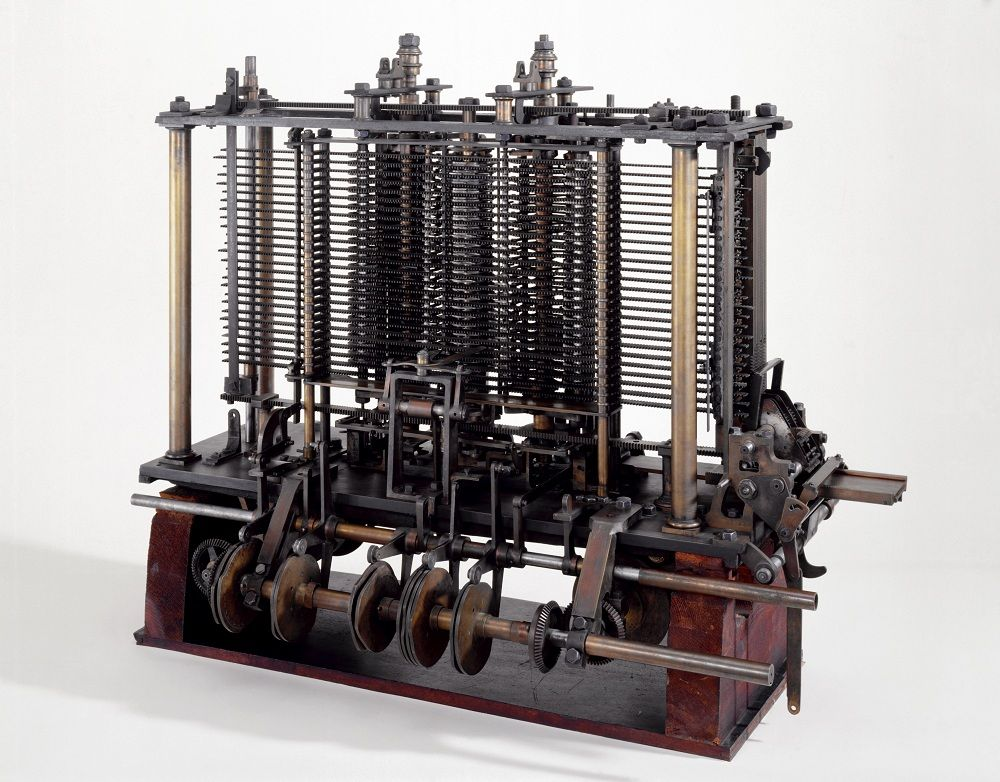
\includegraphics[width=\textwidth]{images/analytic_engine.jpg}
	\caption{Charles Babbage's Victorian-era computer, called the ``Analytical Engine.'' Ada Lovelace worked closely with Babbage and was inspired to imagine how powerful future computers would be.}
	\label{fig:analytic_engine}
\end{marginfigure}
Ada Lovelace, daughter of the poet Lord Byron, learned of the plans for the Analytical Engine. She recognized its many potential uses, and wrote a program which would have taught the machine how to carry out an advanced mathematical calculation. For this reason, Ada Lovelace is considered by many to be the first computer programmer.
\item About a century later in the 1930's, a British mathematician named Alan Turing explored the abstract idea of universal computation: a machine which could be programmed to simulate any other computing machine. Turing's idea is the theoretical basis for modern computers. When World War II began, Turing was called upon to build a version of his machine which could break the codes being used by Germany and the Axis Powers. 
\begin{marginfigure}
	\centering
	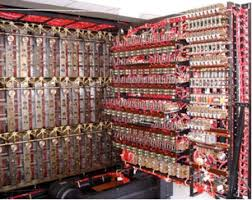
\includegraphics[width=\textwidth]{images/bombe.jpg}
	\caption{Alan Turing's code-breaking computer}
	\label{fig:bombe}
\end{marginfigure}
After the war, Turing returned to theoretical ideas, and began to wonder if computers could ever be made to ``think.'' Turing was one of the founders of the field known as artificial intelligence, which is expanding rapidly today.
\item During World War II, scientists and engineers in the United States built upon Turing's ideas, and improved the technology by building the first fully electronic general-purpose computer, called ENIAC. ENIAC was used by the United States Army to design and improve weapons, including nuclear weapons.
\begin{marginfigure}
	\centering
	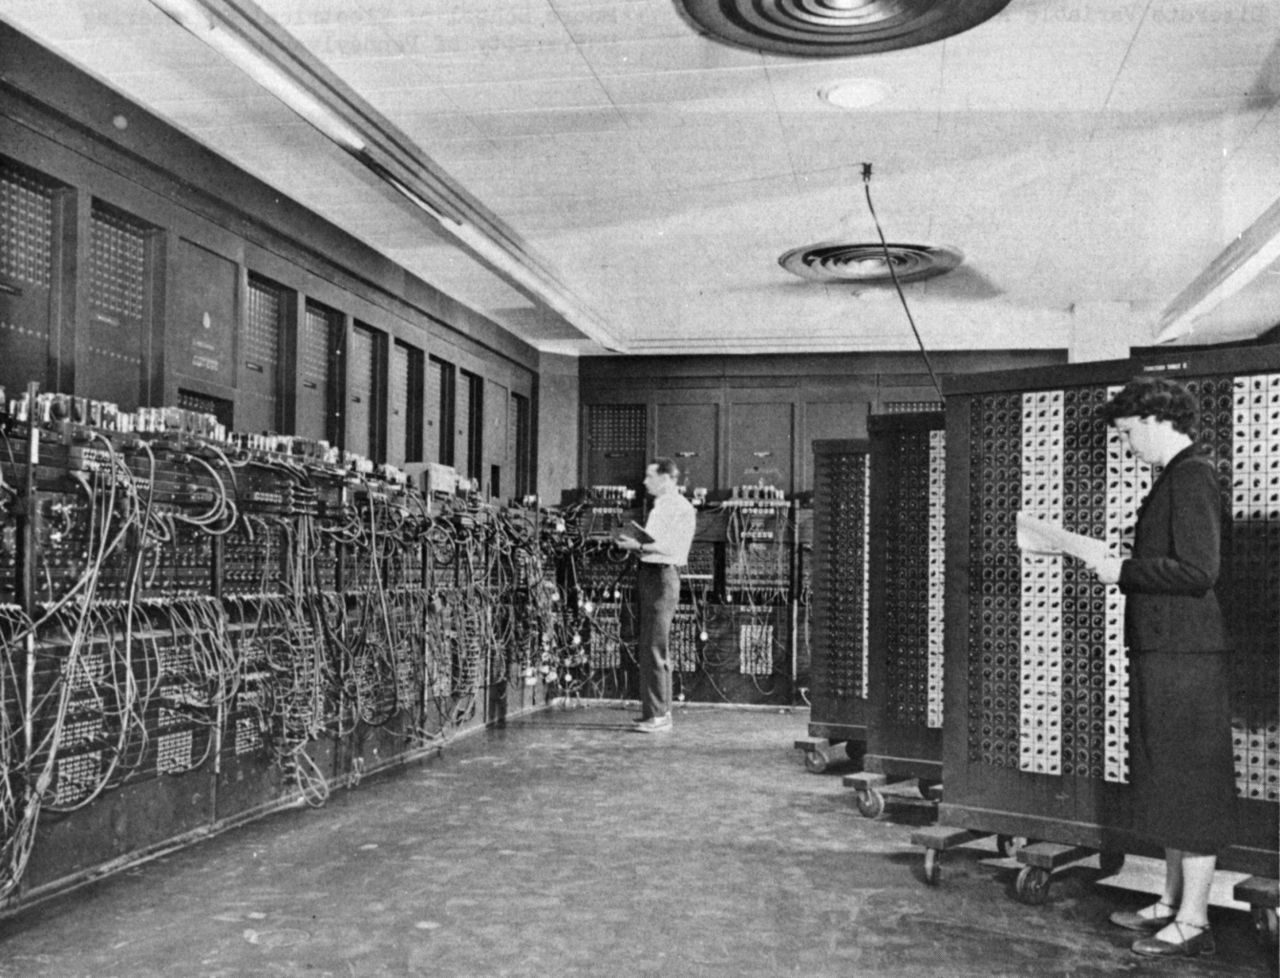
\includegraphics[width=\textwidth]{images/eniac.jpg}
	\caption{ENIAC, the first fully electronic computer, hosted at the University of Pennsylvania.}
	\label{fig:eniac}
\end{marginfigure}
\item In 1947, John Bardeen, Walter Brattain, and William Shockley succeeded in developing the first transistor, an electronic device which could replace the bulky vacuum tubes that had been used in ENIAC. This discovery won them the Nobel Prize in Physics, and allowed engineers to eventually shrink computers down to the size of a laptop or cell phone.
\item As computers became smaller and more affordable, more of them went into use, and it became important to have a way for computers to send data to each other. The United States Department of Defense designed and established the first major computer network, ARPANET, which connected several universities and laboratories across the country. The technology used in ARPANET forms the foundation for the modern Internet.
\item In 1975, Bill Gates and Paul Allen wrote software for a new kind of microcomputer which allowed them to run programs in a language called BASIC. They named their microcomputer software company Microsoft, and it became a major force in the growth of computers for personal use.
\item Shortly after, in 1977, Steve Wozniak and Steve Jobs pioneered the design of a computer engineered for usability by non-professionals. Their device, called the Apple II, was Apple's first computer intended for use in households rather than businesses.
\begin{marginfigure}
	\centering
	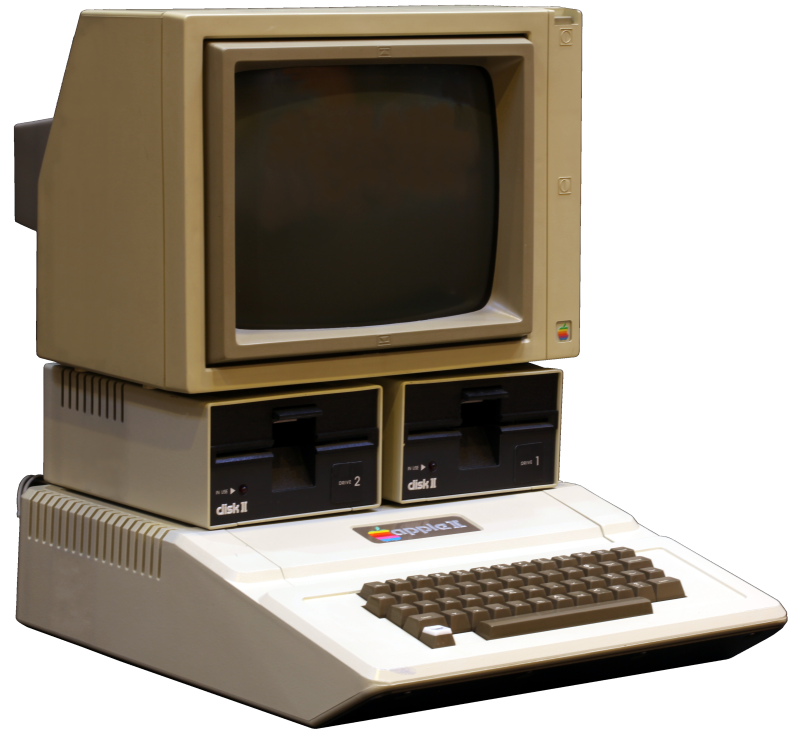
\includegraphics[width=\textwidth]{images/appleii.png}
	\caption{The Apple II, a computer built for use by non-professionals, and a precursor of modern personal computers.}
	\label{fig:appleii}
\end{marginfigure}
\item As personal computing expanded rapidly, private government and research networks like ARPANET no longer satisfied the demand for connecting computers. In 1990, Sir Tim Berners-Lee invented the World Wide Web, which allowed people to use their computers to view web pages hosted on other computers. The World Wide Web remains in use today, and has been a major driver in the growth of the computer industry.
\end{itemize}

\section{Components of a computer}

There are four primary components of a computer: its hardware, its software, its data, and its user. We'll cover each of these in more detail in later chapters, but we will give a brief overview here.

\subsection{Hardware}

Computer hardware consists of physical, electronic devices. These are the parts you actually can see and touch. Some examples (you don't need to memorize this list!) include\endnote{https://www.tutorialandexample.com/computer-hardware/}

\begin{itemize}
	\item Central processing unit (CPU)
	\item Monitor
	\item CD drive
	\item Keyboard
	\item Data storage
	\item Graphics card
	\item Sound card
	\item Speakers
	\item Motherboard
\end{itemize}

\begin{figure}
	\centering
	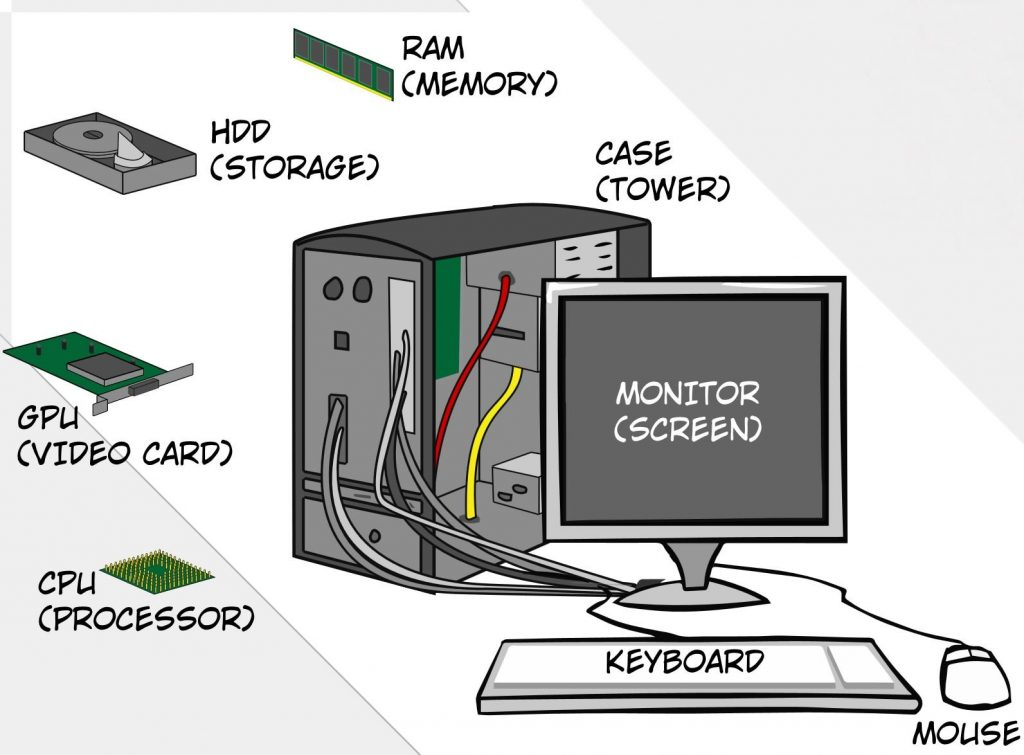
\includegraphics[width=\textwidth]{images/hardware-components.jpg}
	\caption{Examples of hardware components of a personal computer.}
	\label{fig:hardware}
\end{figure}

We will discuss these components in more detail in a later lecture. 

\subsection{Software}

Software (otherwise known as \textit{programs}, \textit{applications}, or \textit{apps}) are organized sets of instructions for controlling the computer.

There are two main classes of software:

\begin{itemize}
	\item Applications: programs allowing the human to interact directly with the computer
	\item Systems software: programs the computer uses to control itself
\end{itemize}

Some familiar applications include:

\begin{itemize}
	\item Microsoft Word: allows the user to edit documents
	\item Mozilla Firefox: connects the user to the World Wide Web
	\item iTunes: organizes and plays music files
\end{itemize}

While applications allow the user to interact with the computer, systems software keeps the computer running. The operating system (OS) is the most common example of systems software, and it schedules tasks and manages storage of data.

We will dive deeper into the details of both applications and systems software in Chapter \ref{ch:hardware_software}.

\subsection{Data}
Data is information of any kind. One key facet of computers is their ability to reliably store massive quantities of data for a long time. Another is the speed with which they can do calculations on data once they receive instructions from a human user.

While humans can understand data with a wide variety of perceptions (taste,
smell, hearing, touch, sight), computers read and write everything internally as
\textit{bits}, sequences of 0s and 1s.

Computers have software and hardware which allow them to convert their internal 0s and 1s into text, numerals, and images displayed on a monitor, as well as sounds which can be played through a speaker.

Similarly, computers have hardware and software that convert information from
the real world into bits: a microphone converts sound, a camera converts pictures, and a text editor converts character symbols.

\subsection{Users}

Of course, there would be no data and no meaningful calculations without the human user. Computers are ultimately tools for making humans more powerful.

As we will see in the next section, different types of computers have different roles for the user.

\section{Types of computers}

\subsection{Supercomputers}

Supercomputers are the most powerful computers out there. They are used for problems that take along time to calculate. They are rare because of their size and expense, and therefore primarily used by big organizations like universities, corporations, and the government.

The user of a supercomputer typically gives the computer a list of instructions, and allows the supercomputer to run on its own over the course of hours or days to complete its task.

Supercomputers generally become ``super'' by combining the capabilities of many different regular computers together. Programming a supercomputer effectively requires an advanced technique called parallel programming, which instructs a group of computers on how to share the work for a task and complete it cooperatively.\endnote{https://insidehpc.com/2018/11/new-top500-list-lead-doe-supercomputers/}

\begin{marginfigure}
	\centering
	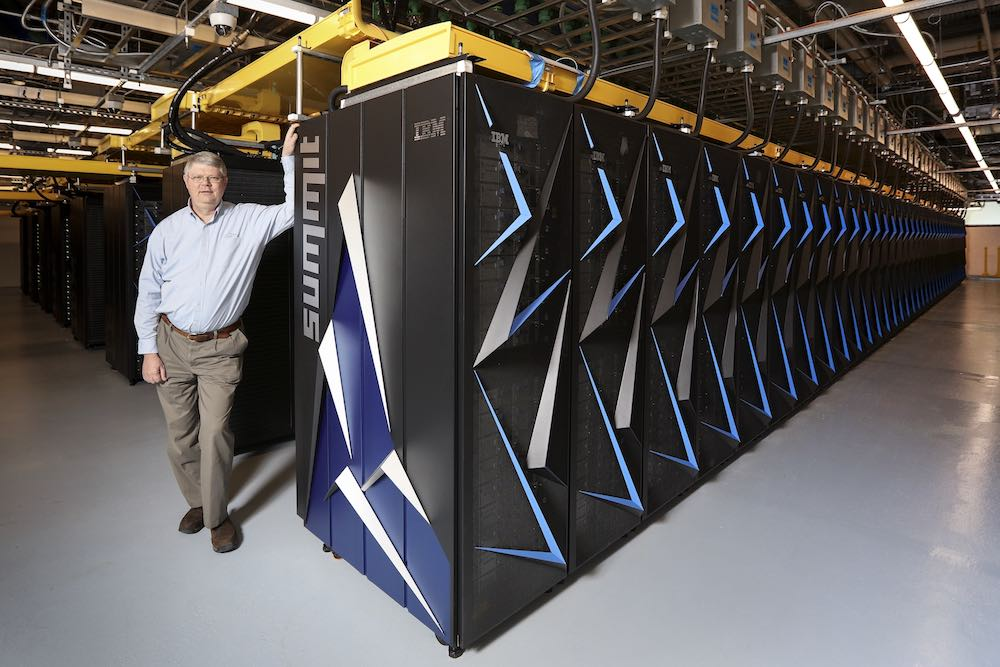
\includegraphics[width=\textwidth]{images/supercomputer.jpg}
	\caption{Summit, a world-class supercomputing cluster at Oak Ridge National Laboratory in Tennessee.}
	\label{fig:supercomputer}
\end{marginfigure}

\subsection{Mainframe computers}
Although not as powerful as supercomputers, mainframe computers can handle more data and run much faster than a typical personal computer. Often, they are given instructions only periodically by computer programmers, and then run on their own for months at a time to store and process incoming data. For example, census number-crunching, consumer statistics, and transactions processing all use mainframe computers.

\subsection{Personal computers}
These are the familiar computers we use to interact with applications every day. Full-size desktop computers and laptop computers are examples.

\subsection{Embedded computers}
In the modern ``digital'' age, nearly all devices we use have computers embedded within them. From cars to washing machines to watches to heating systems, most everyday appliances have a computer within them that allows them to function.

\subsection{Mobile computers}
In the past two decades, mobile computing devices such as smartphones have exploded in popularity, and become nearly as capable as standalone personal computers for many tasks.

\exercisesection

\pgfoonew \maze=new maze()

\begin{marginfigure}[4cm]
  \centering
    \begin{tikzpicture}[scale=.37,flag/.style={scale=.37},turt/.style={scale=.37}]
        \maze.drawMaze();
        \maze.drawTurt();
    \end{tikzpicture}
    \caption{An example maze. The roboturt starts at the box in the bottom left facing toward the top of the page. We need to get it to the box with the finish flags at the top right.}
    \label{fig:graph-paper}
\end{marginfigure}

\begin{exercise}

For this exercise you are going to program a robotic turtle (``roboturt'') to complete a maze. The roboturt accepts two commands:  ``Turn Left [number]'' (TL[n]) and ``Move Forwards [number]'' (MF[n]). The command TL tells the roboturt to change its direction without moving out of its box (and note that 3 lefts can make a right). MF tells the roboturt to step into the box in front of it. For example, the following commands would tell the roboturt to complete the example maze shown in Figure \ref{fig:graph-paper}: MF[4], TL[3], MF[6], TL[1], MF[3], TL[3], MF[3], TL[1], MF[4]. A visual representation of the roboturt following these commands is in Figure \ref{fig:turtle_sequence}.

Get a piece of graph paper, and draw your own maze on it. Make sure to draw a roboturt in the starting box in whatever direction you want it to start in, and a flag at the finish box. You may refer to the maze in Figure \ref{fig:graph-paper} as an example. 
  
First create a list of commands that tells the robot to complete your own maze. Then do the same for another student's maze. Compare your command sequences. 

What types of commands could have made this easier? Could your robot solve
arbitrary mazes? What types of commands would be helpful for making your robot
solve any maze?\safemarginnote[-2cm]{Hint: what happens if the roboturt always follows the wall to its right?}
\end{exercise}


\begin{figure}
  \centering
    \begin{tikzpicture}[scale=0.3,flag/.style={scale=.3},turt/.style={scale=.3}]
        \begin{scope}
            \maze.drawMaze();
            \maze.MF(4);
        \end{scope}
        \begin{scope}[xshift=13cm]
            \maze.drawMaze();
            \maze.TL(3);
        \end{scope}
        \begin{scope}[xshift=26cm]
            \maze.drawMaze();
            \maze.MF(6);
        \end{scope}
        \begin{scope}[yshift=-13cm]
            \maze.drawMaze();
            \maze.TL(1);
        \end{scope}
        \begin{scope}[xshift=13cm,yshift=-13cm]
            \maze.drawMaze();
            \maze.MF(3);
        \end{scope}
        \begin{scope}[xshift=26cm,yshift=-13cm]
            \maze.drawMaze();
            \maze.TL(3);
        \end{scope}
        \begin{scope}[yshift=-26cm]
            \maze.drawMaze();
            \maze.MF(3);
        \end{scope}
        \begin{scope}[xshift=13cm,yshift=-26cm]
            \maze.drawMaze();
            \maze.TL(1);
        \end{scope}
        \begin{scope}[xshift=26cm,yshift=-26cm]
            \maze.drawMaze();
            \maze.MF(4);
        \end{scope}
    \end{tikzpicture}
    %\includegraphics{maze2.png}
   % \includegraphics{maze3.png}
    \caption{A visual representation of what happens when the roboturt follows the commands (MF[4], TL[3], MF[6], TL[1], MF[3], TL[3], MF[3], TL[1], MF[4]).}
    \label{fig:turtle_sequence}
\end{figure}

\begin{exercise}
Imagine a scenario in which you have to describe how to draw a simple house (example shown in Figure~\ref{fig:house-drawing}) to a friend over the phone step-by-step. Is the instruction ``Draw a square with a triangle on top'' sufficient? What instructions would you give to obtain an accurate drawing? 
\end{exercise}

\begin{figure}
  \centering
    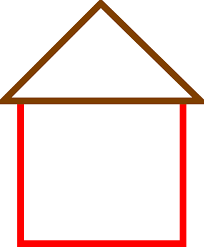
\includegraphics[width=.32\textwidth]{images/simple_house.png}
    \caption{An example of a simple house.}
    \label{fig:house-drawing}
\end{figure}

\begin{exercise}
What are some other tasks a computer can accomplish?
\end{exercise}

\begin{exercise}
  Think about building a simple video game. What are the hardware, software, and
  data needed for this game? What would be the minimal hardware, and what
  hardware would you need to add features like voice chat or online play? What
  types of computers would best run this game? Why?

  Do the same for a text editor and an ATM machine. 
\end{exercise}


\referencessection

\textit{Computer Science: An Interdisciplinary Approach}, Robert Sedgewick and Kevin Wayne.

University of Wisconsin-Madison CS 202 Lectures, Andrea Arpaci-Dusseau.\\http://pages.cs.wisc.edu/~dusseau/Classes/CS202-F11/

\theendnotes

	
% 	"Productivity" lecture should be folded into "computer review" sessions
	\chapter{Business Software}

\section{Introduction}

This lecture will go over three primary types of business productivity software most businesses use on a daily basis: 
\begin{enumerate}
	\item Word processing software: for typing and formatting text and images on a page (such as essays and reports) 
	\item Presentation software: for creating slides with information and graphics (such as for meetings and briefings)
	\item Spreadsheet software: for storing data, doing computations, and making graphs
\end{enumerate}

\section{Word Processing}

Word processing software is used for creating, editing, and formatting documents. Many tech companies have their own version of word processing software. A few more familiar examples include
\begin{itemize}
	\item Microsoft Word
	\item Apple Pages
	\item Google Docs
\end{itemize}

Beyond providing an interface to type the words of your report or essay into, word processors allow a variety of styling and formatting options to customize the document to look the way you like it. For example, all of the word processors above support
\begin{itemize}
	\item Automatic page numbering
	\item Adjustable margins
	\item Varieties of text size, text font, text color
	\item Addition of images and captions, along with image formatting
	\item Addition of tables and lists 
	\item Spelling and grammar checking
\end{itemize}

% Pop in  a picture

\section{Spreadsheets}

Spreadhseet software is used for dealing with data. A few examples of spreadsheet software include
\begin{itemize}
	\item Microsoft Excel
	\item Apple Numbers
	\item Google Sheets
\end{itemize}

Beyond providing a grid in which you can type numbers, spreadsheet software facilitate a variety of operations on the data. styling. A few key features supported by most spreadsheet applications include
\begin{itemize}
	\item Statistical analysis
	\item Sorting
	\item Creating charts and graphs
	\item Formatting (e.g. adding color, borders, etc.)
\end{itemize}

% maybe some activities here about what you would do with given data? 
% probably want to add pictures to illustrate each of the operations above 

\section{Presentations}

Presentation software is used for presenting data and graphics to an audience. Some common examples include
\begin{itemize}
	\item Microsoft Powerpoint
	\item Apple Keynote
	\item Google Slides
\end{itemize}

All of these software give the user a series of "slides" that can be clicked through during a presentation. It allows the presenter to focus the audience's attention on a single point at a time. The slides are not meant to contain all the information that the presenter wants to get across. Instead, the slides only mention the key takeaways, and the presenter should verbally fill in the details. For that reason, slides often consist of just a few bullet points and an image. Of course, there are a variety of creative ways to present - this is just the most common format!

A few particularly important features offered by almost all presentation software include
\begin{itemize}
	\item Automatic styling (color schemes, layouts, etc) 
	\item Add images and videos
	\item Slide transitions 
	\item Animations (e.g. showing one line of text on a slide at a time) 
\end{itemize}

\section{Project} 


	
    \chapter{Hardware}

\begin{figure}
	\centering
	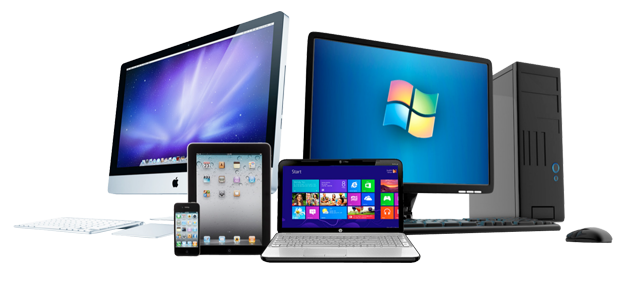
\includegraphics[width=0.85\textwidth]{images/computer_system.png}
	\caption{A variety of computer systems: desktops, a laptop, a tablet, and a
    smart phone. \afm{Source for pic.}}
	\label{fig:hardware:computers}
\end{figure}

Today's lecture will focus on \emph{computer systems} \afm{should we change the title
  to systems, this is funky to say the chapter is hardware, and then say we
  focus on systems}, groupings of devices that work together to perform a common
task (or tasks).  When most of us think about
computers, we often think of a desktop or laptop computer, equipped with a
keyboard, mouse, and monitor as seen in Figure~\ref{fig:hardware:computers}.
However, many things we interact with daily are computerized, including cell
phones, cars, traffic lights, smart watches, televisions, and manufacturing
lines. Today each of these items has sensors to perceive the real world, uses an
embedded computing device to understand the sensory input, and uses a combination
of display and mechanical devices to interact with the real world.

\begin{example}
  For intersections across busy roadways, some traffic lights are computerized
  to optimize road traffic. These lights will stay green along the busier of the
  two roads, and use cameras or pressure sensors to detect the presence of cars
  along the less busy of the two roads. When cars arrive, the lights switch,
  allowing the cars on the less busy road to cross.
\end{example}

Today we will introduce three fundamental parts of computer systems:
input and output devices, memory, and the central processing unit (CPU).
These components work together to perform the basic building blocks of
input processing, storage, control, and output. Understanding how the
three parts work together will allow us to create powerful information
processing tools. We will introduce each of these parts in turn.
In Figure~\ref{fig:hardware:overview}, we see how these parts come
together to form a computer system.

\begin{figure}
	\centering
	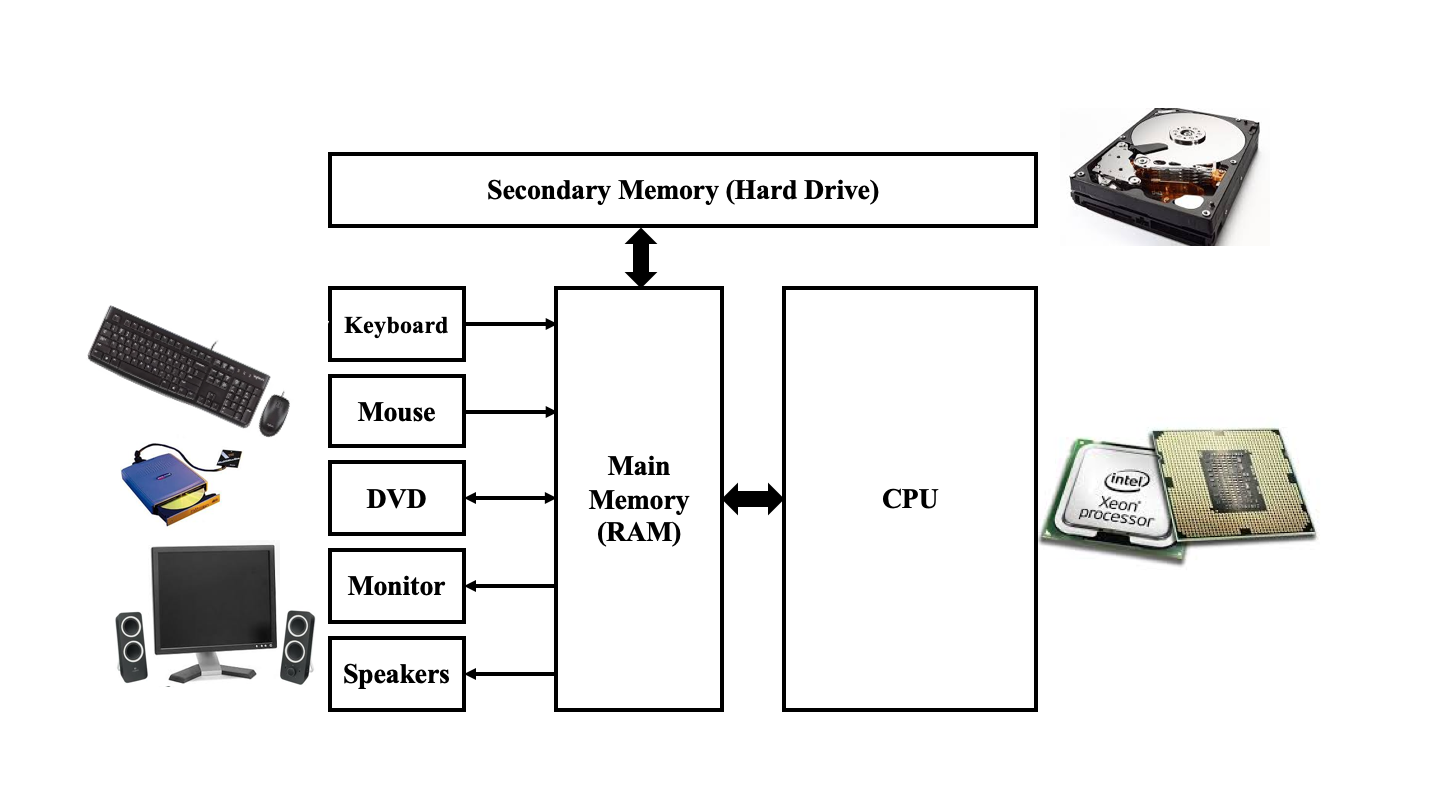
\includegraphics[width=0.85\textwidth]{images/cs_intro_hardware_overview.png}
	\caption{Interconnected parts of a computer system (keyboard, mouse,
                 monitor, DVD player / burner, speaker, hard drive, CPU).
                 \afm{source for pic}}
	\label{fig:hardware:overview}
\end{figure}

\section{Input and Output Devices}

Input and output  devices allow the computer to interact with users and the world
directly.  \emph{Input} devices are used to bring data into the computer system. Examples include keyboards, mice, and microphones. \emph{Output} devices are used to display the results or information of a computer system. The most common forms of output are words, numbers, and graphics.  Examples of output devices include speakers, printers, and monitors. With input and output devices, a
user's input will be processed, some computations will be performed, and then
the resulting output will be displayed to the user. Without these devices, a computer system would be very boring, always
performing the same computation each time it's used. Even if it did compute a
different value we would be unable to examine the value. A computer needs to be
able to accept input and output a result. The first computers would occupy a
large room in an office building and connect to a terminal (a keyboard and a
text screen) in another room for users to interact with. Thanks to the hard work
of electrical engineers,
computers can now fit in the palm of your hand while being much more powerful.
Likewise, many more types of input and output devices are now available. We
still have the keyboard and monitor, and the mouse was invented for interacting
with graphical displays. Today's phones are more computer than phone, coming
equipped with speakers, microphones, touch screens, cameras, fingerprint
scanners, radio transmitters, and much more. Computers even come embedded in
other devices like cars, traffic lights, X-ray machines, and thermostats to both
control and monitor the devices. As shown in Figure~\ref{fig:hardware:overview},
these devices connect to the rest of the computer through the computer's memory.
This kind of input and output is called memory mapped I/O (input and output).
Creators of input (or output) devices are assigned a section of the computer’s memory to write (for input devices) or read (for output devices) data. For example, a keyboard might write data about each key that is pressed to a given location. The computer will then read the data in that location to communicate with the keyboard. In the case of an output device, the process works in reverse: the computer writes the data in the assigned location, which the output device then reads. The creators of these devices agree on a known format to read and write data.

\begin{example}
  You can think of communication between devices and computer as similar to
  leaving messages for a friend in a locker. Only you and your friend have
  access to this locker, which only holds space for one message. The format you
  agree upon is which language you'll use to speak (e.g. English) and any
  special keywords or phrases. For example, you might agree upon a convention
  like the kind used in radio communication, where one person waits until they
  get an ``Over'' signal before responding with a new message.
\end {example}

The format that devices and computers communicate in are generally very simple
and structured to permit fast and easily understandable communication for
computers and devices.

\begin{example}
A monitor is a graphical display for computers. Let's consider a monitor
connected to a computer that only displays in black and white images
that are 20 x 20 pixels large. The monitor and keyboard agree upon using
the following format to communicate. The format is black and white images
that are 20 x 20 pixels large. Each pixel's value is represented at 0 for
black and 1 for white. Then an image is represented as a 400 = (20 x 20) long
sequence of pixel values. The sequence is ordered left to right, top to bottom.
Now that both the monitor and computer agree upon the communication format, the
computer can write images to the section of memory dedicated to the monitor
and the monitor will read the image and display the image on its screen.
Figure~\ref{fig:hardware:monitor_image} displays an example image, a 
20 x 20 checkerboard with its encoding.

\emph{Note: While this is a simplified example, this is similar to how modern
  graphical displays communicate with computers}.
\end{example}

\begin{figure}
	\centering
        \hspace{0.5cm}
	\begin{minipage}{0.45\textwidth}
		
\includegraphics[width=0.90\textwidth]{images/checkered_image.jpg}
	\end{minipage}
        \begin{minipage}{0.45\textwidth}
		\scriptsize
\begin{verbatim}
0 1 0 1 0 1 0 1 0 1 0 1 0 1 0 1 0 1 0 1
1 0 1 0 1 0 1 0 1 0 1 0 1 0 1 0 1 0 1 0
0 1 0 1 0 1 0 1 0 1 0 1 0 1 0 1 0 1 0 1
1 0 1 0 1 0 1 0 1 0 1 0 1 0 1 0 1 0 1 0
0 1 0 1 0 1 0 1 0 1 0 1 0 1 0 1 0 1 0 1
1 0 1 0 1 0 1 0 1 0 1 0 1 0 1 0 1 0 1 0
0 1 0 1 0 1 0 1 0 1 0 1 0 1 0 1 0 1 0 1
1 0 1 0 1 0 1 0 1 0 1 0 1 0 1 0 1 0 1 0
0 1 0 1 0 1 0 1 0 1 0 1 0 1 0 1 0 1 0 1
1 0 1 0 1 0 1 0 1 0 1 0 1 0 1 0 1 0 1 0
0 1 0 1 0 1 0 1 0 1 0 1 0 1 0 1 0 1 0 1
1 0 1 0 1 0 1 0 1 0 1 0 1 0 1 0 1 0 1 0
0 1 0 1 0 1 0 1 0 1 0 1 0 1 0 1 0 1 0 1
1 0 1 0 1 0 1 0 1 0 1 0 1 0 1 0 1 0 1 0
0 1 0 1 0 1 0 1 0 1 0 1 0 1 0 1 0 1 0 1
1 0 1 0 1 0 1 0 1 0 1 0 1 0 1 0 1 0 1 0
0 1 0 1 0 1 0 1 0 1 0 1 0 1 0 1 0 1 0 1
1 0 1 0 1 0 1 0 1 0 1 0 1 0 1 0 1 0 1 0
0 1 0 1 0 1 0 1 0 1 0 1 0 1 0 1 0 1 0 1
1 0 1 0 1 0 1 0 1 0 1 0 1 0 1 0 1 0 1 0
\end{verbatim}
        \end{minipage}
	\caption{An example checkered image and its encoding --- newlines and spaces added for readability.}
	\label{fig:hardware:monitor_image}
\end{figure}

\section{Memory}

With \emph{memory}, computers gain the ability to store and recall data. This is very
similar to physical storage of items. Figure~\ref{fig:hardware:storage} shows
three storage locations --- a storage closet, a garage, and a warehouse. Each of
the three locations make a tradeoff between convenience of location and storage
capacity. The closet can contain a few things and is the same room you need it.
The garage can fit even more things and is only a walk outside (or through) your
home, and the warehouse can fit practically anything you would want to store but
you have to drive to the warehouse to pick-up or store your items. Similarly, a
computer's memory makes the same trade-offs.

There are two major types of memory, \emph{Main Memory} (RAM) and \emph{Secondary Memory},
like hard disks, solid-state drives, tape drives, and more. Main memory is \emph{volatile},
meaning that the contents of the memory is not preserved when a computer is
turned off and back on. On the other hand Secondary Memory is meant to be
\emph{persistent} or \emph{nonvolatile}, and does not go away when the computer is turned off. Main Memory
can be thought of as the ``scratch paper'' the computer uses for computations.
Computers will also use Main Memory as a conduit for communicating between the
CPU and all other parts of the computer. Main memory is closer to a garage
(where you can lose items when you turn off the lights) --- there is enough room
to fit most items you use regularly and is close enough to not worry about the
time it takes to get to the garage.

In most modern computers,
programs are treated as data. The individual instructions that combine
to form a program are stored in memory just as data is. It is the job of the
computer to properly understand if a segment of memory is data or a program.
The computer is able to fetch data from Secondary Memory to Main Memory or
persist data in Main Memory to Secondary Memory when needed. However,
this process of transferring data between Secondary and Main Memory can
cost a lot of time relative to keeping data in Main Memory only.

\begin{figure}
	\centering
	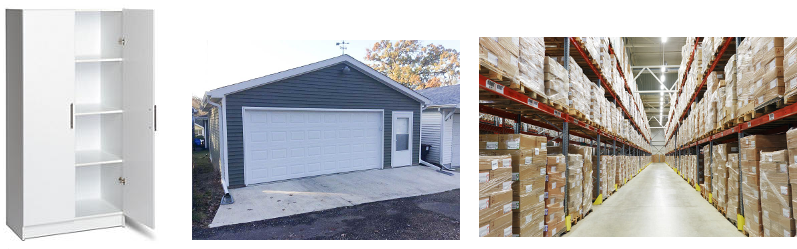
\includegraphics[width=0.85\textwidth]{images/storage.png}
	\caption{Storage closet, garage, and warehouse trading off between
                 capacity and locality. \afm{picture references}}
	\label{fig:hardware:storage}
\end{figure}

\section {Central Processing Unit}

The final part of a computer we will introduce today is the \emph{central processing
unit} (CPU), also known as the \emph{processor} or \emph{main processor}. The CPU is the physical
circuitry of a computer that performs instructions.

The CPU has several key components: the control logic, arithmetic and logic unit (ALU), registers,
program counter, and clock. These components work together to 
fetch, decode, and execute all instructions --- the building blocks of all programs.
Instructions vary between different brands of CPUs, but, in general, they will
include arithmetic, control, read (from memory), and write (to memory) functionalities.

Example~\ref{ex:hardware:instr} shows several instructions
that together would perform \ic{x = x + y}, given \ic{x} is stored in memory
location 16 and \ic{y} at memory location 20. These instructions are quite low
level, and harder for humans to read than the programs we will write in this course.
However, the programs we write will be translated into these instructions to be
easily understood and executed by the CPU.

\begin{example}
\label{ex:hardware:instr}
\begin{verbatim}
load R1 16    -- Load value at memory location 16 into register 1
load R2 20    -- load value at memory location 20 into register 2
add  R1 R2 R1 -- add the value in register 1 to the value in register 2
                 and store in register 1
store R1 16   -- store the value in register 1 to memory location 16
\end{verbatim}
\end{example}

A key component of a CPU is its clock. The clock allows the CPU to progress in time,
triggering the time to progress from time \ic{t} to time \ic{t + 1}. A single time
segment is referred to as a clock cycle. You might have heard about a computer's CPU
speed. For example, your computer may run at 2.4 GHz = 2.4 billion clock cycles per second. This
is determined by how fast the clock transitions from one time step to the next. This
clock drives the progress of the CPU. The time an instruction takes is measured
in instruction cycles. The rate of the CPU's clock is determined by the slowest
operation of the CPU.

In addition to clocks, the CPU contains a group of memory locations called registers.
A single register is capable of holding a single ``word'' of information. A ``word'' is the smallest
unit of data in a computer. The key benefit of registers is the ability for the
CPU to immediately read and write the contents of the register. The value of a register
can be updated each time the computer's clock ``ticks,'' or increments its value by one. 
Most modern CPU's will have between 16 and 64 registers that programs may use.
For comparison, accessing Main memory can take 10s or even 100s of instruction
cycles to access while registers are immediately available to the CPU.

The control unit and program counter will fetch, decode, and output the
controls for the execution of each instruction. The program counter holds the
location of the next instruction to be executed. The next instruction is then
fetched to the CPU. The CPU's control unit then decodes the fetched instruction
and outputs control signals (commands) to main memory and the ALU. The CPU may
read data from memory (e.g. store) and then the ALU will then execute the action
specified by the control unit. Example actions include add, subtract, multiply, compare to 0, etc.
The CPU may then possibly write the output to memory.

In most computers, the CPU and its constituent parts are responsible for all
computing needs of the computer. In some select systems, there will be additional
hardware to perform specialized operations (e.g. graphics processing units for
processing / producing images). It is the CPU's responsibility to control the
computer and coordinate with devices to execute programs. As such, the CPU
has seen a quick evolution to increase its processing power. Electrical
engineers originally focused on making the CPU smaller and smaller and thus
quicker. The evolution follows Moore's Law : every two years the size of a CPU shrinks
in half. Additionally, CPU's were designed with a pipelining architecture: this means
that multiple instructions are executed in quick succession. This is done
by noting that each stage of the five stages --- fetch, load,  decode, execute,
and store --- can be performed independently. Thus, while one instruction is
being executed, the next instruction can be decoded. Figure~\ref{fig:hardware:pipeline}
shows how pipelining is performed by executing the different parts of the pipeline
in parallel for five consecutive instructions.

Due to the decline of Moore's Law in recent years, many CPU designers focus on
increasing processing power by improving parallelism (i.e. being able to execute
multiple instructions at a time). This allows instructions that do not depend
on each other to be executed at the same time. These CPUs are referred to as multi-core,
as they have multiple cores that each have their own set of registers, control unit,
ALU, and program counter but share main memory and a single clock. In this class we will not
teach how to effectively harness parallel programming, but note that this is
an important progress in how hardware has evolved.

\begin{figure}
	\centering
	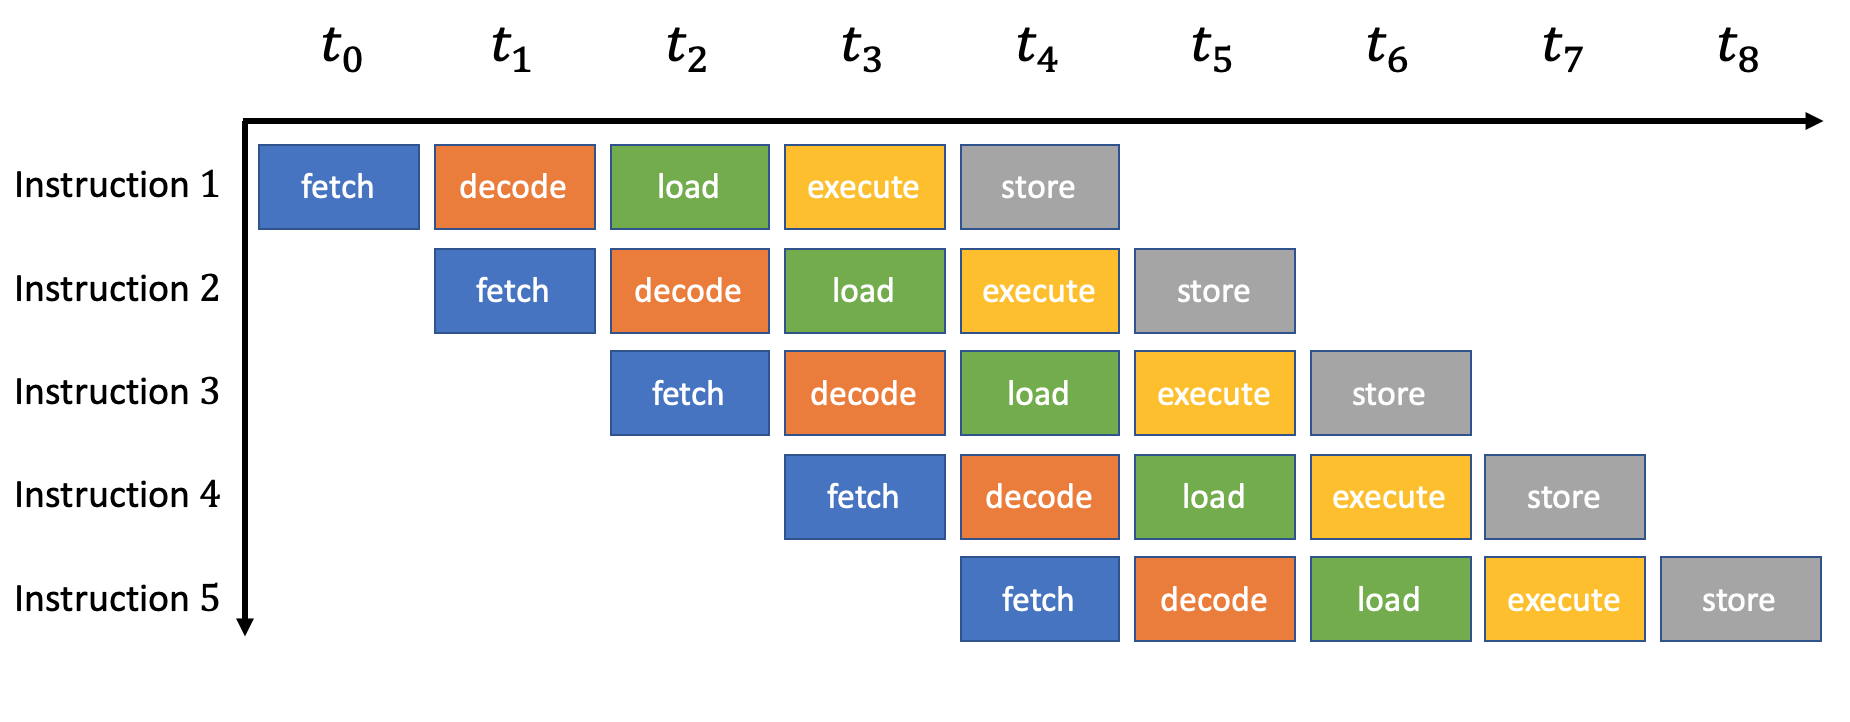
\includegraphics[width=0.85\textwidth]{images/pipeline.png}
	\caption{Instruction Pipelining. \afm{citation}}
	\label{fig:hardware:pipeline}
\end{figure}


\section {Conclusion}
In this chapter, we covered the three fundamental parts of a computer system:
input and output devices, Main and Secondary Memory, and the CPU. We discussed
their roles, relationships, and basic capabilities. I hope that this will help
you better understand how hardware works at a high level to better improve how
to write programs that will eventually run on these computer systems. In the
next chapter we will begin discussing the concept of Software and how its
similarities and differences to hardware and where the boundary between the two
lies.

\exercisesection

\begin{exercise}
What three parts comprise a computer system?
\end{exercise}

\begin{exercise}
What are examples of common input and output devices?
\end{exercise}

\begin{exercise}
Name an uncommon example of a computer system and explain how it may work.
\end{exercise}

\begin{exercise}
How does memory mapped input and output work?
\end{exercise}

\begin{exercise}
Name four kinds of memory devices.
\end{exercise}

\begin{exercise}
Explain the difference between Main and Secondary Memory.
\end{exercise}

\begin{exercise}
What parts comprise the central processing unit (CPU)?
\end{exercise}

\begin{exercise}
Describe three possible methods to increase the computation power of a CPU.
\end{exercise}

	
    \chapter{Software}\label{ch:hardware_software}

\begin{goals}
\item Understand why computers need both hardware and software.
\item Learn how software is built up of many layers, from machine code up to applications.
\item Understand generally how different layers of hardware and software interact with each other.
\end{goals}

For a long time, people have desired or imagined machines that can compute. Why did it take so long for computers to be invented? Part of the reason is that digital electronics are a relatively recent innovation, building on an understanding of the physics of materials which only came to fruition in the 20\textsuperscript{th} century. However, perhaps a more overarching difficulty is that ``machines that can compute'' is a rather poorly defined idea. What does it mean to compute?

For instance, imagine a 19\textsuperscript{th} century engineer trying to build a computer out of mechanical parts. First he might desire a machine which can add very large numbers. He spends weeks at the drawing board, sketching out a massive contraption with marbles representing digits, funnels to combine digits, gears and pulleys driving dumbwaiters which can physically ``carry the 1,'' and so on. When used just so, it can add up to five-digit numbers. Our engineer thinks he might be able to get up to eight-digit numbers with some more funding, so he presents his prototype to Queen Victoria.

``Fabulous!'' she exclaims. ``Now show me multiplication!'' Our engineer is taken aback. ``Well, your majesty, you see -- this is an adding machine. It does not multiply.'' Victoria's smile quickly fades. ``Oh. Very well then. It does not multiply. What else can it do? Could you extract the third root of 47? Sort a list of a million 32-bit integers? Compute the shortest path between two vertices on a graph?'' For Victoria was a very forward-thinking queen.

``No, your majesty -- I'm afraid this is only an \emph{adding machine}. Perhaps with a royal grant I could build many large contraptions, one for each of the tasks you have set before me.'' Victoria now wears a distinct frown. ``Goodness me,'' she exclaims. ``That just won't do. Imagine all the different computational tasks one might like to carry out. My coffers are not without bound. I cannot fund them all. It is true that separate mechanical tasks require separate machines -- I am perfectly willing to give one grant for the design of a tractor, and another for a pencil sharpener. But a \emph{computer} should \emph{compute}, in some universal sense. I shall not waste my time with adding machines and multiplying machines and root-finding machines and a thousand other such knick-knacks.''

Queen Victoria's suggestion is prescient: one might imagine a machine which can be configured to perform any sort of computational task. In the 1930's, Alan Turing (a figure whom we met briefly in Chapter \ref{chap:intro}) laid the foundations for computer science by giving a mathematical description of just such a machine. With nothing but memory and a simple CPU, it can be set up to read instructions from its memory, and then proceed to follow these instructions, manipulating subsequent data in whatever way was specified. This machine is known today as the \emph{universal Turing machine}.

The actual computers we have today are more complicated than the universal Turing machine, but they exhibit the same fundamental split. The \emph{hardware} -- that is, the bare metal that makes up the physical computer and its associated devices -- is capable of performing any kind of computation. It is left to programmers to create \emph{software}, sets of instructions which tell the hardware exactly what computations to carry out. By using different software, the same hardware can perform all of Queen Victoria's tasks, and a great deal more.

In this chapter, we will give a general overview of the many layers that allow software to run, starting with their programs at the top and ending with the hardware at the bottom. This is the first example you will see of a layered architecture\marginnote{Here, ``architecture'' refers to the design of a computer system.}; examples of the layers we will discuss are shown in Figure \ref{fig:hw_sw:layers}. We will see a similar structure in the following chapters when we discuss networks. In each case, remember that although all layers are important to understand, as a programmer you will interact mostly with the top layers.

\begin{figure}
    \centering
    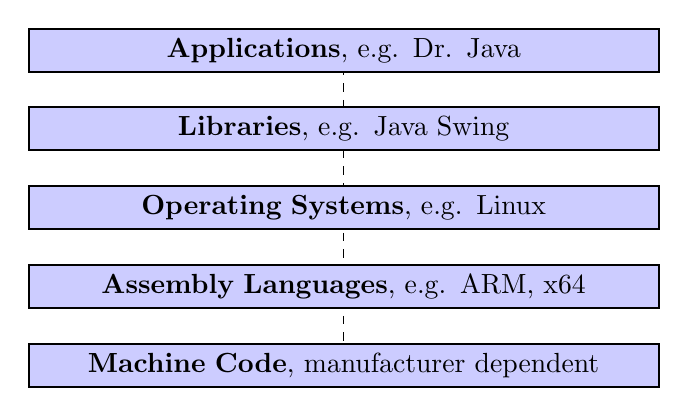
\begin{tikzpicture}[layer/.style={fill=blue!20,minimum width=8cm,align=center,text width=7.5cm,draw=black,solid,line width=.25mm}]
        \draw[dashed,-latex] (0, 4) node[layer] {\textbf{Applications}, e.g. Dr. Java} --
        (0, 3) node[layer] {\textbf{Libraries}, e.g. Java Swing} --
        (0, 2) node[layer] {\textbf{Operating Systems}, e.g. Linux} --
        (0,1) node[layer] {\textbf{Assembly Languages}, e.g. ARM, x64} --
        (0,0) node[layer] {\textbf{Machine Code}, manufacturer dependent};
    \end{tikzpicture}
    \caption{An application such as Dr. Java relies on many layers below, ending with hardware at the bottom.}
    \label{fig:hw_sw:layers}
\end{figure}

\section{Applications}

When you use a computer, you run various applications which perform tasks for you. A computer user might use a web browser to view pages on the Web, a word processor to make flyers, an email client to send messages, a Minesweeper game to kill some time -- all before lunch. Each of these is a separate application, designed by one or more programmers. Dr. Java is also an application.

In the early days of computing, applications were built from the ground up. In fact, one of the earliest ``applications,'' designed in part by Alan Turing himself, was used to break German codes during World War II. This application ran on a computer that was the first of its kind, and so every single detail had to be specified, from such high-level tasks as the mathematical cryptanalysis used to break the codes, all the way down to low-level tasks such as delivering output to the user.

Today, there are systems in place that enable programmers to create new and exciting applications without having to repeat all of the mundane parts that all applications share. Many of these more mundane parts are provided by libraries.

\section{Libraries}

Dr. Java was written using Java itself. The programmers wanted to make an application that could edit and run Java programs. But in order to do this, they need to have a way to display an editable text box containing your code, a way to display your files and let you select one to open, and so on. None of these features were programmed by hand for Dr. Java. Instead, the Dr. Java programmers made use of \emph{libraries}, code which performs common functions and which is made available for any programmer to use. Dr. Java in particular uses a library called Swing, which provides tools for programmers to develop graphical user interfaces (GUIs) using Java.

Libraries are a key component of just about any program. Different libraries may be useful in different contexts. For example, programmers designing websites need libraries which can understand how to determine the current time for users across different timezones, or libraries that understand how to securely store passwords in a database. Programmers designing artificial intelligence systems need libraries which can run digital brains known as artificial neural networks. These libraries are all provided so that nobody has to reinvent the wheel, and programmers can spend their time developing new and exciting applications.

\section{Operating Systems}

Computers today run many different applications, often all at the same time. You might run Dr. Java while using a web browser to read the Java docs and a file explorer to find where you saved your program. Each of these applications wants to use the CPU to run, access the hard drive to view files, display graphics on the screen, and listen for keystrokes from the keyboard. How does the computer manage to balance the needs of all these applications?

This is the job of an \emph{operating system}. The operating system is a special piece of software on a computer which serves as the bedrock for all other software. It is responsible for allocating resources such as CPU time and hard drive access among various applications, managing low-level functionality such as drawing graphics on the screen, and so on. In this class we are using a version of the Linux operating system, which you will learn more about in the next chapter. Other popular operating systems include Microsoft's Windows and Apple's OS X.

\section{BIOS}

Today, it is very likely that the first software loaded onto any computing device is firmware. Firmware is software that helps facilitate other software interacting with the computer device. One notable piece of firmware is called the BIOS (Basic Input/Output System). You would be hard-pressed to find any personal computer or smartphone that doesn't have a BIOS already pre-installed by the device's manufacturer. A BIOS helps facilitate initial loading of programs onto a computer. A BIOS will tell the computer to look for a connected device trying to communicate with the computer (e.g. CD or USB drives). 

\begin{figure}
    \centering
    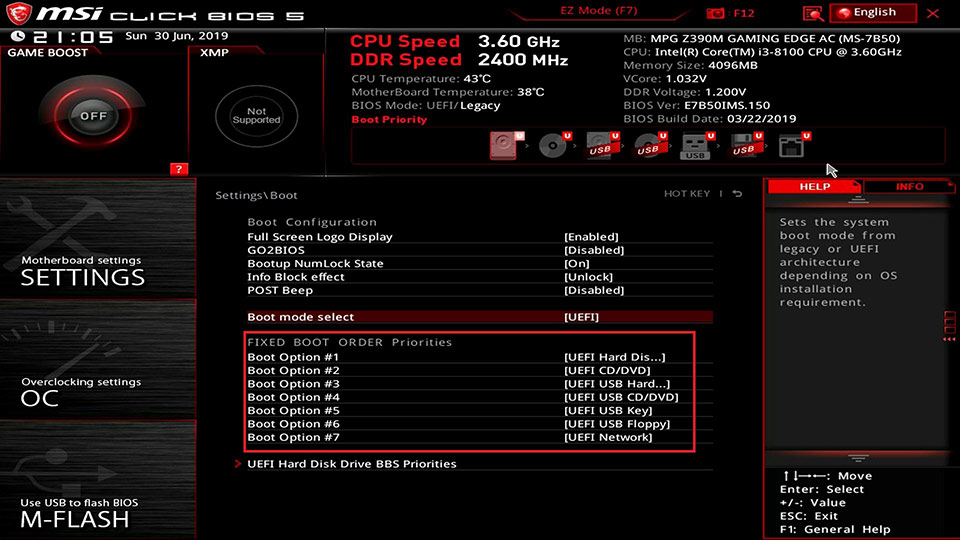
\includegraphics[width=\textwidth]{images/bios.jpg}
    \caption{The BIOS, shown here, allows a user to interact with and control basic features of a computer.}
    \label{fig:hw_sw:bios}
\end{figure}

Figure \ref{fig:hw_sw:bios} shows a relatively modern and user-friendly BIOS interface, with the settings for boot order highlighted. In this instance, the BIOS is set to first boot from an operating system on the hard disk, if one is available. This is the typical scenario for a computer which has already been set up. If there is no operating system on the hard disk, the BIOS is configured to try to boot from a CD or a USB drive instead. These devices might be used to initially install the operating system.

\section{Machine Code}

As we learned in the previous chapter, hardware is the collection of physical devices that make up a computer. The hardware performs the actual computations by manipulating electrical currents. Today most computers are digital, meaning that the computer works by representing data with electrical currents at a high or low voltage. We think of these high-voltages as ones and low-voltages as zeroes. The only thing the hardware understands are these voltages. Different sequences of voltages represent different instructions to the machine. This translation between voltages, or the corresponding binary numbers, and instructions is called the computer's machine code. Not all computers recognize the same machine code. The same sequence of ones and zeroes may not represent the same information on two computers, and it is often manufacturer dependent.

\section{Assembly Language}

In order to make it easier to write software for their computers, manufacturers will provide another language called assembly language. Typically the assembly language is one of a few popular choices. Most processors today recognize the ARM or the Intel x64 assembly languages. Assembly language is more human-readable than machine code. For example, ARM provides the instruction \ic{ADD} for adding values, and \ic{ADD r3, r1, r2} is a line of assembly language meaning add the values of \ic{r1} and \ic{r2} and store the result in \ic{r3}. The machine code equivalent would be some string of ones and zeroes.

Even though assembly language is a bit easier to understand than machine code, human programmers couldn't get very far if they had to write in assembly language. This is why we have programming languages and compilers. Languages like Java, C++ and others are designed to be relatively straightforward for humans to understand. This way, programmers can specify what they want a program to do in a way that makes sense to them. When the programmer presses compile, a compiler translates the programmer's code into assembly language. The compiler is sort of like a robot programmer: it knows how to read a program in a language like Java, and it understands it as a very precise description of a program that it should write in assembly language. 

% \section{Java Virtual Machine}

% For a long time, the model we have discussed so far worked well. A program written in an old language, such as C, would be compiled. The compiler would translate the programmer's C code into assembly language, and then the assembly code could be run on the programmer's computer. If the programmer wanted the program to run on a computer with a different assembly language, they could compile their program with a compiler written for that assembly language, and distribute that version of the compiled code accordingly.

% This changed when the Internet was created. Suddenly, instead of sending floppy disks or CD-ROMs in the mail to specific intended users, it became possible -- in principle -- to distribute a program broadly by making it available on the Internet. However, since the end user could be using a computer which understands one of many possible assembly languages, the programmer would have to make many different versions of the program available. Even if the programmer could compile her program for every possible assembly language, the user would have to know which version to download, which could be difficult.

% Java was created largely to address this issue. When you compile a Java program, you get a \ic{.class} file, which cannot be executed directly by your computer. Instead, you run \ic{java MyClass.class}, which loads a program called the Java Virtual Machine, or JVM. The JVM essentially simulates a computer with a fixed assembly language. When you downloaded the Java Development Kit, part of it was a tool called the Java Runtime Environment which operates the JVM. This way, there is only one way to compile a Java program: you run \ic{javac} and produce a \ic{.class} file. You could put this \ic{.class} file on the Internet, and another Java user could download it and run it on their JVM. The only computer-specific software is the JVM itself, which is available for any kind of computer.

\exercisesection

\begin{exercise}
    Describe the differences between hardware and software. Why is it important to have both?
\end{exercise}

\begin{exercise}
    For each of the following tasks, say which aspect of a computer or a program carries them out.
    \begin{itemize}
        \item Translate programmer's code into assembly language.
        \item Allocate CPU time to different applications.
        \item Provide reusable code to programmers.
        \item Carry out instructions specified by sequences of voltages.
        \item Look for bootable media to assist with installing an operating system.
    \end{itemize}
\end{exercise}

% \begin{exercise}
%     If assembly languages didn't exist, and hardware only understood their machine code, there would have to be more different versions of which kind of software?
% \end{exercise}

% \begin{exercise}
%     When you compile a Java program, what kind of file do you get? What software is used to run this file?
% \end{exercise}
    
    \chapter{Hello World}

It is now time for us to start practicing coding skills.
In this course, we will be focusing on learning how to program
in Java, which is just one of many programming languages.
While each programming languages has its own quirks and features
specific to it, many of the concepts you will learn in this
class will exist not only in Java but also in other languages.

We will now write our first program in Java called ``Hello World.''
We will use DrJava to help us write, compile, and run this program.

\section{Starting DrJava}
TODO: how to start DrJava on laptop that students are given
TODO: add screenshot of DrJava when just opened and label parts

On the left-hand side of the window, there is a list of currently-open files. When you first start up DrJava, the only thing there should say ``(Untitled)''.
The main part of the window is where you will write code. There should be numbers along the left-hand side to make it easy for you to see which line you are writing code on. The bottom part of the window is where we can interact with the program, for example by seeing the output of compiling the program or by seeing the output of running the program.

\section{Writing Hello World}

In the main part of the window, type the following code:
\begin{code}
class HelloWorld {
    
    public static void main(String[] args) {
        System.out.println("Hello World!");
    }
    
}
\end{code}

We will learn more about what the different parts of this program do later on, but here is a brief explanation for now:
\begin{enumerate}
\item In line 1, \ic{class HelloWorld} makes a new \emph{class} called \ic{HelloWorld}. In Java, all code must be enclosed in a class. The class contains all the code between the open curly brace \ic{\{} on line 1 and the close curly brace \ic{\}} on line 7.
\item Line 3 makes a new method called \ic{main}. We will learn later what
\ic{public static void} and \ic{String[] args} mean. For now, all you
need to know is that every Java program needs a \ic{main} method and starts
by executing the code within the \ic{main} method. Our \ic{main} method
contains all the code between the open curly brace \ic{\{} on line 3 and the
close curly brace \ic{\}} on line 5.
\item Line 4 is a print statement. \ic{System.out.println} will print out
whatever is specified between the open parenthesis \ic{(} and close
parenthesis\ic{)} that follows immediately after.
\ic{System.out.println} will begin a new line after printing out whatever is specified in the parentheses.
In this case, we
put the \emph{string literal} \ic{"Hello World!"} in between these parentheses.
String literals refer to text between quotation marks.
\end{enumerate}


\section{Saving and Compiling in DrJava}

In the upper part of the window, you should see a toolbar with many buttons.
You can now click the ``Save'' button. 

First, navigate to your Desktop folder. Once there, create a new folder called CS103 (see Figure \ref{fig:helloworld:sec:saving}). We will store all of our files for the semester in this folder. 

\begin{figure}[ht]
	\centering
	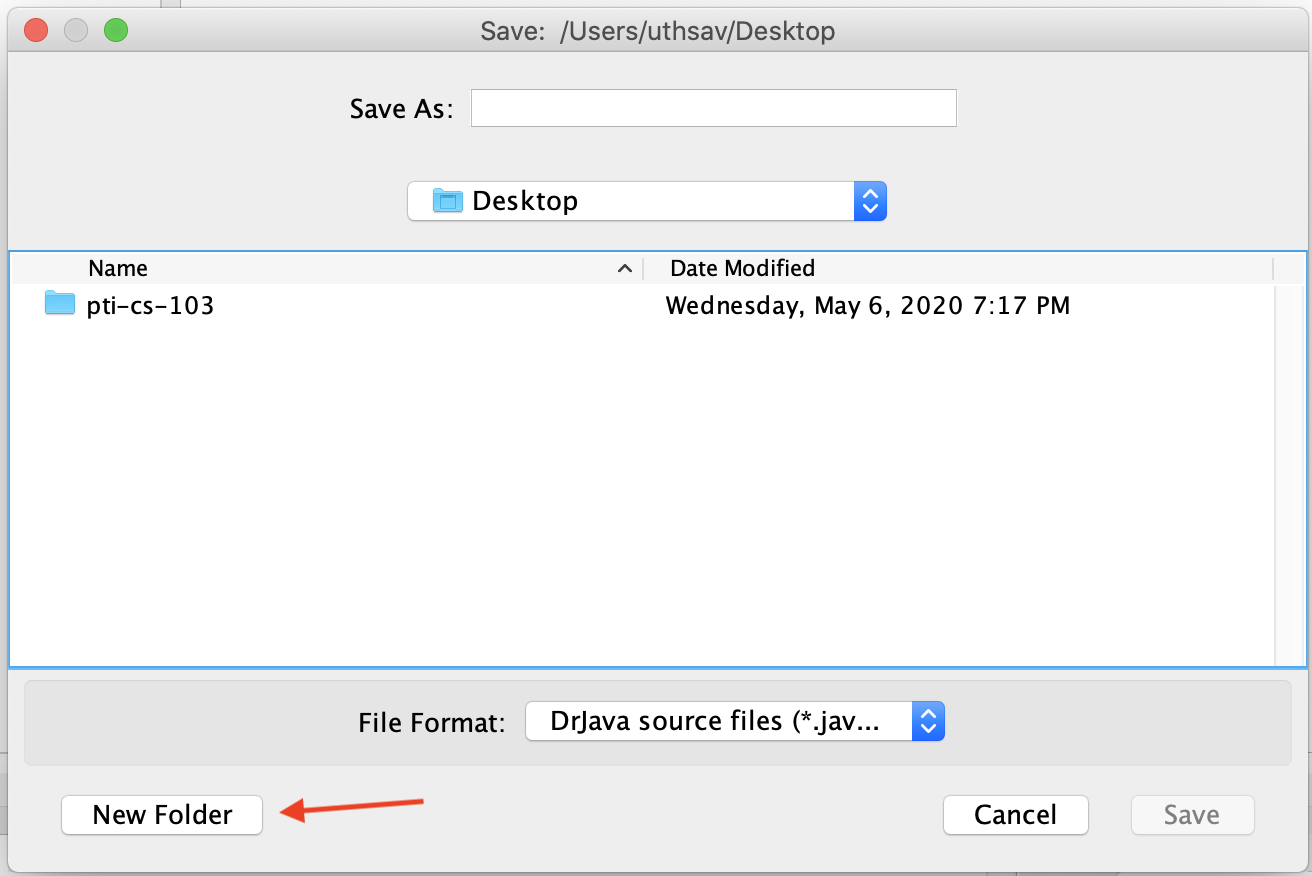
\includegraphics[width=0.85\textwidth]{images/hello_world_saving}
	\caption{Creating a CS103 folder inside your Desktop.}
	\label{fig:helloworld:sec:saving}
\end{figure}

Next, make another folder, called ``Chapter\_2", inside the CS103 folder for this class's assignment see Figure \ref{fig:helloworld:sec:saving2}).

\begin{figure}[ht]
	\centering
	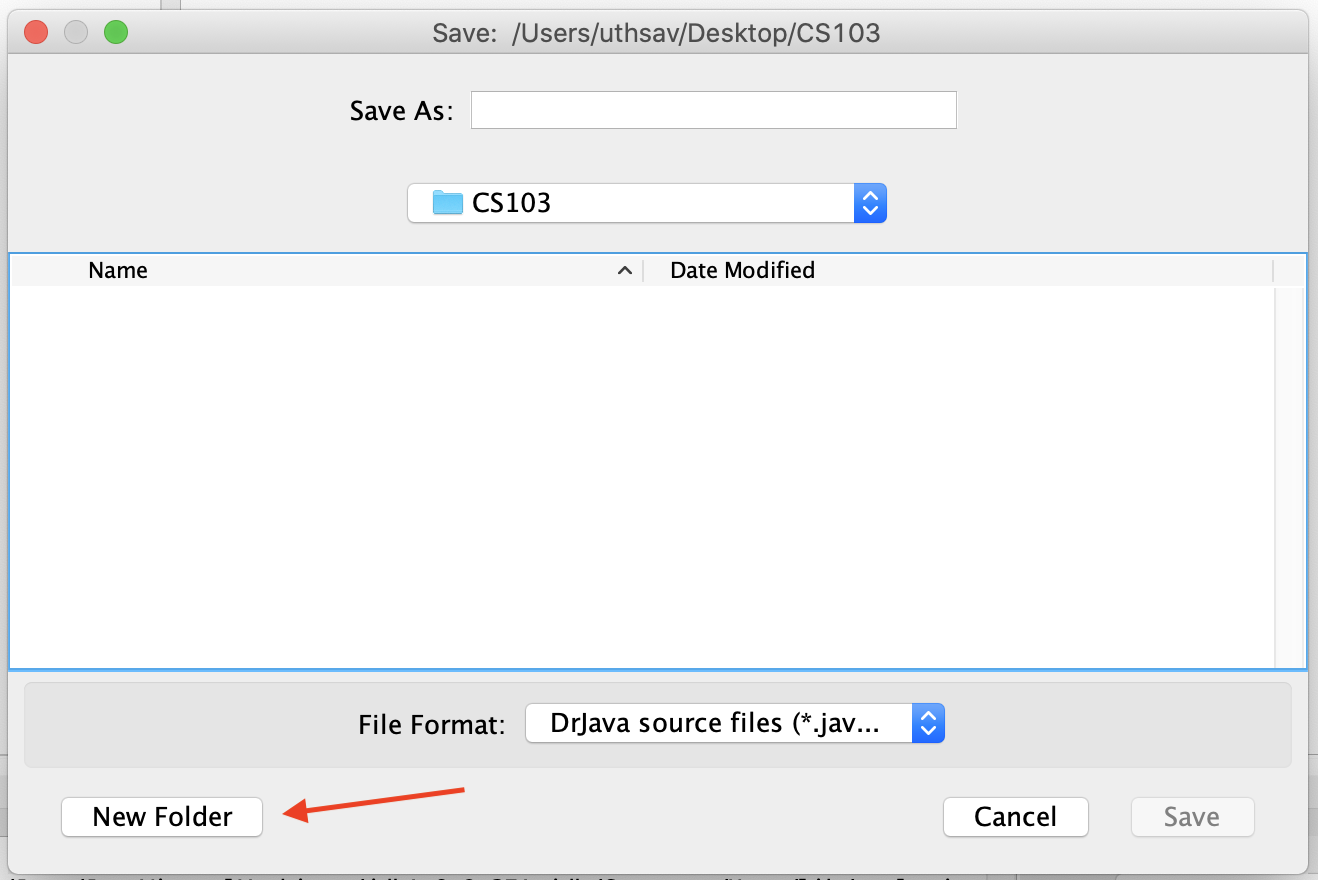
\includegraphics[width=0.85\textwidth]{images/hello_world_saving2}
	\caption{Creating another folder inside the CS103 folder.}
	\label{fig:helloworld:sec:saving2}
\end{figure}

Finally, save your file inside this folder. Because the class name is \ic{HelloWorld}, the name of your file will be
\ic{HelloWorld.java}. The \ic{.java} file extension is used for
\emph{source code}, which in this case is human-readable code written in Java.

Clicking the ``Compile'' button will first save your file (if it hasn't already been saved) and then \emph{compile} it. Compiling converts your human-readable
source code into code that is easier for the computer to read.
In the case of Java, this will generate a \ic{.class} file. The
\ic{HelloWorld.class} file contains the compiled code.
After clicking ``Compile,'' the bottom part of the window should say
\ic{Compilation completed.} If there are problems with your program, it may not be able to be compiled. In such a case, this bottom part of the window will instead indicate that there was an issue with compilation.
We can try seeing how this might look now.

Try deleting the final curly brace \ic{\}} from the program and hit ``Compile.''The bottom window should now indicate that something has gone wrong.
The message \ic{Error: reached end of file while parsing} arises because
the end of the file was reached without finding the final curly brace.
Add the curly brace back in and hit ``Compile'' again to recompile the program.
Note that in the bottom part of the window, the ``Compiler Output'' tab is selected. This tab is where you can view any messages from compilation.

Let's see another example of a compilation error. Try deleting the semicolon \ic{;} from the program and hit ``Compile.''
The message \ic{Error: ';' expected} arises because the curly brace on line 5 was reached without the semicolon being
encountered. In Java, every statement must end in a semicolon. In this case, the print statement on line 4 must
end in a semicolon. Add the semicolon back in and recompile the program. Compilation should succeed.

\section{Running Code with DrJava}
Now that the program has been written and compiled, it is now time to run it.
We can use DrJava to run a compiled program by clicking the ``Run'' button in the toolbar. In the bottom part of the window, you should see something like the following:
\begin{code}
> run HelloWorld
Hello World!
>
\end{code}
The \ic{run HelloWorld} part indicates that the program \ic{HelloWorld} should be run, and the next line is the output of the program.
Note that in the bottom part of the window, the ``Interactions'' tab is now
selected. This tab allows you to interact with your program. Clicking
the ``Run'' button is equivalent to clicking the ``Interactions'' tab, typing
\ic{run HelloWorld}, and then hitting enter/return key on your keyboard.

If you would like, you can type \ic{run HelloWorld} after the final \ic{>} and
type the enter/return key to run your program again.

\section{Making Changes}
Now we've successfully written, compiled, and ran our first Java program.
As an exercise, let's make our ``Hello World!'' more enthusiastic.
Change the \ic{Hello World!} in line 4 to \ic{Hello World!!}.
You can compile and rerun your program to see the results. In general,
you can make changes to your program, recompile it, and run it again
to see the results of your changes.

Let's make some other changes.
Try adding \ic{ //print hello} to the end of line 4, so that your line 4 now looks like this:
\begin{code}
        System.out.println("Hello World!!"); // print hello
\end{code}
Try compiling and running the program. The behavior should remain unchanged from the previous time you ran the program.
Two forward slashes \ic{//} denote the beginning of an \emph{inline comment} and have the effect of
turning the rest of the line into a \emph{comment}. Comments are ignored by the compiler and do not have any effect on
the program's behavior. They are
useful for adding explanations or providing information to people that are reading the code. In this case,
the comment \ic{print hello} can be viewed as explaining the purpose of the code on that line.

Now try adding \ic{//} to the beginning of line 4, so that it looks as follows:
\begin{code}
//        System.out.println("Hello World!!"); //print hello
\end{code}
Try compiling and running the program now. You should find that there is now no output. The two forward slashes that you added turned the whole line into a comment. As far as the compiler is concerned, your program is the same
as if the entire line 4 did not exist.

Uncomment line 4 by deleting the forward slashes you added at the beginning of it.
Now add the following lines after line 4:
\begin{code}
System.out.println("Hello!"); // print hello again
System.out.println("Goodbye World!"); // say goodbye
\end{code}
Your code now has \emph{multiple statements}. In particular, you now have three. The first one on line 4 will print
\ic{Hello World!!}, the second one will print \ic{Hello!}, and the third will print \ic{Goodbye World!}.
Note that each of these statements is followed by a semicolon.
Deleting any one of these semicolons will result in a compilation error (give it a try!).
Your code should now look as follows:
\begin{code}
class HelloWorld {
    
    public static void main(String[] args) {
        System.out.println("Hello World!!"); //print hello
        System.out.println("Hello!"); // print hello again
        System.out.println("Goodbye World!"); // say goodbye
    }
    
}
\end{code}
Try compiling it and running it. The output should look as follows:
\begin{code}
Hello World!!
Hello!
Goodbye World!
\end{code}

Let's add some description of what we're doing by adding a \emph{block comment}.
A block comment begins with \ic{/*} and is ended whenever \ic{*/} is encountered.
It may (but does not necessarily need to) span multiple lines.
Right before the main method, add a block comment to get the following:
\begin{code}
class HelloWorld {

    /* Main method to print out the following:
         Hello World!!
         Hello!
         Goodbye World!
    */
    public static void main(String[] args) {
        System.out.println("Hello World!!"); //print hello
        System.out.println("Hello!"); // print hello again
        System.out.println("Goodbye World!"); // say goodbye
    }

}
\end{code}
If you compile and run the program now, it should have the same behavior as before, since whatever occurs
inside comments does not affect the program's behavior.

Inline comments can be nested inside block comments, so for example, the following program
will compile without issue:
\begin{code}
class HelloWorld {

    /* Main method to print out the following:
         Hello World!!
         Hello!
         Goodbye World!
    */
    public static void main(String[] args) {
        /*
        System.out.println("Hello World!!"); //print hello
        System.out.println("Hello!"); // print hello again
        System.out.println("Goodbye World!"); // say goodbye
        */
    }

}
\end{code}
Note that since we have commented out all the code in the main method,
this program is actually the same as the following program that we considered earlier:
\begin{code}
class HelloWorld {

    public static void main(String[] args) {
//        System.out.println("Hello World!!"); //print hello
    }

}
\end{code}

Let's now consider the following program that has two print statements and no comments:
\begin{code}
class HelloWorld {

    public static void main(String[] args) {
        System.out.println("Hello!");
        System.out.println("Goodbye!");
    }

}
\end{code}
Try compiling and running the program. Note the output.
What happens when we remove the linebreaks and spaces between each pair of print statements?
Try removing them to get the following:
\begin{code}
class HelloWorld {

    public static void main(String[] args) {
        System.out.println("Hello!");System.out.println("Goodbye!");
    }

}
\end{code}
Now compile and run the program. What happens?
The behavior should still be such that it prints the same output:
\begin{code}
Hello!
Goodbye!
\end{code}
\emph{Whitespace} such as linebreaks and spaces do not have any meaning in Java.
While spaces are necessary to separate things like \ic{class} and \ic{HelloWorld} or \ic{String[]} and \ic{args}
so that Java can distinguish between them, spaces are otherwise unimportant.
Linebreaks have no significance at all in a Java program except to denote when an inline comment
should end.

That being said, whitespace should be used to make your code more legible. Although you can write
all your Java programs on a single line, it is considered very bad style!
For demonstrative purposes, here the original Hello World Java program all on two lines:
\begin{code}
class HelloWorld{public static void main(String[] args)
    {System.out.println("Hello World!");}}
\end{code}
Try compiling and running it. It should print \ic{Hello World!} as its output.
You can get rid of all the spacing after the close parenthesis \ic{)} to get it all on one line--it
just doesn't fit on the page if it's all on one line here!

    
	\chapter{Programming Languages and Linux commands}\label{chap:proglang_linux}

Today's lecture will focus on programming languages and how to give a computer instructions through a command line. Programming languages allow programmers to write instructions, or \emph{code}, that can be interpreted by a computer to perform operations. However, computers cannot directly understand code. Instead, the code is translated to a format that the computer can understand. This process is called \emph{compilation}. When code is compiled, a program called a compiler takes the code as input, and as output produces operations that the computer hardware can directly execute. These operations, or bytecode, can be very hard to read! In Figure \ref{fig:ch8:bytecode}, we show the bytecode for the ``Hello World!" code you previously wrote.

\begin{figure}
	\centering
	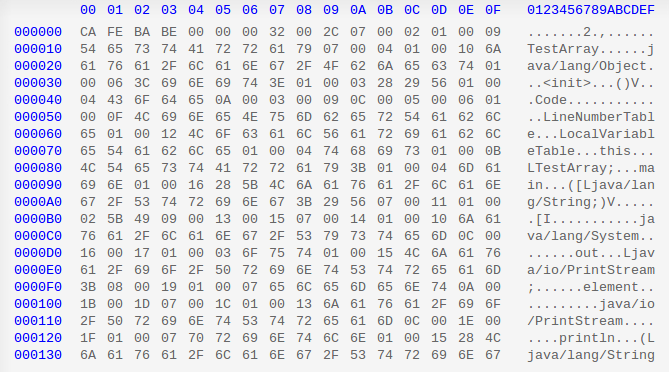
\includegraphics[width=0.85\textwidth]{images/java-bytecode-example.png}
	\caption{Java bytecode for the ``Hello World" code.}
	\label{fig:ch8:bytecode}
\end{figure}

%In Java that transformation is referred to as compilation. When Java code is compiled, a program called a compiler takes the Java code as input and as output produces code that’s easier for a computer to execute directly. \\

For instance, suppose that you have a text file with a large number of itemized expenses and you want to calculate the total cost of the expenses. To do this calculation, you could use a programming language to write code that instructs the computer to add up all of the expenses. This is more efficient than directly writing operations that the computer’s hardware can execute. \\ 

\section{Most popular programming languages}

Different programming languages are better for different applications. For example, some languages are better for making websites, while other languages are better for making mobile applications. \\

Java is one of the most popular programming languages. Java is used extensively by large companies like Oracle and Amazon. Java is also one of the primarily languages used to develop applications for the Android mobile operating system. \\

JavaScript is another very popular language. Despite its similarity to Java in name, JavaScript is a very different language from Java. JavaScript is one of the primary languages used for writing code to interact with browsers in websites, like Facebook or Google. 
%Javascript powers features of websites like generating dynamic content, sending requests to a server, making sure that the information entered in forms is correct, and many more things. 
%It’s also increasingly used to write applications. 
Javascript is a popular choice among newer and smaller companies. \\

Other programming languages that you might hear the names of include:
\begin{itemize}
\item \emph{Python}, \emph{Matlab}, and \emph{R}, three languages often used for scientific computing (e.g. mathematical modeling),
\item \emph{HTML} and \emph{CSS}, two languages used for writing websites,
\item \emph{C++}, one of the oldest/most common languages,
\item \emph{Assembly}, \emph{COBOL}, and \emph{Fortran}, three older languages that are behind a lot of old software (e.g. government software).
\end{itemize} 

The number and diversity of programming languages can be intimidating, but learning new programming languages becomes easier once you have a solid understanding of fundamental concepts. 
% We recommend focusing on one programming language initially to learn fundamental concepts rather than spending time trying to learn multiple languages. \\

In this course we use one programming language, Java, to teach these fundamental concepts.
However, the ideas and concepts you learn will help you learn any programming language you need to. 
We use Java because it’s easier to learn, widely used, and illustrates many important concepts in programming. 40\% of software developers stated that they know Java! \\

\section{Overview of GUI and Command Line}

The two primary ways to interact with your computer are to either use a (1) Graphical User Interface (GUI), or (2) command line.

A \textbf{Graphical User Interface (GUI)} is the primary way most users of a computer interact with the computer. For example, the file explorer (Figure \ref{fig:windows:file}) is a GUI that provides an easy way for users to complete tasks on their computer. It is popular because users can use their mouse and intuitive commands to complete basic tasks. \\

\begin{figure}
	\centering
	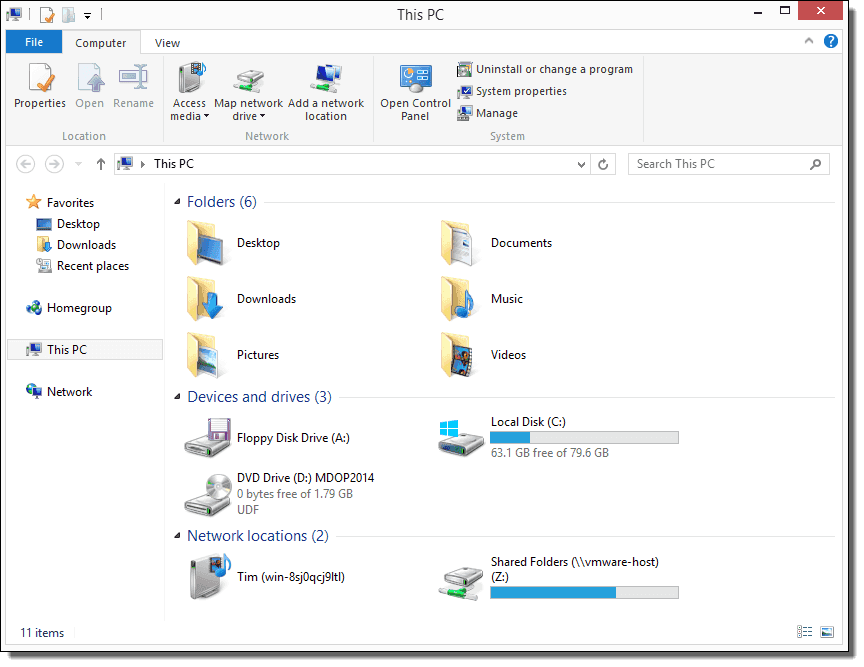
\includegraphics[width=0.85\textwidth]{images/windowsGUI.png}
	\caption{Windows file explorer}
	\label{fig:windows:file}
\end{figure}

The file explorer GUI hides the details of the operations being done by the computer away from the user of the program. This provides simplicity, but it also limits the flexibility of what a user can do with the computer. Moreover, it means that users can only interact with a system that has a GUI installed. This doesn’t include computers without a standard operating system, servers, or computers that a user is connected to remotely. \\

%The \textbf{command line} is a program you can access through the GUI of a linux machine. 
On the other hand, the \textbf{command line} is a program that  interface directly with the operating system and issue commands that it can understand. The command line can be accessed directly through the monitor without a GUI. In fact, before the invention of the GUI, the command line was the only way to interact with computers!  
%On modern computers, the command line can be accessed through the GUI of a linux machine. \\
%The command line is also installed on servers without a GUI and can be accessed directly through monitors (this was the only way to interact with computers before the invention of the GUI).\\

The command line allows the user to issue a broader range of commands and interact with computers without a graphical interface. 
%The command line lets users interface directly with the operating system and issue commands that it can understand. 
This increases the range of the commands that the user can issue, giving them more flexibility to perform complex and custom tasks. \\

\section{Linux command line}

We will discuss the command line used in the Linux operating system because it is one of the most common and intuitive command lines. \\

\begin{center}
    \begin{tabular}{| l | p{75mm} | }
      \hline
      Command & Description \\ \hline
      ls & List all the files in the current directory \\ \hline
      touch & Create a new file \\ \hline
      cd [name] & Changes the current directory to [name] \\ \hline
      mkdir [name] & Create a new directory within the current directory named [name] \\ \hline
      man [command] & Display the manual for a [command] \\ \hline
      cat [file] & Display the contents of [file] in the terminal \\ \hline
      mv [file] [location] & Moves [file] to the directory [location]. \\ \hline 
%      By default it moves file to a different name within the same directory. \\ \hline
      cp [file] [location] & Creates a new file with identical contents to the [file] specified in a new [location]. If a path for the file isn’t given, it will make a copy of the file in the same directory. \\ \hline
      rm [file] & Removes [file]. To remove a folder, use the command``rm -r [file]". \\ \hline
    \end{tabular}
\end{center}
  
  A folder in Linux is referred to as a \textbf{directory}. When you open a command line, you are located in a certain directory within the file system. All commands that you issue that relate to interacting with the file system like creating files, editing files, or renaming files will be issued in the context of this directory. This is like navigating to a particular folder within the GUI file explorer and completing all your operations relative to that folder.

\begin{figure}
	\centering
	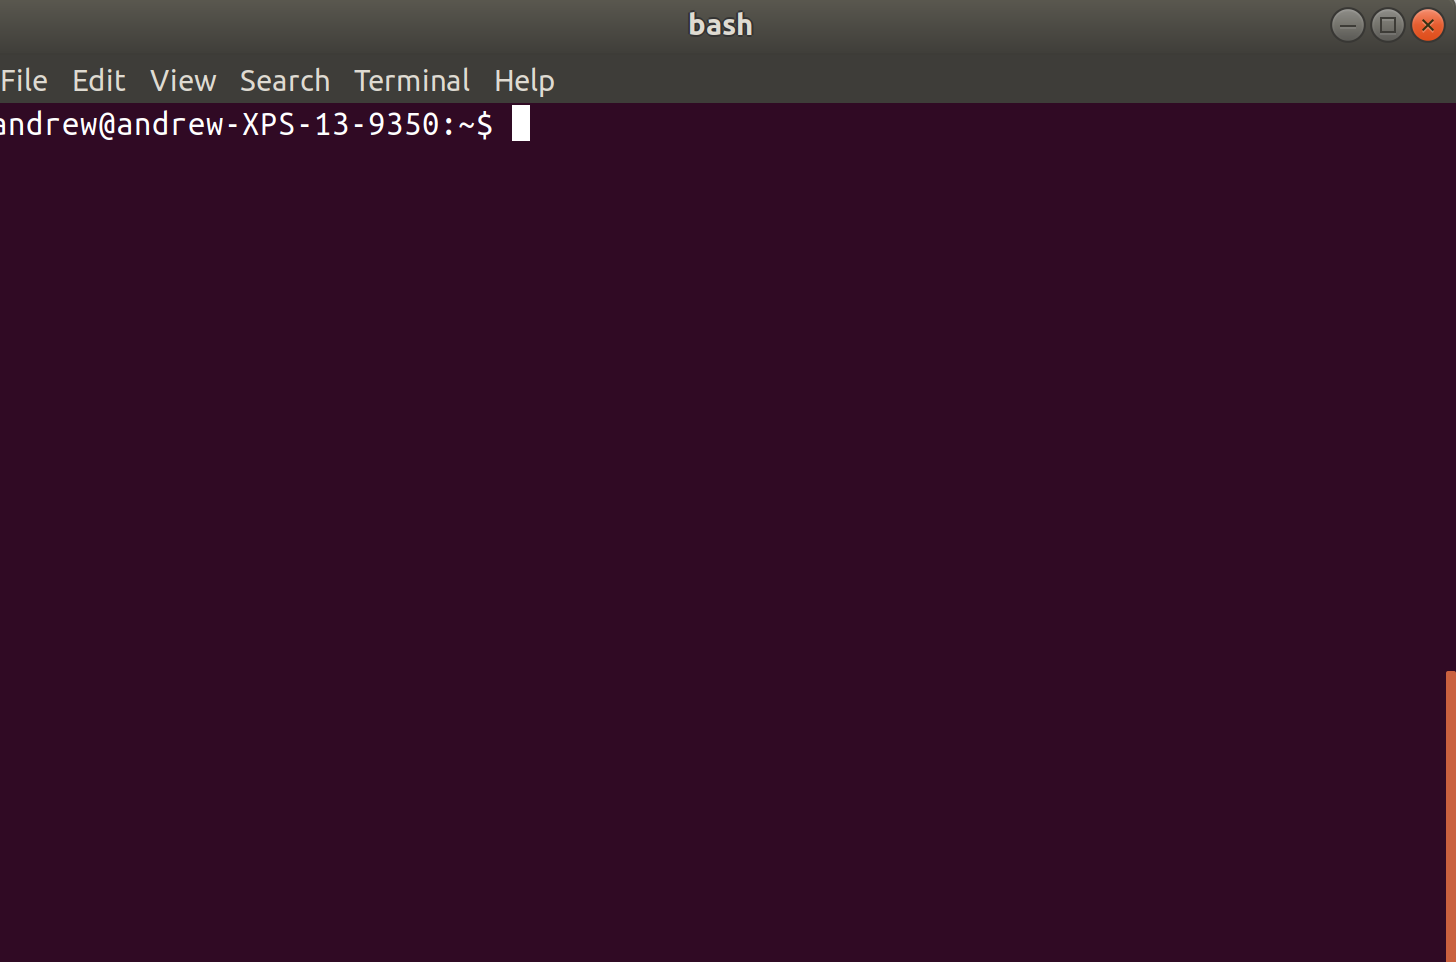
\includegraphics[width=0.85\textwidth]{images/commandLineOne.png}
	\caption{Linux command line}
	\label{fig:linux:one}
\end{figure}

Figure \ref{fig:linux:one} shows the command line interface for a Linux computer. The prompt shown is where the user can type commands. By default it prepends the user’s name, the name of the computer, and a dollar sign. The white rectangle represents the location of my cursor prompting the user to enter commands. \\

For example, Figure \ref{fig:linux:two} displays an example of creating a new directory called commandLineLearning (using the `mkdir` command) and then going inside the commandLineLearning directory (using the `cd` command). This is like making a new folder within an existing folder in the window’s file explorer, and then going inside that folder. \\

In Figure \ref{fig:linux:two}, the $\sim$ sign prepending the command represents the user’s home directory. The home directory is the outermost folder for that user’s account on the server or machine. \\

\begin{figure}
	\centering
	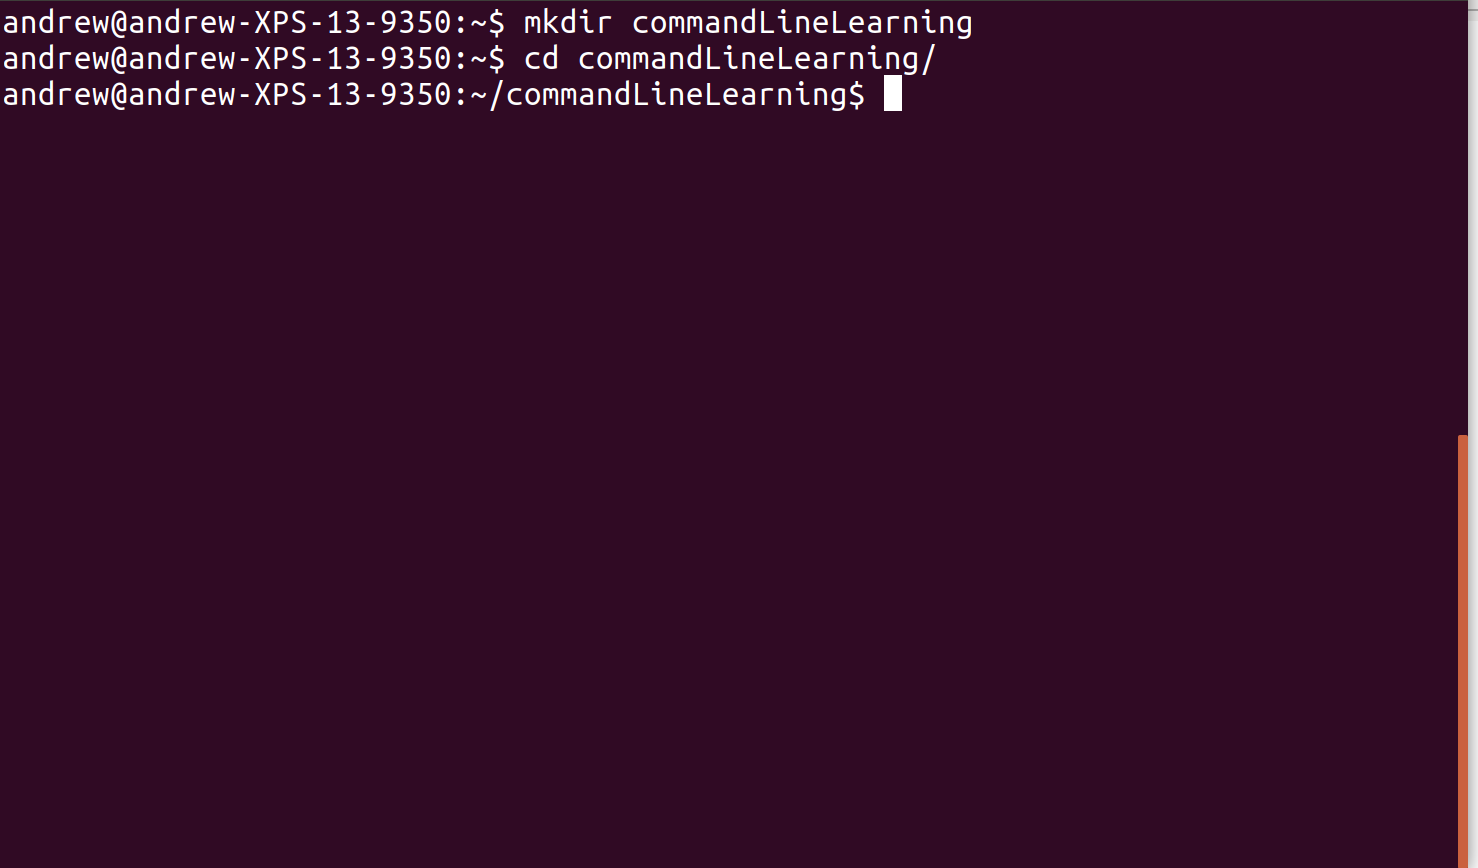
\includegraphics[width=0.85\textwidth]{images/commandLineTwo.png}
	\caption{Creating a directory}
	\label{fig:linux:two}
\end{figure}

\begin{figure}
	\centering
	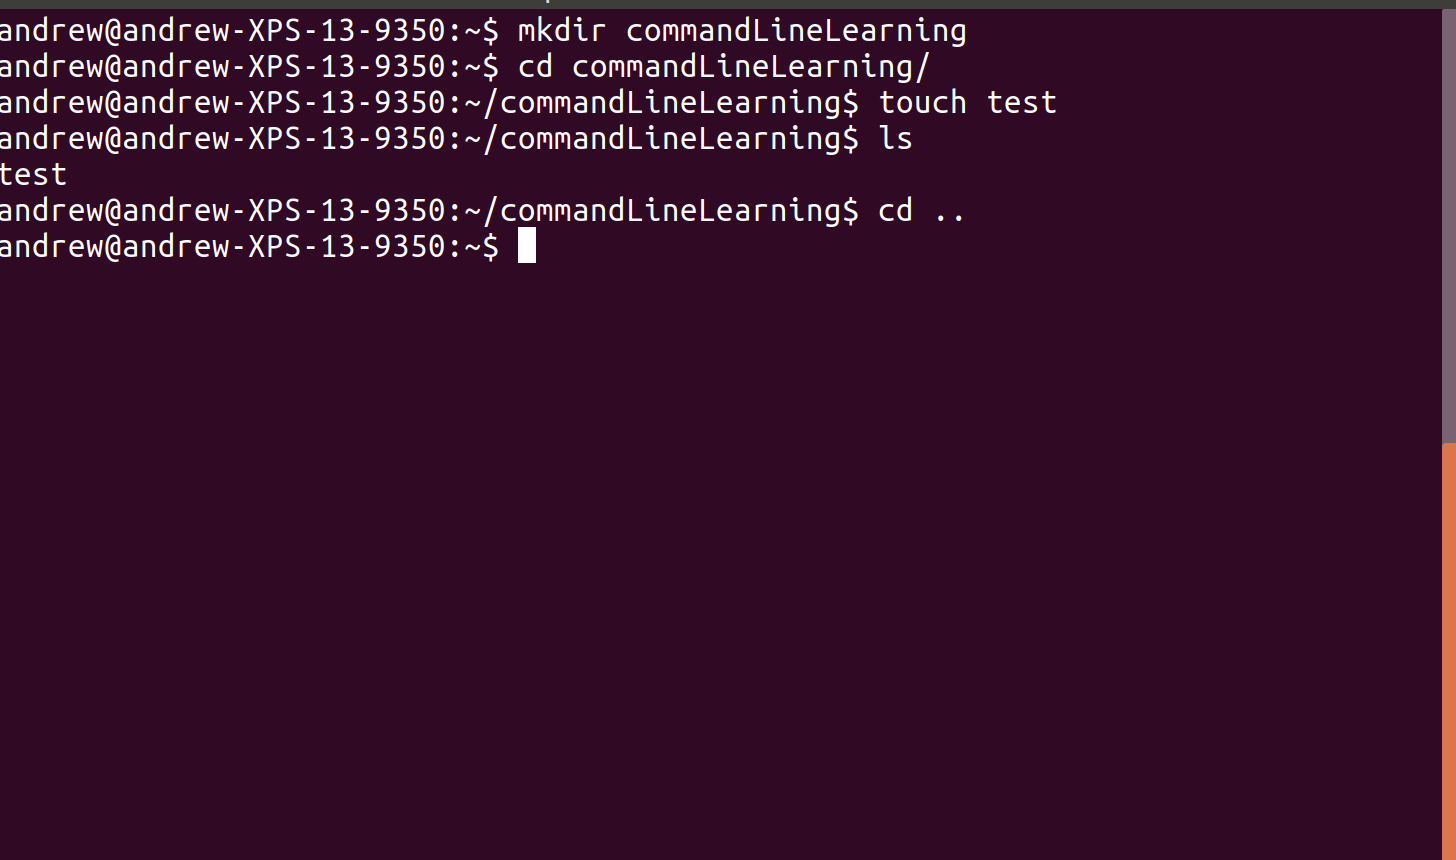
\includegraphics[width=0.85\textwidth]{images/commandLineThree.png}
	\caption{Listing files and navigating}
	\label{fig:linux:three}
\end{figure}

\begin{figure}[ht]
	\centering
	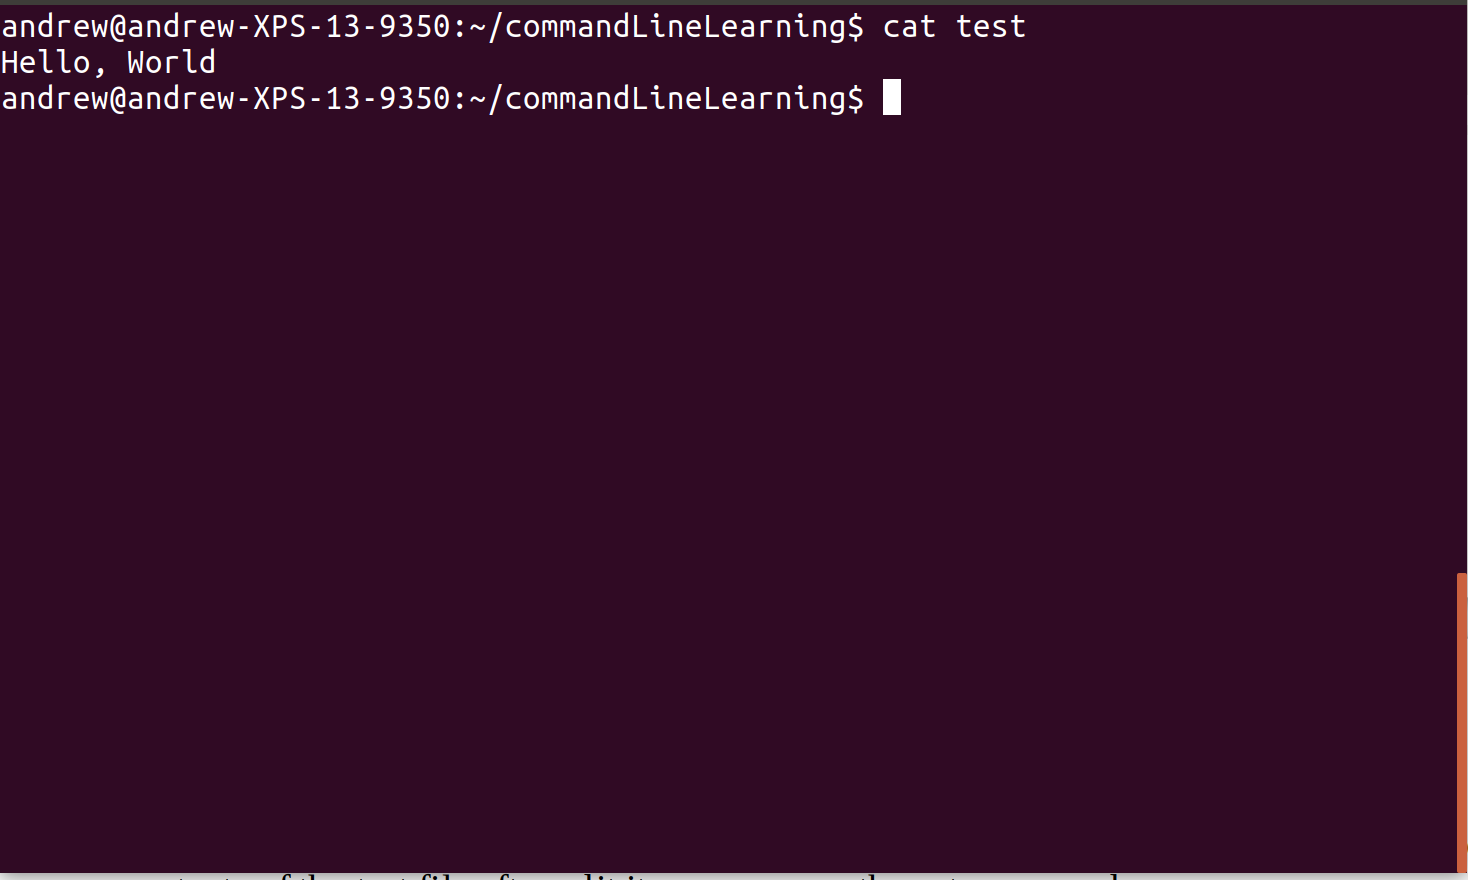
\includegraphics[width=0.85\textwidth]{images/commandLineFour.png}
	\caption{Cat command example}
	\label{fig:linux:four}
\end{figure}

If we want to create a file inside the commandLineLearning directory, we can use the ‘touch’ command to create a new file. If we want to see the files in the directory, we can use the ‘ls’ command to list all of the files inside the current directory. Finally, if we want to move back to the directory we were in before, we can use the ‘cd’ command with the parameters ‘..’ to move to the directory my current directory is contained within. In Linux, ‘..’ refers to the directory that contains the current directory, or the parent directory. These commands are summarized in Figure \ref{fig:linux:three}. \\

Try these commands out! You can edit the contents of test using any file editing software. To view the contents of the test file after you edit it, you can use the `cat` command (Figure \ref{fig:linux:four}). \\

%\newpage

\section{Lab: Running Hello World in the Command Line}

In this exercise, we will create a ``Hello World'' program in Java and run it --- only using the command line.

\begin{enumerate}
\item 
First, open the command line. 
\item Run the command \codeblock{cd $\sim$} which will move you to inside the \codeblock{$\sim$} folder. The \codeblock{$\sim$}  folder refers to your home directory.
\item
Next run \codeblock{cd Desktop}. This will take you to your Desktop. Afterwards, run \codeblock{cd CS103}, which will take you to your CS103 folder from Chapter 2. See Figure \ref{fig:linux:exercise:zero2}.

After running these commands, you might notice that the left side of your window (before the \$ sign) changes. This is because it indicates your current directory, which has changed from \codeblock{Desktop} to \codeblock{CS103}.

\begin{figure}[ht]
	\centering
	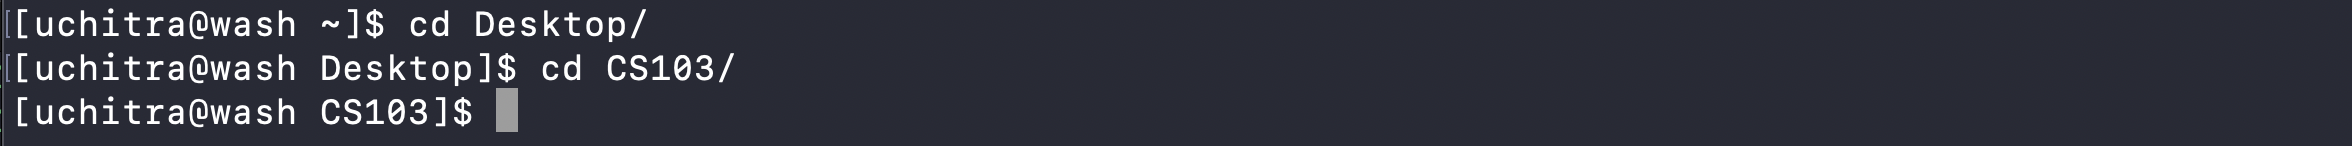
\includegraphics[width=0.85\textwidth]{images/commandLineExercise_zero2}
	\caption{Navigating to the \codeblock{CS103} folder you created from Chapter 2.}
	\label{fig:linux:exercise:zero2}
\end{figure}

\item
Next, run \codeblock{mkdir Chapter\_8}. This will create a folder called \codeblock{Chapter\_8} inside the \codeblock{CS103} folder. 

To check that you created this folder, run \codeblock{ls}. This will show all of the contents in your current folder. Verify that \codeblock{Chapter\_8} is listed. See Figure \ref{fig:linux:exercise:one2}.

\begin{figure}[ht]
	\centering
	
\includegraphics[width=0.85\textwidth]{images/commandLineExercise_one2}
	\caption{Creating and going inside the \codeblock{Chapter\_8} folder.}
	\label{fig:linux:exercise:one2}
\end{figure}

\item 
Then run \codeblock{cd Chapter\_8}. This will take you inside the \codeblock{Chapter\_8} folder.

\item
Next, we will copy the Hello World file we created in Chapter 2 into the \codeblock{Chapter\_8} folder we just created.

To do this, run the command 

\codeblock{cp ~/Desktop/CS103/Chapter\_2/HelloWorld.java ~/Desktop/CS103/Chapter\_8/}

To understand why this command works, recall that running \codeblock{cp [file] [location]} makes a copy of \codeblock{[file]} in \codeblock{[location]}. In the cp command above, \codeblock{[file]} is the path to the Hello World file from Chapter 2, and \codeblock{[location]} is the \codeblock{Chapter\_8} folder you just created.

To check that the \codeblock{cp} command worked successfully, run the \codeblock{ls} command. This will display all of the files in your current folder, which is the \codeblock{Chapter\_8} folder. You should see a file called \codeblock{HelloWorld.java}. See Figure \ref{fig:linux:exercise:two2}.

\begin{figure}[ht]
	\centering
	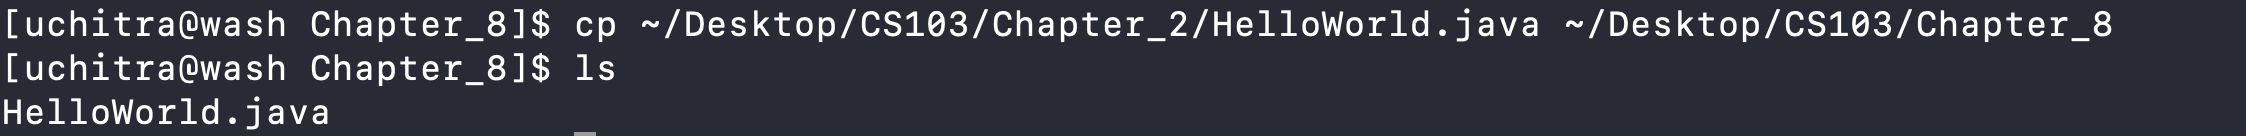
\includegraphics[width=0.85\textwidth]{images/commandLineExercise_two2}
	\caption{Copying the HelloWorld.java file from Chapter 2 into your \codeblock{Chapter\_8} folder.}
	\label{fig:linux:exercise:two2}
\end{figure}

\item
To verify that your code matches what you wrote in Chapter 2, run \codeblock{cat HelloWorld.java}. This will print out the contents of \codeblock{HelloWorld.java}.  See Figure \ref{fig:linux:exercise:three2}.

\begin{figure}[ht]
	\centering
	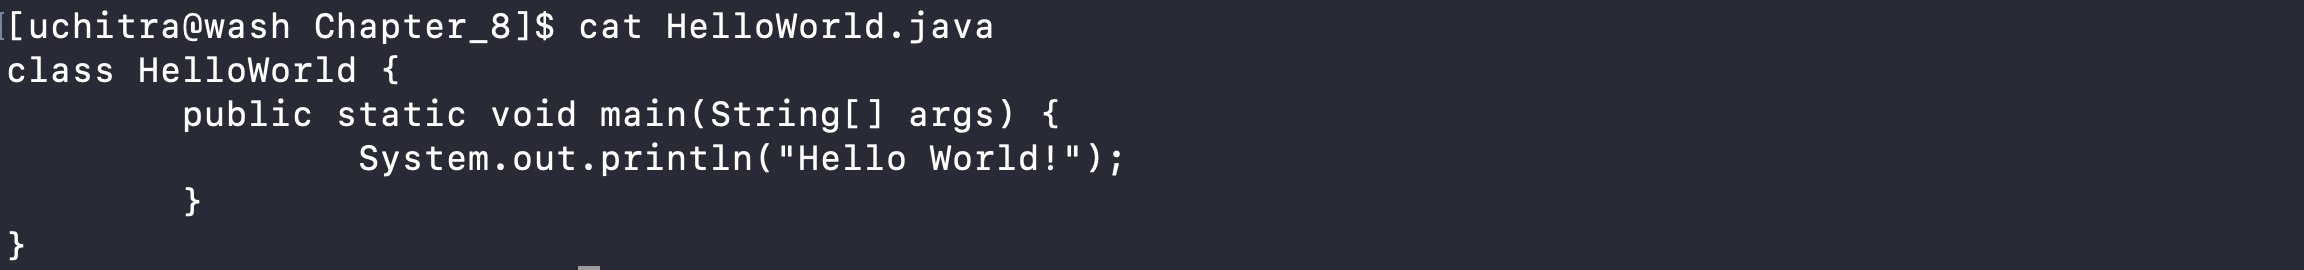
\includegraphics[width=0.85\textwidth]{images/commandLineExercise_three2}
	\caption{Running \codeblock{cat HelloWorld.java} to see the contents of \codeblock{HelloWorld.java}. Your code may look different depending on what you did in Chapter 2.}
	\label{fig:linux:exercise:three2}
\end{figure}

\item Now let's run our Hello World code! First, we have to compile the java file by running \codeblock{javac HelloWorld.java}. This will create a file named \codeblock{HelloWorld.class}. This file contains the bytecode instructions for the computer to run our program. See Figure \ref{fig:linux:exercise:four2}.

\begin{figure}[ht]
	\centering
	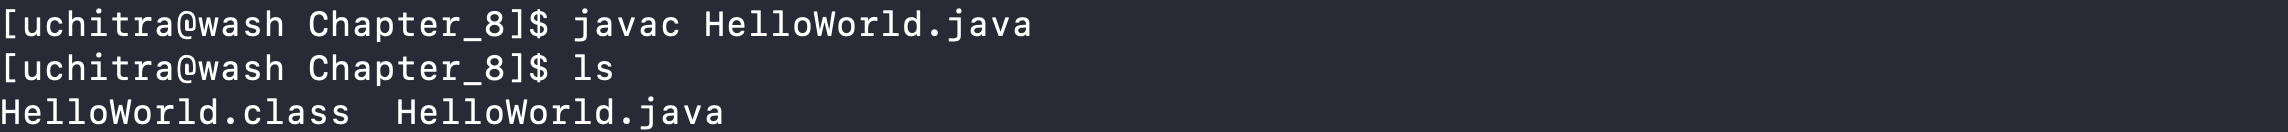
\includegraphics[width=0.85\textwidth]{images/commandLineExercise_four2}
	\caption{Running \codeblock{javac HelloWorld.java}. Running \codeblock{ls} afterwards shows that a \codeblock{HelloWorld.class} file was created.}
	\label{fig:linux:exercise:four2}
\end{figure}

\item Next, run \codeblock{java HelloWorld}. Here, the \codeblock{HelloWorld} refers to the name of the ``class" in the java file. If everything is correct, the result should be the phrase ``Hello World!", as shown in Figure \ref{fig:linux:exercise:five2}.

\begin{figure}[ht]
	\centering
	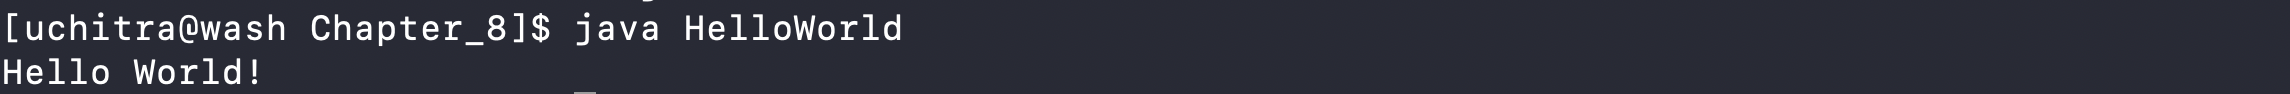
\includegraphics[width=0.85\textwidth]{images/commandLineExercise_five2}
	\caption{Running \codeblock{java HelloWorld.java}. The output of our program, which prints ``Hello World!", should appear below.}
	\label{fig:linux:exercise:five2}
\end{figure}

\item Congrats! You finished the lab! If you have extra time, check if someone sitting nearby needs any help.

\end{enumerate}
\newpage
\exercisesection

\begin{exercise}
Name three different programming languages.
\end{exercise}

\begin{exercise}
Name the process that turns your code into instructions that a computer can execute.
\end{exercise}

\begin{exercise}
Name an example of a GUI.
\end{exercise}

\begin{exercise}
Which command in the command line lets you to create a new directory?
\end{exercise}

\begin{exercise}
Which command in the command line lets you view the contents of a file?
\end{exercise}

\referencessection

Stack Overflow Developer Survey 2019. (n.d.).
    
	\chapter{Types and Variables}

We have seen a program that can print a simple ``Hello World'' message to the screen. Next we will learn about basic types of data that can be used in a Java program to perform calculations.

In this chapter, we will first learn about different types of data, focusing on five Java data types: \ic{int}, \ic{double}, \ic{boolean}, \ic{char}, and \ic{String}. Then we will learn about arithmetic, comparison, and logical operators over those types. Finally, we will learn about variables.

\section{Data types}
We work with different types of data all of the time: numbers, text, images, true/false or yes/no information, etc. Since we interact with numbers all the time, we can categorize numeric data in two ways: as (1) integers, which are whole numbers, or as (2) floating point numbers, which are numbers with digits after a decimal point or a fractional component.

Imagine the data you would find on a report card. It would probably have a lot of textual data, such as the student's name and their course names. It would probably also have a lot of numeric data, such as their age or their GPA. \ref{table:report_card} lists examples of information one might find on a report card.

\begin{table}[h!]
\centering
\begin{tabular}{ |c|c|c| }
 \hline
 Item & Example & Type of data \\
 \hline
 \hline
 Student name & John Doe & Text \\
 Course name & Honors Physics & Text \\
 Age & 17 & Integer (whole number) \\
 GPA & 3.75 & Floating point number\\
 \hline
\end{tabular}
\caption{Examples of pieces and types of data typically found on a report card.}
\label{table:report_card}
\end{table}

Now imagine an ice cream menu. It might have pictures of different flavors, along with the names of each flavor. It would probably list prices for different sizes and cones. It might also contain yes/no information, such as whether or not a certain flavor is dairy-free. \autoref{table:ice_cream_menu} lists examples of information one might find on such a menu.

\begin{table}[h!]
\centering
\begin{tabular}{ |c|c|c| }
 \hline
 Item & Example & Type of data \\
 \hline
 \hline
 Ice cream flavor & Mint Chocolate Chip & Text \\
 Price & \$3.99 & Floating point number \\
 Dietary information & Dairy-free & Yes/no \\
 \hline
\end{tabular}
\caption{Examples of pieces and types of data typically found on a menu at an ice cream shop.}
\label{table:ice_cream_menu}
\end{table}

\begin{example}
Take a look at the New Jersey driver's license in \autoref{fig:drivers_license}. List examples of different types of data you can find on it. \\

\noindent \emph{Answer}: Text (name, address), integers (date of birth, height, license number), yes/no (organ donor status).
\end{example}

\begin{figure}[h!]
  \centering
  
\includegraphics[width=0.5\textwidth]{images/nj_drivers_license}
  \caption{An example of a New Jersey driver's license. TODO: reference \href{https://www.state.nj.us/mvc/images/vetdefig.jpg}{the NJ state website (link here).}}
  \label{fig:drivers_license}
\end{figure}

We are surrounded by different types of data every day. We intuitively understand that different types of data interact in different ways. For example, you can add up the prices of multiple flavors of ice cream, but you cannot divide a student's name by their GPA. The same is true of data types in a Java program.

\begin{definition}
A \emph{data type} is a set of values and a set of operations defined on them.
\end{definition}

In the following sections, we will learn how Java represents different types of data: numeric data, true/false or yes/no data, and textual data. Specifically, we will focus on five types: \ic{int}, \ic{double}, \ic{boolean}, \ic{char}, and \ic{String}.

\subsection{Numeric data}
Representing numbers on a computer requires physical memory. For this reason, Java has six possible types for numeric data: four integer types (\ic{byte}, \ic{short}, \ic{int}, \ic{long}) and two floating point types (\ic{float}, \ic{double}). Some of these types require more memory in order to represent larger numbers, while other types use much less memory and can only represent small numbers. \autoref{table:numeric_types} summarizes this tradeoff between memory storage and numeric range or precision.

\begin{table}[h!]
\centering
\begin{tabular}{ |c|c|p{4.5cm}|p{4.5cm}| }
 \hline
 Type & Storage & Minimum Value & Maximum Value \\
 \hline
 \hline
 \ic{byte} & 8 bits & -128 & 127 \\
 \hline
 \ic{short} & 16 bits & -32,768 & 32,767 \\
 \hline
 \ic{int} & 32 bits & -2,147,483,648 & 2,147,483,647 \\
 \hline
 \ic{long} & 64 bits & -9,223,372,036,854,775,808 & 9,223,372,036,854,775,807 \\
 \hline
    \ic{float} & 32 bits & Approximately $-3.4 \times 10^{38}$ with 7 significant digits & Approximately $3.4 \times 10^{38}$ with 7 significant digits \\
 \hline
    \ic{double} & 64 bits & Approximately $-1.7 \times 10^{308} with 15 significant digits$ & Approximately $1.7 \times 10^{308}$ with 15 significant digits \\
 \hline
\end{tabular}
\caption{Java's six primitive numeric data types along with their memory requirements, range, and precision.}
\label{table:numeric_types}
\end{table}

In this course, we will focus on two of these numeric types: \ic{int} for integers and \ic{double} and floating-point numbers. We use \ic{int}s frequently in Java programs because integers, or whole numbers, show up naturally in everyday life. We also use \ic{double}s frequently in Java programs because floating point numbers often show up naturally in scientific applications. A \ic{double} in Java can either be written as a number with a decimal point (e.g. \ic{3.1415} or \ic{4.0}) or using scientific notation (e.g. \ic{6.022e23}). The \ic{e} in this notation is shorthand for ``times 10 to the power of \_\_\_\_''. For example, \ic{6.022e23} is equivalent to $6.022 \times 10^{23}$.

\begin{example}
What are examples of integers in everyday life? \\

\noindent \emph{Answer}: Age (7), number of siblings (2), the result of a dice roll (5), approximate population in New Jersey (8,908,520)
\end{example}

\begin{example}
What are examples of floating point numbers in everyday life? \\

\noindent \emph{Answer}: GPA (4.0), price of a chocolate bar (\$1.99), balance in bank account (\$514.66), average rating out of 5 stars (4.5 out of 5).
\end{example}

\begin{example}
What is the value of \ic{1.23e3}? \\

\noindent \emph{Answer}: It is $1.23 \times 10^3 = 1.23 \times 1000 = 1230$.
\end{example}

\subsection{True/false data}
To represent true/false, yes/no, or on/off data, Java uses \ic{boolean}s. A \ic{boolean} can only be one of two possible values: \ic{true} or \ic{false}. For example, the statement ``The sky is blue right now'' can only either be true or false. If it is daytime, it is most likely true. If it is nighttime or if the sun is currently setting, then it is most likely false. Similarly the statement ``2 plus 2 equals 4'' is clearly true, so we can represent this as a \ic{boolean}. In the same way, we can see that ``3 times 4 is 11'' is false. \ic{boolean}s may seem simple, but we will see soon how to combine them in complex and powerful ways.

\subsection{Textual data}
In general, Java has two main types to represent textual data: a (1) \ic{char} for a single letter or symbol or a (2) \ic{String} for a sequence of multiple letters. A \ic{char} is a single alphanumeric character or symbol, like the ones you can type on your keyboard, that is expressed in Java using single quotes. \ic{'A'}, \ic{'z'}, and \ic{'\$'} are all examples of chars in Java. A \ic{String} is a sequence of characters that is expressed in Java using double quotes. \ic{``Hello World''} is an example of \ic{String}.

\begin{example}
Is \ic{'@'} a valid \ic{char}? \\

\noindent \emph{Answer}: Yes!
\end{example}

\begin{example}
Is \ic{``P''} a valid \ic{char}? \\

\noindent \emph{Answer}: No. A \ic{char} must use single quotes.
\end{example}

\begin{example}
Is \ic{'ABC'} a valid \ic{char}? \\

\noindent \emph{Answer}: No. A \ic{char} must only be a single character.
\end{example}

\begin{example}
What are some examples of \ic{String}s in everyday life? \\

\noindent \emph{Answer}: Text messages, names of friends, email addresses, a poem
\end{example}

\subsection{Summary of five types}
Java has many built-in data types for different types of data: numeric, true/false, and text. In this section, we have focused on five of these types: \ic{int} for integers, \ic{double} for floating point numbers, \ic{boolean} for true/false values, \ic{char} for single characters, and \ic{String} for a sequence of characters. \autoref{table:types_summary} summarizes these five types.

\begin{table}[h!]
\centering
\begin{tabular}{ |c|c|c| }
 \hline
 Type & Description & Examples \\
 \hline
 \hline
 \ic{int} & integers & 5, -100, 1,234,567 \\
 \hline
 \ic{double} & floating point number & 3.75, 6.022e23 \\
 \hline
 \ic{boolean} & true/false value & \ic{true}, \ic{false} \\
 \hline
 \ic{char} & characters & \ic{'A'}, \ic{'\%'}, \ic{'5'} \\
 \hline
 \ic{String} & sequences of characters & \ic{``Hello''}, \ic{``123 Happy St.''} \\
 \hline
\end{tabular}
\caption{A summary of five of Java's built-in types}
\label{table:types_summary}
\end{table}

\section{Operations}
Now that we have learned about data types, we will next learn about the operations we can perform on the the different data types. Specifically, we will learn about arithmetic and comparison operators used with numeric types (e.g. \ic{int}s and \ic{double}s). Then, we will discuss logical operators used with \ic{boolean}s. Finally, we will learn about operations we can perform on \ic{String}s.

\subsection{Arithmetic operators}
Arithmetic operators are generally the ones we are familiar with from elementary school, such as addition (\ic{+}), subtraction (\ic{-}), multiplication (\ic{*}), and division (\ic{/}). For example, \ic{5 + 3} equals \ic{8}, \ic{5.55 - 1.11} equals \ic{4.44}, and \ic{1.5 * 10} equals \ic{15}. Note that just like in regular math, the operator \ic{-} can also refer to negation of the number it's written before. Therefore, \ic{-3} is a correct expression, as well as \ic{5 + -3}, which equals 2.

Of these basic arithmetic operators, division is the trickiest because it behaves in a special way with integers. In Java, if you were to divide two integers, you would get an integer as a result. This is intuitive in some cases. For example, \ic{20 / 5} would equal \ic{4}. However, in other cases, we may lose a fractional component. For instance, \ic{21 / 5} also equals \ic{4}. You might think that \ic{21 / 5} should equal \ic{4.2}, but the fractional piece (everything after the decimal point) gets \emph{truncated}, or dropped completely. This is what we call \emph{integer truncation}. It is worth nothing that truncation is different than \emph{rounding}: as a simple example, rounding would cause 3.9 to become 4, whereas truncating would cause 3.9 to become 3.

\begin{example}
What is \ic{2 / 2}? What about \ic{3 / 2}? What about \ic{4 / 2}? \\

\noindent \emph{Answer}: \ic{2 / 2} equals {1}. \\
\ic{3 / 2} also equals {1} (after dropping the \ic{.5} from the answer \ic{1.5}). \\
\ic{4 / 2} equals {2}.
\end{example}

Java also has an extra arithmetic operator, called the ``modulo'' operator (or ``mod'' for short), that looks like a percent symbol \ic{\%}. Its purpose is to compute the remainder when dividing two numbers. For example, \ic{13 \% 3}, which we pronounce as ``thirteen mod three'', is equal to \ic{1} because 13 divided by 3 gives us 4, remainder 1.

\begin{example}
What is \ic{15 \% 10}? What about \ic{6.25 \% 3}? \\

\noindent \emph{Answer}: \ic{15 \% 10} equals \ic{5}. \\
\ic{6.25 \% 3} equals \ic{0.25}.
\end{example}

In addition to these five arithmetic operators, Java also provides additional mathematical functions that you might find on a basic scientific calculator, such as square root, absolute value, logarithms, etc. For example, \ic{Math.sqrt(25)} equals \ic{5} and \ic{Math.abs(-10)} equals \ic{10}. \autoref{table:math_functions} lists a few examples of mathematical functions provided by Java.

\begin{table}[h!]
\centering
\begin{tabular}{ |c|c|c| }
 \hline
 Function & Description & Example \\
 \hline
 \hline
 \ic{Math.abs(x)} & Absolute value of \ic{x} & \ic{Math.abs(-10)} equals \ic{10} \\
 \hline
 \ic{Math.pow(a, b)} & \ic{a} to the power of \ic{b} ($a^b$) & \ic{Math.pow(2, 3)} equals \ic{8} \\
 \hline
 \ic{Math.sqrt(x)} & Square root of \ic{x} & \ic{Math.sqrt(16)} equals \ic{4} \\
 \hline
\end{tabular}
\caption{A list of a few mathematical functions provided in Java}
\label{table:math_functions}
\end{table}

Of course, we can combine all of these arithmetic operators and mathematical functions in Java to perform complex computation. For example, we might write \ic{Math.sqrt(9) + (5 * 2) - Math.abs(-3)}. Just as you would on a calculator, you can use parentheses to indicate the order of operations in an expression.

\begin{example}
What is the result of \ic{Math.sqrt(9) + (5 * 2) - Math.abs(-3)}? \\

\noindent \emph{Answer}: \ic{Math.sqrt(9) + (5 * 2) - Math.abs(-3)} equals \ic{3 + 10 - 3} which is equal to \ic{10}.
\end{example}

\subsection{Comparison operators}
Comparison operators are operators that compare numeric data. You are probably familiar with the following comparison symbols from math class: $=, <, \leq, >$, and $\geq$. In Java, we use the symbols \ic{==}, \ic{!=}, \ic{<}, \ic{<=}, \ic{>}, \ic{>=}. The result of any comparison operation is a \ic{boolean}. For example, the result of \ic{5 >= 3} is \ic{true}. \autoref{table:comparison_ops} summarizes a list of these comparison operators along with examples.

\begin{table}[h!]
\centering
\begin{tabular}{ |c|c|c|c| }
 \hline
 Operator & Description & Example 1 & Example 2 \\
 \hline
 \hline
 \ic{==} & Equals & \ic{5 == 5} is \ic{true} & \ic{3 == 5} is \ic{false} \\
 \hline
 \ic{!=} & Not equal & \ic{5 != 5} is \ic{false} & \ic{3 != 5} is \ic{true} \\
 \hline
 \ic{<} & Less than & \ic{5 < 5} is \ic{false} & \ic{3 < 5} is \ic{true} \\
 \hline
 \ic{<=} & Less than or equal to & \ic{5 <= 5} is \ic{true} & \ic{3 <= 5} is \ic{true} \\
 \hline
 \ic{>} & Greater than & \ic{5 > 5} is \ic{false} & \ic{3 > 5} is \ic{false} \\
 \hline
 \ic{>=} & Greater than or equal to & \ic{5 >= 5} is \ic{true} & \ic{3 >= 5} is \ic{false} \\
 \hline
\end{tabular}
\caption{A list of the comparison operators, along with examples}
\label{table:comparison_ops}
\end{table}

\subsection{Logical operators}

Logical operators are used to manipulate boolean values. Like comparison operators, the result of an expression with logical operators is a boolean. The three most common logical operators in Java are \ic{\&\&} (logical And), \ic{||} (logical Or) and \ic{!} (logical Not). There are also other operators (|, \&, \^) that we will not cover. Finally, the equality and inequality operators (==, !=) can be applied on boolean values too.

The logical And takes two boolean values and returns true if and only if both values are true. To use it, write the operator between the values. For example, \ic{false \&\& true} applies And to false and true, and the result is false. The following table summarizes the values of And for every input:


\begin{table}[h!]
\centering
\begin{tabular}{ |c|c|c| }
 \hline
 A & B & \ic{And (A \&\& B)} \\
 \hline
 \hline
 false & false & false \\
 \hline
 false & true & false \\
 \hline
 true & false & false \\
 \hline
 true & true & true\\
 \hline
\end{tabular}
\caption{The truth table of And}
\label{table:And}
\end{table}

The logical Or takes two boolean values and returns true when at least one of them is true. Notice that, unlike its usage in language, Or is not exclusive - \ic{A || B} does not mean ``either A or B'' but ``at least one of the two - A, B''. The following table summarizes the values of Or for every input:


\begin{table}[h!]
\centering
\begin{tabular}{ |c|c|c| }
 \hline
 A & B & \ic{Or (A || B)} \\
 \hline
 \hline
 false & false & false \\
 \hline
 false & true & true \\
 \hline
 true & false & true \\
 \hline
 true & true & true\\
 \hline
\end{tabular}
\caption{The truth table of Or}
\label{table:Or}
\end{table}

The logical Not operates on one boolean value, and inverts it. It is written before the value, so for example \ic{!false} is equal to true. 

Like arithmetic and comparison operators, we can combine different logic operators, and even comparison operators, in the same expression.

\begin{example}
What is the result of \ic{(!(2 > 3)) || (0 == 1)}? \\

\noindent \emph{Answer}: \ic{2 > 3} is false. Therefore, \ic{!(2 > 3)} is true. Since at least one of \ic{!(2 > 3)}, \ic{0 == 1} is true, the whole expression is true.
\end{example}

\subsection{Operator Precedence}

We already saw that parentheses can be used to mark the order in which we want to apply operators. What happens, however, when we do not specify the order ourselves? For example, what is the value of \ic{2 > 3 || 0 == 1}? It turns out that in this case, the order of operation the Java language will choose is the same as for the expression \ic{(2 > 3) || (0 == 1)}. This is because some operators take precedence, and are computed before others. In this case, the first operator to be computed is \ic{>}, and it interprets its arguments as the nearest, 2 and 3. Then \ic{==} is executed, interpreting its arguments as 0 and 1. Only then \ic{||} is executed, and the arguments it recognizes are the results of the previous comparisons.

We will not cover the complete order of precedence (that also includes many operators not covered here), and the way ties are broken (for example, in \ic{A || B || C}). Important rules to remember are:

\begin{itemize}
\item Parentheses take precedence over any other operator.
\item Logical And takes precedence over logical Or. 
\item Multiplication takes precedence over addition.
\item Arithmetic operation take precedence over comparisons, which take precedence over logical operators.
\end{itemize}

When in doubt, use parentheses. Even if the result is the same, this can help a reader follow your code more easily. 


\subsection{\ic{String} methods}

Java has a set of operations we can use for building strings. The most common operation we will need is concatenation, or combining two strings. The same sign for the addition operator, +, is used to concatenate strings. For example, \ic{"Hello" + " " + "world"} will result in the string ``Hello world''. Notice that concatenation does not add a space between strings. If we want to concatenate two words, we need to explicitly write a space between them, as in the previous or following example: \ic{"Two " + "words"}.

Another common operation we would like to do with strings is to compare them. For example, check whether two strings are the same. The == operator works on strings as well, but it does not do what we expect. Instead, it checks whether the two strings reference the same object (we will learn about objects later in the course). Instead, when we want to compare two strings, we will use a method called "equals". If A and B represent two strings, we can ask whether they are equal in the following way: \ic{A.equals(B)}. Note that upper and lower case letters are considered different, and that spaces are also counted for comparisons.


\begin{example}
What is the result of \ic{"Room".equals("room")}? \\

\noindent \emph{Answer}: Since the first letter in the two strings differs, the result is false.
\end{example}


\begin{example}
What is the result of \ic{("one" + "two").equals("one two")}? \\

\noindent \emph{Answer}: The result of the concatenation is "onetwo". Since it does not have a space, it is unequal to "one two", and the result is false.
\end{example}

Strings are very common in programming, and so Java has many more string methods. We will learn about them later, as we start to write our own programs.

\section{Variables}
We have now seen data types and operators. So far, we have only worked with \emph{literals}, meaning we have given \emph{literal} examples of values of data types, such as \ic{5} for \ic{int}s or \ic{``Hello World''} for \ic{String}s.

\begin{definition}
A \emph{literal} is an explicit data value used in a program.
\end{definition}

Sometimes, however, we might want to use a \emph{placeholder} to refer to an item of data. This often allows our Java programs to be more general. For example, instead of typing \ic{``John Doe''} literally in our program, we might use \ic{fullname} as a \emph{variable}, or a placeholder, to refer to a person's name on a document.

\begin{definition}
A \emph{variable} is a name for a location in memory used to hold a data value.
\end{definition}

\noindent To create and use a variable, we typically need to do three main things:
\begin{enumerate}
 \item Choose what type of data it will represent (e.g. \ic{int} or \ic{boolean})
 \item Choose what we want to call it (e.g. \ic{name} or \ic{fullname} or \ic{person})
 \item Store a value into the variable (e.g \ic{``John Doe''} or \ic{``Mary Jane''})
\end{enumerate}
We can accomplish these three tasks in two main steps: \emph{declaration} and \emph{assignment}.

\begin{definition}
A \emph{declaration statement} (1) reserves a portion of memory space large enough to hold a particular type of value and (2) indicates the name by which we refer to that location.
\end{definition}

\noindent Examples of declaration statements include:
\begin{itemize}
 \item \ic{String name;}
 \item \ic{int age;}
 \item \ic{double gpa;}
 \item \ic{boolean isOrganDonor;}
\end{itemize}

\begin{definition}
An \emph{assignment statement} sets and/or resets the value stored in the storage location denoted by a variable name; in simpler terms, it stores, or \emph{assigns}, a value to a variable.
\end{definition}

\noindent Examples of assignment statements include:
\begin{itemize}
 \item \ic{name = "John Doe";}
 \item \ic{age = 17;}
 \item \ic{gpa = 3.75;}
 \item \ic{isOrganDonor = true;}
\end{itemize}
	Of course, the values you store into variables must match the type you declared them to be. Otherwise, you will encounter a compiler error. For example, \ic{int x = "x";} would lead to an error.	
In Java, you are allowed to combine a declaration statement and an assignment statement into a single line. For example, instead of a line \ic{String name;} followed by another line \ic{name = "John Doe";}, you can write a single line, \ic{String name = "John Doe";}.	
\begin{example}	
  What will the following code snippet print out?
    Here you should be aware that using ``System.out.print'' will print exactly what it is given and nothing more,
    whereas ``System.out.println'' will add a new line to the end, such that the next thing that gets printed will be on a new line.
  \begin{lstlisting}[language=Java]
public class Snippet{
    public static void main(String []args){
        String a = "computer  science ";	
        int b = 4;	
        String c = " ever";	
        System.out.print(a);	
        System.out.print(b);	
        System.out.print(c);	
        System.out.println();	
        c = " life";	
        System.out.print(a);	
        System.out.print(b);	
        System.out.print(c);	
        System.out.println();
    }
}
  \end{lstlisting}
  
  Try it by yourself by copying the code to DrJava!
\end{example}	
It is important to note the difference between the single equals sign used for assignment and the double equals sign used for comparison. In \ic{age = 17;} the single equals sign represents an \emph{assignment statement}, meaning we are storing the value 17 into a variable named \ic{age}. In contrast, in \ic{age == 17}, the double equals sign represents the fact that we are comparing the value of age to 17, meaning we are asking a yes/no question, whether or not \ic{age} is equal to 17. Look at the following code snippet and make sure you understand the difference between \ic{=} and \ic{==}.	
\begin{lstlisting}[language=Java]	
public class Snippet{
    public static void main(String []args){
        int a = 5;	
        int b = 3;	
        System.out.println(a == b);   // prints false	
        a = b;                        // now a is 3	
        System.out.println(a == b);   // prints true	
    }
}
\end{lstlisting}	
When using the \ic{=} symbol to assign to a variable, the variable you are assigning to should always go on the left. For example, we can write \ic{x = 5;} to assign \ic{5} to \ic{x}, but \ic{5 = x;} is not valid Java code, since we can't assign to a literal. If we have two different variables, say \ic{x} and \ic{y}, then \ic{x = y;} and \ic{y = x;} are both valid lines of code, but they do different things. If we write \ic{x = y;}, then the value of \ic{x} changes to become the value of \ic{y}. If we write \ic{y = x;}, then the value of \ic{y} changes to become the value of \ic{x}.	
\begin{example}	
  Fill in some code in the middle of the following snippet to swap the values of \texttt{a} and \texttt{b}. The code should print \ic{ABBA} if you do this correctly. \emph{Hint:} you may need to define a third variable!	
  \begin{lstlisting}[language=Java]	
public class Snippet{
    public static void main(String []args){
        String a = "A";	
        String b = "B";	
        System.out.print(a);	
        System.out.print(b);	
        // Your code here	
        // Swap the values of a and b	
        System.out.print(a);	
        System.out.println(b);	
    }
}
  \end{lstlisting}	
\end{example}	
A declaration statement will also lead to a compiler error if the variable has already been declared. For example, if we have a line \ic{int x = 5;} followed by another line \ic{int x = 7;}, the compiler will see the second line and complain that the variable \ic{x} has already been declared. You might imagine that this could cause some difficulties: in a large program, we might want to use the variable \ic{x} to mean different things at different points, without worrying about whether \ic{x} has been declared earlier. Luckily, Java and most other programming languages provide a tool to manage this, called \emph{scope}.	
\begin{definition}	
  The \emph{scope} of a variable is the section of code where it can be referenced.	
\end{definition}	
In all of the examples we have seen so far, the scope of a variable consists of all lines after the declaration statement for that variable. In later lectures, we will see how more advanced tools can restrict the scope of variables.	
Previously we saw that we can combine multiple operations with literals to perform more complex computation. In the same way, we can combine literals and variables and operators altogether.	
\begin{definition}	
An \emph{expression} is a combination of one or more operators and operands that usually performs a calculation.	
\end{definition}	
For example, look at the following code snippet for computing the area of a circle.	
\begin{lstlisting}[language=Java]	
public class Snippet{
    public static void main(String []args){
        double radius = 4.5;	
        double area = 3.14*radius*radius;	
        System.out.print("Radius: ");	
        System.out.println(radius);	
        System.out.print("Area: ");	
        System.out.println(area);	
    }
}
\end{lstlisting}	
We can even update the value of a variable with an expression that includes that same variable. For example, \ic{x = x + 5;} will increase the value of \ic{x} by 5.	
\begin{example}	
  To convert from Celsius to Fahrenheit, multiply by 1.8 and then add 32. Fill in a single line of code below to convert \ic{temp} from Celsius to Fahrenheit;	
  \begin{lstlisting}[language=Java]	
public class Snippet{
    public static void main(String []args){
        double temp = 12;	
        System.out.print("The temperature is ");	
        System.out.print(temp);	
        System.out.println(" degrees Celsius");	
        // Your code here	
        System.out.print("The temperature is ");	
        System.out.print(temp);	
        System.out.println(" degrees Fahrenheit");	
    }
}
  \end{lstlisting}	
\end{example}	
There are a few shorthand notations for updating variables. If you want to act on a variable \ic{var} with a single operator, such as \ic{var = var - 7;} or \ic{var = var * 2.3;}, you can abbreviate this as \ic{var -= 7;} or \ic{var *= 2.3} respectively. This works for any of the arithmetic operators: you can use \ic{+=}, \ic{-=}, \ic{*=}, \ic{/=}, or \ic{\%=}.	
When mixing variables in expressions, it is important to be aware of their types and to know how variables of different types combine together. When working with numeric types, if you combine two values of the same type with an operator, the result will also be of that type. A common pitfall for this rule is division: if you divide two \ic{int}s, the result will be an \ic{int}.	
\begin{lstlisting}[language=Java]
public class Snippet{
    public static void main(String []args){
        int x = 8;	
        int y = 5;	
        System.out.println(x/y); // prints 1
    }
}
\end{lstlisting}	
Even though 8/5 = 1.6, Java will interpret \ic{x/y} as another \ic{int}, so it becomes \ic{1}. This is just like dividing integer literals, but with variables, you have to keep in mind what the variable types are so you will know if division will be truncated.	
When you combine two different numeric types, the result will be a value of the more precise type. The most common example of this is combining an \ic{int} with a \ic{double}, which will result in a \ic{double}. This is called "automatic type conversion".
You can also override Java's default rules for assigning types to expressions by using \emph{casting}. Casting allows you to tell Java to interpret an expression as a given type by putting the desired type in front of the expression in parentheses: for example, \ic{(int) x} casts \ic{x} to an \ic{int}. For now, we will only use casting to convert between different numeric types. Later on we will learn more detailed rules for casting.	
\begin{example}	
  Look at the following examples and make sure you understand how Java assigns a type to each expression. Keep track of the parentheses so you know what is being casted.	
  \begin{lstlisting}[language=Java]	
public class Snippet{
    public static void main(String []args){
        double eight = 8.0;	
        int five = 5;	
        System.out.println(eight/five); // prints 1.6	
        System.out.println((int)(eight/five)); // prints 1	
        System.out.println(eight/((double)five)); // prints 1.6	
        System.out.println(((int) eight)/five); // prints 1	
        System.out.println(((int) eight)/((double) five)); // prints 1.6
    }
}
  \end{lstlisting}	
\end{example}	

As previously mentioned, Java will attempt ``automatic type conversion" in case you try to assign a lower-precision value to a type that has higher precision without casting yourself. Java will throw an error, however, if you try to assign a higher-precision value to a lower-precision type. This can get very confusing. So it's best to avoid type conversion in your code when you can, and explicitly cast the type when you must. 

\begin{example}
  What will happen if you compile and run this code? 
  \begin{lstlisting}[language=Java]
public class Snippet{
    public static void main(String []args){
        int intEight = 8;
        double doubleEight = intEight;
        System.out.println(doubleEight);
    }
}
  \end{lstlisting}
  
  How about this code? 
  \begin{lstlisting}[language=Java]
public class Snippet{
    public static void main(String []args){
        double doubleEight = 8.0;
        int intEight = doubleEight; 
        System.out.println(intEight);
    }
}
  \end{lstlisting}
  
\noindent \emph{Answer}: In the first example, Java will happily use automatic type conversion to convert the lower-precision int (intEight) to the higher-precision double (doubleEight). The output of the code is \ic{8.0}, the double version of \ic{8}. In the second example, however, Java cannot use automatic type conversion to go from a higher-precision double (doubleEight) to a lower-precision int (intEight). Java will throw an error when you try to compile this code. 
\end{example}

\subsection{Variable names}

There are some rules variable names need to follow (with some exceptions omitted):

\begin{itemize}
\item A variable name must begin with a letter.
\item The digits 0--9 and the character \_ can appear in a variable name, as long as it does not begins with them. 	
\item Spaces and other special characters (like \%, \#, and \textasciicircum) cannot appear in a variable name.	
\item A keyword used for the Java language itself cannot be used as a variable name (for example, \ic{String}).	
\end{itemize}	
Lower- and upper-case letters are considered different in variable names, and so \ic{name} and \ic{Name} are considered different names. There are naming conventions for variables, that help us read code easily and understand what the function of each variable is:	
\begin{itemize}	
\item Variables should have short, meaningful names. Limit variable names to a few short words, and make sure that a reader unfamiliar with the code could easily understand what the purpose of each variable is. 	
\item Most variable names should start with a lower-case letter, and each new word after the first should start with an upper-case letter (for example, \ic{firstName}). This naming pattern is called camel case, and is used for many other languages.	
\item Constant variables, whose value should not change, should be written with all caps (upper-case letters), and different words should be separated by an underscore (for example, \ic{MAXIMAL\_WEIGHT}).	
\item Temporary variables, that are only used for a short part of the code, can have single letter names. Typically, \ic{i}, \ic{j}, \ic{k}, \ic{m} and \ic{n} are used for integer values, and \ic{c}, \ic{d} and \ic{e} for characters.
\end{itemize}

Programming is often a collaborative process, in which different people work on the same body of code. This makes good naming conventions, and good code writing habits in general, an extremely important part of programming. In fact, you might find yourself going back to code you have written a while ago, and find that you are unfamiliar with it.

\ja{Add list of Java reserved key words in Appendix}

\ja{Make a decision on whether we want to cover non-int and double at all.}

\exercisesection

\begin{exercise}
Complete the blanks in the following variable declarations so that the variable type matches the value assigned to it. If multiple types can hold it, write the smallest type.
\begin{enumerate}
\item \ic{\underline{double} temperature = 98.6;}
\item \ic{\underline{\hspace{2cm}} isReal = false;}
\item \ic{\underline{\hspace{2cm}} prefix = 'q';}
\item \ic{\underline{\hspace{2cm}} ZERO = 0;}
\item \ic{\underline{\hspace{2cm}} cap = 200;}
\item \ic{\underline{\hspace{2cm}} velocity = 1.1e100;}
\item \ic{\underline{\hspace{2cm}} mass = 1e5;}
\end{enumerate}
\end{exercise}

\begin{exercise}
Which of the following lines is valid Java code? Assume that no variable has been previously defined. If a line is incorrect, explain which rules are violated in it. Remember that naming conventions are not rules of the langauge, but (important) recommentations.
\begin{enumerate}
\item \ic{String Songname;}
\item \ic{String first paragraph;}
\item \ic{double numerator = 20;}
\item \ic{int STREET\_NAME;}
\item \ic{double index;}
\item \ic{String message = "String";}
\item \ic{String firstLetter = "c";}
\item \ic{int MAX\_VALUE = "10";}
\end{enumerate}
\end{exercise}

\begin{exercise}
Which of the following expressions is a valid Java code? If an expression is valid, determine the result of it. Otherwise, explain why it is not valid.
\begin{enumerate}
\item \ic{1 * 2 * 3}
\item \ic{(1 * 2) * 3}
\item \ic{1 < 2 < 3}
\item \ic{2 - 1 + 3}
\item \ic{2 - (1 + 3)}
\item \ic{(2 - 1) + 3}
\item \ic{true || 2 == 3}
\item \ic{(true || 2) == 3}
\item \ic{3 / 2 + 1}
\item \ic{3 / (2 + 1)}
\item \ic{true \&\& false \&\& true}
\item \ic{!((true == false) \&\& !(2 > 3))}
\end{enumerate}
\end{exercise}

\begin{exercise}
Determine the value of the variable \ic{test}. 
\begin{enumerate}
\item \ic{int test = 4/2;}
\item \ic{int test = 3/2;}
\item \ic{double test =4.0/2}
\item \ic{double test =3.0/2}
\item \ic{double test = 3/2.0;}
\end{enumerate}
\end{exercise}

\begin{exercise}
Which of the following expressions is a valid Java code? If an expression is valid, determine the result of it. Otherwise, explain why it is not valid.
\begin{enumerate}
\item \ic{int tmp = 1; int test = (int) tmp;}
\item \ic{int tmp = 1; double test = (double) tmp;}
\item \ic{double tmp = 1.1; int test = (int) tmp;}
\item \ic{double tmp = 1.9; int test = (int) tmp;}
\item \ic{int tmp = 1.1; double test = (double) tmp;}
\item \ic{double tmp = 1.1; short test = (short) tmp;}
\item \ic{int tmp = 3; double test = tmp;}
\item \ic{double tmp = 3; int test = tmp;}
\end{enumerate}
\end{exercise}

\begin{exercise}
Describe ``automatic type conversion" in your own words. 
\end{exercise}

\referencessection

Computer Science: An Interdisciplinary Approach, Robert Sedgewick and Kevin Wayne.

Lewis, John, Peter DePasquale, and Joseph Chase. Java Foundations: Introduction to Program Design and Data Structures. Addison-Wesley Publishing Company, 2010.

Wikipedia

\ab{How do I reference https://www.geeksforgeeks.org/java-naming-conventions? (and should I?)}

	
    \chapter{Numbering Systems}
How do we represent numbers? Based on how we represent numbers, certain operations
can be easier or harder. Today, we’ll consider two representations: decimal and
binary numbers. Decimal numbers --- decimal notation or base 10 --- are what we’re
all used to seeing in our daily lives. For example we could consider the string of
numerals:

$$ 19,874 $$

And we know this represents the value nineteen thousand eight hundred seventy four.
However, we could consider representing numbers differently. Depending on how we
represent numbers specific operations become easier or harder. Let’s go back to our
example and now we’ll multiply by 10.

\begin{align*}
19,874&\\
\underline{\times\hspace{6mm}10}&\\
198,740&\\
\end{align*}

We see it is very easy to find the answer --- we only need to add a 0 at the end
of our number.

Today we’ll see how to find the value of numbers represented in decimal and
binary notation. And how to convert between the two notations. We’ll start with
the decimal notation that we see in our everyday lives.

\section{Decimal Numbers}
When we see numbers in our daily lives there’s an implicit assumption that these
numbers are decimal numbers, whether this is a price, the temperature, or time.
We can be explicit about what representation we are using by subscripting our
numbers with the base.

$$ 19,874_{10} \hspace{7mm}\text{or}\hspace{7mm}  12.38_{10}$$

In this class and in real life, unless there is a subscript other than 10 below a number we consider all numbers to be
represented in base 10. So, for example, writing $19_{10}$ is the same as writing $19$. We'll use this base notation for representations other than decimal. 

\section{Radix Decomposition}
How do we actually go from numbers in base 10 to finding their value? We can break
down the number by each position, into what's called it's ``radix decomposition". Consider the radix decomposition of 19,874:

\begin{alignat*}{12}
& 19,874 &&=&& 1\times10,000 &&+&& 9\times1,000 &&+&& 8\times100  &&+&& 7\times10   &&+&& 4\times1    &\\
&             &&=&& 1\times10^4   &&+&& 9\times10^3  &&+&& 8\times10^2 &&+&& 7\times10^1 &&+&& 4\times10^0 &\\
\end{alignat*}

How do we know the value is nineteen thousand eight hundred seventy four? We can
break it down digit by digit and add together the values. We have 4 in the 1s (the
right-most position), 7 in the 10’s position, 8 in the hundreds position, 9 in the
thousands, and 1 in the ten-thousands position. Or in other words, at each
successive position we multiply the value of the digit at that position by the next
power of 10 to determine its value. This even works for non-whole numbers. Consider
the number:

\begin{alignat*}{10}
& 12.38 &&=&& 1\times10   &&+&& 2\times1    &&+&& 3/10           &&+&& 8/100            &\\
&            &&=&& 1\times10^1 &&+&& 2\times10^0 &&+&& 3\times10^{-1} &&+&& 8 \times 10^{-2} &\\
\end{alignat*}

We find 1 in the tens position, 2 in the ones position, 3 in the tenths position,
and 8 in the hundredths position. For non-whole numbers we treat every digit to the
right of the decimal (or radix) point exactly the same as we do for whole numbers.
Everything to the left of the radix point we successively divide by the next power
of ten. In practice, then, start at the decimal point. The number immediately to the left gets multiplied by $10^0$. The one to the left of that gets multiplied by $10^1$. We keep increasing the power of 10 by 1 as we move to the left. We then move from the decimal place to the right: multiply the first number to the right by $10^{-1}$, the second by $10^{-2}$, etc. We then add all these numbers together. 

\begin{example}
Write down the radix decomposition of the following decimal numbers: 
\begin{enumerate}
\item 3
\item 12
\item 10
\item 100
\item 2.22
\item 210.1
\end{enumerate}
\noindent \emph{Answer}:
\begin{enumerate}
\item $3\times10^0$
\item $1\times10^1+2\times10^0$
\item $1\times10^1+0\times10^0$
\item $1\times10^2+0\times10^1+0\times10^0$
\item $2\times10^0+2\times10^{-1}+2\times10^{-2}$
\item $2\times10^2+1\times10^1+0\times10^0+1\times10^{-1}$
\end{enumerate}
\end{example}

\ja{Is this going to be too fast, since some students will struggle with exponential notation?}

Now that we know how to determine the value of a decimal number, we
do the same for other number representations. 

\section{Binary Numbers}
What are binary numbers? They’re just another way to represent numbers; however,
instead of having ten digits (zero to nine) we have two bits (zero and one). Last
week, we learned about computer hardware. A computer’s primary purpose is to
compute; so we need to be able to store numbers on a computer’s hardware. Without
getting too technical, a computer represents numbers in a sequence of transistors,
each storing an electrical charge. These charges can be on (high voltage) or off
(low voltage) or somewhere in between. However, like with a light bulb that may burn
brighter or be dimmer based on the incoming charge, we only consider if the state
is on or off. 

Computers therefore represent numbers in binary. To better understand how
computers work, we’ll practice converting back and forth between the number representation system we're used to - decimal, or base 10 - and the number representation of computers - binary, or base 2. 

Importantly, when we convert between the representations, we're not changing the number itself, we're just writing it down in a different way. In the next section, we'll learn to ``read" binary!

%$$1_2 = 1_{10} \hspace{1cm} 11_2 = 3_{10} \hspace{1cm} 101_2 = 5_{10} \hspace{1cm} 110.01_2 = 6.25_{10}$$
%
%Here we see how we represent 1, 3, 5, and 6.25 in binary notation.

\section{Binary to Decimal Conversion}
We’ll now examine how to take binary numbers and convert them to their decimal notation. To do so, we will use the binary number's radix decomposition. The formula is to add together the number in each position multiplied by its corresponding power of 2 - the same process as for decimal numbers, but now with powers of 2 instead of powers of 10. 

Specifically, the number immediately to the left gets multiplied by $2^0$. The one to the left of that gets multiplied by $2^1$. We keep increasing the power of 2 by 1 as we move to the left. We then move from the decimal place to the right: multiply the first number to the right by $2^{-1}$, the second by $2^{-2}$, etc. We then add all these numbers together. Let's look at a few examples together:

\begin{alignat*}{12}
& 101_2 &&=&& 1\times2^2 &&+&& 0\times2^1 &&+&& 1\times2^0 & \\
&              &&=&& 4     &&+&& 0 &&+&& 1 & \\
&              &&=&& 5 &&  & \\
\end{alignat*}

Note that we can have fractional components of binary numbers the same way we do for decimal numbers. For example, 
\begin{alignat*}{12}
& 1.11_2 &&=&& 1\times2^0 &&+&& 1\times2^{-1} &&+&& 1\times2^{-2} & \\
&              &&=&& 1 &&+&& 0.5 &&+&& 0.25 & \\
&              &&=&& 1.75 &&  & \\
\end{alignat*}

\begin{example}
The numbers below are represented in base 2, or binary. Write down their base 10, or decimal, representation. 
\begin{enumerate}
\item $1_{2}$
\item $10_{2}$
\item $111_{2}$
\item $11.1_{2}$
\item $11.01_{2}$
\item $100011_{2}$
\end{enumerate}
\noindent \emph{Answer}:
\begin{enumerate}
\item $1\times2^0=\mathbf{1}$
\item $1\times2^1+0\times2^0=\mathbf{2}$
\item $1\times2^2+1\times2^1+1\times2^0=\mathbf{7}$
\item $1\times2^1+1\times2^0+1\times2^{-1}=\mathbf{3.5}$
\item $1\times2^1+1\times2^0+0\times2^{-1}+1\times2^{-2}=\mathbf{3.25}$
\item $1\times2^5+0\times2^4+0\times2^3+0\times2^2+1\times2^1+1\times2^0=\mathbf{35}$
\end{enumerate}
\end{example}

\begin{figure}
	\centering
	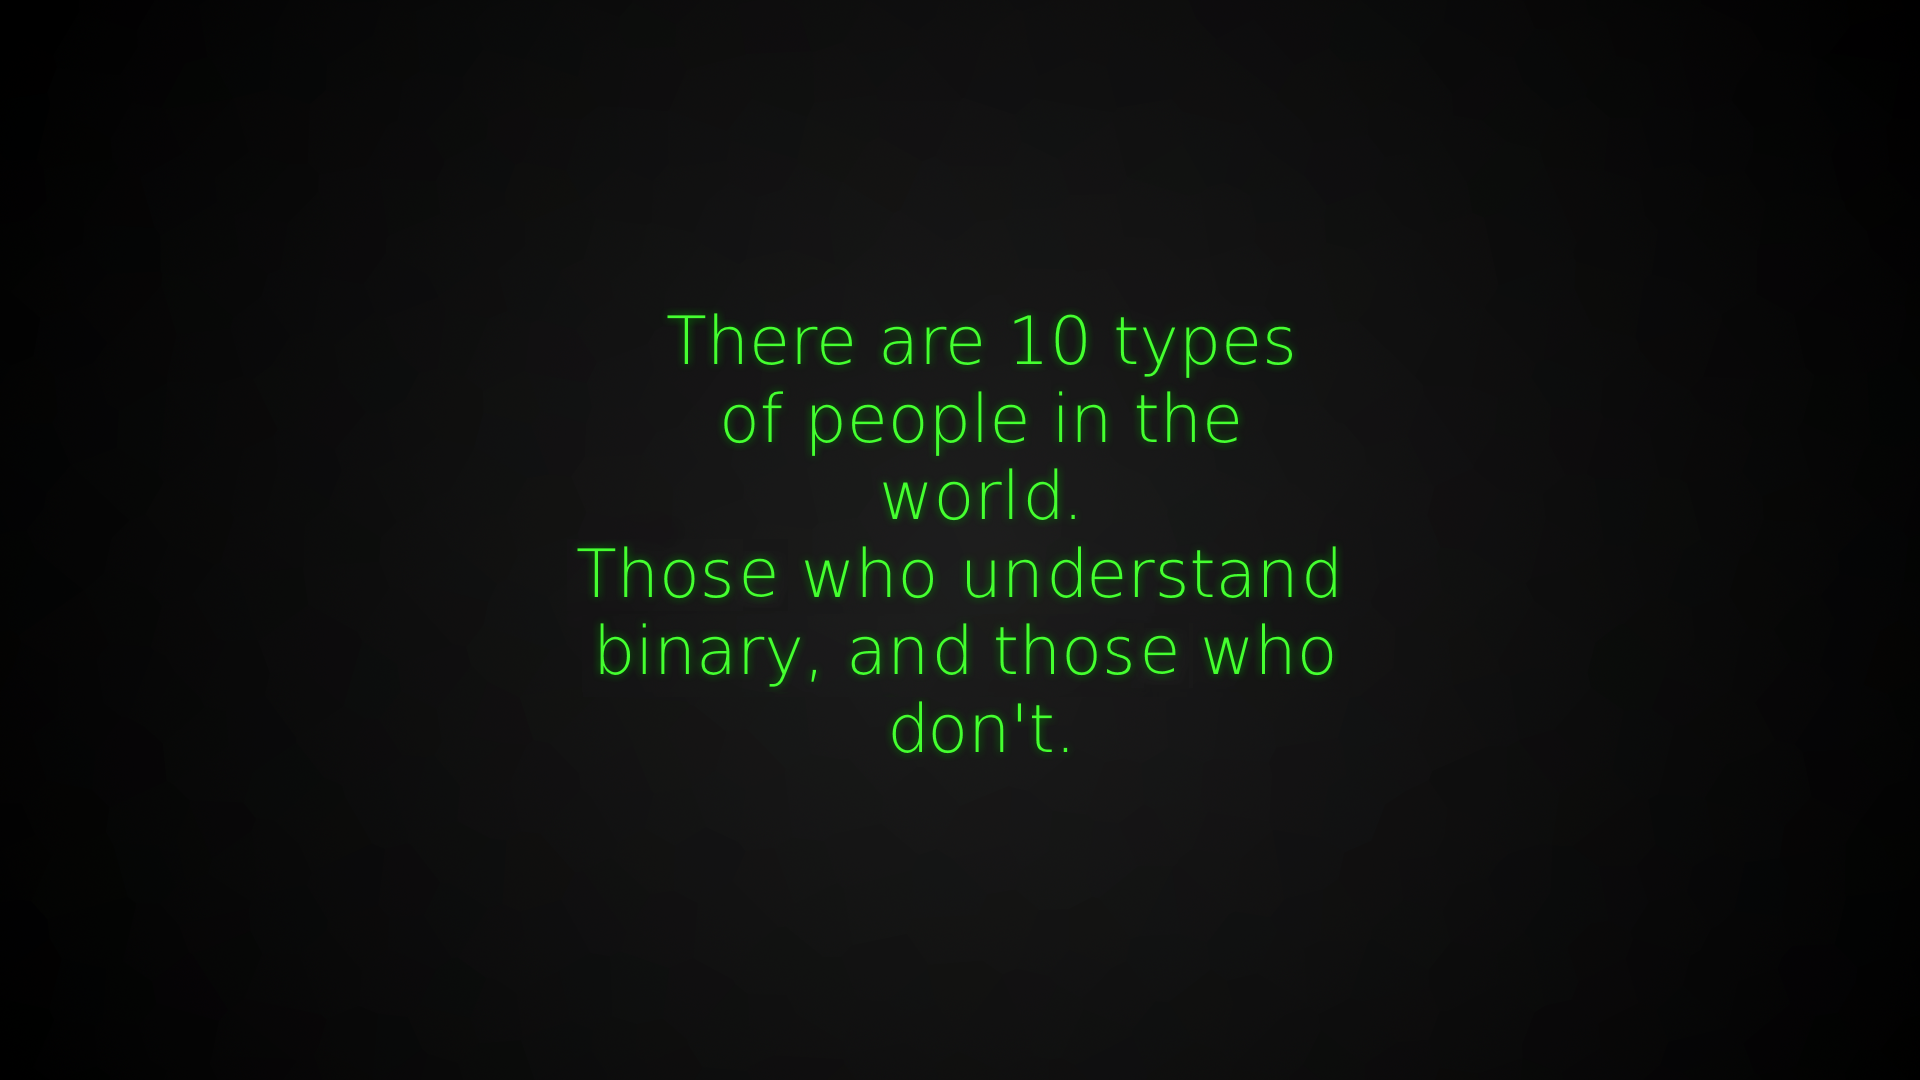
\includegraphics[width=0.85\textwidth]{images/binary_joke}
	% https://imgur.com/gallery/QkR1X
	\caption{A popular joke among nerds.}
	\label{fig:binary_joke}
\end{figure}

\section{Decimal to Binary Conversion}
Now, let’s look at the opposite conversion, converting decimal numbers to
binary. This will use successive division and subtraction as opposed to
addition and multiplication. We will divide by two. Then, if the
remainder is non-zero, we’ll keep a 1 at the current position. Otherwise, we'll write down a 0. We’ll
continue until we can no longer divide by two. We will use a table for this, where the first column is the number at the current step in the process; the second column is that number divided by 2 (excluding the remainder); and the third column is a 1 if there was a remainder and 0 otherwise. Here's the process for writing the binary representation of 33: 

\begin{center}
\begin{tabular}{|c|c|c|}
\hline
\textbf{Initial Value} & \textbf{Divided by 2} & \textbf{Remainder} \\
\hline
  4 &   2 & 0 \\
  2 &   1 & 0 \\
  1 &   0 & 1 \\
\hline
\end{tabular}
\end{center}

$$4 = 100_2$$

To walk through the process, 4 divided by 2 is 2. There is no remainder, so we put 2 in the second column and a 0 in the third column. We then moved 2 down to the first column in the next row. We divided 2 by 2 and got 1, which has no remainder so we wrote 0 in the last column. We brought down the 1, divided by 2 and got 0.5 (i.e. ``0 with a remainder of one"). So we wrote 0 in the second column, but for the remainder we put 1 in the third column. We then simply wrote down the string of numbers in the third column starting at the bottom and going up. 

Let's walk through one more example together: what is the binary representation of 13? 

\begin{center}
\begin{tabular}{|c|c|c|}
\hline
\textbf{Initial Value} & \textbf{Divided by 2} & \textbf{Remainder} \\
\hline
  13 &   6 & 1 \\
  6 &   3 & 0 \\
  3 &   1 & 1 \\
  1 &   0 & 1 \\
\hline
\end{tabular}
\end{center}

$$13 = 1101_2$$

To walk through the process, 13 divided by 2 is 6.5 (i.e. ``6 with a remainder of one"). There is a remainder, so we put 6 in the second column and a 1 in the third column. We then moved 6 down to the first column in the next row. We divided 6 by 2 and got 3, which has no remainder so we wrote 0 in the last column. We brought down the 3, divided by 2, and got 1.5 (i.e. ``1 with a remainder of one"). So we wrote a 1 in the second column and 1 in the third column. We brought down the 1, divided by 2 and got 0.5 (i.e. ``0 with a remainder of one"). So we wrote 0 in the second column and 1 in the third column. We then simply wrote down the string of numbers in the third column starting at the bottom and going up. 

It is also possible to convert decimal numbers that have a fractional part using this same method, but it can get challenging so we won't do it in this course. 

\begin{example}
The numbers below are represented in base 10, or decimal. Write down their base 2, or binary, representation. 
\begin{enumerate}
\item $1$
\item $2$
\item $5$
\item $10$
\item $20$
\item 
\end{enumerate}
\noindent \emph{Answer}:
\begin{enumerate}
\item $1_{2}$
\item $10_{2}$
\item $101_{2}$
\item $1010_{2}$
\item $10100_{2}$
\end{enumerate}
\end{example}

\section{Binary Addition}
Just as we perform addition with decimal numbers, we can perform addition with
binary numbers. The process is exactly the same, except we work with bits (1s and 0s) instead of
digits (0 through 9). Let’s start by looking at addition and multiplication in decimal.

\begin{align*}
15&\\
\underline{+\hspace{1mm}6}&\\
21&\\
\end{align*}

To get there, we looked at the rightmost numbers and added them to get 11 (i.e. ``10 remainder 1"). So we wrote down the remainder of 1 below the black line, and put a one on top of the line to the left. We then added 1 to 1 on the next line to get 2. Here's another example: 

\begin{align*}
26&\\
\underline{+\hspace{1mm}17}&\\
30&\\
\end{align*}

Here we looked to the rightmost numbers, adding 6 to 7 to get 13 (i.e. ``10 remainder 3"). We wrote down the remainder of 3 below the line and carried a 1 (for the 10) to the top of the next column. We then added 1, 2, and 3 in that column to get 6. Let's try one more:

\begin{align*}
55&\\
\underline{+\hspace{1mm}60}&\\
115&\\
\end{align*}

We went to the rightmost numbers and added them: 5 and 0 give 5 (i.e. ``0 remainder 5"). So we wrote down the remainder of 5 below the line and didn't need to carry anything. We moved left and added 5 to 6 to give 11 (i.e. ``10 remainder 1"). So we wrote down a 1 and moved a 1 to the next column (which was empty). We then simply brought down the 1. 

The process is exactly the same for binary numbers! Instead of have 10 with remainders, though, we will think about 2 with remainders. Let's jump straight into an example to clarify this, where we'll add $111_{2}$ (7 in decimal representation) to $11_{2}$ (3 in decimal representation). If all goes well, we should get $1010_{2}$, since that is 10 in decimal representation. 

\begin{align*}
111_{2}&\\
\underline{+\hspace{1mm}11_{2}}&\\
1010_2&\\
\end{align*}

Here we looked at the rightmost column and added 1 and 1 together to get 2 (i.e. ``2 remainder 0"). We wrote down the remainder of 0 below the line and carried a 1 (for the 2) to the top of the next column. We then had to add 1, 1, and 1, which gives us 3 (i.e. ``2 remainder 1"). So we wrote a 1 below the line (for the remainder of 1) and carried a 1 (for the 2). Finally, we added 1, 1, and 0 to get 2 (i.e. ``2 remainder 0"). So we wrote down 0 below the line and carried a 1 (for the 2). We then simply brought down the 1. 

Let's look at one more example together: 

\begin{align*}
111_{2}&\\
\underline{+\hspace{1mm}111_{2}}&\\
1110_2&\\
\end{align*}

We start on the right and add 1 and 1 to get 2 (i.e. ``2 remainder 0"). So we write 0 below the line and carry a 1. We then add 1, 1, and 1 to get 3 (i.e. ``2 remainder 1"). So we write down a 1 and carry a 1. We then add 1, 1, and 1 to get 3 (i.e. ``2 remainder 1"). We wrote down a 1 and carried a 1 (for the 2). We then simply brought down the 1. 

\begin{example}
Add the following binary numbers. Give your answer in binary representation. 
\begin{enumerate}
\item $1_2+1_2$
\item $11_2+1_2$
\item $101_2+111_2$
\item $1110_2+1_2$
\end{enumerate}
\noindent \emph{Answer}:
\begin{enumerate}
\item $10_2$
\item $100_2$
\item $1100_2$
\item $1111_{2}$
\end{enumerate}
\end{example}

Subtraction, multiplication, and division of binary numbers also involves the same process as decimal numbers. However, we won't go over these in this course. 

%\noindent%
%\begin{minipage}{.5\linewidth}
%\begin{align*}
%10110101_2&\\
%\underline{+\hspace{1mm}1010110_2}&\\
%100001011_2&\\
%\end{align*}
%\end{minipage}%
%\begin{minipage}{.5\linewidth}
%\begin{align*}
%110101_2&\\
%\underline{\times\hspace{3mm}1101_2}&\\
%110101_2&\\
%11010100_2&\\
%\underline{+\hspace{1mm}110101000_2}&\\
%1010110001_2&\\
%\end{align*}
%\end{minipage}

%Here we see how to add the binary representations of 181 and 86 and get 267 as the
%result. We also see how to do long form multiplication of 53 and 13 to get 689. You’ll
%notice this is exactly the same as for decimal numbers but we force ourselves to only
%work with bits, carrying the one to the next place when necessary. Both subtraction
%and division work similarly.

\section{Bit-wise Operators}

Now we’ll turn our attention to three important arithmetic operations on binary numbers:
\textbf{and}, \textbf{or}, and \textbf{exclusive or} (\textbf{xor}). These are
called ``bit-wise operations" as they apply to each bit place, one at a time. We therefore can simply line up two binary numbers, padding with 0s on the left of the shorter binary number if they are different lengths (which doesn't change its value). We'll see an example of the process later, but first let's understand what the operators do to an individual set of 2 bits.  

When looking at two binary numbers, \textbf{and} is an operation that gives 1 if both bits are 1, and 0 otherwise (i.e. answers ``the first \textbf{and} second bit are both 1?"). The \textbf{or} is an operation that gives 1 if either bit (or both bits) is 1 (i.e. answers ``is either/or bit 1?"). Finally, the ``exclusive or", or \textbf{xor}, is an operation that gives 1 if either bit (but \textit{not} both) is 1 (i.e. answers ``is exclusively one of the bits 1?"). The following table lists out the result of each operation on every combination of 0 and 1. 

\begin{center}
\begin{tabular}{|c|c|c|c|c|}
\hline
$a$ & $b$ & $a$ \textbf{and} $b$ & $a$ \textbf{or} $b$ & $a$ \textbf{xor} $b$ \\
\hline
0   &  0  &  0  &  0  &  0  \\ 
0   &  1  &  0  &  1  &  1  \\
1   &  0  &  0  &  1  &  1  \\
1   &  1  &  1  &  1  &  0  \\
\hline
\end{tabular}
\end{center}

Now that we know how to operate on any two bits, we can simply line up any two binary numbers (with left-zero padding as necessary) and use the operator on each set of bits. Here are a few examples: 

To do $111_2\textbf{and}110_2$:
\begin{align*}
111_2 &\\
\underline{\textbf{and}\hspace{2mm}110_2}&\\
110_2 &\\
\end{align*}

In this example, the two numbers are the same length so we don't need to pad any zeros. Starting with the rightmost bits, we have $1\mathbf{and}0$ which is $0$. Moving to the left, we have $1\mathbf{and}1$, which is 1. Moving to the left again, we have $1\mathbf{and}1$, which is 1

Now let's do $101_2\mathbf{or}11_2$:
\begin{align*}
101_2 &\\
\underline{\mathbf{or}\hspace{4mm}011_2}&\\
111_2&\\
\end{align*}

In this case, since $11_2$ is shorter than $101_2$, we needed to pad the 11 with a single 0 on the left so it was also three bits long. We then did bit-wise comparison: from right to left we saw $1\mathbf{or}1$ is $1$, $0\mathbf{or}1$ is $1$, and $1\mathbf{or}0$ is $1$. 

Now let's do $111_2\mathbf{xor}1_2$:
\begin{align*}
101_2 &\\
\underline{\mathbf{xor}\hspace{4mm}001_2}&\\
100_2 &\\
\end{align*}

Since $111_2$ has three bits and $1_2$ only one, we pad two zeros on $1_2$ to get $001_2$. We then go from right to left with the \textbf{xor} operation, getting $1\textbf{xor}1=0$, $0\textbf{xor}0=0$, and $1\textbf{xor}0=1$.

Finally, try $111_2\mathbf{and}1_2$:
\begin{align*}
101_2 &\\
\underline{\mathbf{and}\hspace{4mm}001_2}&\\
1_2 &\\
\end{align*}

As in the previous example, since $111_2$ has three bits and $1_2$ only one, we pad two zeros on $1_2$ to get $001_2$. We go from right to left with \textbf{and}, getting $1\textbf{and}1=1$, $0\textbf{and}0=0$, and $1\textbf{and}0=0$. So our results is $001_2$. However, since left-padded 0s don't change the number this is the same as $1_2$. 

\begin{example}
Perform the following binary operations. Give your answer in binary representation. 
\begin{enumerate}
\item $1_2 \textbf{xor}1000_2$
\item $10_2 \textbf{or} 10_2$
\item $1111_2 \textbf{and} 1011_2$
\item $1111_2 \textbf{or} 1011_2$
\end{enumerate}
\noindent \emph{Answer}:
\begin{enumerate}
\item $1001_2$
\item $10_2$
\item $1011_2$
\item $1111_{2}$
\end{enumerate}
\end{example}

\exercisesection

\begin{exercise}
Write the radix decomposition for each of these decimal numbers. For example, 1.2's radix expansion is $1\times10^0 + 2\times10^{-1}$
\begin{enumerate}
\item 193 
\item 5.2
\item 1,984
\item 7.39
\end{enumerate}
\end{exercise}

\begin{exercise}
Write out the radix decomposition for each of these binary numbers. For example, $1.1_2$'s radix expansion is $1\times2^0 + 1\times2^{-1}$. 
\begin{enumerate}
\item $11_2$
\item $10.1_2$
\item $1.01_2$
\item $111_2$
\end{enumerate}
\end{exercise}

\begin{exercise}
Write out the decimal form of the following binary numbers. For example, $1.1_2$'s in decimal form is $1.5$. These are the same numbers as in the previous exercise, so feel free to use the radix decompositions you already wrote down. 
\begin{enumerate}
\item $11_2$
\item $10.1_2$
\item $1.01_2$
\item $111_2$
\end{enumerate}
\end{exercise}

\begin{exercise}
Write out the binary form of the following decimal numbers. 
\begin{enumerate}
\item 6
\item 15
\item 22
\item 80
\end{enumerate}
\end{exercise}

\begin{exercise}
Add the following binary numbers. Write the answer in binary form. 
\begin{enumerate}
\item $1_2 + 0_2$
\item $111_2+1_2$
\item $111_2+111_2$
\item $101_2+100_2$
\end{enumerate}
\end{exercise}

\begin{exercise}
Evaluate the following bit-wise operations. Write the answer in binary form. 
\begin{enumerate}
\item $1_2 \mathbf{and} 0_2$
\item $111_2 \mathbf{or} 1_2$
\item $111_2 \mathbf{xor} 111_2$
\item $101_2 \mathbf{and} 100_2$
\end{enumerate}
\end{exercise}
    
    \chapter{Fantastic Errors and Where to Find Them (Debugging)}

\section{Introduction}

In the previous lab sessions you wrote some code. Most probably, your code didn't work at first. What you had is called a bug, and it is the nemesis of programmers since times untold. The term has been used in as early as $1878$\footnote{https://en.wikipedia.org/wiki/Debugging}. Back in the days computers were room-sized heavy machines, some bugs were literally bugs stuck in the machinery. Nowadays, bugs mostly live in our code.

\begin{marginfigure}
\centering
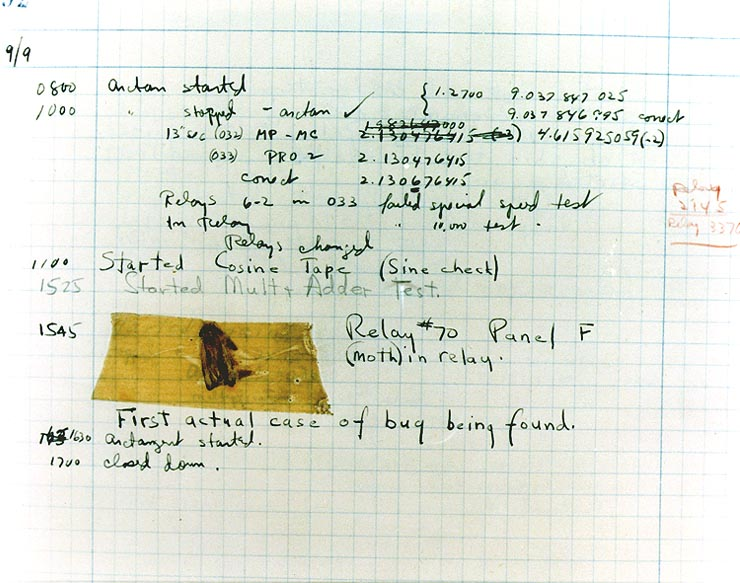
\includegraphics[width=.9\linewidth]{images/bug.jpg}
\caption{An early documented bug, found in the Mark II computer, 1947. Courtesy of the Naval Surface Warfare Center, Dahlgren, VA., 1988. / Public domain}
\end{marginfigure}

In this lesson we'll learn about bugs and how to fight them. 

\begin{definition}
\emph{debugging} is the process of identifying and removing errors from computer hardware or software.
\end{definition}

Debugging is like detective work, and it is a skill that can be trained, just like writing code. But before we start debugging, we first need to learn the basic terminology, and the way DrJava will report bugs and other problems to us. Let's start with a classification of problems in a program:

\begin{definition}
\leavevmode\newline
\begin{itemize}
    \item a \emph{compilation error} is an problem encountered during the compilation process, before running the code. A code with compilation errors cannot be run.
    \item a \emph{runtime error} is encountered while the code is running, after it has been successfuly compiled. It typically represents a serious problem that should stop the code once encountered.
    \item an \emph{exception} is also encountered while the code is running. It typically represents a problem that an application can try to recover from and keep running.
    \item a \emph{bug} is a flaw in a program that causes it to behave in unintended ways. This can include the program encountering errors or exceptions, but can also lead to a program that runs without either of these errors but in an incorrect way, in which case we will call it a \emph{silent bug}.
\end{itemize}
\end{definition}

The exact distinction between errors and exceptions is soft, and varies between languages. The Java language also distinguishes between two types of exceptions, checked and unchecked, but we won't go over the distinction here.

\section{Compilation Errors}

Let's look at the following example:

\begin{example}
What's wrong with the following code?

\begin{code}
public class Snippet{
    public static void main(String []args){
        int x = 5.5;
    }
}
\end{code}
\end{example}

This code will result in a compilation error. Let's look at the message DrJava will display when trying to compile this code, in figure~\ref{fig:type_mismatch}.

\begin{figure}[h!]
\centering
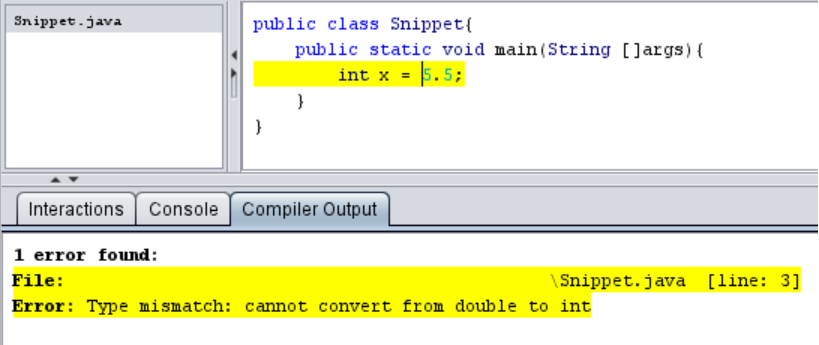
\includegraphics[scale=0.8]{images/incompatible_types.PNG}
\caption{An incompatible type error.}
\label{fig:type_mismatch}
\end{figure}

The line the compiler got stuck at is highlighted in yellow, helping us focus on the likely cause of the error. In the "Compiler Output" window, we see three lines that give us information on our problem:

\begin{enumerate}
    \item "1 error found:"
    Sometimes the compiler is able to put aside an error and keep trying to compile the rest of the code, so we could see as much errors we made as possible. The number of errors the compiler was manage to find is listed here, in our case just one.
    \item "File: ...\\Snippet.java [line: 3]" 
    The first part of the line is the path of the file where the error was found (some part omitted). If our code spanned multiple files, this would help us find the right one to focus on.
    The second part of the line tells us the line number where the error was found. If our code is long this would help us scroll to the relevant part.
    \item "Error: Type mismatch: cannot convert from double to int".
    This part tells us what kind of error was found on this line. In this case, it tells us that the error was a "type mismatch" -- this means that we were trying to assign some value to a variable of another value, in a way that does not make sense. The rest of the line explains why this assignment did not make sense -- we were assigning a double value, $5.5$, to an $int$ variable, but a double value can't be converted to an $int$ in a safe manner.
\end{enumerate}

By focusing our attention on the location of the error, and telling us what kind of error it was, the compiler helps us identify and fix it quickly. Sometimes, however, errors are trickier to find, as in this example:

\begin{example}
What's wrong with the following code?

\begin{code}
public class Snippet{
    public static void main(String []args){
        int x = 5.5;
    
}
\end{code}
\end{example}

This code has the same error as the previous one, but there's another problem with it - the $\}$ sign that was supposed to end the $main$ block is missing. Let's look at the compiler output for this code, in figure~\ref{fig:syntax_error}:

\begin{figure}[h!]
\centering
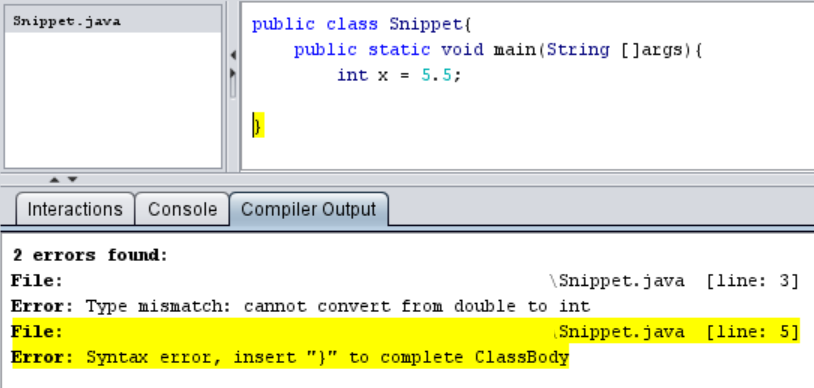
\includegraphics[scale=0.8]{images/syntax_error.PNG}
\caption{A new syntax error joins the previous error.}
\label{fig:syntax_error}
\end{figure}

First, notice that the compiler was able to found both errors. If we click on the two lines corresponding to each error, DrJava will highlight the relevant row in our code. 

The new error we encountered is called a syntax error. Like any spoken and programming language, Java has a syntax that's required to build meaningful commands. This includes ending statements with a semicolon $;$, closing any open $"$, $\{$, $($ and $[$ and more (we'll see more examples in the assignment). In our case, the block of the $main$ method has to start with a $\{$ and end with a $\}$. If not, the compiler won't be able to figure out where the $main$ method ends.

This is exactly what is happening here -- the compiler can't know what the $\}$ is closing here, it just finished scanning the entire code and realized it is still missing one $\}$. In more complicated code, the compiler might not be able to point us close enough to the problematic line, so with syntax errors we need to be extra careful going over our code.

\section{Runtime Errors and Exceptions}

Problems that happen during a program's run are generally more difficult than compilation problems. That is because often these problems \emph{might} happen, but don't \emph{necessarily} happen. Moreover, a program might reach a certain line of code multiple times during its execution. This makes it harder to figure out when our program failed, and so why it failed.

Let's take a look at several examples of runtime errors and exceptions, and the information that Java (through DrJava) gives us to help investigate them.

\begin{example}
Look at the following program's code. Does it do what it claims to do? Can it run into a problem?

\begin{code}
import java.util.Scanner;

public class Snippet{
    public static void main(String []args){
      // Takes a number as input from the user, and prints the number back with a message.
      Scanner input = new Scanner(System.in);
      String token = input.next();
      int num = Integer.parseInt(token);
      System.out.println("The number you chose is: " + num);
    }
}
\end{code}
\end{example}

This code compiles without a problem, and seems to do what it claims -- it scans an input from the user, treats it as a number, and prints it back with a message. Now, let's look at two possible executions of the program, shown in figure~\ref{fig:number_format_error}

\begin{figure}[h!]
\centering
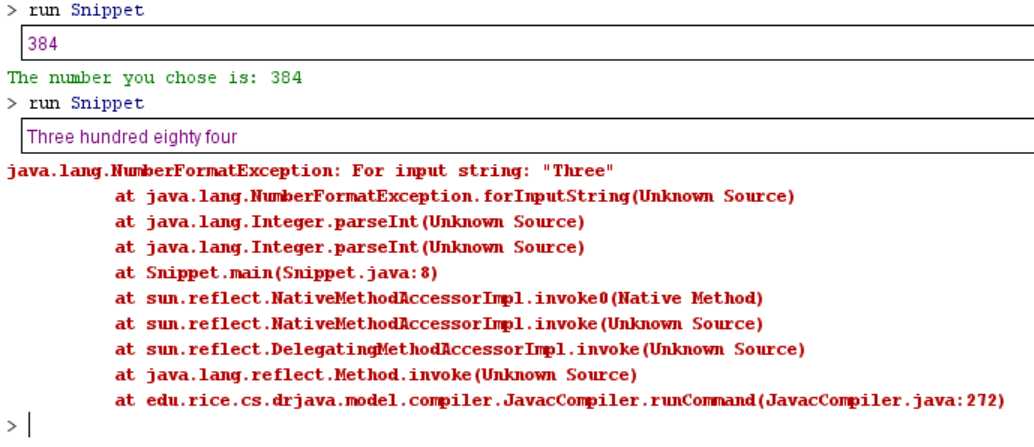
\includegraphics[scale=0.7]{images/number_format_exception.PNG}
\caption{Two executions of the program, one causing an exception.}
\label{fig:number_format_error}
\end{figure}

The first time the program was run, the user wrote $384$ as an input, and the program ran fine. The second time, however, the user wrote the number using words. Integer.parseInt wasn't able to parse the token it got, "Three", and \emph{threw} an exception. Our program didn't recover from the exception, and instead terminated.

The first red line below our execution prompt lists the type of exception and its details. The exception was NumberFormatException (ignore the prefix "java.lang."). The rest of the line details that the problem was encountered given the input "Three".

The red lines that follow are called the \emph{stack trace}, and they are very important for understanding when and where our code failed. Before we read them, let's do a little imagination exercise. Think of running of a program as a little turtle traveling code lines and executing them (this is slightly inaccurate, but close enough!). Figure ~\ref{fig:turtles} shows the journey of the turtle throughout the code in the last example, before it crashes with the exception we saw. 

\begin{figure}[h!]
\begin{subfigure}{1\textwidth}
  \centering
  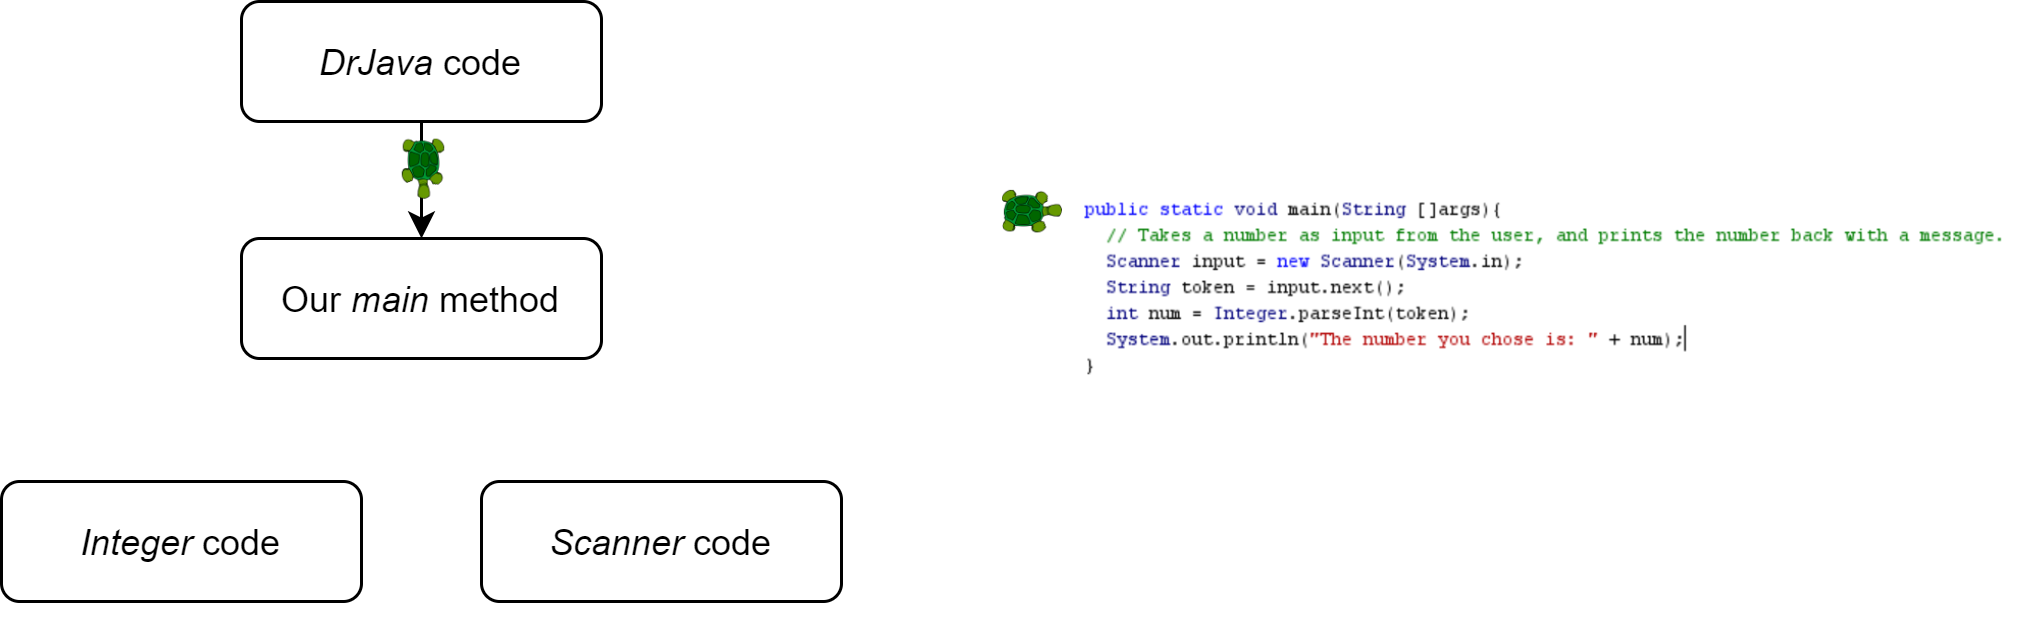
\includegraphics[width=1\textwidth]{images/code_turtle_1.png}
  \caption{}
  \label{fig:sturtle1}
\end{subfigure}%

\begin{subfigure}{1\textwidth}
  \centering
  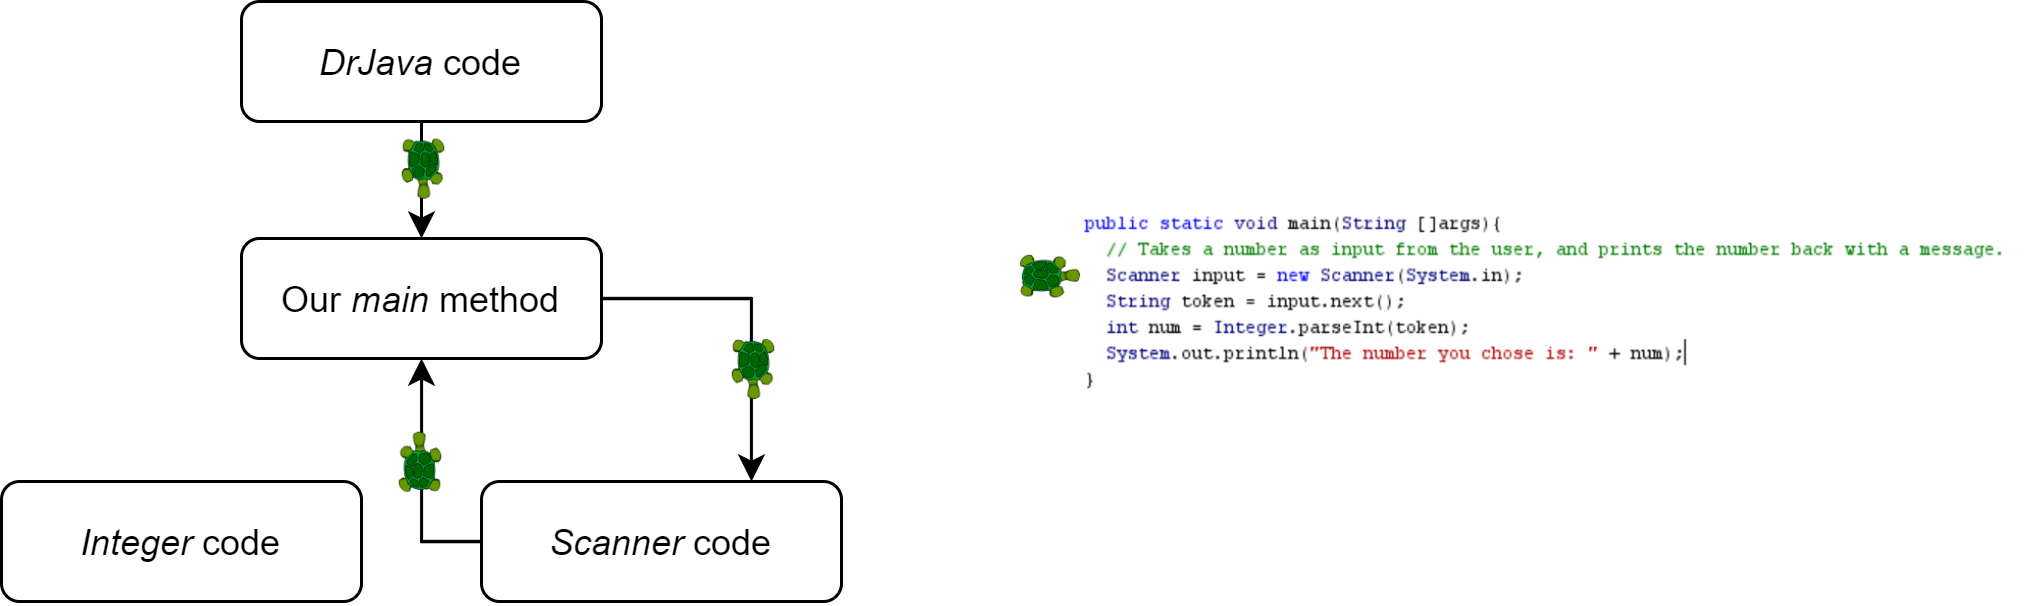
\includegraphics[width=1\textwidth]{images/code_turtle_2.png}
  \caption{}
  \label{fig:sturtle2}
\end{subfigure}%

\begin{subfigure}{1.\textwidth}
  \centering
  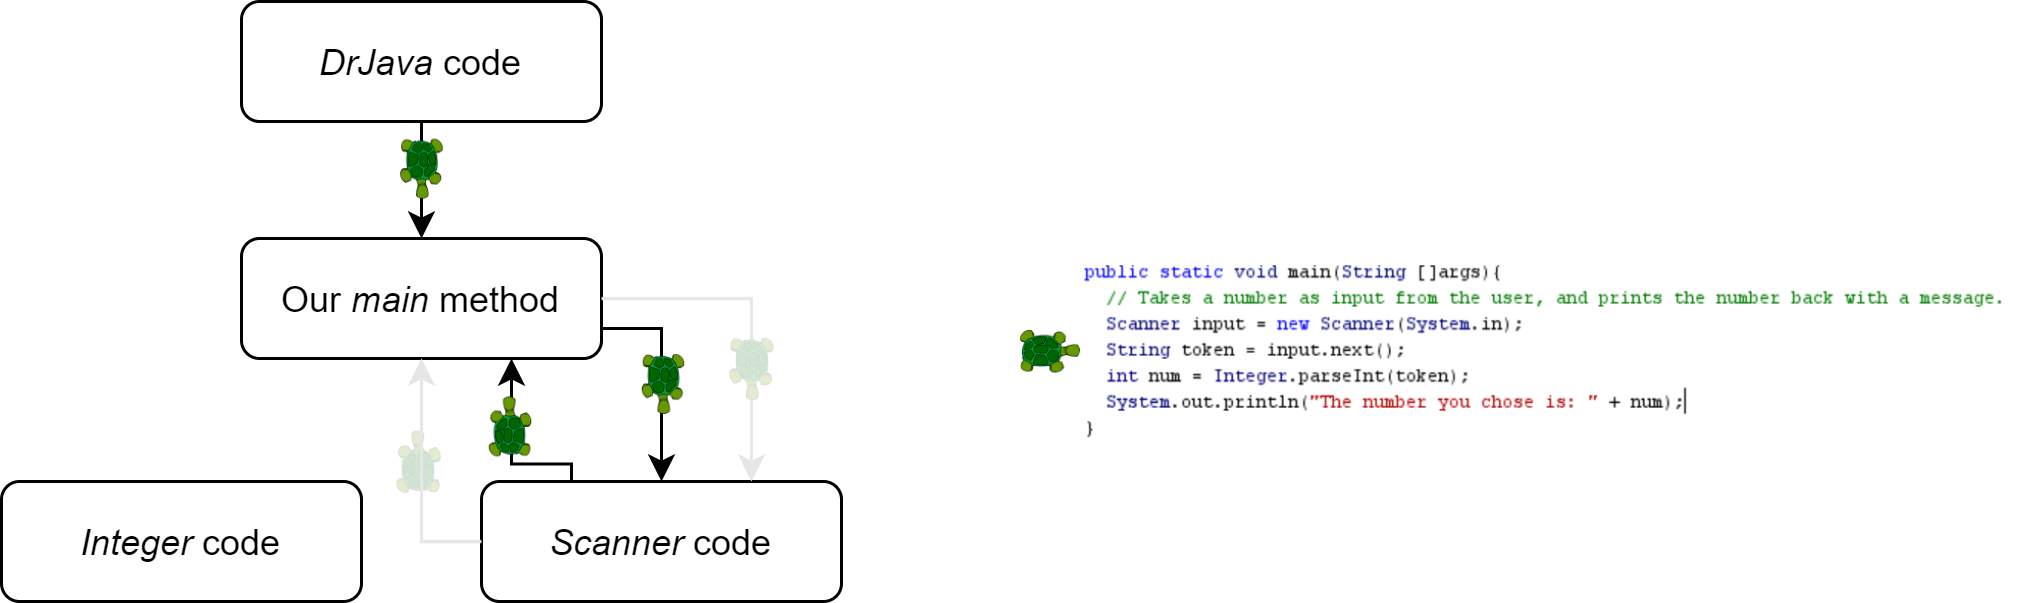
\includegraphics[width=1\textwidth]{images/code_turtle_3.png}
  \caption{}
  \label{fig:sturtle3}
\end{subfigure}%

\begin{subfigure}{1.\textwidth}
  \centering
  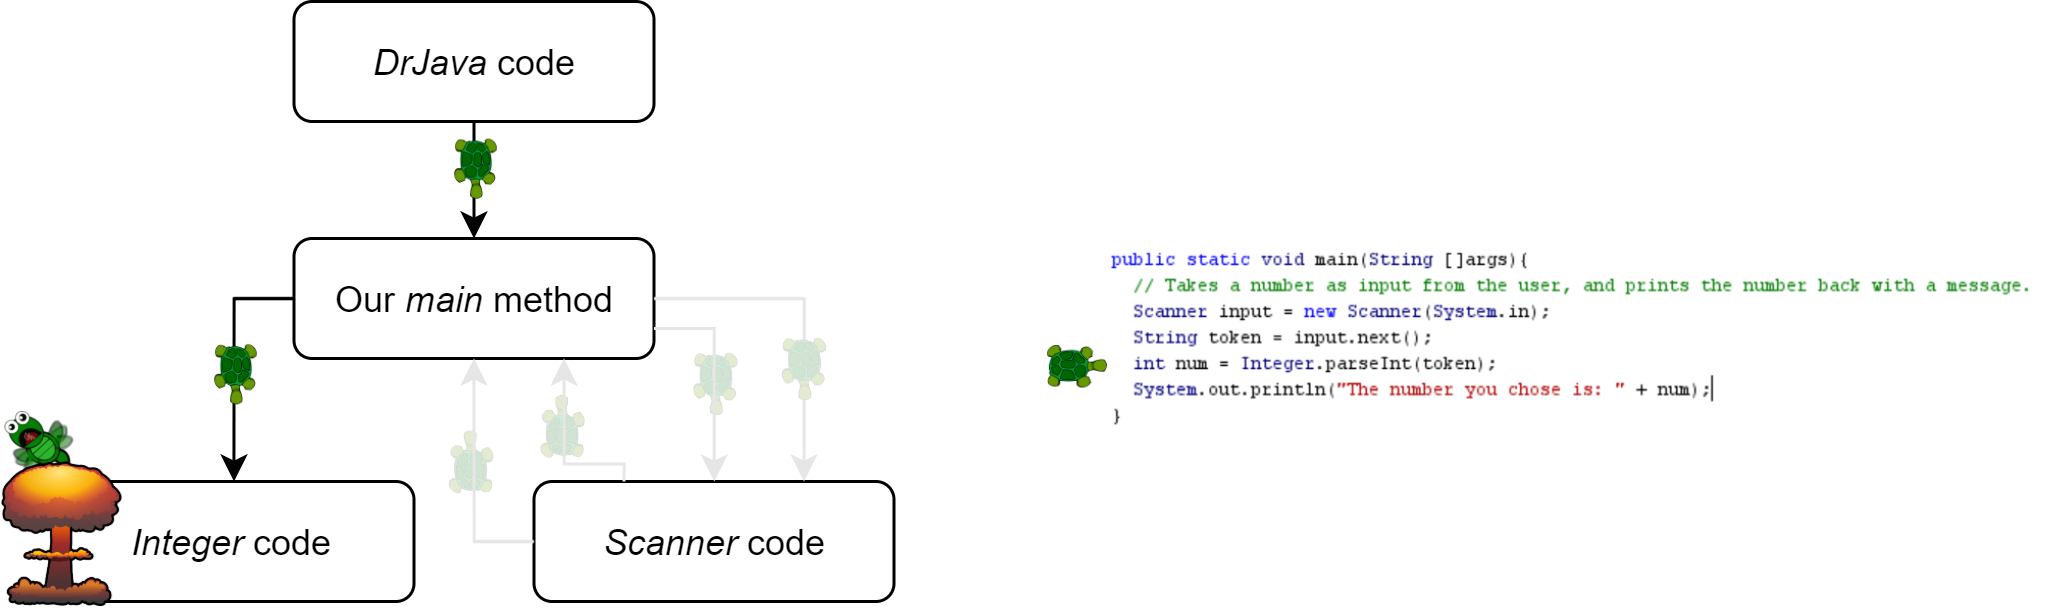
\includegraphics[width=1\textwidth]{images/code_turtle_4.png}
  \caption{}
  \label{fig:sturtle4}
\end{subfigure}%

\caption{The execution of our code. \ref{fig:sturtle1}: Execution enters our \textit{main} method. \ref{fig:sturtle2}: Execution enters the code of \textit{Scanner} to execute "new Scanner(System.in)". After completion, it returns to our \textit{main} method. \ref{fig:sturtle3}: Execution enters \textit{Scanner} code again due to the "input.next()" call, and returns when done. \ref{fig:sturtle4}: Execution enters the code of \textit{Integer} to execute "Integer.parseInt(token)". While there, it encounters an Exception.}
\label{fig:turtles}
\end{figure}



In \ref{fig:sturtle1}, out turtle heads off from whatever code DrJava executes when we click "Run" and enters our code. It starts traversing the code line by line, executing whatever statement is written in each line. In \ref{fig:sturtle2}, the turtle reaches \emph{new Scanner(System.in)} which it needs to execute. This leads the turtle to the code defining \emph{Scanner}, which we're unaware of. The turtle executes whatever lines are written there (there may be many), and then finishes and returns to our code. The turtle continues its journey in \ref{fig:sturtle3} and \ref{fig:sturtle4}, until it reaches the line 

\begin{code}
int num = Integer.parseInt(token);
\end{code}


% In \ref{fig:sturtle3} the turtle goes on to execute the next line. This includes running \emph{input.next()}, and assigning it to the variable token. Since \emph{input} is a \emph{Scanner} variable, the code that's being run when calling \emph{input.next()} is defined in the Scanner code files, and so the turtle makes another trip there and back.

% In \ref{fig:sturtle4} our turtle reaches the offending line, \emph{int num = Integer.parseInt(token)}. To execute it, the turtle heads over to the \emph{Integer} code. Remember that the user gave a wrong input in this execution, and so somewhere in that code our turtle will encounter an exception and stop whatever it was doing.

The stack trace is meant to trace the places our turtle visited on the way to an exception. It ignores any trips the turtle completed successfully, like the two trips to the \emph{Scanner} code. In our case, it should specify the places visited in the DrJava code, our \emph{main} method and the \emph{Integer} code.

The stack trace should be read starting with the bottom line. The bottom five lines all belong to the DrJava code, and in general we can ignore whatever comes below our \emph{main} method, in this case \emph{Snippet.main(Snippet.java:8}. That line tells us that the turtle encountered the exception after visiting line 8 of the \emph{main} method we wrote on the \emph{Snippet} class. The visit to the \emph{Integer} code, and the places the turtle visited there, are traced in the lines above. 

When we write code for bigger projects, our code can become very long, and be separated to many functions and written over many files. An execution can also pass through the same line of code more than once, arriving from different places each time. The stack trace can help us pinpoint the place our code failed at, and figure out how it got there.

% Notice that sometimes the compiler can catch problems that only might happen during compilation. In these cases, it will notify use during compile time.
% public class Snippet{
%     public static void main(String []args){
%       Scanner input = new Scanner(System.in);
%       String userNumber = input.next();
%       int weight = Integer.parseInt(userNumber);
      
%       String response;
%       if(weight > 25){
%         response = "good";
%       }
%       System.out.println(response);
%     }
% }



% \section{Throwing and Catching Exceptions}

% You can also throw errors, just mention.

\section{Debugging Tactics}

Now that we've goetten familiar with errors, we can talk about different ways by which we can investigate our errors and solve them. If our program has compilation errors, it was never run, and so the error message is all we have to investigate the error with.

Runtime errors and exceptions, however, happen at some point during the program's execution, and they don't necessarily happen every time we run it. Even worse, silent bugs also happen while the program executes, but since those are just the gap between our intentions and the code we wrote, the Java language can't stop and tell us about them when they're encountered.

Before we go on to cover some specific methods for debugging, let's outline the general approach we can take to detect, isolate and fix errors:

\begin{enumerate}
\item Reproduce the error: Find a condition that causes the error to happen. Ideally, understand exactly what conditions causes that.
\item Isolate the error: Find the parts of your code related to the error. If possible, temporarily disable other parts to simplify the program.
\item Identify the cause: Go over your code carefully, and find out how the code behaves differently than you expected it to.
\item Implement and test fix: Re-write your code to take care of the existing problem, then test your code to see that it's working properly.
\end{enumerate}

Different debugging tools and methods relate to the different steps outlined above. For example, unit tests and test driven development (that we'll cover later) help with reproducing, isolating and testing fixes to errors. A debugger is a tool that helps us track the execution of a program (we'll cover jdb, the Java debugger, later), and a profiler helps track the memory consumption and running time of parts in a program.

Here we will focus on the general approach outlined before, and a basic method for debugging called \emph{logging}:

\begin{definition}
\emph{Logging} is the act of printing information about the state of a program while it runs, either to the screen or to a designated \emph{log file}. 
\end{definition}

Logging is an important technique in situations where we can't observe our code as it runs, such as on software that is being run on a system belonging to our client. The information we logged then helps us investigate our program in retrospect. The simplicity of logging, however, allows us to start using it early on in coding, before we learn to use powerful tools like a debugger. Let's try out tackling an error with logging, using this example:

\begin{example}
Look at the following code, that has a bug. Assume the user can be trusted to input only positive integer numbers. 

\begin{code}
import java.util.Scanner;

public class Snippet{
    public static void main(String []args){
        // Get an integer input from the user. Print the product (multiplication) of all positive integers up to this number.
        // If the user gives the number n, should return 1 * 2 * ... * n
        int userNum = 0;
        int product = 0;
        String token;
        Scanner input = new Scanner(System.in);
        System.out.println("Please input a number:");
        token = input.next();
        userNum = Integer.parseInt(token);
        
        for(int i = 1; i <= userNum; i++){
            product = product * i;
        }
        
        System.out.println("Product: " + product);
    }
}
\end{code}

\end{example}

We still haven't encountered the error ourselves. As a first step in our investigation, after reading the code, we should reproduce the error. Let's run the code and input different legal values to see what the output is, shown in figure~\ref{fig:bug}.

\begin{figure}[h!]
\centering
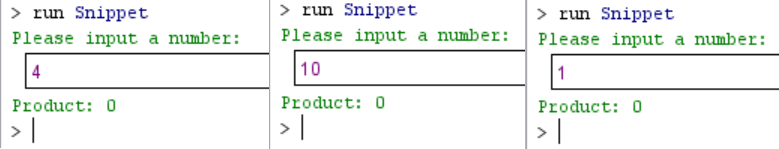
\includegraphics[scale=0.8]{images/bug_outputs.png}
\caption{Multiple executions of our program. The correct outputs corresponding to the inputs $4,10$ and $1$ are $24, 3628800$ and $1$.}
\label{fig:bug}
\end{figure}

It seems like the program incorrectly prints $0$ for every input. Now that we've reproduced the error, we want to isolate it. Our program prints the value of the variable \ic{product}. That variable is supposed to hold the product of the numbers between $1$ and \ic{userNum}. Let's focus on the loop that updates \ic{product}:

\begin{code}
for(int i = 1; i <= userNum; i++){
    product = product * i;
}
\end{code}

It seems to multiply the variable by all numbers up to \ic{userNum}, as needed. We can use logging to track the value of this variable throughout the program's run, like this:

\begin{code}
import java.util.Scanner;

public class Snippet{
    public static void main(String []args){
        // Get an integer input from the user. Print the product (multiplication) of all positive integers up to this number.
        // If the user gave the numebr n, should return 1 * 2 * ... * n
        int userNum = 0;
        int product = 0;
        System.out.println("Value of product after initialization: " + product);
        String token;
        Scanner input = new Scanner(System.in);
        System.out.println("Please input a number:");
        token = input.next();
        userNum = Integer.parseInt(token);
        System.out.println("Value of product after taking user input: " + product);
        
        for(int i = 1; i <= userNum; i++){
            product = product * i;
            System.out.println("Value of product after loop iteration: " + product);
        }
        
        System.out.println("Product: " + product);
    }
}
\end{code}

Running this program with the input $3$ results in the output shown in figure~\ref{fig:logging}. 

\begin{figure}[h!]
\centering
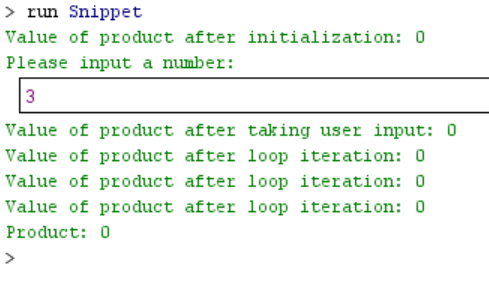
\includegraphics[scale=0.8]{images/logging.PNG}
\caption{Running the program with logging.}
\label{fig:logging}
\end{figure}

We can see that the value of \ic{product} was $0$ throughout the execution of the program. This explains why the value didn't change between iterations of the loop -- multiplying $0$ by any number results in $0$. We thus know that the problem must originate from the initialization of \ic{product}: 

\begin{code}
int product = 0;
\end{code}

Now we know the cause of the problem. Initializing \ic{product} to $0$ made all the multiplications later useless, since the value remained $0$. 

We can now implement a fix to the problem, by initializing \ic{product} with a value that will allow it to change between iterations of the loop. Since we are already supposed to multiply with all the numbers up to \ic{userNum}, we can choose $1$ for the initial value, which is neutral to the multiplication.  After implementing the change, all that's left is to check the new outputs of the program, by running it again with different inputs.

Later in the course, our toolbox for debugging will grow. Logging by printing values, however, can serve us in the meantime to implement the general approach for finding and fixing errors, as we outlined above.


we should figure out \emph{when} that variable 


It's important, then, that we have a way of investigating our code as it runs. One of the common and powerful methods of doing that is called \emph{step debugging}, 

Even worse, silent bugs happen 

and runtime errors and exceptions, we can start by reading the error messages and stack traces. 

% Talk about preventive programming? (tests, coding patterns and design principles)

% Mention rubberducking?

\section{Closing words}

Debugging is an unrewarding process. when you write code, you see the fruits of your labour -- hours of work transform to lines of code, your will made real for the computer. When you debug, you spend your time, sometimes days, just to end up with a code that does what it was supposed to do when you started.

This is not wasted time, however. This is an important counterpart to writing code, and one that every programmer has to go through.

\begin{mdframed}
% "To err is human, to fix your bugs divine. " -- Stackoverflow user Ward Muylaert

% "Human beings are incapable of avoiding errors. You might as well be embarrassed that you have a nose." from https://www.cis.upenn.edu/~matuszek/General/JavaSyntax/errors.html?


“If debugging is the process of removing software bugs, then programming must be the process of putting them in.” ― Edsger W. Dijkstra

\end{mdframed}

Programmers typically spend half of their programming time debugging\footnote{Britton, Tom, et al. "Reversible debugging software." Judge Bus. School, Univ. Cambridge, Cambridge, UK, Tech. Rep (2013).}. With more practice and better debugging habits, you could make that process more efficient. Regardless, reward yourself when you fix a bug -- it might be invisible, but you're making progress.
    
    \chapter{Input and Output}

Let's look at the ``Hello World'' program that we saw earlier:
\begin{code}
class HelloWorld {

    public static void main(String[] args) {
        System.out.println("Hello World!");
    }

}
\end{code}

When you ran this program, it produced the \emph{output} \ic{Hello World!} on a single line.
Using \ic{System.out.println} is one way in which you can have your programs
produce output. In particular, here \ic{System.out} refers to the \emph{output stream}
that, in our case, is where you see output in the ``Interactions'' tab in DrJava.
The \ic{println} part refers to printing (i.e., outputting) the argument
--the String provided between the parentheses--followed by a linebreak (the \ic{ln} part).
As you might imagine, there are ways to produce output in Java, ranging from printing
to \ic{System.out} with and without linebreaks to writing out image files that
plot data. We can also provide \emph{inputs} to a program in order
to affect what is computed and ultimately outputted.

In this chapter, we will be exploring different ways to produce program output
as well as take program inputs.

\section{Output}
The output of a program is what lets the user who runs it
see any results of the work done in the program.
Consider the following program:
\begin{code}
class HelloWorld {

    public static void main(String[] args) {
        String hi = "Hello";
        String earth = "World";
        String result = hi + " " + earth;
    }

}
\end{code}
This program has no output, so although it will compile and run, you won't
be able to tell that it has done anything!
If you added an output statement, then you'd be able to see that
the program does something. We can try using \ic{System.out.println},
which we've seen already.
\begin{code}
class HelloWorld {

    public static void main(String[] args) {
        String hi = "Hello";
        String earth = "World";
        String result = hi + " " + earth;
        System.out.println(result + "!");
    }

}
\end{code}
Now this program will produce the output as seen when we first ran Hello World program:
\begin{code}
> run HelloWorld
Hello World!
>
\end{code}

Let's take a look at some other ways of printing.
Instead of \ic{System.out.println}, we can use \ic{System.out.print}, which
doesn't print the linebreak after the String provided.
If you change \ic{System.out.println} to \ic{System.out.print} above, and hit
``Run'' in DrJava, you'll see something like this:
\begin{code}
> run HelloWorld
Hello World!>
\end{code}
The \ic{>} that indicates that you can type input into the ``Interactions''
tab is now on the same line as \ic{Hello World!} because the linebreak
wasn't output.

\ic{System.out.println} actually does not require a String to be provided,
so we can actually get the linebreak back by adding a
\ic{System.out.println} statement without the String provided:
\begin{code}
class HelloWorld {

    public static void main(String[] args) {
        String hi = "Hello";
        String earth = "World";
        String result = hi + " " + earth;
        System.out.print(result + "!");
        System.out.println();
    }

}
\end{code}
We now have output that looks like this again:
\begin{code}
> run HelloWorld
Hello World!
>
\end{code}

An alternative is to use the \emph{newline} character \ic{\textbackslash n} that represents a
linebreak:
\begin{code}
class HelloWorld {

    public static void main(String[] args) {
        String hi = "Hello";
        String earth = "World";
        String result = hi + " " + earth;
        System.out.print(result + "!\n");
    }

}
\end{code}

We can provide non-String arguments to \ic{System.out.print} and \ic{System.out.println} as well:
\begin{code}
class HelloWorld {

    public static void main(String[] args) {
        String hi = "Hello";
        String earth = "World";
        String result = hi + " " + earth;
        System.out.print(result + "!");
        System.out.println();
        System.out.println(1);
        System.out.println(10/3.0);
    }

}
\end{code}
Try compiling and running the program above.
Note that \ic{System.out.println(10/3.0);} ends up printing
\ic{3.3333333333333335}, with 16 digits after the decimal point.

We can specify how many digits after the decimal point as well
as specifying a lot of other interesting formatting options
using \ic{System.out.printf} (the \ic{f} here refers to formatting).

When using \ic{System.out.printf}, we provide several arguments
in between the parentheses, with the arguments being separated by
commas.
For example, we can replace \ic{System.out.println(10/3.0)} above
with \ic{System.out.printf("\%f\textbackslash n", 10/3.0)}.
The first argument \ic{"\%f\textbackslash n"} is a String that describes the format of the output.
In this case, \ic{\%f} refers to a floating-point number (i.g. a \ic{float} or \ic{double}),
and by default will print 6 places after the decimal point.
The \ic{\textbackslash n} part is the newline character.
Because we specified \ic{\%f} in the formatting String, we must also provide
a floating point number to replace the \ic{\%f} in the output. Here,
we have provided \ic{10/3.0}.
If we perform this replacement, the output looks as follows:
\begin{code}
> run HelloWorld
Hello World!
1
3.333333
> 
\end{code}

We can specify only 3 decimal places by changing \ic{\%f} to \ic{\%.3f}.
Note that the number is \emph{rounded}, not truncated, so if we have a value like
3.3335 and format it with \ic{\%.3f}, it will be printed out as \ic{3.334}.
The following table provides some common format specifiers (we have already seen
\ic{\%f}):

\begin{tabular}{|l|l|}
\hline
Format Specifier & Effect\\
\hline
\%s,\%S & Formats String\\
\%f & Formats floating point (precision provided between \% and f)\\
\%d & Formats integer\\
\%c & Formats character\\
\%b, \%B & Formats Boolean\\
\hline
\end{tabular}

Using this table, we can actually get the same input that we've been getting
with only one print statement:
\begin{code}
class HelloWorld {

    public static void main(String[] args) {
        String hi = "Hello";
        String earth = "World";
        String result = hi + " " + earth;
        System.out.printf("%s!\n%d\n%.3f\n", result, 1, 10/3.0);
    }

}
\end{code}
Look at the format String \ic{"\%s!\textbackslash n\%d\textbackslash n\%.3f\textbackslash n"}. There are three format
specifiers: \ic{\%s}, \ic{\%d}, and \ic{\%.3f} that are respectively
used to format the other arguments \ic{result}, \ic{1}, and \ic{10/3.0}.
The format String also includes formatting around these arguments, such
as the exclamation point after \ic{result} and the newline characters.
 
\begin{example}
Consider the following program:
\begin{code}
class Mystery {

    public static void main(String[] args) {
        System.out.printf("%.3f\n%.4f%d\n", 1.252525, 1.353535, 3);
    }

}
\end{code}
What is the output of the program?
\noindent \emph{Answer}:
\begin{code}
1.253
1.35353
\end{code}
\end{example}

\section{Input}
So far, each the program that we've seen produces the same output no
matter how many times it is run. If we want to change the output,
we have to edit the program, recompile it, and run it again.
In practice, the user--the person who runs the program--will
not be able to edit and recompile the program.
We can enable a user to affect the result of the program
by taking user \emph{input}.

In order to take user input, we will be using the \ic{Scanner} class
along with the \ic{System} class
rather than just the \ic{System} class.
Don't worry much about what classes are now; we'll cover
them in depth later.

A brief explanation follows for the interested:
Classes can contain \emph{fields} and \emph{methods}.
Fields are variables contained in a class and are used
for storing data. The \ic{out} in \ic{System.out} is
a field in the \ic{System} class
that refers to where the output should go.
Methods (which we will explain in more detail later) are named bits of code
that are parameterizable by the provided arguments. These
arguments are provided in between parentheses.
For example, \ic{System.out.printf} above is a method.
Fields and methods may be \ic{static}; static fields and methods
of a class can be accessed by using the class name followed
by a period and then the name of the field. For example,
\ic{out} is a static field of \ic{System} and 
so can be accessed by \ic{System.out}.
Another example is that \ic{pow} is a static method
of \ic{Math} and so can be accessed by \ic{Math.pow}.
Non-static fields and methods must be accessed
through an \ic{instance} of a class. For example,
\ic{out} is an instance of another class.
Since \ic{printf} and \ic{println} are non-static methods
of that class, they are accessed
by referring to the instance \ic{out} as in
\ic{System.out.printf} or \ic{System.out.println}.
We will need to make an \emph{instance} of the
\ic{Scanner} class in order to take user input.

To use the \ic{Scanner} class, we must first import it
with the following statement:
\begin{code}
import java.util.Scanner;
\end{code}
The import statement should go \emph{before} the class declaration in your file, so
if we were to add the import statement to the last ``Hello World'' program modification
we've seen, it would look like this:

\begin{code}
import java.util.Scanner;

class HelloWorld {

    public static void main(String[] args) {
        String hi = "Hello";
        String earth = "World";
        String result = hi + " " + earth;
        System.out.printf("%s!\n%d\n%.3f\n", result, 1, 10/3.0);
    }

}
\end{code}

In order to use the \ic{Scanner} class, we must first \emph{create an instance} of it.
We will cover what this means later, when we talk about classes in more detail.
An instance of \ic{Scanner} named \ic{input} is created as follows:
\begin{code}
Scanner input = new Scanner(System.in);
\end{code}
Here, \ic{System.in} specifies that we want to take user input
on the command line. (If you use DrJava, user input will be taken
in the ``Interactions'' tab.) Each user input is followed by an enter/return.

Here is an example program that takes user input:
\begin{code}
import java.util.Scanner;

class HelloPlanet {

  public static void main(String[] args) {
    Scanner input = new Scanner(System.in);
    System.out.print("Enter a planet name: ");
    String planet = input.next(); // get next user input as a String
    System.out.printf("Hello %s\n", planet);
    input.close(); // close the Scanner
  }

}
\end{code}

Try running it and see what happens!
Here we can see that \ic{input.next()} can be used to get the next
user input as a \ic{String}. We can get user input of other types as well,
which we will see briefly. Note that when we are done using a
\ic{Scanner}, we close it. In this case, since our \ic{Scanner}
instance is called \ic{input}, we close it with \ic{input.close()}.
We cannot use \ic{input} to take input any more after it has been closed.
Let's give it a try. Try running the following:
\begin{code}
import java.util.Scanner;

class HelloPlanet {

  public static void main(String[] args) {
    Scanner input = new Scanner(System.in);
    input.close(); // close the Scanner too early
    System.out.print("Enter a planet name: ");
    String planet = input.next(); // get next user input as a String
    System.out.printf("Hello %s\n", planet);
  }

}
\end{code}
You should get an error output: \ic{java.lang.IllegalStateException: Scanner closed}.

Let's now look at how to take other kinds of input:
\begin{code}
import java.util.Scanner;

class Adder {

  public static void main(String[] args) {
    Scanner input = new Scanner(System.in);
    System.out.print("Enter an integer: ");
    int first = input.nextInt(); // get next user input as an int
    System.out.print("Enter an integer: ");
    int second = input.nextInt(); // get next user input as an int
    System.out.printf("The sum is %d.\n", first + second);
    input.close();
  }

}
\end{code}
Try running the code!
If you provide values that are integers, then it should sum these
values and provide you with the result. An example of how this might look
follows:
\begin{code}
> run Adder
Enter an integer: -1
Enter an integer: 2
The sum is 1
> 
\end{code}

If you try providing values that are not integers,
then you will get an error:\\\ic{java.util.InputMismatchException}.
The method \ic{nextInt} expects to see an integer value
and cannot handle values of other types.

In addition to \ic{nextInt()} which provides ways of
getting \ic{int}s from user input, there is
also \ic{nextDouble()} which gives a way of getting
\ic{double}s from user input.

\begin{example}
Consider the following program:
\begin{code}
import java.util.Scanner;

class Mystery {

  public static void main(String[] args) {
    Scanner input = new Scanner(System.in);
    System.out.print("Enter a number: ");
    double first = input.nextDouble();
    System.out.print("Enter an number: ");
    double second = input.nextDouble();
    System.out.print("Enter an number: ");
    double third = input.nextDouble();
    System.out.printf("Result:%.3f\n", first + second - third);
    input.close();
  }

}
\end{code}
\begin{itemize}
\item
What is the output of the program when the user gives inputs \ic{1}, \ic{3.5}, \ic{1.5}?
\item
What is the output of the program when the user gives inputs \ic{2.5555}, \ic{3.4444}, and \ic{1.1111}?
\end{itemize}
\noindent \emph{Answer}:
\begin{itemize}
\item
The ouput of the program when the user gives inputs \ic{1}, \ic{3.5}, \ic{1.5}
is \ic{3.000} (followed by a newline).
\item
The ouput of the program when the user gives inputs \ic{2.5555}, \ic{3.4444}, \ic{1.1111}
is \ic{4.889} (followed by a newline).
\end{itemize}
\end{example}
% not covering file I/O
%\section{File I/O}
%We've now seen a little bit of how to output results of a program
%and how to take in user input.
%All of this input and output (I/O) can be seen in text in the ``Interactions'' tab
%of DrJava. There are, however, other ways of handling input.
%In particular, we can use the content of files on the computer as input and
%also output content to files on the computer.
%Let's explore this a little bit here.
%
%\begin{code}
%import java.io.FileReader;
%import java.io.FileWriter;
%import java.io.IOException;
%
%class Adder {
%  public static void main(String[] args) throws IOException {
%    FileReader input = new FileReader("numbers.txt");
%    FileWriter output = new FileWriter("sums.txt");
%    int first = input.read();
%    int second = input.read();
%    int third = input.read();
%    int fourth = input.read();
%    int fifth = input.read();
%    output.write("Sum is " + first + second + third + fourth + fifth);
%  }
%}
%\end{code}
%
%\begin{code}
%import java.io.FileReader;
%import java.io.FileWriter;
%import java.io.IOException;
%
%class Adder {
%
%  public static void main(String[] args) throws IOException {
%    FileReader input = new FileReader("numbers.txt"); 
%    FileWriter output = new FileWriter("sums.txt");
%    int first = input.read();
%    int second = input.read();
%    int third = input.read();
%    int fourth = input.read();
%    int fifth = input.read();
%    output.write("Sum is " + first + second + third + fourth + fifth);
%  }
%
%}
%\end{code}
%
%\begin{code}
%import java.io.FileReader;
%import java.io.PrintWriter;
%import java.io.IOException;
%
%class Adder {
%
%  public static void main(String[] args) throws IOException {
%    FileReader input = new FileReader("numbers.txt");
%    PrintWriter output = new PrintWriter("sums.txt");
%    int first = input.read();
%    int second = input.read();
%    int third = input.read();
%    int fourth = input.read();
%    int fifth = input.read();
%    output.printf("First:%d\n", first);
%    output.printf("First two:%d\n", first + second);
%    output.printf("First three:%d\n", first + second + third);
%    output.printf("First four:%d\n", first + second + third + fourth);
%    output.printf("First five:%d\n", first + second + third + fourth + fifth);
%  }
%
%}
%\end{code}
%
%TODO: introduce \ic{BufferedReader}
%
%\begin{code}
%import java.io.BufferedReader;
%import java.io.FileReader;
%import java.io.PrintWriter;
%import java.io.IOException;
%import java.util.Scanner;
%
%class Adder {
%
%  public static void main(String[] args) throws IOException {
%    Scanner input = new Scanner(new BufferedReader(new FileReader("numbers.txt")));
%    PrintWriter output = new PrintWriter("sums.txt");
%    int first = input.nextInt();
%    int second = input.nextInt();
%    int third = input.nextInt();
%    int fourth = input.nextInt();
%    int fifth = input.nextInt();
%    output.printf("First:%d\n", first);
%    output.printf("First two:%d\n", first + second);
%    output.printf("First three:%d\n", first + second + third);
%    output.printf("First four:%d\n", first + second + third + fourth);
%    output.printf("First five:%d\n", first + second + third + fourth + fifth);
%  }
%
%}
%\end{code}

\exercisesection

\begin{exercise}
Give three different programs that all have the same output as the “Hello World!” program.
\end{exercise}

\begin{exercise}
Write a program that takes a user’s input and repeats it three times in a row back to them on a single line. For example, if a user provides “Hello” as input, your program should print out “HelloHelloHello” and then print a newline character. Use only System.out.print for printing output (i.e., do not use System.out.println nor System.out.printf).
\end{exercise}

\begin{exercise}
Write a program that takes two inputs from the user and repeats them back to the user in the opposite order. For example, if a user provides “foo” and “bar” as input, your program should print out “barfoo” and then print a newline character. Use only System.out.println for printing output (i.e., do not use System.out.print nor System.out.printf).
\end{exercise}

\begin{exercise}
Write a program that takes a user-inputted x value and prints out the y value of a line with slope 2.4 and y-intercept of 3.5. The precision of the result should be to 2 decimal points. Note that the y value can be computed as follows, where x is the user input: \ic{y = 2.4 * x + 3.5}
\end{exercise}

	
	\chapter{Control Structures}\label{chap:control}

So far, we have seen programs in which each statement is executed in order, one by one. Today we will learn about \emph{conditionals}, which allow us to execute statements depending on certain conditions. This is our first exposure to the idea of \emph{control flow}, which refers to the order (or sequence) in which statements of a program are executed.

In this chapter, we will first discuss \emph{flowcharts}, which allow you to draw \emph{conditional} diagrams. We will then connect these flowchart diagrams to code using \ic{if} statements, which allow us to write programs based on conditionals. Then we will learn about \ic{else} statements. We will combine these \ic{if} and \ic{else} statements into more complex nested structures, and then finally learn about \ic{else if} statements. This chapter ends with a list of common mistakes to avoid when writing conditionals.

\section{Flowcharts}

\begin{definition}
A \emph{flowchart} is a diagram that documents a process with multiple steps and choices at each step. 
\end{definition}

Flowcharts are best explained with an example, so let's start with one.

Suppose you are a parent, and your child wants you to buy a toy. As a fiscally responsible parent, you decide to buy the toy if it costs less than \$20, and not buy the toy if it costs more than \$20. We represent this in the following flowchart diagram.

\begin{center}

\begin{forest}
for tree={edge={thick, color=darkgray, -{Triangle[]}}}
[Is the price of the \\ toy less than \$20?
    [Buy the toy, edge label={node[midway,above left,font=\normalsize]{Yes}}]
    [Don't buy the toy, edge label={node[midway,above right,font=\normalsize]{No}}]
]
\end{forest}
\end{center}

The diamond at the top of the flowchart asks a ``yes or no" question. In this case, the question is ``does the toy cost less than \$20?" If the answer is ``No", i.e. the toy does not cost less than \$20, then you follow the ``No" arrow, which says to not buy the toy. Otherwise, if the answer is yes, i.e. the toy does cost less than \$20, then you follow the ``Yes" arrow, which says to buy the toy.

\begin{example}
You are writing software for an ATM, and you want to code up the following situation. If a person wants to withdraw money, you want the ATM to display ``funds available" if they have money in their bank account, and display ``funds unavailable" if they do not have money in their account. How do we draw this situation in a flowchart diagram?

\emph{Answer:} We can describe this situation via the user's \textbf{ATM balance}. If the balance is $> \$0$, then we want the ATM to display ``funds available". Otherwise, if the balance is $\leq \$0$, we want to display ``funds unavailable". (Question: what should happen if the balance is exactly \$0?)

We represent this situation in the following flowchart.

\begin{center}

\begin{forest}
for tree={edge={thick, color=darkgray, -{Triangle[]}}}
[Is the user's ATM balance \\ greater than \$0?
    [Display ``funds available", edge label={node[midway,above left,font=\normalsize]{Yes}}]
    [Display ``funds unavailable", edge label={node[midway,above right,font=\normalsize]{No}}]
]
\end{forest}
\end{center}

\end{example}

% Given a flowchart, we can also draw the ``reverse" flowchart. In the reverse flowchart, we ask the opposite of the question, so that the ``yes" and ``no" labels are flipped. This sounds a lot harder than it is, so let's look at an example.

% \begin{example}
% Consider the following flowchart from the beginning of the section.
% \begin{center}

% \begin{forest}
% for tree={edge={thick, color=darkgray, -{Triangle[]}}}
% [Is the price of the \\ toy less than \$20?
%     [Buy the toy, edge label={node[midway,above left,font=\normalsize]{Yes}}]
%     [Don't buy the toy, edge label={node[midway,above right,font=\normalsize]{No}}]
% ]
% \end{forest}
% \end{center}

% Draw the reverse flowchart, so that the ``yes" arrow points to ``Don't buy the toy", and the ``no" arrow points ``Buy the toy".

% \textit{Answer: } To solve this problem, we need to figure out the opposite of the question ``is the price of the toy less than \$20?".

% The opposite of the question is ``is the price of the toy greater than or equal to \$20?". This is because, if the answer is ``yes", then 
% \end{example}

The two previous flowcharts expressed a \emph{single} question, i.e. ``is the price greater than \$20?". Sometimes you might want a flowchart that describes \emph{multiple} questions, where the answer to one question influences the future questions. We describe an example below.

\begin{example}

Recall the parent example from before.

\textit{``Suppose you are a parent, and your child wants you to buy a toy. As a fiscally responsible parent, you decide to buy the toy if it costs less than \$20, and not buy the toy if it costs more than \$20."}

You realize later that your child found a loophole: there is a very violent video game called ``Age of Corpses" that they want to buy and only costs \$15. Because you don't want your child to play violent video games, you now want to do the following: if the toy costs more than \$20, you still won't buy it. However, if the toy costs less than \$20, then you will check if the toy is ``Age of Corpses". If it is ``Age of Corpses", then you will not buy the toy. Otherwise, you will buy the toy.

We can express this situation using the following ``multi-level" flowchart, sometimes called a \emph{decision tree}.

\begin{center}

\begin{forest}
for tree={edge={thick, color=darkgray, -{Triangle[]}}}
[Is the price of the \\ toy less than \$20?
    [Is the toy \\ ``Age of Corpses"?, edge label={node[midway,above left,font=\normalsize]{Yes}}
        [Buy the toy, edge label={node[midway,above left,font=\normalsize]{Yes}}]
        [Don't buy the toy, edge label={node[midway,above right,font=\normalsize]{No}}]
    ]
    [Don't buy the toy, edge label={node[midway,above right,font=\normalsize]{No}}]
]
\end{forest}
\end{center}

Like the previous flowchart, we first ask the question ``does the toy cost less than \$20?". If the answer is no, then we follow the ``No" arrow and decide not to buy the toy. If the answer is yes, then we follow the ``Yes" arrow, where we are directed to another question: is the toy the violent video game ``Age of Corpses"? If the answer is no, then we follow the ``No" arrow which tells us to buy the game. If the answer is yes, we follow the ``Yes" arrow, which tells us not to buy the game. This makes sense, since the toy is ``Age of Corpses", so we do not want to buy it.

Notice that we only ask the question ``Is the toy `Age of Corpses`?" if the toy costs less than \$20. If the toy costs more than \$20, then we don't need to ask that question, since we have already decided not to buy the toy.
\end{example}

In our previous examples, the flowcharts had questions with only two answers: ``yes" or ``no". Next, we'll look at flowcharts with questions that have more than two answers.

\begin{example}
You are writing software for teachers to store their grades in. Given a number, you want to output the grade corresponding to that number. Here, assume an A is any grade above 90, a B is between 80-90, a C is between 70-80, and an F is anything below 70. How do we draw this situation in a flowchart diagram?

\textit{Answer: } We draw this using the following flowchart.


\begin{center}
\begin{forest}
% \forestset{
% sn edges/.style={for tree={parent anchor=south, child anchor=north,align=center,edge={->},base=bottom,where n children=0{tier=word}{}}}, 
% background tree/.style={for tree={text opacity=0.2,draw opacity=0.2,edge={draw opacity=0.2}}}
% }
for tree={l sep+=1.3cm, s sep+=-1cm,edge={thick, color=darkgray, -{Triangle[]}}}
[What is the student's grade?
    [Grade is A, edge label={node[midway,above left,font=\scriptsize]{Above 90}}]
    [Grade is B, edge label={node[midway,above left,font=\scriptsize]{80-90}}]
    [Grade is C, edge label={node[near end,above right,font=\scriptsize]{70-80}}]
    [Grade is F, edge label={node[midway,above right,font=\scriptsize]{Below 70}}]
]
\end{forest}
\end{center}

\end{example}

\begin{example}
You and a friend are playing a game of soccer. At the end of the game, you each count the total number of goals scored. You compare your total points with your friend's total points to see who won. How do you model this with a flowchart?

\textit{Answer: } We draw this represent using the following flowchart.


\begin{center}
\begin{forest}
for tree={l sep+=1.4cm, s sep+= 0.6cm,edge={thick, color=darkgray, -{Triangle[]}}}
[What is the result of the game?
    [You win, edge label={node[midway,above left,font=\scriptsize]{Your score $>$ friend's score}}]
    [You tied, edge label={node[near end,above right,font=\scriptsize]{Your score $=$ friend's score}}]
    [You lost, edge label={node[near end,above right,font=\scriptsize]{Your score $<$ friend's score}}]
]
\end{forest}
\end{center}

\end{example}

\section{The \ic{if}-\ic{else} statement}

In this section, we'll connect the flowcharts we described before to actual Java code. We'll start by describing \ic{if}-\ic{else} statements, which correspond to the "yes or no" flow charts above.

\begin{definition}
An \ic{if}-\ic{else} statement allows us to write programs that execute one of two commands, depending on whether a condition is true or false.
\end{definition}

Let's start with an example. Consider the following flowchart discussed at the beginning of the previous section. Here, your kid wants to buy a toy, and you say yes if it costs less than \$20 and no if it costs more than \$20.

\begin{center}

\begin{forest}
for tree={edge={thick, color=darkgray, -{Triangle[]}}}
[\textcolor{mygreen}{Is the price of the} \\ \textcolor{mygreen}{toy less than \$20?}
    [\textcolor{Brown}{Buy the toy}, edge label={node[midway,above left,font=\normalsize]{Yes}}]
    [\textcolor{Rhodamine}{Don't buy the toy}, edge label={node[midway,above right,font=\normalsize]{No}}]
]
\end{forest}
\end{center}

Let's see how to write this flowchart in Java code. The color-coded parts in the code correspond to the corresponding colors in the flowchart. Note: your Java code on the computer will not have these colors! This is just for explanation.

\begin{code}
if (ß\textcolor{mygreen}{price < 20}ß) 
{
    ß\textcolor{Brown}{System.out.println("Buy the toy");}ß
}
else
{
    ß\textcolor{Rhodamine}{System.out.println("Do not buy the toy");}ß
}
\end{code}

Let's take a closer look at this Java code.
There are three components to an \ic{if}-\ic{else} statement: a \textcolor{mygreen}{condition}, a \textcolor{Brown}{``true-action"}, and a \textcolor{Rhodamine}{``false-action"}. These correspond to the colors in the flowchart.

In our flow chart, the \textcolor{mygreen}{condition} is: ``the price of the toy is less than \$20``. If the \textcolor{mygreen}{condition} is true, which means that the toy \emph{does} cost less than \$20, then we execute the \textcolor{Brown}{true-action}. In our code, the \textcolor{Brown}{true-action} is to print that we will buy the toy.

Otherwise, if the \textcolor{mygreen}{condition} is false, which means that the toy \emph{does} costs more than \$20, then we execute the \textcolor{Rhodamine}{false-action}. In our code, the \textcolor{Rhodamine}{false-action} is to print that we will not buy the toy.

Note: in the above code snippet, we never define the variable \textcolor{mygreen}{price}. So if you tried to run the code, Java would give you an error. You need to define \textcolor{mygreen}{price}. For example, the following code would successfully run.

\begin{code}
int price = 15;
if (ß\textcolor{mygreen}{price < 20}ß) 
{
    ß\textcolor{Brown}{System.out.println("Buy the toy");}ß
}
else
{
    ß\textcolor{Rhodamine}{System.out.println("Do not buy the toy");}ß
}
\end{code}

\begin{exercise}
What will happen if you run the above code? (You don't have to use your computer to answer this.)
\end{exercise}

\noindent \textbf{Question: } What happens if the price is \emph{exactly} \$20? i.e. the first line is \ic{int price = 20;}

\noindent \textit{Answer: } In this case, the \textcolor{mygreen}{condition} is \textbf{false}, as 20 is not less than 20. This means we execute the \textcolor{Rhodamine}{false-action}, and will print that we will not buy the toy.
This is known as an \emph{edge case}, since the price being equal to \$20 is right on the ``edge" of whether the \textcolor{mygreen}{condition} is true or false. If the price was even a little bit smaller than \$20, then the \textcolor{mygreen}{condition} would be true.

Let's look at another example of turning a flowchart into code. We'll go through it step-by-step.

\begin{example}

Write the following flowchart from the previous section in Java code. This flowchart describes whether an ATM displays ``funds available" or ``funds unavailable".

\begin{center}
\begin{forest}
for tree={edge={thick, color=darkgray, -{Triangle[]}}}
[\textcolor{mygreen}{Is the user's ATM balance} \\ \textcolor{mygreen}{greater than \$0?}
    [\textcolor{Brown}{Display ``funds available"}, edge label={node[midway,above left,font=\normalsize]{Yes}}]
    [\textcolor{Rhodamine}{Display ``funds unavailable"}, edge label={node[midway,above right,font=\normalsize]{No}}]
]
\end{forest}
\end{center}

\textit{Answer: } To write this flowchart into code, we first need to gather the three ingredients of an \ic{if}-\ic{else} statement: the \textcolor{mygreen}{condition}, the \textcolor{Brown}{true-action}, and the \textcolor{Rhodamine}{false-action}. Then we place our ingredients in the following outline:

\begin{code}
if (ß\textcolor{mygreen}{condition}ß) 
{
    ß\textcolor{Brown}{true-action;}ß
}
else
{
    ß\textcolor{Rhodamine}{false-action;}ß
}
\end{code}

To write the \textcolor{mygreen}{condition}, we first need to figure out what our variables are. In this problem, we need a variable for the user's ATM balance. Let's call that variable \ic{balance}. (While it may be simple here, note that in coding real software, figuring out your variables is a very tricky process!)

For this flowchart, our \textcolor{mygreen}{condition} is ``\ic{balance} > 0". This is because, if the \textcolor{mygreen}{condition} is true, this means that the user's ATM balance is greater than \$0, so we would follow the ``yes" arrow in the flowchart. On the other hand, if the \textcolor{mygreen}{condition} is false, then the user's ATM balance is not greater than \$0, so we would follow the ``no" arrow. So our code outline looks like this:

\begin{code}
if (ß\textcolor{mygreen}{balance > 0}ß) 
{
    ß\textcolor{Brown}{true-action;}ß
}
else
{
    ß\textcolor{Rhodamine}{false-action;}ß
}
\end{code}

Next we need our \textcolor{Brown}{true-action}. If the \textcolor{mygreen}{condition} is true --- meaning that the balance is greater than 0 --- the flowchart says to display ``funds available". We can execute this by writing a print statement, i.e. \ic{System.out.println(``funds available")}. Thus, our \textcolor{Brown}{true-action} is \ic{System.out.println(``funds available")}, so our code looks like:

\begin{code}
if (ß\textcolor{mygreen}{balance > 0}ß) 
{
    ß\textcolor{Brown}{System.out.println(``funds available");}ß
}
else
{
    ß\textcolor{Rhodamine}{false-action;}ß
}
\end{code}

Finally, we need our \textcolor{Rhodamine}{false-action}. In the flow chart, if the \textcolor{mygreen}{condition} is false --- meaning that the balance is not greater than 0 --- the flowchart says to display ``funds unavailable".  We can execute this by writing a print statement, i.e. \ic{System.out.println(``funds unavailable")}. Thus, our \textcolor{Rhodamine}{false-action} is \ic{System.out.println(``funds unavailable")}. So our code looks like:

\begin{code}
if (ß\textcolor{mygreen}{balance > 0}ß) 
{
    ß\textcolor{Brown}{System.out.println(``funds available");}ß
}
else
{
    ß\textcolor{Rhodamine}{System.out.println(``funds unavailable");}ß
}
\end{code}

\end{example}

\begin{exercise}
What happens if you run the following code?

\begin{code}
double balance = -5;
if (ß\textcolor{mygreen}{balance > 0}ß) 
{
    ß\textcolor{Brown}{System.out.println(``funds available");}ß
}
else
{
    ß\textcolor{Rhodamine}{System.out.println(``funds unavailable");}ß
}
\end{code}

What about if we replace the first line with \ic{double balance = 10;}? Or \ic{double balance = 0;}?
\end{exercise}

\begin{exercise}
What does the following piece of code do? What is an example of where you could use this code?

\begin{code}
if (rating >= 4) {
    System.out.println("Would recommend");
} else {
    System.out.println("Would not recommend")
}
\end{code}
% \emph{Answer}: It prints ``Would recommend" if rating is greather than or equal to 4. Otherwise, it prints ``Would not recommend".

% You might use this code when recommending books or movies to a user --- the above code would only recommend books/movies with four stars or higher.
\end{exercise}

\begin{exercise}
In the above examples, we made the true-action and false-actions very simple, i.e. you print something. In actual software, typically you will execute more complicated code than printing. For example, consider the following code.

\begin{code}
boolean offerLoan;
double balance = -5;
if (ß\textcolor{mygreen}{balance > 0}ß) 
{
    ß\textcolor{Brown}{offerLoan = False;}ß
}
else
{
    ß\textcolor{Rhodamine}{offerLoan = True;}ß
}
\end{code}

What do you think is the meaning of the \ic{offerLoan} variable? If you were writing real software for a bank, how might you use the \ic{offerLoan} variable?
\end{exercise}

\begin{exercise}
Write Java code for the following flowchart.

\begin{center}
\begin{forest}
for tree={edge={thick, color=darkgray, -{Triangle[]}}}
[Is the toy \\ ``Age of Corpses"?, edge label={node[midway,above left,font=\normalsize]{Yes}}
    [Buy the toy, edge label={node[midway,above left,font=\normalsize]{Yes}}]
    [Don't buy the toy, edge label={node[midway,above right,font=\normalsize]{No}}]
]
\end{forest}
\end{center}
\end{exercise}

\subsection{Different conditions in an \ic{if}-\ic{else} statement}

% Consider the generic Java \ic{if}-\ic{else} code.

% \begin{code}
% if (ß\textcolor{mygreen}{condition}ß) 
% {
%     ß\textcolor{Brown}{true-action;}ß
% }
% else
% {
%     ß\textcolor{Rhodamine}{false-action;}ß
% }
% \end{code}

% It turns out that the \textcolor{mygreen}{condition} in an \ic{if}-\ic{else} clause is \textbf{not unique}. That is, there is more than one way to write an \ic{if}-\ic{else} clause.

% To demonstrate this, c

Consider the ATM flowchart from earlier.

\begin{center}
\begin{forest}
for tree={edge={thick, color=darkgray, -{Triangle[]}}}
[\textcolor{mygreen}{Is the user's ATM balance} \\ \textcolor{mygreen}{greater than \$0?}
    [\textcolor{Brown}{Display ``funds available"}, edge label={node[midway,above left,font=\normalsize]{Yes}}]
    [\textcolor{Rhodamine}{Display ``funds unavailable"}, edge label={node[midway,above right,font=\normalsize]{No}}]
]
\end{forest}
\end{center}

One question you might have is: does it matter which arrow is yes or which is no? As it turns out, it does not matter. 

For example, let's look at the following flowchart which flips the yes and no labels.

% This flowchart isn't unique. There's actually another way to write this flowchart: the ``negated" flowchart.

% There is another \textcolor{mygreen}{condition} we can use, which corresponds to the following ``negated" flowchart.

\begin{center}

\begin{forest}
for tree={edge={thick, color=darkgray, -{Triangle[]}}}
[\textcolor{mygreen}{Is the user's ATM balance} \\ \textcolor{mygreen}{\textbf{not} greater than \$0?}
    [\textcolor{Brown}{Display ``funds unavailable"}, edge label={node[midway,above left,font=\normalsize]{Yes}}]
    [\textcolor{Rhodamine}{Display ``funds available"}, edge label={node[midway,above right,font=\normalsize]{No}}]
]
\end{forest}
\end{center}

Here, we wrote the opposite of the question, flipping the ``yes" and ``no" labels. However, the behavior of the flowchart is exactly the same.

If we write this ``flipped" flowchart in Java code, we will get different code too. In particular, the \textcolor{mygreen}{condition} will be negated, which is expressed through an exclamation point (!).  The \textcolor{Brown}{true-action} and \textcolor{Rhodamine}{false-action} would also be flipped. 

\begin{code}
if (ß\textcolor{mygreen}{!(balance > 0)}ß) 
{
    ß\textcolor{Brown}{System.out.println(``funds unavailable");}ß
}
else
{
    ß\textcolor{Rhodamine}{System.out.println(``funds available");}ß
}
\end{code}

Compare this code to the code we wrote in the earlier example. While the two pieces of code look different, they do the same thing. This is because the two flowcharts express the same behavior.

\begin{exercise}
Draw the ``flipped" flowchart for the following.

\begin{center}
\begin{forest}
for tree={edge={thick, color=darkgray, -{Triangle[]}}}
[Is the toy \\ ``Age of Corpses"?, edge label={node[midway,above left,font=\normalsize]{Yes}}
    [Buy the toy, edge label={node[midway,above left,font=\normalsize]{Yes}}]
    [Don't buy the toy, edge label={node[midway,above right,font=\normalsize]{No}}]
]
\end{forest}
\end{center}
\end{exercise}

\subsection{Only using an \ic{if}-statement}

It is also possible to write only an \ic{if} statement without an \ic{else}. Consider the following example.

\begin{code}
if (ß\textcolor{mygreen}{balance > 0}ß) 
{
    ß\textcolor{Brown}{System.out.println(``funds available");}ß
}
\end{code}

This code will check the \textcolor{mygreen}{condition}, i.e. \ic{balance > 0}. It will execute the \textcolor{Brown}{true-action} if the \textcolor{mygreen}{condition} is true. However, if the \textcolor{mygreen}{condition} is false, the code will do \textbf{nothing}. This behavior is expressed in the following flowchart.

\begin{center}
\begin{forest}
for tree={edge={thick, color=darkgray, -{Triangle[]}}}
[\textcolor{mygreen}{Is the user's ATM balance} \\ \textcolor{mygreen}{greater than \$0?}, l sep = 15mm
    [\textcolor{Brown}{Display ``funds available"}, edge label={node[midway,left,font=\normalsize]{Yes}}]
]
\end{forest}
\end{center}

In other words, there is no ``no" arrow. This is also equivalent to the following flowchart.

\begin{center}
\begin{forest}
for tree={edge={thick, color=darkgray, -{Triangle[]}}}
[\textcolor{mygreen}{Is the user's ATM balance} \\ \textcolor{mygreen}{greater than \$0?}, l sep = 15mm
    [\textcolor{Brown}{Display ``funds available"}, edge label={node[midway,above left,font=\normalsize]{Yes}}]
    [\textcolor{Rhodamine}{Do nothing}, edge label={node[midway,above right,font=\normalsize]{No}}]
]
\end{forest}
\end{center}

However, it is not possible to get rid of the \ic{if}, nor can you add ``extra" \ic{else} clauses. We demonstrate this in the following two examples.

\begin{example}
Does the following code compile?

\begin{code}
else
{
    ß\textcolor{Brown}{System.out.println(``funds unavailable");}ß
}
\end{code}

\textit{Answer: } No, because you cannot have an \ic{else} without an \ic{if}.
\end{example}


\begin{example}
Does the following code compile?

\begin{code}
if (duration > 60) {
    System.out.println("Sorry, that's too long");
} else {
    System.out.println("I can fit that in my schedule");
} else {
    System.out.println("Let me know when you are free")
}
\end{code}

\emph{Answer}: No, since an \ic{if} statement may have at most one corresponding \ic{else} statement.
\end{example}

\section{Nested \ic{if}-\ic{else} statements (Nested conditionals)}

In this section, we will describe how to turn ``multi-level" flowcharts into code. This involves ``nesting" our \ic{if}-\ic{else} statements, known as a \emph{nested conditional}. (From this section onwards, we will stop color coding the condition, true-action, and false-action.)

Consider the following flowchart from earlier.

\begin{center}
\begin{forest}
for tree={edge={thick, color=darkgray, -{Triangle[]}}}
[Is the price of the \\ toy less than \$20?
    [Is the toy \\ ``Age of Corpses"?, edge label={node[midway,above left,font=\normalsize]{Yes}}
        [Buy the toy, edge label={node[midway,above left,font=\normalsize]{Yes}}]
        [Don't buy the toy, edge label={node[midway,above right,font=\normalsize]{No}}]
    ]
    [Don't buy the toy, edge label={node[midway,above right,font=\normalsize]{No}}]
]
\end{forest}
\end{center}

Let's write this in Java code. Our \ic{if}-\ic{else} outline looks like:

\begin{code}
if (condition) 
{
    true-action;
}
else
{
    false-action;
}
\end{code}

As before, our condition is still \ic{price < 20}. The false-action is also \ic{System.out.println(``Do not buy the toy")}. So our code would look like:

\begin{code}
if (price < 20) 
{
    true-action;
}
else
{
    System.out.println("Do not buy the toy");
}
\end{code}

But unlike the previous example, the true-action here isn't just another print statement. Here, the true-action is another flowchart:

\begin{center}
\begin{forest}
for tree={edge={thick, color=darkgray, -{Triangle[]}}}
[Is the toy \\ ``Age of Corpses"?, edge label={node[midway,above left,font=\normalsize]{Yes}}
    [Buy the toy, edge label={node[midway,above left,font=\normalsize]{Yes}}]
    [Don't buy the toy, edge label={node[midway,above right,font=\normalsize]{No}}]
]
\end{forest}
\end{center}

The Java code for this flowchart (see exercise from previous section) is

\begin{code}
if (toy == "Age of Corpses") 
{
    System.out.println("Buy the toy");
}
else
{
    System.out.println("Do not buy the toy");
}
\end{code}

Plugging this code into the true-action, then the Java code for our overall flowchart is as follows.

\begin{code}
if (price < 20) 
{
    if (toy == "Age of Corpses") 
    {
        System.out.println("Buy the toy");
    }
    else
    {
        System.out.println("Do not buy the toy");
    }
}
else
{
    System.out.println("Do not buy the toy");
}
\end{code}

Note that you can't run this Java code by itself, as the variables \ic{price} and \ic{toy} were not previously defined. You need to define those variables before running the code. For example, the following code would be valid to run.

\begin{code}
int price = 15;
int toy = "Age of Corpses"

if (price < 20) 
{
    if (toy == "Age of Corpses") 
    {
        System.out.println("Buy the toy");
    }
    else
    {
        System.out.println("Do not buy the toy");
    }
}
else
{
    System.out.println("Do not buy the toy");
}
\end{code}

\begin{exercise}
What happens if you run the above code?
\end{exercise}

\begin{example}
Fill in each blank below with \ic{if} or \ic{else} to describe a person's height.

\begin{code}
/*__________*/ (height < 60) {
    System.out.println("Relatively short")
} /*__________*/ {
    /*__________*/ (height > 72) {
        System.out.println("Relatively tall");
    } /*__________*/ {
        System.out.println("Pretty average");
    }
}
\end{code}

\emph{Answer}: The four blanks should contain \ic{if}, \ic{else}, \ic{if}, and \ic{else}, in that order.

The flowchart is as follows.

\begin{center}

\begin{forest}
for tree={edge={thick, color=darkgray, -{Triangle[]}}}
[Is height \\ less than 60?
    [Relatively short, edge label={node[midway,above left,font=\normalsize]{Yes}}]
    [Is height \\ larger than 72?, edge label={node[midway,above right,font=\normalsize]{No}}
        [Relatively tall, edge label={node[midway,above left,font=\normalsize]{Yes}}]
        [Pretty average, edge label={node[midway,above right,font=\normalsize]{No}}]
    ]
]
\end{forest}
\end{center}

\end{example}

\begin{example}
Imagine that the following program represents the person's reaction to different types of food. Given a pizza (\ic{green} = false, \ic{bitter} = false, \ic{warm} = true, \ic{cheesy} = true), how will this person respond? What about when given a kiwi (\ic{green} = true, \ic{bitter} = false, \ic{warm} = false, \ic{cheesy} = false)? What about a strawberry (\ic{green} = false, \ic{bitter} = false, \ic{warm} = false, \ic{cheesy} = false)?\safemarginnote{Recall Java's boolean operators: \ic{A || B} is true if at least one of \ic{A}, \ic{B} is true. \ic{A \&\& B} is true if both \ic{A} and \ic{B} are true. \ic{!A} is true if \ic{A} is false.}

\begin{code}
if (green || bitter) {
    System.out.println("No thank you");
} else {
    if (warm && cheesy) {
        System.out.println("Yum, yes please!");
    } else {
        System.out.println("Thank you, I'll take some");
    }
}
\end{code}

It might help to draw the flowchart for the code.

\emph{Answer}: The person reponds ``Yum, yes please!" to pizza, ``No thank you" to kiwi, and ``Thank you, I'll take some" to strawberry.
\end{example}

\section{\ic{else if} statements}

In this section, we will describe how to write Java code for flowcharts with more two answers.

Consider the following flowchart from the first section, which describes how to convert a number into a letter grade.

\begin{center}
\begin{forest}
for tree={l sep+=1.3cm, s sep+=-1cm,edge={thick, color=darkgray, -{Triangle[]}}}
[What is the student's grade?
    [\textcolor{LimeGreen}{Grade is A}, edge label={node[midway,above left,font=\scriptsize]{\textcolor{ForestGreen}{Above 90}}}]
    [\textcolor{Cerulean}{Grade is B}, edge label={node[midway,above left,font=\scriptsize]{\textcolor{Blue}{80-90}}}]
    [\textcolor{OrangeRed}{Grade is C}, edge label={node[near end,above right,font=\scriptsize]{\textcolor{Mahogany}{70-80}}}]
    [\textcolor{Plum}{Grade is F}, edge label={node[midway,above right,font=\scriptsize]{\textcolor{Orchid}{Below 70}}}]
]
\end{forest}
\end{center}

To express this flowchart with Java code, we use something called an \ic{else if} clause.

\begin{definition}
An \ic{else if} statement allows us to write programs for flowcharts that have multiple answers for a single question.
\end{definition}

Below is Java code for writing the above flowchart. The colors in the code corresponding to those in the flowchart. 

\begin{code}
if (ß\textcolor{ForestGreen}{grade >= 90}ß) 
{
    ß\textcolor{LimeGreen}{System.out.println(``Grade is A");}ß
}
else if (ß\textcolor{Blue}{80 <= grade \&\& grade <= 90}ß)
{
    ß\textcolor{Cerulean}{System.out.println(``Grade is B");}ß
}
else if (ß\textcolor{Mahogany}{70 <= grade \&\& grade <= 80}ß)
{
    ß\textcolor{OrangeRed}{System.out.println(``Grade is C");}ß
}
else if (ß\textcolor{Orchid}{grade <= 70}ß)
{
    ß\textcolor{Plum}{System.out.println(``Grade is F");}ß
}
\end{code}

Each label on an arrow is a condition in an \ic{else if} clause, except for the first label which is a condition in an \ic{if} clause. More generally, if you have the following flowchart:

\begin{center}
\begin{forest}
for tree={l sep+=1.3cm, s sep+=-1cm,edge={thick, color=darkgray, -{Triangle[]}}}
[Question?
    [\textcolor{LimeGreen}{Action 1}, edge label={node[midway,above left,font=\scriptsize]{\textcolor{ForestGreen}{Condition 1}}}]
    [\textcolor{Cerulean}{Action 2}, edge label={node[midway,above left,font=\scriptsize]{\textcolor{Blue}{Condition 2}}}]
    [\textcolor{OrangeRed}{Action 3}, edge label={node[near end,above right,font=\scriptsize]{\textcolor{Mahogany}{Condition 3}}}]
    [\textcolor{Plum}{Action 4}, edge label={node[midway,above right,font=\scriptsize]{\textcolor{Orchid}{Condition 4}}}]
]
\end{forest}
\end{center}

Then the code will look like:

\begin{code}
if (ß\textcolor{ForestGreen}{Condition 1}ß) 
{
    ß\textcolor{LimeGreen}{Action 1;}ß
}
else if (ß\textcolor{Blue}{Condition 2}ß)
{
    ß\textcolor{Cerulean}{Action 2;}ß
}
else if (ß\textcolor{Mahogany}{Condition 3}ß)
{
    ß\textcolor{OrangeRed}{Action 3;}ß
}
else if (ß\textcolor{Orchid}{Condition 4}ß)
{
    ß\textcolor{Plum}{Action 4;}ß
}
\end{code}

One helpful shortcut is that the final \ic{else if} can actually be replaced by an \ic{else} clause. For example, in the code above, this would look like the following.

\begin{code}
if (ß\textcolor{ForestGreen}{Condition 1}ß) 
{
    ß\textcolor{LimeGreen}{Action 1;}ß
}
else if (ß\textcolor{Blue}{Condition 2}ß)
{
    ß\textcolor{Cerulean}{Action 2;}ß
}
else if (ß\textcolor{Mahogany}{Condition 3}ß)
{
    ß\textcolor{OrangeRed}{Action 3;}ß
}
else
{
    ß\textcolor{Plum}{Action 4;}ß
}
\end{code}

% \begin{code}
% if (ß\textcolor{ForestGreen}{grade >= 90}ß) 
% {
%     ß\textcolor{LimeGreen}{System.out.println(``Grade is A");}ß
% }
% else if (ß\textcolor{Blue}{80 <= grade \&\& grade <= 90}ß)
% {
%     ß\textcolor{Cerulean}{System.out.println(``Grade is B");}ß
% }
% else if (ß\textcolor{Mahogany}{70 <= grade \&\& grade <= 80}ß)
% {
%     ß\textcolor{OrangeRed}{System.out.println(``Grade is C");}ß
% }
% else
% {
%     ß\textcolor{Plum}{System.out.println(``Grade is F");}ß
% }
% \end{code}

Let's look at an example.

\begin{example}
Consider the following flowchart, which was discussed in the first section.

\begin{center}
\begin{forest}
for tree={l sep+=1.4cm, s sep+= 0.6cm,edge={thick, color=darkgray, -{Triangle[]}}}
[What is the result of the game?
    [You win, edge label={node[midway,above left,font=\scriptsize]{Your score $>$ friend's score}}]
    [You tied, edge label={node[near end,above right,font=\scriptsize]{Your score $=$ friend's score}}]
    [You lost, edge label={node[near end,above right,font=\scriptsize]{Your score $<$ friend's score}}]
]
\end{forest}
\end{center}

Write Java code that expresses the logic in this flowchart.

\textit{Answer: } First, we need to define our variables. For this problem, we have two variables: our score, and our friend's score. Let's call these variables \ic{myScore} and \ic{friendScore}, respectively.

From the stencil above, our code will look as follows.

\begin{code}
if (ß\textcolor{ForestGreen}{Condition 1}ß) 
{
    ß\textcolor{LimeGreen}{Action 1;}ß
}
else if (ß\textcolor{Blue}{Condition 2}ß)
{
    ß\textcolor{Cerulean}{Action 2;}ß
}
else if (ß\textcolor{Mahogany}{Condition 3}ß)
{
    ß\textcolor{OrangeRed}{Action 3;}ß
}
\end{code}

The conditions are the labels on the arrows in the flowchart. \textcolor{ForestGreen}{Condition 1} is when your score is larger than your friend's score, or \ic{myScore > friendScore}. Action 1 is to say that you win. So filling in the code stencil:

\begin{code}
if (ß\textcolor{ForestGreen}{myScore > friendScore}ß) 
{
    ß\textcolor{LimeGreen}{System.out.println(``I win!");}ß
}
else if (ß\textcolor{Blue}{Condition 2}ß)
{
    ß\textcolor{Cerulean}{Action 2;}ß
}
else if (ß\textcolor{Mahogany}{Condition 3}ß)
{
    ß\textcolor{OrangeRed}{Action 3;}ß
}
\end{code}

Filling in the rest of the conditions similarly gives us the following.

\begin{code}
if (ß\textcolor{ForestGreen}{myScore > friendScore}ß) 
{
    ß\textcolor{LimeGreen}{System.out.println(``I won!");}ß
}
else if (ß\textcolor{Blue}{myScore < friendScore}ß)
{
    ß\textcolor{Cerulean}{System.out.println(``I lost.");}ß
}
else if (ß\textcolor{Mahogany}{myScore == friendScore}ß)
{
    ß\textcolor{OrangeRed}{System.out.println("We tied."));}ß
}
\end{code}

Note that the last \ic{else if} can also be replaced with an \ic{else}. So the following code is also valid.

\begin{code}
if (ß\textcolor{ForestGreen}{myScore > friendScore}ß) 
{
    ß\textcolor{LimeGreen}{System.out.println(``I won!");}ß
}
else if (ß\textcolor{Blue}{myScore < friendScore}ß)
{
    ß\textcolor{Cerulean}{System.out.println(``I lost.");}ß
}
else
{
    ß\textcolor{OrangeRed}{System.out.println("We tied."));}ß
}
\end{code}

\end{example}

\begin{exercise}
\ic{else if} statements can also be used to simplify nested conditionals, which we discussed in the previous section. For example, consider the following code.

\begin{code}
if (grade >= 90) {
    System.out.println("You earned an A");
} else {
    if (grade >= 80) {
        System.out.println("You earned a B");
    } else {
        if (grade >= 70) {
            System.out.println("You earned a C");
        } else {
            System.out.println("You earned an F");
        }
    }
}
\end{code}

Draw out the flowchart for this code (you should only need ``yes" or ``no" questions). Compare to the flowchart at the beginning of the section, with multiple answers for a single question. Which flowchart is simpler? Which code is easier to read?
\end{exercise}

\section{Control Flow}

\begin{definition}
A \emph{conditional block} is a block of code starting with an \ic{if} statement, containing 1 or more \ic{else if} statements, and 0 or 1 \ic{else} statements.
\end{definition}

An important skill in writing code is to be able to identify conditional blocks in code.

\begin{example}
How many conditional blocks are in the following code snippet?

\begin{code}
if (x > 0) 
{
    System.out.println("apple");
} 
else if (x > 5) 
{
    System.out.println("banana");
} 
else 
{
    System.out.println("carrot");
} 
\end{code}

\textit{Answer: } There is one conditional block.

\end{example}

\begin{example}
How many conditional blocks are in the following code snippet?

\begin{code}
if (x > 0) 
{
    System.out.println("apple");
} 
if (x > 5) 
{
    System.out.println("banana");
} 
else 
{
    System.out.println("carrot");
} 
\end{code}

\textit{Answer: } There are two conditional blocks. The first conditional block is

\begin{code}
if (x > 0) 
{
    System.out.println("apple");
} 
\end{code}

and the second conditional block is

\begin{code}
if (x > 5) 
{
    System.out.println("banana");
} 
else 
{
    System.out.println("carrot");
} 
\end{code}
\end{example}

\begin{example}
How many conditional blocks are in the following code snippet?

\begin{code}
if (x > 0) 
{
    System.out.println("apple");
} 
if (x > 5) 
{
    System.out.println("banana");
} 
if (x > 10) 
{
    System.out.println("carrot");
} 
\end{code}

\textit{Answer: } There are three conditional blocks. The first conditional block is

\begin{code}
if (x > 0) 
{
    System.out.println("apple");
} 
\end{code}

The second conditional block is

\begin{code}
if (x > 5) 
{
    System.out.println("banana");
} 
\end{code}

The third conditional block is

\begin{code}
if (x > 10) 
{
    System.out.println("carrot");
} 
\end{code}

\end{example}

One very important fact about conditional blocks is that if more than one \ic{if} or \ic{else if} statements are true, then only the \textbf{first} statement will be executed. We give an example below.

\begin{example}
What happens when you run the following code?

\begin{code}
int x = 10;

if (x > 0) 
{
    System.out.println("apple");
} 
else if (x > 5) 
{
    System.out.println("banana");
} 
else 
{
    System.out.println("carrot");
} 
\end{code}

\textit{Answer: } The code will \textbf{only} print ``apple". This is because the code sees that \ic{x > 0} is true, executes the commands in that portion of the code (i.e. \ic{System.out.println("apple");}), and then immediately exits the conditional block. Even though \ic{x > 5} is true, the code has already exited the conditional block, and thus will not print ``banana".

\end{example}


In general, say you have a conditional block where multiple of the \ic{if} and \ic{else if} statements are true.

\begin{code}
if (ß\textcolor{ForestGreen}{Condition 1}ß) 
{
    ß\textcolor{LimeGreen}{Action 1;}ß
}
else if (ß\textcolor{Blue}{Condition 2}ß)
{
    ß\textcolor{Cerulean}{Action 2;}ß
}
else if (ß\textcolor{Mahogany}{Condition 3}ß)
{
    ß\textcolor{OrangeRed}{Action 3;}ß
}
\end{code}

Suppose \textcolor{ForestGreen}{Condition 1} and \textcolor{Blue}{Condition 2} are both true. Then only \textcolor{LimeGreen}{Action 1;} will execute. \textcolor{Cerulean}{Action 2;} will \textbf{not} execute, even though \textcolor{Blue}{Condition 2} is true. This is because only one Action will be executed in a conditional block.

This behavior is known as \emph{control flow}. 
\begin{definition}
\emph{Control flow} is the order in which different \ic{if}, \ic{else if}, and \ic{else} statements in a single conditional block are executed.
\end{definition}

\noindent \textbf{Important Note:} Control flow sometimes cannot be represented in a flowchart. For example, consider the following conditional block.

\begin{code}
int x = 10;
if (x > 0) 
{
    System.out.println("apple");
} 
else if (x > 5) 
{
    System.out.println("banana");
}
\end{code}

As discussed in a previous example, when run the code will only print ``apple". It will not print ``banana".

However, if we try to write that conditional block in a flowchart, it will look like the following.

\begin{center}
\begin{forest}
for tree={l sep+=1.4cm, s sep+= 0.6cm,edge={thick, color=darkgray, -{Triangle[]}}}
[What will you print?
    [Print apple, edge label={node[midway,above left]{\ic{x > 0}}}]
    [Print banana, edge label={node[midway,above right]{\ic{x > 5}}}]
]
\end{forest}
\end{center}

This flowchart doesn't entirely make sense, since it is possible for both \ic{x > 0} and \ic{x > 5} to be true. However, it is possible to make sense of the flowchart if you prioritize the arrows of the flowchart, with the left arrow having highest priority and the right arrow having lowest priority.

Let's look at some more examples of control flow.

\begin{example}
Consider the following code.

\begin{code}
boolean A = true;
boolean B = true;

if (A) 
{
    System.out.println("apple");
} 
else if (B) 
{
    System.out.println("banana");
} 
else 
{
    System.out.println("carrot");
} 
System.out.println("dragonfruit");
\end{code}

What does the following code print out?

\emph{Answer}: First, we note that the code has one conditional block

\begin{code}
if (A) 
{
    System.out.println("apple");
} 
else if (B) 
{
    System.out.println("banana");
} 
else 
{
    System.out.println("carrot");
} 
\end{code}

followed by a single print statement

\begin{code}
System.out.println("dragonfruit");
\end{code}

In the conditional block, the code will only print ``apple". ``banana" is not printed even though \ic{B} is true. This is because \ic{A} is true, and \ic{A} comes first in the conditional block.

Moreover, ``dragonfruit" will always print because it is not in the conditional block.

Thus, putting everything together, the code will print ``apple" on one line, and then ``dragonfruit" on the next line.
\end{example}

On the other hand, if the code only contains \ic{if} statements, then each \ic{if} statement will be executed individually. This is because each \ic{if} statement is an individual conditional block.

\begin{example}
Consider the following code.

\begin{code}
boolean A = true;
boolean B = true;

if (A) 
{
    System.out.println("apple");
} 
if (B) 
{
    System.out.println("banana");
} 
System.out.println("dragonfruit");
\end{code}

What does the following code print out?

\emph{Answer}: First let's identify the conditional block. The code consists of two conditional blocks. 

The first conditional block is

\begin{code}
if (A) 
{
    System.out.println("apple");
} 
\end{code}

and the second conditional block is

\begin{code}
if (B) 
{
    System.out.println("banana");
} 
\end{code}

The two conditional blocks are followed by a print statement

\begin{code}
System.out.println("dragonfruit");
\end{code}

In the first conditional block, the code will print ``apple". This is because \ic{A} is true.

Likewise, in the second conditional block, the code will print ``banana". This is because \ic{B} is true.

Finally, the code will print ``dragonfruit". This is because the line \ic{System.out.println("dragonfruit");} is not part of a conditional block, and will always execute.

Thus, putting it all together, when run the code will print ``apple" on one line, ``banana" on the next line, and ``dragonfruit" on the following line. 

Note the difference between this exercise and the previous exercise. In the previous exercise we had a single conditional block. Thus, in the previous exercise, even though \ic{B} was true, we did not print ``banana". 

On the other hand, in this exercise, we had two conditional blocks. Thus we checked if both \ic{A} was true, and if \ic{B} was true.
\end{example}

\begin{exercise}
What does the following code print out?

\begin{code}
boolean A = false;
boolean B = true;
if (A) 
{
    System.out.println("apple");
} 
else if (B) 
{
    System.out.println("banana");
} 
else 
{
    System.out.println("carrot");
} 
System.out.println("dragonfruit");
\end{code}
\end{exercise}

\begin{exercise}
What does the following code print out?

\begin{code}
boolean X = true;
boolean Y = false;
boolean Z = false;
boolean W = false;
if (X && Y) 
{
    System.out.println("xylophone");
} 
else if (!Z) 
{
    System.out.println("zoo");
} 
else if (W) 
{
    System.out.println("monkey");
}
\end{code}

What about the following code, where we change all of the \ic{else if} statements to \ic{if} statements?

\begin{code}
boolean X = true;
boolean Y = false;
boolean Z = false;
boolean W = false;
if (X && Y) 
{
    System.out.println("xylophone");
} 

if (!Z) 
{
    System.out.println("zoo");
} 

if (W) 
{
    System.out.println("monkey");
}
\end{code}

\end{exercise}

\begin{exercise}
What does the following piece of code print if \ic{x} is 101? What about if \ic{x} is 200? What about if \ic{x} is 8?

\safemarginnote{Recall that the modulo operator (\ic{a \% b}) computes the remainder of \ic{a} when divided by \ic{b}. By checking if the remainder of some number when divided by 2 is 0, we are checking if that number is even.}

\begin{code}
if (x > 100) 
{
    System.out.println("Big number!");
} 
System.out.println("Hi there");
if (x % 2 == 0)  // checks if a number is even
{
    System.out.println("Even number!");
}

\end{code}

Repeat the same exercise for the following code where we change the second \ic{if} statement to an \ic{else if}.

\begin{code}
if (x > 100) 
{
    System.out.println("Big number!");
} 
else if (x % 2 == 0)  // checks if a number is even
{
    System.out.println("Even number!");
}

\end{code}

% \emph{Answer}: If \ic{x} is 101, the first boolean expression will evaluate to true, so the program will print ``Big number!" Then the program will print ``Hi there" regardless of any condition. Finally, since 101 is not even, the program will not print ``Even number!"

% Using the same reasoning to trace the execution with \ic{x} as 200, the following statements will be printed: ``Big number! Hi there! Even number!"

% When \ic{x} is 8, the output is ``Hi there! Even number!"
\end{exercise}






\section{Common mistakes}
When writing conditional structures, beware of the following common  mistakes:

\subsection{Forgetting parentheses}
In Java, the parentheses surrounding the boolean expression in conditional structures are required. For example, the following code will not compile.
\begin{code}
if count > 10
{
    System.out.println("So many!");
}
\end{code}

\subsection{Accidental semicolons}
Having a spurious semicolon immediately after the parentheses around the boolean expression in an \ic{if} statement is one of the trickiest mistakes to detect. The following code compiles, but it behaves unexpectedly. 
\begin{code}
if (count > 10);
{
    System.out.println("So many!");
}
\end{code}

\noindent The code above is misleading because it is identical to the following:
\begin{code}
if (count > 10) 
{
    ;
}
System.out.println("So many!");
\end{code}

\noindent The accidental semicolon is treated as a single, ``do-nothing" statement.

\subsection{Missing curly braces}
As mentioned before, indentation helps make code more readable to humans, but it can also make code more confusing if used incorrectly. It is a common mistake to accidentally forget curly braces.

\begin{code}
if (leaves == 4) 
{
    System.out.println("You found a four-leaf clover, how lucky!");
} 
else
    System.out.println("Sorry, not a four-leaf clover.");
    System.out.println("Keep looking!");
\end{code}

\noindent This code forgets curly braces around the \ic{else} clause. Without curly braces, Java thinks it is parsing the following:

\begin{code}
if (leaves == 4) 
{
    System.out.println("You found a four-leaf clover, how lucky!");
} 
else
{
    System.out.println("Sorry, not a four-leaf clover.");
}
System.out.println("Keep looking!");
\end{code}

and will always print ``Keep looking!" regardless of whether a four-leaf clover was found. 
%The writer of this program probably meant to add curly braces around the \ic{else} clause.

\subsection{\ic{else} without an \ic{if}}

Although the following example looks fine at first glance, it does not compile. This is because the \ic{else} clause is nested \emph{inside} the \ic{if} statement instead of acting as an \emph{alternative} option to the \ic{if} statement.

\begin{code}
if (chanceOfRain > 50) 
{
    System.out.println("Bring an umbrella!");
    else 
    {
        System.out.println("Hm, I don't think it will rain today.")
    }
}
\end{code}

\noindent To fix the code above, move the \ic{else} statement \emph{outside} of the \ic{if} as below:

\begin{code}
if (chanceOfRain > 50) 
{
    System.out.println("Bring an umbrella!");
} 
else 
{
    System.out.println("Hm, I don't think it will rain today.")
}
\end{code}

\subsection{Assignment v.s. equality operator}
It is very easy to mix up the assignment operator (the single equals sign \ic{=}) with the equality operator (the double equals sign \ic{==}). The following code is incorrect and results in a compilation error:

\begin{code}
if (temperature = 0) 
{
    System.out.println("It's freezing!");
}
\end{code}

\noindent The assignment operator cannot be used here because conditional structures require a boolean expression (i.e. something that evaluates to either true or false). The double equals operator, \ic{==}, should be used when comparing two quantities, i.e.

\begin{code}
if (temperature == 0) 
{
    System.out.println("It's freezing!");
}
\end{code}

\subsection{Brackets}

Surprisingly, your placement of brackets is \textbf{not} a code mistake. In this book, we prefer the following convention for brackets

\begin{code}
if (A) 
{
    System.out.println("Action A");
}
else if (B)
{
    System.out.println("Action B");
}
else
{
    System.out.println("Action C");
}
\end{code}

This makes it clear which block of code belongs to which conditional

However, you may see other conventions. For example, another common convention is the following.

\begin{code}
if (A) {
    System.out.println("Action A");
} else if (B) {
    System.out.println("Action B");
} else {
    System.out.println("Action C");
}
\end{code}

This collapses the right bracket \} and the \ic{else if}/\ic{else} statements into a single line. The benefit is that the code is more compact, but the downside is that sometimes it is not clear which action is associated to which statement. 

Brackets are not just a quirky way to express conditional blocks. In general, brackets \{ and \} are used to enclose blocks of code, and have many uses. We'll see them appear later on --- for example, in loop structures and methods. 

\exercisesection

% \begin{exercise}
% What output is produced by the following code fragment?

% \begin{code}
% int alpha = 23;
% int beta = 12;
% if (alpha >= beta*2)
%     System.out.println("bigger!");
%     System.out.println("smaller?");
% System.out.println("who knows");
% \end{code}
% \end{exercise}

\begin{exercise}
Think about a situation in your life that can be modelled by a flowchart, and draw it out. (For example, deciding what to eat, or who to sit with)
\end{exercise}

\begin{exercise}
Draw a flowchart for the following Java code.

\begin{code}
if(numPotatoes == 0)
{
    System.out.println("No potatoes for dinner tonight");
}
else if(numPotatoes > 0 && numPotatoes < 5)
{
    System.out.println("Mashed potatoes for dinner tonight");
}
else
{
    System.out.println("Mashed potatoes for dinner every day this week");
}
\end{code}

What is the output of the above code if \ic{numPotatoes == 0}? What about if \ic{numPotatoes == 10}? \ic{numPotatoes == 5}?

\end{exercise}

\begin{exercise}
What output is produced by the following code fragment?

\begin{code}
double minimum = 1;
double maximum = 2;
int numApples = 22;
double totalPrice = 48;
if(totalPrice/numApples > maximum)
{
    System.out.println("Price too high!");
}
else if(totalPrice/numApples < minimum)
{
    System.out.println("Price too low!");
}
else
{
    System.out.println("Looks good!");
}
\end{code}
\end{exercise}

\begin{exercise}
Is there a bug in the following code? If so, what is the bug?

\begin{code}
int dressSize = 10;

if (dressSize < 7) 
{
    System.out.println("too small");
}
else if (dressSize > 11) 
{
    System.out.println("too large");
}
else if (dressSize = 8)
{
    System.out.println("my unlucky number!");
}
else
{
    System.out.println("just right");
}
\end{code}
\end{exercise}

\begin{exercise}
Is there a bug in the following code? If so, what is the bug?

\begin{code}
int dressSize = 10;

if (dressSize < 7) 
{
    System.out.println("too small");
}
else
{
    System.out.println("too large");
}
else
{
    System.out.println("just right");
}
\end{code}
\end{exercise}


\begin{exercise}
Jenny is writing code to control the heating and AC in her office. Her code takes as input an integer variable \ic{season}, which is equal to 0 if it is fall, 1 if it is winter, 2 if it is spring, and 3 if it is summer. It also requires a boolean variable \ic{vacation} which is \ic{true} if the company has the day off, and \ic{false} otherwise.

Jenny wants to set the temperature to 68$^\circ$ when it is spring or summer, and 72$^\circ$ when it is fall or winter. When the company has the day off, she wants to turn off the heat/AC. 

\textbf{Part 1:} Write a flowchart that describes this behavior. (Hint: you can write it as a two-level flowchart)

\textbf{Part 2:} Write Java code for Jenny which follows the logic in the flowchart. Your code should print out \ic{68}, \ic{72}, or \ic{OFF} accordingly.
\end{exercise}

\begin{exercise}
You hear a knock on the door, and peek outside to see who it is. If you recognize the person, then you answer the door. If it is someone with a delivery for you, you open the door. Otherwise, you do not open the door. 

\textbf{Part 1:} Write a flowchart that describes this behavior.

\textbf{Part 2:} Given two boolean variables, \ic{isRecognized} and \ic{isDelivery}, write a Java code fragment which follows the logic in the flowchart. Your code should print \ic{Answer} or \ic{Do not answer} accordingly. Can you do this using just one \ic{if} statement?
\end{exercise}

\begin{exercise}
What happens when you run the following code?

\begin{code}
int number = 10;
string str = "Hello";
boolean validity = false;

if (number > 20) 
{
    System.out.println("Z");
}
else 
{
    if (validity && number > 0) 
    {
        System.out.println("Y");
    } 
    else if (number == 9) 
    {
        System.out.println("X");
    } 
    else if (number < 11) 
    {
        if (str == "Hello") 
        {
            System.out.println("W");
        } 
        else 
        {
            System.out.println("V");
        }
    } 
    else 
    {
        if (validity) 
        {
            System.out.println("U");
        } 
    } 
    System.out.println("T");
}
\end{code}

Hint: Try drawing a flowchart-like diagram.

\end{exercise}

% \begin{exercise}
% Convert the following decision tree into Java code.
% \begin{center}
% \begin{forest}
% [\ic{isRaining}, tikz={\draw[{Latex}-, thick] (.north) --++ (0,1) node[above] {Should I wear a coat?};}
%     [\ic{isCold}
%         [Yes] 
%         [No] 
%     ]   
%     [\ic{haveUmbrella}
%         [No]
%         [Yes]
%     ]   
% ] 
% \end{forest}
% \end{center}
% \end{exercise}









% \section{OLD!!!!}

% \begin{definition}
% An \ic{if} statement allows us to write programs that decide whether to execute a particular statement depending on a condition.
% \end{definition}

% Let's start with an example:

% \begin{code}
% if (count > 20) {
%     System.out.println("Count exceeded");
% }
% \end{code}

% The condition in this example is \ic{count > 20}. It is a boolean expression that is either true or false. That is, \ic{count} is either greater than \ic{20} or not. If it is, ``Count exceeded" is printed. Otherwise, the \ic{println} statement is skipped.

% Notice the structure of an \ic{if} statement -- the condition is wrapped with parentheses. Then curly braces wrap the statement to execute if the condition is true.

% \begin{example}
% What does the following piece of code print if \ic{x} is 101? What about if \ic{x} is 200? What about if \ic{x} is 8?

% \begin{code}
% if (x > 100) {
%     System.out.println("Big number!");
% } 
% System.out.println("Hi there");
% if (x % 2 == 0) { // checks if a number is even
%     System.out.println("Even number!");
% }
% \end{code}

% \safemarginnote{Recall that the modulo operator (\ic{a \% b}) computes the remainder of \ic{a} when divided by \ic{b}. By checking if the remainder of some number when divided by 2 is 0, we are checking if that number is even.}

% \emph{Answer}: If \ic{x} is 101, the first boolean expression will evaluate to true, so the program will print ``Big number!" Then the program will print ``Hi there" regardless of any condition. Finally, since 101 is not even, the program will not print ``Even number!"

% Using the same reasoning to trace the execution with \ic{x} as 200, the following statements will be printed: ``Big number! Hi there! Even number!"

% When \ic{x} is 8, the output is ``Hi there! Even number!"
% \end{example}

% \begin{example}
% How would you fill in the boolean expression below to take the absolute value of an integer \ic{x}? (Hint: to take an absolute value of a negative number, you must negate it).

% \begin{code}
% if (/* Insert boolean expression here */) {
%     x = -x;
% } 
% \end{code}

% \emph{Answer}: Insert the boolean expression x $<$ 0.
% \end{example}

% \section{The \ic{else} statement}
% Sometimes we want to do one thing if a condition is true and another thing if that condition is false. We can add an \ic{else} clause to an \ic{if} statement to handle this kind of situation. Below is an example of a simple \ic{if-else} statement:

% \begin{code}
% if (price > 20) {
%     System.out.println("Too expensive");
% } else {
%     System.out.println("Affordable");
% }
% \end{code}

% \noindent This example prints either ``Too expensive" or ``Affordable", depending on whether \ic{price} is greater than 20. Only one or the other is ever executed, never both.

% Note that it is not possible to have an \ic{else} statement without having a corresponding \ic{if} statement. Any \ic{else} statement must be attached to a preceding \ic{if} statement. It is also not possible to have two \ic{else} statements for the same \ic{if} statement.

% \begin{example}
% What does the following piece of code do?

% \begin{code}
% if (balance <= 0) {
%     System.out.println("Funds not available");
% } else {
%     System.out.println("Funds available");
% }
% \end{code}

% \emph{Answer}: It prints ``Funds not available" if balance is 0 or lower. Otherwise, it prints ``Funds available".
% \end{example}

% \begin{example}
% What does the following piece of code do? What is an example of where you could use this code?

% \begin{code}
% if (rating >= 4) {
%     System.out.println("Would recommend");
% } else {
%     System.out.println("Would not recommend")
% }
% \end{code}

% \emph{Answer}: It prints ``Would recommend" if rating is greather than or equal to 4. Otherwise, it prints ``Would not recommend".

% You might use this code when recommending books or movies to a user --- the above code would only recommend books/movies with four stars or higher.
% \end{example}

% \begin{example}
% Does the following code compile?

% \begin{code}
% else {
%     System.out.println("Hello");
% }
% \end{code}

% \emph{Answer}: No, since an \ic{else} statement must have a corresponding \ic{if} statement.
% \end{example}

% \begin{example}
% Does the following code compile?

% \begin{code}
% if (duration > 60) {
%     System.out.println("Sorry, that's too long");
% } else {
%     System.out.println("I can fit that in my schedule");
% } else {
%     System.out.println("Let me know when you are free")
% }
% \end{code}

% \emph{Answer}: No, since an \ic{if} statement may only have at most one corresponding \ic{else} statement.
% \end{example}

% One way to keep track of how \ic{if} and \ic{else} statements will execute is to think of them in terms of decision trees. All the code we have seen so far can be represented by a linear flow through the lines of the program. For example, think about how the computer steps through the lines in this program:

% \begin{lrbox}{\codebox}
% \begin{minipage}{3.3in}
%  \begin{code}
% System.out.println("Program starting!");
% int x = 7;
% System.out.printf("x + 3 = %d\n",x + 3);
% System.out.println("Program finished!");
%   \end{code}
% \end{minipage}
% \end{lrbox}
% \begin{center}
% \begin{tabularx}{\textwidth}{c | X}
%  \usebox\codebox &
%  \noindent\parbox[c]{\hsize}{
% \begin{tikzpicture}
% \node at (0,4) (a) {Print ``Program starting!''};
% \node at (0,3) (b) {Let \ic{x} be 7};
% \node at (0,2) (c) {Print ``x + 3 = 10''};
% \node at (0,1) (d) {Print ``Program finished!''};
% \draw[-{Latex}, thick] (a) -- (b);
% \draw[-{Latex}, thick] (b) -- (c);
% \draw[-{Latex}, thick] (c) -- (d);
% \end{tikzpicture}
% }
% \end{tabularx}
% \end{center}

% The \ic{if} and \ic{else} statements allow us to define other ways for the computer to move through the program. For example, take a look at the following program and a decision tree representing how the computer sees it.

% \begin{lrbox}{\codebox}
% \begin{minipage}{2.5in}
%  \begin{code}
% if(x < y) {
%     System.out.println(x);
% }
% else {
%     System.out.println(y);
% }
%   \end{code}
% \end{minipage}
% \end{lrbox}
% \begin{center}
% \begin{tabularx}{\textwidth}{c | X}
%  \usebox\codebox &
%  \noindent\parbox[c]{\hsize}{
% \begin{forest}
% [\ic{x < y} 
%     [Print \ic{x}]
%     [Print \ic{y}]
% ]
% \end{forest}
% }
% \end{tabularx}
% \end{center}

% The program can follow different paths depending on the evaluation of boolean expressions. 

% \section{Nested conditionals}
% It is possible to combine \ic{if} and \ic{else} statements in more interesting ways, by nesting them. Consider the following example:

% \begin{code}
% if (x < y) {
%     System.out.println("x < y");
% } else {
%     if (x > y) {
%         System.out.println("x > y");
%     } else {
%         System.out.println("x == y");
%     }
% }
% \end{code}

% We can draw a decision tree to understand how this program operates.

% \begin{center}
% \begin{forest}
% [\ic{x < y}
%     [Print ``x < y'']
%     [\ic{x > y}
%         [Print ``x > y'']
%         [Print ``x {==} y'']
%     ]
% ]
% \end{forest}
% \end{center}

% This example correctly prints out the relationship between two integer variables \ic{x} and \ic{y} using nested conditionals. No matter what the values of \ic{x} and \ic{y} are, only a single statement will be printed. 

% \begin{example}
% Fill in each blank below with \ic{if} or \ic{else} to describe a person's height.

% \begin{code}
% /*__________*/ (height < 60) {
%     System.out.println("Relatively short")
% } /*__________*/ {
%     /*__________*/ (height > 72) {
%         System.out.println("Relatively tall");
%     } /*__________*/ {
%         System.out.println("Pretty average");
%     }
% }
% \end{code}

% \emph{Answer}: The four blanks should contain \ic{if}, \ic{else}, \ic{if}, and \ic{else}, in that order.
% \end{example}

% \begin{example}
% Given integer variables \ic{a} and \ic{b} and the following piece of code, what value gets stored in variable \ic{c}?

% \begin{code}
% int c;
% if (a > b) {
%     c = a;
% } else {
%     if (b > a) {
%         c = b;
%     } else {
%         c = 0;
%     }
% }
% \end{code}

% \emph{Answer}: The larger of the two variables, \ic{a} and \ic{b}, gets stored in \ic{c}. If \ic{a} and \ic{b} are equal, 0 gets stored in \ic{c}.
% \end{example}

% \begin{example}
% Imagine that the following program represents the person's reaction to different types of food. Given a pizza (\ic{green} = false, \ic{bitter} = false, \ic{warm} = true, \ic{cheesy} = true), how will this person respond? What about when given a kiwi (\ic{green} = true, \ic{bitter} = false, \ic{warm} = false, \ic{cheesy} = false)? What about a strawberry (\ic{green} = false, \ic{bitter} = false, \ic{warm} = false, \ic{cheesy} = false)?\safemarginnote{Recall Java's boolean operators: \ic{A || B} is true if at least one of \ic{A}, \ic{B} is true. \ic{A \&\& B} is true if both \ic{A} and \ic{B} are true. \ic{!A} is true if \ic{A} is false.}

% \begin{code}
% if (green || bitter) {
%     System.out.println("No thank you");
% } else {
%     if (warm && cheesy) {
%         System.out.println("Yum, yes please!");
%     } else {
%         System.out.println("Thank you, I'll take some");
%     }
% }
% \end{code}
% \emph{Answer}: The person reponds ``Yum, yes please!" to pizza, ``No thank you" to kiwi, and ``Thank you, I'll take some" to strawberry.
% \end{example}

% \section{The \ic{else if} statement}
% Nested conditionals are useful in many applications, but they can start feeling clunky as the nesting becomes deep. For example, consider the following piece of code:

% \begin{code}
% if (grade > 90) {
%     System.out.println("You earned an A");
% } else {
%     if (grade > 80) {
%         System.out.println("You earned a B");
%     } else {
%         if (grade > 70) {
%             System.out.println("You earned a C");
%         } else {
%             if (grade > 60) {
%                 System.out.println("You earned a D");
%             } else {
%                 System.out.println("You earned an F");
%             }
%         }
%     }
% }
% \end{code}

% \noindent To avoid having such deeply nested conditionals, we introduce the \ic{else if} clause. Using \ic{else if} statements, we can rewrite the above program as:

% \begin{code}
% if (grade > 90) {
%     System.out.println("You earned an A");
% } else if (grade > 80) {
%     System.out.println("You earned a B");
% } else if (grade > 70) {
%     System.out.println("You earned a C");
% } else if (grade > 60) {
%     System.out.println("You earned a D");
% } else {
%     System.out.println("You earned an F");
% }
% \end{code}

% You can imagine an \ic{else if} statement as shorthand for an \ic{if} nested inside an \ic{else}. For example, the following snippets of code behave identically (for any boolean expressions \ic{A} and \ic{B}):

% \begin{code}
% // Version 1 (using nested conditionals)
% if (A) {
%     System.out.println("A");
% } else {
%     if (B) {
%         System.out.println("B");
%     } else {
%         System.out.println("C");
%     }
% }

% // Version 2 (equivalent, using else if)
% if (A) {
%     System.out.println("A");
% } else if (B) {
%     System.out.println("B");
% } else {
%     System.out.println("C");
% }
% \end{code}

% It is very common to see a conditional block of code that consists of 1 \ic{if} statement, 0 or more \ic{else if} statements, and 1 \ic{else} statements. In these cases, recall that only one of these statements will ever execute. That will be the first statement that is true.

% \begin{example}
% Suppose \ic{A = false} and \ic{B = true}. What does the following code print out?

% \begin{code}
% if (A) {
%     System.out.println("apple");
% } else if (B) {
%     System.out.println("banana");
% } else {
%     System.out.println("carrot");
% } 
% System.out.println("dragonfruit");
% \end{code}

% \emph{Answer}: The code will print ``apple" and then ``dragonfruit". Notice that ``banana" does not get printed even though \ic{B} is true since the entire \ic{if}, \ic{else if}, \ic{else} chain will only ever print one of ``apple", ``banana", and ``carrot". 
% \end{example}

% \begin{example}
% Suppose \ic{X = true}, \ic{Y = false}, and \ic{Z = false}. What does the following code print out?

% \begin{code}
% if (X && Y) {
%     System.out.println("xylophone");
% } else if (!Z) {
%     System.out.println("zoo");
% }
% \end{code}

% \emph{Answer}: This code will print ``zoo". Notice that the boolean expressions used with \ic{if} statements can be complex and contain boolean operators such as \ic{\&\&} and \ic{||} and \ic{!}, as long as the expression evaluates to a true or false.
% \end{example}

\section{Optional: Curly braces}
So far, we have been using curly braces to enclose each of our \ic{if}, \ic{else if}, and \ic{else} statements. These curly braces can be omitted if there is only a single statement. For example, in the snippet of code below, the first set of curly braces can be omitted, while the second cannot.

\begin{code}
if (guess == answer) 
{
    System.out.println("You guessed correctly!");
} 
else 
{
    System.out.println("Sorry, you guessed incorrectly.");
    System.out.println("The answer was " + answer);
} 
\end{code}

This code is equivalent to the following:

\begin{code}
if (guess == answer)
    System.out.println("You guessed correctly!");
else 
{
    System.out.println("Sorry, you guessed incorrectly.");
    System.out.println("The answer was " + answer);
} 
\end{code}

\noindent If all the curly braces were left out (as in the code below), the program would first either print ``You guessed correctly!" or ``Sorry, you guessed incorrectly.", but then also print ``The answer was ..." in all cases, regardless of the condition.

\begin{code}
if (guess == answer)
    System.out.println("You guessed correctly!");
else
    System.out.println("Sorry, you guessed incorrectly.");
    System.out.println("The answer was " + answer); 
    // ^^^ Careful! This last line is not part of the else clause!
\end{code}

Here it is important to note that whitespace and indentation are ignored by Java. Indentation has no effect on the behavior of a program. In this case, although the indentation makes it harder to see, after omitting all the curly braces the code is equivalent to 

\begin{code}
if (guess == answer)
{
    System.out.println("You guessed correctly!");
} 
else 
{
    System.out.println("Sorry, you guessed incorrectly.");
}
System.out.println("The answer was " + answer); 
\end{code}

Proper indentation is extremely important for human readability. When used incorrectly, however, misleading indentation can result in unexpected behavior.

\begin{example}
Does the following code compile and print the larger of two integers \ic{a} and \ic{b} correctly?

\begin{code}
if (a > b)      System.out.println("a");
else 
{
System.out.println("b");
}
\end{code}

\emph{Answer}: Yes! Even though the whitespacing and indentation look funny, this piece of code compiles correctly.
\end{example}
\referencessection

Computer Science: An Interdisciplinary Approach, Robert Sedgewick and Kevin Wayne.

Lewis, John, Peter DePasquale, and Joseph Chase. Java Foundations: Introduction to Program Design and Data Structures. Addison-Wesley Publishing Company, 2010.
	
% 	MIDTERM
	
	\chapter{Systems Development}

\section{Introduction}
Creating reliable software requires strong coding skills, so you can get the
computer to do what you want. It additionally requires good ``systems development'' skills so that (1) your code is organized / quickly updateable by yourself and others and (2) you are designing the product your users want, rather than what you \emph{think} they want. Systems development is a useful concept not just for computer science projects, but for any type of product development. 

For code organization, we use \emph{Application Programming Interfaces} (APIs), which are a set of functions and procedures to allow different portions of code in a big project to communicate with each other. For user-guided product design, we use \emph{iterative design}, which is the process of making many imperfect iterations of a project to prototype to users before trying to make the final product. 

\section{Code Organization}

 \subsection{Modularity}
 \begin{definition}
 \emph{Modularity} means that code can be separated into many smaller components that are relatively independent. 
 \end{definition}
 
Modularity has two primary benefits:
\begin{itemize}
\item \textbf{Teamwork}: It allows different people to work on different portions of the code without interfering with one another. This is how software companies like Google, Amazon, and Microsoft can have tens of thousands of teammembers all working on the same project.
\item \textbf{Updateability}: It ensures that if one portion of the code needs to be updated or fixed, the rest of the code will not be impacted. 
\end{itemize} 

To illustrate this, we will consider modularity's usefulness in cars. Cars are incredibly complicated, but they can be understood by considering them as a collection of interacting components. Each component has its own functionality and relationship to the rest of the car.  

A few components of a car include:
\begin{itemize}
\item Tires: a round object that can attach to an axle
\item Engine: a device that can spin an axle
\item Axle: a rod that can be connected in the center to an engine, and at the edges to tires
\end{itemize} 

\begin{figure}
	\centering
	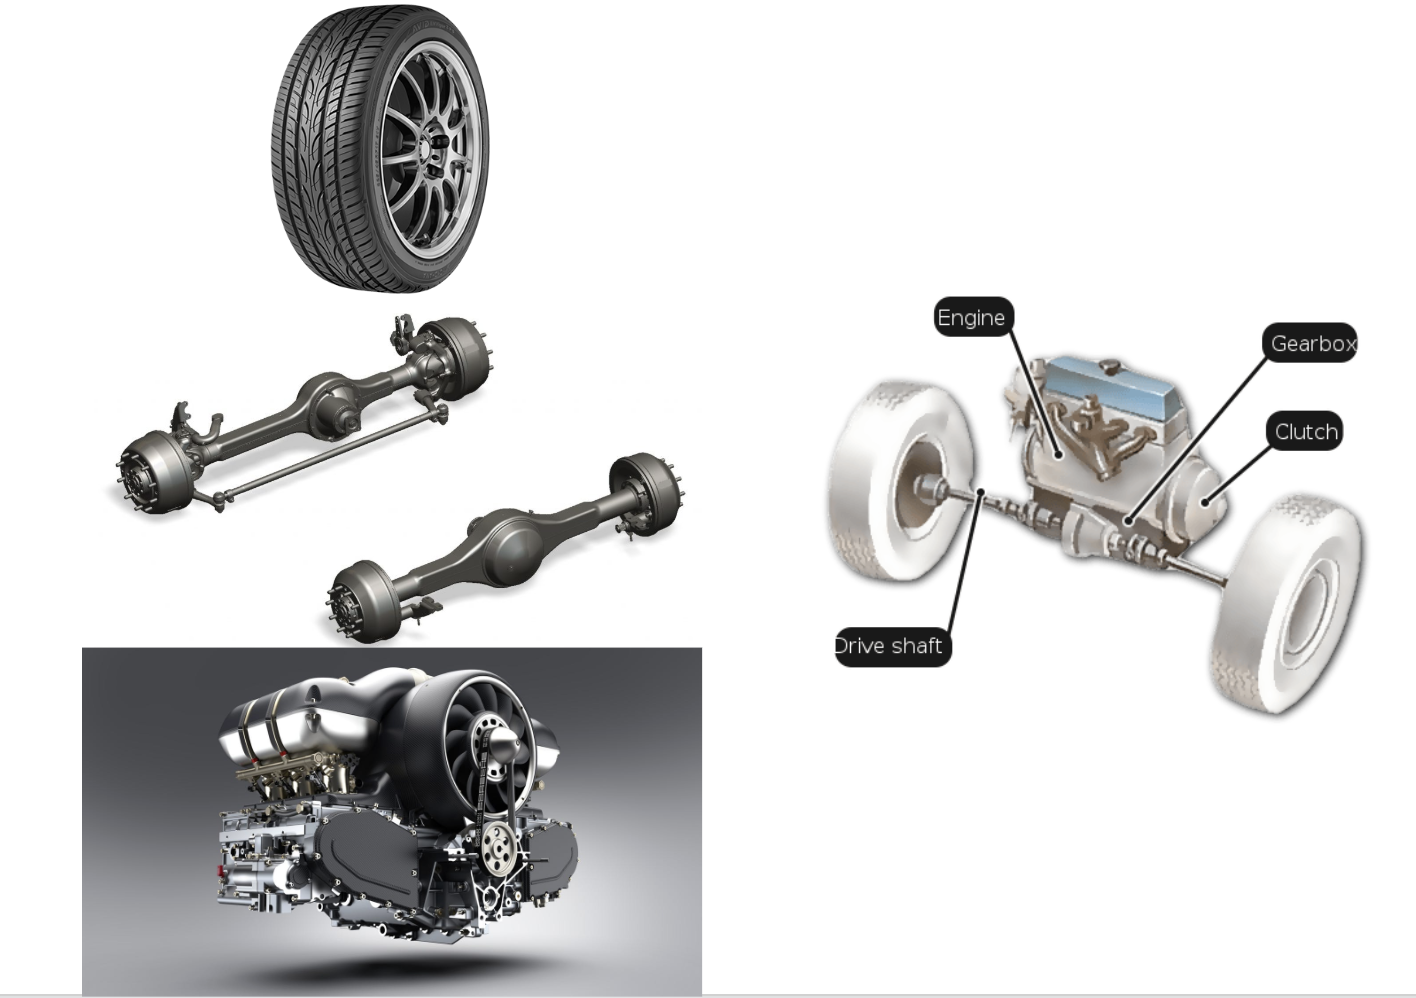
\includegraphics[width=0.5\textwidth]{images/car_example}
	\caption{Tires, engine, and axle can be combined to make the core axle-tire-engine unit of a car.}
\end{figure}

There are different ways to design each of these. They can each be made from a number of materials, and there are different sizes and varieties of each (e.g. 4 vs 6 cylinder engine, snow vs all-season tires, etc.). Furthermore, any \textit{combination} of these different varieties can be put together: we can change the type of tires we have without thinking about what type of axle or motor is in the car. 

\begin{figure}
	\centering
	
\includegraphics[width=0.5\textwidth]{images/tires.jpg}
	\caption{A variety of tires are available, and each must simply (1) be built to roll and (2) be connectable to an axle}
\end{figure}

We will now look at the benefits of this modularity in car design:

\begin{itemize}
\item \textbf{Teamwork}: Car companies can divide the work amongst multiple
  teams, and those teams won't interfere with each other as they work. One team
  can spend months developing the axle: finding the right alloy, shape, and
  weight to handle the load from the car. Another team can spend months
  developing the engine: trying out different arrangements of the cylinders or
  different numbers of cylinders. What's more, car manufacturers almost always
  outsource the production of their tires to tire manufacturers: they leave the
  decisions on the type of rubber and treads to a team totally outside of their
  company. The modularity of the car allows these teams to work totally
  separately, with the only communication between them the above list: the tire
  must roll and attach to an axle; the engine must spin the axle; and the axle
  must connect to the engine and the tires. Once the teams agree on the way they
  will bolt the systems together, they no longer have to communicate.
    
\item \textbf{Updateability}: Modularity allows car enthusiasts to upgrade and
  customize their vehicles without having to redesign the whole thing. If a
  vehicle owner wants to replace their V6 with a V8, they can do that as long as
  the connections between the motor and the rest of the vehicle are the same
  (i.e. the connection to the axle, to the fuel source, etc). If a vehicle owner
  wants to replace their all season tires for snow tires in the winter, they can
  do that as long as the connection with the rest of the vehicle is the same
  (i.e. the connection to the axle is the same).
\end{itemize}

\subsection{APIs}
\begin{definition}
An \emph{Application Programming Interface}, or API, is a contract between components in a system, expressing what each component can expect from the others. 
\end{definition}

Building on the previous section's example of a vehicle, we can consider the API between the engine manufacturer and the vehicle manufacturer. 

The engine manufacturer can expect the vehicle to:
\begin{itemize}
	\item Have an axle.
	\item Have a fuel source.
	\item Have a cooling source.
	\item Have a control system.
\end{itemize}

The vehicle manufacturer can expect the engine to:
\begin{itemize}
	\item Attach to an axle.
	\item Spin at a given revolution speed.
\end{itemize}

As we saw in the previous section, this type of contract allows division of labor between different teams working on a project to ensure that they can work independently.

Another API exists between a driver and the manufacturer: the driver can expect the car to have a:
\begin{itemize}
	\item Device to turn on/off the car.
	\item Device to steer the car.
	\item Device to accelerate the car.
	\item Device to decelerate the car.
\end{itemize}

The car maker can expect the driver to have
\begin{itemize}
	\item Arms and hands that can turn and push.
	\item Feet and legs that can press.
\end{itemize}

\begin{example}
An API between an ATM and a user. 
\end{example}

From the perspective of a user, an ATM's purpose is to take in a credit card and a specified dollar amount from a user, and output the requested amount of money. The user can expect an ATM to:
\begin{itemize}
	\item Read their credit card.
	\item Specify the card's PIN number.
	\item Specify a requested dollar amount.
	\item Output money and notify their bank of the transaction.
\end{itemize}

An ATM can expect the user to:
\begin{itemize}
	\item Have a credit card.
	\item Type with their fingers.
	\item Read and respond to prompts on the screen.
\end{itemize}

Note that a problem with the API translates to a problem with the end-product. This API doesn't guarantee that a blind person will be able to use the ATM, for example (they won't be able to read). 

\begin{example}
The API between an ATM and a bank.
\end{example}

From the perspective of a bank, an ATM's purpose is to send in credit card info and the requested dollar amount, and fulfill a user request for money only if the bank authenticates the request. 

The bank can expect an ATM to
\begin{itemize}
	\item Accurately send the bank credit card info and a PIN.
	\item Accurately send the bank the requested dollar amount.
	\item Complete the user's transaction only if the bank sends back a confirmation.
\end{itemize}

The ATM can expect the bank to
\begin{itemize}
	\item Receive credit card info and a PIN.
	\item Send back a confirmation or denial.
\end{itemize}

\section{User-oriented Design}

\subsection{Waterfall vs Iterative Design}

\begin{example}
Build the highest tower possible in 6 minutes using the following ingredients:\safemarginnote{Adapted from https://tinkerlab.com/spaghetti-tower-marshmallow-challenge/}
\begin{itemize}
	\item 10 sticks of dry spaghetti
	\item One foot of string
	\item One foot of tape
\end{itemize}
\end{example}

This activity generally demonstrates that iteration trumps pre-planning. It's faster to just try out imperfect designs than to try to wait for a perfect idea. With a 6 minute time limit, iteration tends to work out better than pre-planning. 

\begin{definition}
\emph{Waterfall design} is a development process in which each stage of development is finished before the next is started. 
\end{definition}

The components of waterfall design \footnote{adapted from https://airbrake.io/blog/sdlc/waterfall-model} are the following:
\begin{enumerate}
	\item Requirements: define what the application should do (essentially, write the API between a user and your product).
	\item Design: decide what the product will look like based on the requirements, and how it will be implemented.
	\item Implementation: build the product based on the design.
	\item Test: ensure the product works as expected.
	\item Deployment: release the product to the users.
\end{enumerate}

\begin{figure}
	\centering
	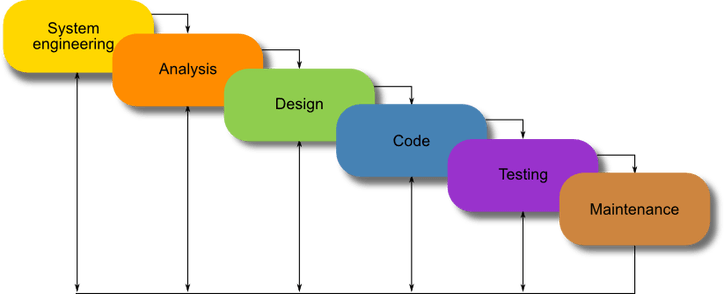
\includegraphics[width=0.5\textwidth]{images/waterfall.png}
	\caption{Waterfall design.}
\end{figure}

In waterfall design, mistakes early in the process can grow fatal. You might spend a lot of time and money going through the full waterfall and developing a final product and then realize that the requirements were wrong. Going back to a previous example, suppose you had designed an ATM thinking that users would be able to read and later found out that blind users must also be able to access the ATM. You would have to completely redesign the system, perhaps having to put speakers into the ATM so that the prompts can be read aloud to the user. 

\begin{definition}
In \emph{iterative design}, many iterations of a project are built and presented to users with the expectation that the requirements and design may need to be adjusted in further iterations. 
\end{definition}

Iterative design entails going through the same 4 steps of specifying requirements, drafting a design, implementing, then deploying. However, less time and money is invested into trying to make the first iteration perfect. The first iteration of a project might look horrible, but users will be able to tell you the fundamental flaws (such as missing requirements) before you start implementing a perfect product for the wrong problem. 

Iterative design is also used in drawing. As shown in \autoref{fig:owl}, professional artists start with a rough sketch of an object before starting to fill in details. The first iteration (top) doesn't look very good, but you might find out that you're missing basic requirements: you might be missing certain body parts, or decide you'd like to add a background or another object. By the second iteration, things look a little better, but you still might find more fundamental errors along the way. By the time you're ready to fill in all of the details in the bottom step, you're confident you're drawing the figure you want to draw. 

\begin{marginfigure}
	\centering
	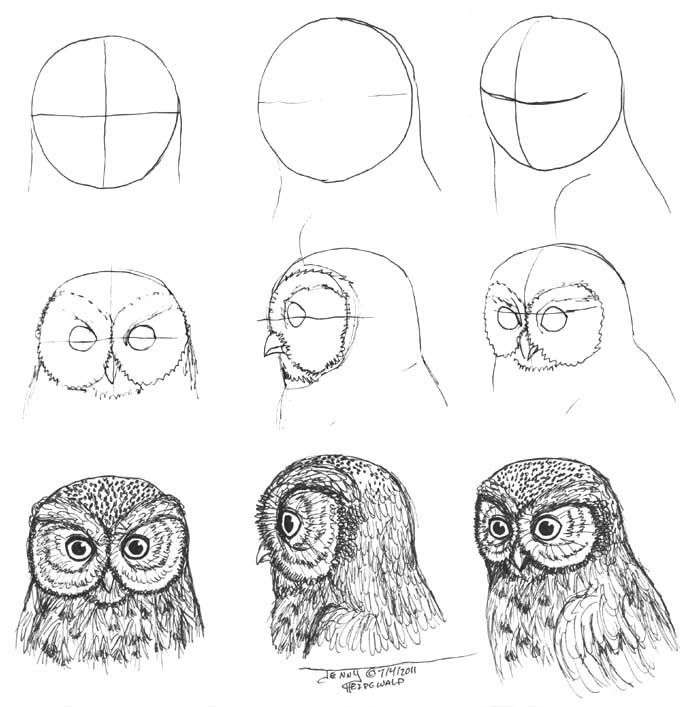
\includegraphics[width=\textwidth]{images/owl.jpg}
	\caption[Iterative drawing of an owl]{Iterative drawing of an owl. Courtesy of \url{https://www.pinterest.com/pin/469289223655955022/}.}
	\label{fig:owl}
\end{marginfigure}

\section{Testing}
Code rarely works the way we would like it to the first time around. 

\begin{definition}
A \emph{software bug}, is an error in a computer program which causes an incorrect or unexpected result, or to behave in unintended way (Wikipedia). 
\end{definition} 

Medium estimated that in 2016 approximately a trillion dollars was lost to the US economy due to software bugs. As one tangible example of the cost of bugs, in 1962 NASA's 18 million dollar Mariner 1 had to be self-destructed mid-flight because of a missing hyphen in the control code.\footnote{https://medium.com/@ryancohane/financial-cost-of-software-bugs-51b4d193f107}

For this reason, developers are always expected to carefully test the code they write to ensure there are no bugs. In addition, even relatively small software firms often have an entire team whose sole job is to test code written by the developers. Their job is to use the product in a variety of potentially unexpected ways. In essence, they try their best to break the code. The product is not ready for the market until the testing team is unable to break it, and all of its behaviors are as expected by the API for the product. 


% \section{Java interfaces}
% Recall that an API (Application Programming Interface) is a contract expressing what components in a system do. When we write code we determine \emph{how} a component works, while in an API, we only state \emph{what} it's meant to do.

% In Java, APIs\footnote{unfortunately, a set of packages that is the API of the Java language itself, and defines what classes and methods can be used "out of the box".} can be designed with a feature of the language called interface. Let's take the previous example of an ATM, its bank and its user, and consider a possible interface for the Bank:

% \begin{code}
% public interface IBank {
%     public boolean checkCard(CreditCard card, int pin);
% }
% \end{code}

% First, notice the name we chose for the interface - IBank. It is a good habit to start interface names with a capital I, and then continue in CamelCase. This helps readers know this name refers to an interface.

% Our interface has one method called checkCard, that returns a boolean. If we were implementing the method checkCard, its definition would look like this:

% \begin{code}
% public boolean isValid(CreditCard card, int pin) {
%     // some code here
% }
% \end{code}

% but in an interface, the method is only declared, with a semicolon after its declaration, and not implemented. From the declaration a user of IBank infer that checkCard receives two parameters:
% \begin{itemize}
%     \item A parameter of type int named pin
%     \item A parameter of type CreditCard named card
% \end{itemize}
% and that it returns a boolean. Someone reading the interface gets no information about \emph{how} an IBank decides whether a card is valid or not. They do know enough, however, to write their own code that needs to use the method isValid to check a card. 

% An interface by itself is not an API



% Besides their use for modularity, interfaces also help maintain another important principle in software development -- abstraction.

% \begin{definition}

% \end{definition}


% % add question about why creditcard isn't an interface? Add a question asking for such an interface?

	
	\chapter{Loop Structures}

Sometimes, it is useful to repeat an action multiple times. Maybe you want to
ask a user for their home address, if they do not provide a valid address, you
ask them for an address again. Repeating an action a number of times in this way
is a commonly used technique in programming. Structures that repeat actions are
called \emph{loop structures}.

In this chapter, we will learn a number of useful loop structures, like
\ic{while} and \ic{for} loops. We describe when to use a \ic{while} loop, and
when to use a \ic{for} loop. The chapter ends with a list of common mistakes to
avoid when writing loops.

\section{A \ic{while} loop}

\begin{definition}
A \emph{while loop} is a \emph{loop structure} that consists of the reserved
keyword \ic{while}, followed by a boolean expression enclosed in parentheses,
followed by statements typically enclosed in curly braces. These statements is
executed as long as the boolean expression remains true. If the expression
evaluates to false, the loop terminates, and the program continues.
\end{definition}

A \ic{while} loop allows us to write programs execute statements
(called the \emph{loop body}), based on a boolean expression (called the \emph{condition}). Below is an example of a simple \ic{while} loop:

\begin{code}
while (count < 20) {
  count = count+1;
  System.out.println("Count less than 20");
}
System.out.println("Count greater than, or equal to, 20");
\end{code}

\noindent The condition in this example is \ic{count > 20}. It is a boolean
expression that evaluates to either true or false. That is, \ic{count} is either
greater than \ic{20} or not. If it is, count is increased by one, and ``Count
less than 20'' is printed. Then, the program tests whether the new count is less
than 20. If it is, the count is again increased by one, and ``Count less than
20'' is printed again. Once count is greater than, or equal to, 20, ``Count
greater than, or equal to, 20'' is printed.

\begin{example}
What does the following piece of code print if \ic{x} is 98? What about if \ic{x} is 200? What about if \ic{x} is 100?

\begin{code}
while (x < 100) {
    x = x+1
    System.out.println("Not big enough...");
} 
System.out.println("Big enough!");
\end{code}

\emph{Answer}: If \ic{x} is 98, the first boolean expression will evaluate to
true, so the program will print ``Not big enough...'' Then the program will
loop, and check the condition again.  Again, it will evaluate to true, and print
``Not big enough...'' In the next iteration, x will be 100, and the conditional
will evaluate to false, and will print out ``Big enough.''

Using the same reasoning to trace the execution with \ic{x} is 200, the
following statements will be printed: ``Big enough!''.

When \ic{x} is 100, the condition is just barely big enough, so ``Big enough''
will be printed.
\end{example}

\begin{example}
How would you fill in the boolean expression to print every number downwards by 1 from the initial value of x, until x is less than 0?.

\begin{code}
while (/* Insert boolean expression here */) {
    x = x-1;
} 
\end{code}

\emph{Answer}: Insert the boolean expression x $>=$ 0. Note that it must be $>=$ rather than just $>$ since we still want to print if x is exactly 0 (only stop if x is less than 0). 
\end{example}

\begin{example}
How would you fill in the loop body to print all even numbers from 0 to 10.

\begin{code}
int x = 0;
while (x <= 10) {
    /* Insert loop body here */
} 
\end{code}

\emph{Answer}: Insert the statements:
\begin{code}
  System.out.println(x);
  x = x+2;
\end{code}
\end{example}

\section{The \ic{for} loop}
While a \ic{while} loop can express all possible loops, many while loops follow
the same pattern. Before the loop, you initialize a variable; the loop condition
involves that variable; and within the loop body, you then update that variable
in the same way. When loops involves this pattern, programmers typically write a
\ic{for} loop. Below is a \ic{for} loop that prints all the numbers from 0 to 9.

\begin{code}
for (int i = 0; i < 10; i++)
{
    System.out.println(i);
}
\end{code}

A \ic{for} loop has 4 parts, initialization, condition, change, and body. In the
above \ic{for} loop, \ic{int i = 0} is the initialization. It initializes a new
variable, \ic{i}, to be zero. Next is the condition, \ic{i < 10}. This is the
condition that describes when the loop ends. Then comes the change, \ic{i++}.
After the loop body is run, the change is run as well.  Finally is the loop
body, which in this case merely prints out \ic{i}.

Note that this loop could have been written as a while loop, shown below:
\begin{code}
int i = 0;
while (i < 10)  
{
    System.out.println(i);
    i++
}
\end{code}
%
However, programmers use a \ic{for} loop, they know that the loop structure has
the structure of requiring initialization, having a loop condition (typically
refer to the initialized variable), and having a change on each loop
iteration (typically changing the initialized variable), and having a loop body
(that typically does not change the initialized variable).

\begin{example}
What does the following piece of code print?

\begin{code}
for (int i = 10; i > 0; i--)
{
    System.out.println(i);
}
\end{code}

\emph{Answer}: 
10
9
8
7
6
5
4
3
2
1
\end{example}

\begin{example}
What does the following piece of code print?

\begin{code}
for (int j = 1; j<100; j = j*2)
{
    System.out.println(j);
}
\end{code}

\emph{Answer}: 
1
2
4
8
16
32
64
\end{example}

\begin{example}
What would you put in the initialization, condition, and change to print all
even numbers from 0 to 20 with a new line in between them?

\begin{code}
for (?; ?; ?)
{
    System.out.println(i);
}
\end{code}

\emph{Answer}:
\begin{code}
for (int i = 0; i < 20; i = i+2)
{
    System.out.println(i);
}
\end{code}
\end{example}

\section{Nested loops}
It is possible to combine loop statements in many interesting ways. Consider the following example:

\begin{code}
for (int i = 0; i < 100; i++)
{
    System.out.println("Go up to: " + i);
    for (int j = 0; j < i; j++)
    {
        System.out.println(j);
    }
}
\end{code}

\noindent For each number from 0 to 99, this code will print all the numbers up
to (and not including) it.  For example, it will start by printing \ic{0}. Then it will print \ic{0}
and \ic{1}.  Then it will print \ic{0}, \ic{1}, and \ic{2}.  This will continue
until it prints all the numbers from \ic{0} to \ic{98}.

\section{Curly braces}
So far, we have been using curly braces to enclose each of our loop bodies. These curly braces can be omitted if there is only a single statement. For example, in the snippet of code below, the first set of curly braces can be omitted, while the second cannot.

\begin{code}
int i = 0;
while (i < 10)
{
    i++;
}
i = 0;
while (i < 10)
{
    System.out.println(i);
    i++;
}
\end{code}

\noindent If all the curly braces were left out (as in the code below), the
program would complete the first loop, printing nothing. Then it would begin the
second loop, and print 0 forever..

\begin{code}
int i = 0;
while (i < 10)
    i++;
i = 0;
while (i < 10)
    System.out.println(i);
    i++;
// ^^^ Careful! This is not part of the while loop!
\end{code}

Here it is important to note that whitespace and indentation are ignored by Java. Indentation has no effect on the behavior of a program. Proper indentation is extremely important for human readability. When used incorrectly, however, misleading indentation can result in unexpected behavior.

\exercisesection

\begin{exercise}
What output is produced by the following code fragment?

\begin{code}
int i = 0;
int j = 0;
while (i < 3)
{
  j = j+i;
  System.out.println(j);
  i++;
}
\end{code}
\end{exercise}

\begin{exercise}
Convert the following loop into a \ic{for} loop.

\begin{code}
int num = 100;
while (num > 0)
{
    System.out.println(num);
    num = num / 2;
}
\end{code}
\end{exercise}

\begin{exercise}
  Write code that prints out ``hi'' 10 times, once without using loops, and once
  using loops.
\end{exercise}

\referencessection
	
 	\chapter{Methods}\label{ch:methods}

\begin{goals}
\item Write methods with parameters and non-void return types
\item Understand the components of a method
\item Study the main method in the context of the lesson
\end{goals}

% Abstraction, modularity, code-reuse, syntax, arguments and calling

% Sometimes it is useful to abstract certain computations into methods.
% In this chapter, we will be looking at how and why we can use methods to
% achieve more concise and easily-maintainable code.

Let's do a quick review of how to write a program in Java. Every line of code that runs in Java must be inside a class. A class should always start with an uppercase letter, and the name of the java file should be the same as the classname but with ``.java" at the end. 

Every Java program needs a \ic{main()} method that looks like this:

\begin{code}
public static void main(String[] args)
\end{code}

For example, our hello world program from the beginning of the semester is 

\begin{code}
class MyClass {
  public static void main(String[] args) {
    System.out.println("Hello World");
  }
}
\end{code}

Any code inside the \ic{main()} method is executed when the program is run. But after all this time, we still don't know what a method is! Let's fix that. 

\section{Methods}

\subsection{Introduction}

A \emph{method} is a block of code which only runs when it is called. You can pass data, known as parameters, into a method. Methods are used to perform certain actions, and they are also known as \emph{functions}.

We use methods in order to define code once, and use it many times. They help organize code and make debugging much faster. We will understand the benefits more clearly in coming lectures and exercises. 

A method must be declared within a class. It is defined with the name of the method, followed by parentheses (). Java provides some pre-defined methods, such as \ic{System.out.println()}, but you can also create your own methods. Here is an outline for making a method named ``myMethod" within a class called ``MyClass": 

\begin{code}
class MyClass {
  public static void myMethod() {
    // code to be executed
  }
}
\end{code}

\ic{myMethod()} is the name of the method. Public means that code outside of the MyClass class will be able to run the method. Static means that the method belongs to the MyClass class and not an object of the MyClass class. We won't explain in detail exactly these definitions of "public" and "static" mean until later in the course. For now, you should just remember to write ``public static" at the start of every method declaration. \ic{void} means that this method does not have a return value. We will understand what this means later in this chapter. 

Now let's define what the method should do. Let's make our method print \ic{Hello World}. 
\begin{code}
class MyClass {
  public static void myMethod() {
    System.out.println("Hello World");
  }
}
\end{code}

We've successfully written a method! But remember that every Java program needs a \ic{main()} method, since the \ic{main()} method is what Java tries to execute when you run the program. Let's see the error Java throws if we \emph{don't} have a main method. Save this file as ``MyClass.java" (filename must match class name!) within a new folder called ``Methods" in your ``CS103" folder. Now compile, and try running the program. You should see the error \ic{Static Error: This class does not have a static void main method accepting String[].} Big lesson: only code within the main method actually gets executed. If we want to run the code in the \ic{myMethod()} function, we need to \emph{call} the \ic{myMethod()} method from the \ic{main()} method. To call a method in Java, write the method's name followed by two parentheses (). As always, your statement should end in a semicolon. The full program should look like this: 

\begin{code}
class MyClass {
  public static void myMethod() {
    System.out.println("Hello World");
  }

  public static void main(String[] args) {
    myMethod();
  }
}
\end{code}

Compile and run this code, and you should see the output ``Hello World". 

Methods can be run multiple times. Try calling the \ic{myMethod} method 3 times from the \ic{main()} method:\marginnote{It's often helpful to trace through the code with your finger to understand the order of execution. Although \ic{myMethod()} comes before the \ic{main()} method in this program, when you run a program Java always just executes the \ic{main()} method. Try stepping through this example with your finger, showing the order in which Java looks at each piece of the program. What would happen if we had no code in our \ic{main()} method?}

\begin{code}
class MyClass {
  public static void myMethod() {
    System.out.println("Hello World");
  }

  public static void main(String[] args) {
    myMethod();
    myMethod();
    myMethod();
  }
}
\end{code}

This should print ``Hello World" 3 times, separated by newlines. 

You can define as many methods as you want in a Java program as long as they have different names. Let's see this with an example: 

\begin{example}
Fill in the blanks within the main method of the following code to make it print ``Hello" then ``World" by calling the two methods \ic{printHello} and \ic{printWorld}. 
\begin{code}
class MyClass {

    public static void printHello() {
        System.out.print("Hello ");
    }
    
    public static void printWorld() {
        System.out.println("World");
    }

    public static void main(String[] args) {
        ______________ // call method to say "Hello"
        ______________ // call a method to say "World"
    }
}
\end{code}
\noindent \emph{Answer}:
\begin{code}
    printHello();
    printWorld();
\end{code}
\end{example}

\marginnote{Not only can you have as many methods as you want in a Java program, you can also put them in any order. Try typing the above into DrJava and make sure it runs and outputs what you expect. Then try moving the \ic{main()} method before the \ic{printHello()} and \ic{printWorld()} methods. Ensure it runs exactly the same.}

\subsection{Parameters} 

Information can be passed to methods as \emph{parameters}. Parameters act as variables inside the method. Parameters are specified after the method name, inside the parentheses. You can add as many parameters as you want, just separate them with a comma.

The following example has a method called \ic{printFullName} that takes a String called \ic{firstName} as parameter. 

\begin{code}
class MyClass {
  public static void printFullName(String firstName) {
    System.out.println(firstName + " Reyes");
  }

  public static void main(String[] args) {
    printFullName("Liam");
    printFullName("Jenny");
    printFullName("Anja");
  }
}
\end{code}

Save, compile, and try running it. 

\marginnote{Note that we can name parameters whatever we want. How would you rewrite the \ic{printFullName()} method to use the parameter name \ic{foreName} instead of \ic{firstName}?}When a parameter is passed to the method, it is called an \emph{argument}. So, from the example above: fname is a \emph{parameter}, while Liam, Jenny and Anja are \emph{arguments}. When the method is called, we pass along a first name as an argument and the method prints out the person's name with a last name of ``Reyes" appended. When we pass in ``Liam" as an argument to the \ic{printFullName()} method, Java makes a new variable called \ic{firstName} to be used within the \ic{printFullName()} method body. So whenever we see \ic{firstName} during the method call with argument ``Liam", Java really thinks of it as the String ``Liam". When we pass in the argument ``Jenny", Java sets \ic{firstName} to ``Jenny". 

Now let's try an example with multiple parameters:

\begin{example}

Fill in the two blanks in the code below to print the message ``Liam is 5" ``Jenny is 8" and ``Anja is 31"
\begin{code}
class MyClass {
  public static void printNameAndAge(String firstName, int age) {
    System.out.println(firstName + " is " + ____);
  }

  public static void main(String[] args) {
    printNameAndAge("Liam", 5);
    printNameAndAge("Jenny", 8);
    // call a method to print the message "Anja is 31":
    ____________________ 
  }
}
\end{code}
\end{example}

\marginnote{What are the parameters and what are the arguments in the above example calling the \ic{printNameAndAge()} example?} Note that when you are working with multiple parameters, the method call must have the same number of arguments as there are parameters, and the arguments must be passed in the same order.

\subsection{Return types}
The void keyword, used in the examples above, indicates that the method should not return a value. If you want the method to return a value, you can specify a data type (such as int, char, etc.) instead of void, and use the return keyword\marginnote{when we write ``return" followed by a space then an expression, the method will immediately spit out the expression so it can be used by whatever code called the method} inside the method: 

\begin{code}
class MyClass {
  public static int addFive(int x) {
    return 5 + x;
  }

  public static void main(String[] args) {
    System.out.println(addFive(3));
  }
}
\end{code}

Here's another example with a method taking two arguments:

\begin{code}
class MyClass {
  static int takeSum(int x, int y) {
    return x + y;
  }

  public static void main(String[] args) {
    System.out.println(takeSum(5, 3));
  }
}
\end{code}

\marginnote{What does the takeSum method do? What is the output of the full example program?}

Whereas our previous examples printed information from within our methods, now we are getting the output of a method in the main method and printing its value from there. 

Non-void return types also allow us to store results from methods in variables. Using variables to store the return value from methods is recommended, since it makes code easier to read and maintain. In the following example, we store the return value of \ic{takeSum(5, 3)} in the integer \ic{z}:

\begin{code}
class MyClass {
  static int takeSum(int x, int y) {
    return x + y;
  }

  public static void main(String[] args) {
    int z = takeSum(5, 3);
    System.out.println(z);
  }
}
\end{code}

\subsection{Endless possibilities} 

All of the concepts we've learned so far can be applied in methods, from control structures to loops to arrays. Here's an example of a method that makes use of if...else: \marginnote{Note that in all of the examples so far our methods start with a verb: the method name says what the method does. ``printHello" printed ``Hello", ``printFullName" printed a person's full name, ``addFive" added five to a number, ``checkAge" checked a person's age to see whether to grant access, and ``getSmaller" got the smaller of two numbers. Try to always start with a verb when you're deciding how to name your methods. For example, what might you call a method meant to take a number from 0-100 as argument and return the number's corresponding letter grade from A-F?}

\begin{code}
class MyClass {

  // Create a checkAge() method with an integer variable called age
  public static void checkAge(int age) {

    // If age is less than 18, print "access denied"
    if (age < 18) {
      System.out.println("Access denied - You are not old enough!");

    // If age is greater than 18, print "access granted"
    } else {
      System.out.println("Access granted - You are old enough!");
    }

  }

  public static void main(String[] args) {
    checkAge(20); // Call the checkAge method and pass along an age of 20
  }
}
\end{code}

What does the code above output?

\begin{example}
Fill in the blanks in the code below to make a method that returns the smaller of two numbers:

\begin{code}
class MyClass {

  public static int getSmaller(int num1, int num2) {
    int ret;
    if (num1 < num2) {
        ret = ____;
    }
    else {
        ret = ____;
    }
    return ret; 
  }

  public static void main(String[] args) {
    System.out.println(getSmaller(1,2));
  }
}
\end{code}

\noindent \emph{Answer}:

\textbf{1st blank:} num1

\textbf{2nd blank:} num2
\end{example}

Let's use loops!

\begin{example}
Fill in the blanks in the code below to make a method that adds all numbers in an array and calls it on \ic{\{1, 2\}} to return \ic{3}. 

\begin{code}
class MyClass {
  // make sure the parameter numArray's type is integer array
  public static int addNumbers(____ numArray) {
    int sum = 0;
    for (int i=0; i<numArray.length; i++) {
      sum = sum + numArray[i]; // print i
    }
    return sum; 
  }

  public static void main(String[] args) {
    int[] inputArray = {1,2};
    int sum = ______; // call the addNumbers method on inputArray
    System.out.println(sum);
  }
}
\end{code}

\noindent \emph{Answer}:

\textbf{1st blank:} int[] 

\textbf{2nd blank:} addNumbers(inputArray)
\end{example}


% We will first look at some code that does not use methods and identify some
% problems with this code. We will then, in Section \ref{sec:methods},
% introduce what a method is, including how to define and use them.
% In Sections \ref{sec:abstraction} and \ref{sec:modularity}, we will
% then talk about how we can use methods to improve the problems that
% we noticed with our code. In particular, in Section \ref{sec:abstraction},
% we talk about how methods allow us to abstract some of our code to get
% more concise and maintainable code, and in Section \ref{sec:modularity},
% we talk about how methods allow us to divide our code up into chunks
% that we can consider in isolation, allowing us to manage and maintain
% our code more easily. We'll finish the chapter by getting a more concrete understanding of how to write programs using methods. 

% Let us consider the following problem:

% We have a class of nine students, split up into three groups of three.
% We want to report the maximum score for each group.
% %as well as the maximum score for the students overall.
% We will use the variable names \ic{group1s1}, \ic{group1s2}, and \ic{group1s3}
% to refer to the three scores achieved by the students in Group 1, and we will use
% a similar naming convention for the variable names for the scores achieved by
% students in Group 2 and Group 3.

% The following snippet of code computes the maximum score in Group 1, storing
% the result in \ic{group1Max}.
% \begin{code}
% int group1Max = group1s1;
% if (group1s2 > group1Max) {
%   group1Max = group1s2; 
% }
% if (group1s3 > group1Max) {
%   group1Max = group1s3; 
% }
% \end{code}

% If we now wish to extend this to compute the maximum score for each group,
% we can copy the code and rename the variables to achieve the following
% code:
% \begin{code}
% int group1Max = group1s1;
% if (group1s2 > group1Max) {
%   group1Max = group1s2; 
% }
% if (group1s3 > group1Max) {
%   group1Max = group1s3; 
% }

% int group2Max = group2s1;
% if (group2s2 > group1Max) {
%   group2Max = group2s2; 
% }
% if (group2s3 > group2Max) {
%   group2Max = group2s3; 
% }

% int group3Max = group3s1;
% if (group3s2 > group3Max) {
%   group3Max = group3s2; 
% }
% if (group3s3 > group3Max) {
%   group3Max = group3s3; 
% }
% \end{code}

% \noindent There are a couple of things about the process of getting this resulting code
% that aren't particularly ideal.
% The first is that it is very easy to make a mistake when copying the code and renaming
% the variables. For example, we might have missed renaming \ic{group1Max} to \ic{group3Max}
% in the computation of the maximum score for Group 3, leading us to compute an incorrect maximum
% value in some cases.

% The second issue is that there is a lot of redundancy.
% If we look at the code, we can notice that there seem to be a lot of redundant parts
% across the code for the three different groups.
% If we had ended up with the wrong computation initially and needed to fix it
% later, then we would have to make sure we fixed it everywhere, leading to repeated work and the
% possibility that we didn't fix one of the copies. For example, if we initially started out with
% \ic{group1s3 < group1Max} instead of \ic{group1s3 > group1Max}, and then copied and renamed variables
% to compute the maximum scores for the other groups, we would end up with the code below:

% \begin{code}
% int group1Max = group1s1;
% if (group1s2 > group1Max) {
%   group1Max = group1s2;
% }
% if (group1s3 < group1Max) {
%   group1Max = group1s3;
% }

% int group2Max = group2s1;
% if (group2s2 > group1Max) {
%   group2Max = group2s2;
% }
% if (group2s3 < group2Max) {
%   group2Max = group2s3;
% }

% int group3Max = group3s1;
% if (group3s2 > group3Max) {
%   group3Max = group3s2;
% }
% if (group3s3 < group3Max) {
%   group3Max = group3s3;
% }
% \end{code}

% To fix our code, we would not only have to replace \ic{group1s3 < group1Max} with
% \ic{group1s3 > group1Max}, but we would also need to replace \ic{group2s3 < group2Max} with
% \ic{group2s3 > group2Max} and \ic{group3s3 < group3Max} with \ic{group3s3 < group3Max}.

% \section{Methods}\label{sec:methods}
% In Java, we can use abstractions in our code in the form of \emph{methods}.
% Methods contain bits of code that may compute things using \emph{arguments}
% that are passed into the method.

% An example of the syntax for a \emph{method definition} is given below:
% \begin{code}
% public bool negate(bool arg) {
%   return !arg; // method body
% }
% \end{code}
% We can identify the different components of the method definition:
% \begin{itemize}
% \item  The \emph{access modifier} of the method is \ic{public},
% \item the \ic{bool} before \ic{negate} gives the \emph{return type} of the method
% \item \ic{negate} is the \emph{name of the method},
% \item \ic{arg} is the \emph{name of the first argument/parameter} of the method,
% \item the \ic{bool} before \ic{arg} it is the \emph{type} of the \ic{arg} parameter,
% \item and the code between the curly braces is the method \emph{body}.
% \end{itemize}
% Inside the method body, there is code that may use the arguments of the method.
% In the example above, the body only consists of the \ic{return} statement.
% The \ic{return} statement is followed by something of the return type of the method.
% This expression, after being evaluated, gives the \emph{return value} of the method.
% As soon as a \ic{return} statement is encountered, a method finishes its execution.
% \emph{Access modifiers} will be described later on when we talk about Classes,
% but note that if an access modifier is omitted, it the method has the \emph{default} modifier.

% Other important terms to note are as follows:
% The \emph{parameter list} of a method consists of the types of its parameters in the
% order they are given in the method definition.
% For the above method, it is simply \ic{bool}.
% The \emph{method signature} consists of the method name and parameter list.
% For the above method, it is \ic{negate(bool)}.
% A method is identified by its method signature.

% \begin{example}
% Consider the following method:
% \begin{code}
% int squareSum(int arg0, int arg1) {
%   int res = arg0 + arg1;
%   return res * res;
% }
% \end{code}
% Give the following for the method:
% \begin{itemize}
% \item Access modifier
% \item Return type
% \item Arguments
% \item Method signature
% \end{itemize}

% \noindent \emph{Answer}: 
% \begin{itemize}
% \item Access modifier: default
% \item Return type: \ic{int}
% \item Arguments: \ic{arg0}, \ic{arg1}
% \item Method signature: \ic{squareSum(int, int)}
% \end{itemize}
% \end{example}

% \begin{example}
% Consider the following method:
% \begin{code}
% private void mystery (int age, String name) {
%   if (age >= 18) {
%     System.out.println(name);
%   }
% }
% \end{code} 
% Give the following for the method:
% \begin{itemize}
% \item Access modifier
% \item Return type
% \item Name
% \item Parameter list
% \end{itemize}

% \noindent \emph{Answer:}
% \begin{itemize}
% \item Access modifier: \ic{private}
% \item Return type: \ic{void}
% \item Name: \ic{mystery}
% \item Parameter list: \ic{int, String}
% \end{itemize}

% \end{example}

% We may \emph{call} or \emph{invoke} the above \ic{negate} method from elsewhere in the code by,
% for example, using \ic{negate(true)} if we want to call \ic{negate} with argument
% \ic{true}.
% We must specify the name of the method that we wish to call, followed by the arguments
% that we wish to call it on, separated by commas if there are more than one.
% The arguments provided in the call must correspond to the types of the arguments
% specified in the method definition: if the method definition has the type \ic{bool}
% for its first argument, then the first argument supplied in the call should also be
% of type \ic{bool}, and if the definition has the type \ic{int} for its second argument,
% then the first argument in the call should also be of type \ic{int}, and so on.
% A method invocation evaluates to the return value it computes, where this
% computation happens with the actual arguments
% given in the call substituted for the arguments specified in the definition, so in
% this case, the invocation \ic{id(true)} evaluates to \ic{false}.
% A method invocation has the same type as its return type, which in this case, is \ic{bool}.

% So, for example, we can do something like in following code snippet:
% \begin{code}
%   bool f = negate(true);
%   bool t = negate(negate(true));
% \end{code}
% After executing the above code, the variable \ic{f} contains the value \ic{false}
% and the variable \ic{t} contains the value \ic{true}.

% Note that we can also have methods that do not return anything. Such
% methods have \ic{void} return types. They may contain a \ic{return}
% statement with no expression following \ic{return}.
% Calls to these methods cannot be used inside of other expressions.
% Two examples of methods with \ic{void} return types are below:
% \begin{code}
% public void printSum(double a, double b) {
%   System.out.println(a + b);
% }
% \end{code}

% \begin{code}
% public void printBigger(double a, double b) {
%   if (a > b) {
%     System.out.println(a);
%     return;
%   }
%   System.out.println(b);
% }
% \end{code}
% Note that the latter example only ever prints the value of either \ic{a} or \ic{b} but
% never both because
% the \ic{return} statement finishes the execution of the method.

% Some methods also do not take any arguments at all. One such example is below:
% \begin{code}
% public int constantOne() {
%   return 1;
% }
% \end{code}
% \noindent This method can be called using \ic{constantOne()}.

% \begin{example}
% What value does \ic{res} have after the following code snippet is executed?
% \begin{code}
% int res = constantOne() + constantOne();
% \end{code}
% \emph{Answer}: The value of \ic{res} is 2.
% \end{example}.

% Note that for every method that does not have a \ic{void} return type,
% for every possible control-flow path through the method body,
% there must be a \ic{return} statement that is eventually reached.
% For example, the following method does not meet this requirement
% because when \ic{arg} is \ic{false}, the \ic{return} statement is not
% reached:
% \begin{code}
% public int twoIfTrue(bool arg) {
%   if (arg) {
%     return 2;
%   }
% }
% \end{code}

% \begin{example}
% Consider the following method:
% \begin{code}
% public void mystery (bool arg0, int arg1) {
%   if (arg0) {
%     return -1 * arg1;
%   }
%   return arg0;
% }
% \end{code}

% \noindent What do each of the following evaluate to?
% \begin{itemize}
% \item \ic{mystery(true, -2)}
% \item \ic{mystery(true, 0)}
% \item \ic{mystery(true, 4)}
% \item \ic{mystery(false, -2)}
% \item \ic{mystery(false, 0)}
% \item \ic{mystery(false, 4)}
% \end{itemize}

% \noindent \emph{Answer:}
% \begin{itemize}
% \item \ic{mystery(true, -2)} evaluates to 2
% \item \ic{mystery(true, 0)} evaluates to 0
% \item \ic{mystery(true, 4)} evaluates to $-4$
% \item \ic{mystery(false, -2)} evaluates to $-2$
% \item \ic{mystery(false, 0)} evalutes to 0
% \item \ic{mystery(false, 4)} evalutates to 4
% \end{itemize}

% \noindent What does the method do?

% \noindent \emph{Answer:} It negates its second argument
% \ic{arg1} whenever its first argument \ic{arg0} is
% \ic{true} and otherwise just returns its second argument
% \ic{arg1}.
% \end{example}

% \begin{example}
% How many methods can be called by the following method?
% What do you think each of their return types and parameter lists are?

% \begin{code}
% public void sayHello(int times, String name, String day) {
%   if (shouldStop(times))
%     return;
%   String hello = getHelloStr(name, day);
%   System.out.print.ln(hello);
%   sayHello(times - 1, name, day);
% }
% \end{code}
% \noindent \emph{Answer:}
% Three methods can be called: \ic{shouldStop}, \ic{getHelloStr} and \ic{sayHello}.

% The return type of \ic{shouldStop} is \ic{bool}, and it has parameter list \ic{int}.
% The return type of \ic{getHelloStr} is \ic{String}, and it has parameter list \ic{String, String}.
% The return type of \ic{sayHello} is \ic{void}, and it has parameter list \ic{int, String, String}.
% \end{example}

% \begin{example}
% Write a method with signature \ic{printInOrder(int, int, int)} that takes
% three \ic{int}s \ic{a}, \ic{b}, and \ic{c} as arguments and prints them out,
% one per line, in increasing order. E.g. \ic{printInOrder(5, 9, 7)} should output the following:
% \begin{code}
% 5
% 7
% 9
% \end{code}

% \noindent \emph{Answer:}
% A possible solution is the following:
% \begin{code}
% public void printInOrder(int a, int b, int c) {
%   int smallest = a;
%   int middle = b;
%   int biggest = c;
%   if (smallest > middle) {
%     int tmp = smallest;
%     smallest = middle;
%     middle = tmp;
%   }
%   if (smallest > biggest) {
%     int tmp = smallest;
%     smallest = biggest;
%     biggest = tmp;
%   }
%   if (middle > biggest) {
%     int tmp = middle;
%     middle = biggest;
%     biggest = tmp;
%   }
%   System.out.println(smallest);
%   System.out.println(middle);
%   System.out.println(biggest);
% }
% \end{code}
% \end{example}

\subsection{The main method}
To tie things together, let's go back to the main method for the Hello World program that we've seen so many times but never understood.

\begin{code}
class MyClass {
  public static void main(String[] args) {
    System.out.println("Hello World");
  }
}
\end{code}

In this case, the MyClass class has only one method, and it is the (required) main() method. ``public static" must be written for any method (at least for now). Main methods always have ``void" return types because Java simply runs them and doesn't store any values. And the parameter ``String[] args" is a parameter that always must be there for a main method. This String array will be filled with the words that you type after ``run MyClass" when running your program. We will get more practice with this in the next semester.  

\subsection{Overloading (Optional)}

With method \emph{overloading}, multiple methods can have the same name with different parameters. This is useful in a few cases.

For one, consider the following code that includes both a \ic{addTwoInts()} and a \ic{addTwoDoubles()} method so that we can add both integers and doubles in our \ic{main()} method. 

\begin{code}
public class MyClass{
  static int addTwoInts(int x, int y) {
    return x + y;
  }

  static double addTwoDoubles(double x, double y) {
    return x + y;
  }

  public static void main(String[] args) {
    int myNum1 = addTwoInts(8, 5);
    double myNum2 = addTwoDoubles(4.3, 6.26);
    System.out.println("int: " + myNum1);
    System.out.println("double: " + myNum2);
  }
}
\end{code}

Instead of defining two methods that should do the same thing (add two numbers), it is better to overload one. In the example below, we overload a single method called ``addNumbers" to work for both int and double:

\begin{code}
public class MyClass{
  static int addTwoNumbers(int x, int y) {
    return x + y;
  }

  static double addTwoNumbers(double x, double y) {
    return x + y;
  }

  public static void main(String[] args) {
    int num1 = addTwoNumbers(8, 5);
    double num2 = addTwoNumbers(4.3, 6.26);
    System.out.println("int: " + num1);
    System.out.println("double: " + num2);
  }
}
\end{code}



Because of this, we can actually have methods with the same name (in the same
Class) as long as they have different parameter lists.

For example, we can have the following two methods because
one has signature \ic{printBigger(double, double)} and the other
has signature \ic{printBigger(int, int)}:
\begin{code}
public void printBigger(double a, double b) {
  if (a > b) {
    System.out.println(a);
    return;
  }
  System.out.println(b);
}
public void printBigger(int a, int b) {
  if (a > b) {
    System.out.println(a);
    return;
  }
  System.out.println(b);
}
\end{code}
In this case, we say that the \ic{printBigger} method is \emph{overloaded}.

However, we cannot have the following two methods because they both have the
same signature \ic{twoIfTrue(bool)}:
\begin{code}
public int twoIfTrue(bool arg) {
  if (arg) {
    return 2;
  }
}
public double twoIfTrue(bool arg) {
  if (arg) {
    return 2.0;
  }
}
\end{code}

\begin{example}
Consider the following two methods that we have seen in previous
examples:
\begin{code}
private void mystery (int age, String name) {
  if (age >= 18) {
    System.out.println(name);
  }
}
public void mystery (bool arg0, int arg1) {
  if (arg0) {
    return -1 * arg1;
  }
  return arg0;
}
\end{code}
Are we allowed to have both of these methods together (in the same Class)?
Why or why not?

\noindent \emph{Answer:}
We are allowed to have both of these methods together because they have
different signatures. One has signature \ic{mystery(int, String)}
and the other has signature \ic{mystery(bool, int)}.
\end{example}

\begin{example}
Which of the following are valid overloadings?

\noindent A:
\begin{code}
public int absValue(int x) {
  if (x < 0) {
    return x * -1;
  }
  return x;
}
public double absValue(int x) {
  if (x < 0) {
    return 0.0 - x;
  }
  return x - 0.0;
}
\end{code}

\noindent B:
\begin{code}
public int absValue(int x) {
  if (x < 0) {
    return x * -1;
  }
  return x;
}
public double absValue(double x) {
  if (x < 0) {
    x = 0.0 - x;
  }
  return x;
}
\end{code}

\noindent C:
\begin{code}
public int absValue(int x) {
  if (x < 0) {
    return x * -1;
  }
  return x;
}
public int absValueX(int x) {
  if (x < 0) {
    return x * -1;
  }
  return x;
}
\end{code}

\noindent \emph{Answer:}
\begin{itemize}
\item A is not a valid overloading because both methods have the same signature.
\item B is a valid overloading because both methods have different signatures.
\item C is valid code, but this is not a valid overloading. It is not overloading at all because the methods have different names.
\end{itemize}
\end{example}

\subsection{Methods Summary}
In summary, every method definition has the following:
\begin{itemize}
\item An access modifier (if not explicitly stated, this will be the \emph{default} modifier)
\item A return type (possibly \ic{void})
\item A name
\item A (possibly empty) list of parameter types and names that can be passed to the method when it is called
\item A body
\item A return statement reached on every control path in the body, where each \ic{return} is followed by an
expression of the method's return type (unless the return type is \ic{void})
\end{itemize}
Each method is identified by its signature, so you may have methods with the same name but different parameter lists.

\section{Abstraction}\label{sec:abstraction}
Let us now return to our problem of finding the maximum scores for each
of the three groups.
The code for each of the three groups, though similar, have different variable names;
however, this is the only way in which they are different.
The process of distilling the similarity among different pieces of code is
the process of \emph{abstraction}.
In this case, we would like to \emph{abstract} away the details of
each copy to achieve a piece of code that describes all of their behavior.

After abstracting away the variable names, the code for each group is such that,
if we use the appropriate variable names for the students in the group
instead of \ic{x}, \ic{y}, and \ic{z}, that the following code snippet
would describe all of the three different operations, with
\ic{max} storing the desired result:
\begin{code}
int max = x;
if (y > max) {
  max = y; 
}
if (z > max) {
  max = z;
}
\end{code}
We can wrap this code snippet up in a method definition
that returns the value we care about:
\begin{code}
public int max3(int x, int y, int z) {
  int max = x;
  if (y > max) {
    max = y;
  }
  if (z > max) {
    max = z;
  }
  return max;
}
\end{code}

If we use this method in place of the redundant code,
our original code that compute the maximum scores for each of the three
groups then becomes as follows:
\begin{code}
int group1Max = max3(group1s1, group1s2, group1s3);
int group2Max = max3(group2s1, group2s2, group2s3);
int group3Max = max3(group3s1, group3s2, group3s3);
\end{code}
This resulting code is much more concise and is an example
of \emph{code reuse}, where the same exact code
(i.e. the code inside the body of \ic{max3}) is being reused
in several places. This code is also perhaps easier to understand
if you know that \ic{max3} simply calculates the maximum
of its three arguments. In the original code, after
going through the code for one of the groups
and realizing that it computes a maximum, you
would have to go through the calculations of the other
groups to make sure that they also compute a maximum.
Here, it is easy to see that the same computation is happening
for each group (but with different inputs).

We might further notice that both of the conditional statements
in the \ic{max3} method
compute very similar things (i.e. the maximum of two numbers),
and might perform further abstraction to achieve the following
method:
\begin{code}
int max2(int x, int y) {
  int max = x;
  if (y > max) {
    max = y; 
  }
}
\end{code}

We can then adjust our \ic{max3} method to call this one:
\begin{code}
int max3(int x, int y, int z) {
  return max2(max2(x, y), z);
}
\end{code}

Note that we do not need to change our code
for computing \ic{group1Max}, \ic{group2Max},
or \ic{group3Max} in order to use the method
\ic{max2}. The changes to \ic{max3} are sufficient.

\section{Modularity (Optional)}\label{sec:modularity}
Let us again consider the case in which our calculation of the maximum
score is incorrect because we used \ic{<} instead of \ic{>} in
the last comparison. Let us assume that we are still using the
version of \ic{max3} that does not call \ic{max2}, but
we mistakenly have the comparison \ic{z < max} instead of
\ic{z > max} in our method:
\begin{code}
public int max3(int x, int y, int z) {
  int max = x;
  if (y > max) {
    max = y;
  }
  if (z < max) {
    max = z;
  }
  return max;
}
\end{code}

In order to fix, this we simply need to change \ic{z < max}
to \ic{z > max} once. The code that calculates
the values of \ic{group1Max}, \ic{group2Max},
and \ic{group3Max} by calling \ic{max3} is fixed by this
one change because for all the groups, we call the
same method. Here we have achieved a \emph{separation of concerns}
in the two parts of our code:
\begin{itemize}
\item We have one part of our code (the \ic{max3} method)
that is concerned with finding the maximum of three \emph{arbitrary}
numbers, but it is not concerned with \emph{which} numbers
specifically for which it is finding the maximum.
\item We have another part that
is concerned with computing the maximum scores for each group,
\emph{given that} we have some other code that
can calculate the maximum of three numbers, but it is
not concerned with \emph{how} this maximum is found,
as long as it is done correctly
\end{itemize}

This separation of concerns is referred to as \emph{modularity},
and we can regard the code inside of different methods as
being in different \emph{modules}.
We have already seen that modularity can allow us to do
things like fix bugs in one part of our code without having
to touch other parts of our code.

Modularity also lets us do other things, like naturally
divide up labor. If you wanted to split up the work
of writing a program that finds the maximum of each
group's three scores with a friend,
you might volunteer to write the code that deals with
finding the maximum scores for each group provided that
your friend writes code that finds the maximum of three numbers
contained in a method with signature \ic{max3(int, int int)} that returns
an \ic{int} that is the maximum of its three \ic{int} arguments.

Given that you know your friend will write such a \ic{max3}
method, you can, without seeing your friend's code,
write the following code (that we have already seen):
\begin{code}
int group1Max = max3(group1s1, group1s2, group1s3);
int group2Max = max3(group2s1, group2s2, group2s3);
int group3Max = max3(group3s1, group3s2, group3s3);
\end{code}

\noindent Once your friend finishes writing \ic{max3}, then your code
should work as expected. 

An advantage of modularity is that it is not necessary
to know the details of how the modules that you use
are implemented nor used.
In the above example, you do not need to know how exactly your
friend implements \ic{max3} (maybe it calls \ic{max2}
and maybe it does not) and your friend does not need to
know how you use \ic{max3} (maybe you also use it to
find the maximum of the three maximum scores and maybe
you do not).

\begin{example}
What would you add to the following code to calculate
the maximum of \ic{group1Max}, \ic{group2Max},
and \ic{group3Max} and store it in \ic{allGroupMax}?

\begin{code}
int group1Max = max3(group1s1, group1s2, group1s3);
int group2Max = max3(group2s1, group2s2, group2s3);
int group3Max = max3(group3s1, group3s2, group3s3);
\end{code}

\noindent \emph{Answer:}
\begin{code}
int group1Max = max3(group1s1, group1s2, group1s3);
int group2Max = max3(group2s1, group2s2, group2s3);
int group3Max = max3(group3s1, group3s2, group3s3);
// added code below:
int allGroupMax = max3(group1Max, group2Max, group3Max);
\end{code}
\end{example}

\begin{example}
Consider the case where not only do you
want to compute the maximum scores for each group
for Group 1, Group 2, and Group 3, but you
also want to do the same for Group 4 and Group 5.
Unfortunately, while Group 4 and Group 5 also have
three scores per group (\ic{group4s1}, \ic{group4s2},
\ic{group4s3}, \ic{group5s1}, \ic{group5s2},
and \ic{group5s3}), these scores are all \ic{double}s
rather than \ic{int}s.

You want write the following code:
\begin{code}
int group1Max = max3(group1s1, group1s2, group1s3);
int group2Max = max3(group2s1, group2s2, group2s3);
int group3Max = max3(group3s1, group3s2, group3s3);
double group4Max = max3(group4s1, group4s2, group4s3);
double group5Max = max3(group5s1, group5s2, group5s3);
\end{code}

What code do you ask your friend to write
so that your code works?

\noindent \emph{Answer:} You can ask your friend to write
an overloaded \ic{max3}: one overloading (the one
we have seen so far) should return an
\ic{int} and have method signature \ic{max3(int, int, int)}
and the other should return a \ic{double} and have
method signature \ic{max3(double, double, double)}.
Both versions of \ic{max3} should return the maximum value
of their three arguments.
\end{example}

\begin{example}
Give the signatures of methods that you would need to write
to make the following code work:
\begin{code}
int computeAverages(int a, int b, int c, int d, int e, int f, int g, int h) {
  int avg0 = sum(a, b) / 2;
  int avg1 = sum(c, d, e) / 3;
  int avg2 = sum(f, g, h) / 3;
  int avgAvg = sum(avg0, avg1, avg2) / 3;
  return avgAvg;
}
\end{code}

\noindent \emph{Answer:}
\ic{sum(int, int)} and \ic{sum(int, int, int)}
\end{example}

\begin{example}
This is the same code as in the previous example, but
someone made a mistake and divided by 4 instead of 3
when taking the average of three numbers:
\begin{code}
int computeAverages(int a, int b, int c, int d, int e, int f, int g, int h) {
  int avg0 = sum(a, b) / 2;
  int avg1 = sum(c, d, e) / 4;
  int avg2 = sum(f, g, h) / 4;
  int avgAvg = sum(avg0, avg1, avg2) / 4;
  return avgAvg;
}
\end{code}
Improve the original code by using abstraction.

\noindent \emph{Answer:}
\begin{code}
int avg(int a, int b) {
  return sum(a, b) / 2;
}
int avg(int a, int b, int c) {
  return sum(a, b, c) / 3;
}
int computeAverages(int a, int b, int c, int d, int e, int f, int g, int h) {
  int avg0 = avg(a, b);
  int avg1 = avg(c, d, e);
  int avg2 = avg(f, g, h);
  int avgAvg = sum(avg0, avg1, avg2) / 4;
  return avgAvg;
}
\end{code}

\end{example}

    
	\chapter{Networks I: Protocols}

Computing devices have been in use for thousands of years, at least since the invention of the Sumerican abacus between four and five thousand years ago. Even as computers became more sophisticated, a long process culminating in the development of transistor-based digital computers, they remained specialized machines, largely for use in government or business settings. The explosion in personal computing, which has flooded the planet with billions of computers that pervade almost every aspect of society, coincided roughly with the development of computer networking and the Internet. Communicating via computers -- with friends, news outlets, vendors, banks, or even artificial intelligence systems -- has revolutionized the way the world works.

In the next two chapters, we'll learn how computer networks work, from the wires in the ground up to the more familiar technologies in a browser or email client. The Internet is one of the largest and most complex machines ever built, so we certainly won't be able to cover every aspect of it, but we'll focus on a few important topics. After reading the next two chapters, you should be able to tell a story about what happens when you open a website or send an email, and understand how to get under the hood and see how different pieces are working together to complete the task.

In this chapter, we'll focus specifically on the \emph{protocols} that allow computers to communicate with one another. We'll cover what a protocol is, and why detailed protocols are important for ensuring reliable networking. In the next chapter, we'll look at how these protocols work together and allow us to build large computer networks, including the global Internet.

Understanding networks is both interesting and very practical. Many companies look for Internet Technology or IT specialists who understand how networks work. Taking a test like the Network+ certification or A+ certification allows access to these jobs. These tests are knowledge based, so you don’t need practical experience to do well on them. They qualify you for entry level positions that pay around \$50,000 a year. If you're interested in preparing for these exams, there are many books that can help you prepare. For instance, ``CompTIA A+ Certification All-in-One Exam Guide, Ninth Edition (Exams 220-901 \& 220-902).''

\section{Protocols}

Long before there were computers, there were protocols. A protocol is a set of rules and procedures that specify how two entities should interact. In particular, protocols can apply to people, in the form of social protocols. These can be simple -- for example, there is an unspoken protocol regarding shaking someone's hand -- or quite complex, as in the protocol for diplomatic exchanges between different countries. In fact, the US Department of State employs a Chief of Protocol, whose office is tasked with ensuring that visiting diplomats and heads of state are appropriately welcomed and not offended by any ``breach of protocol.''

Rather than delve into complex diplomatic protocol, let's consider the simple example: the ``handshake protocol.'' It's so easy to shake someone's hand that we might not realize how many rules and procedures we follow when we do it. Here are a few possible ``breaches of protocol'' that could occur when Alice shakes Bob's hand.
\begin{itemize}
    \item Alice extends a left hand, while Bob extends a right hand.
    \item After locking hands, Alice refuses to let go for a full 15 seconds.
    \item After locking hands, Alice lets go immediately without pausing for a shake.
    \item Alice refuses to make eye contact for the duration of the handshake.
    \item Alice shakes her hand left to right, or forward and backward.
    \item Alice makes no effort to grip Bob's hand, leaving the handshake loose.
    \item Alice uses a ``death grip,'' causing Bob discomfort.
    \item Alice extends her arm fully and locks her elbow, keeping Bob at as great a distance as possible.
    \item Alice barely extends her arm, forcing Bob to stand very close.
    \item Alice sneezes into her hand immediately before initiating the handshake.
\end{itemize}
Any of these examples would cause some problems; many would lead Bob to wonder if Alice had ever shaken hands before, while a few might leave Bob offended or wondering if Alice does not like Bob. Clearly it is important that Alice and Bob abide by some rules so that their handshake goes smoothly and gives a friendly message to both parties.

How might we construct such a set of rules, or a protocol? It would be helpful to first divide the above gaffes into a few categories. One way to categorize them is chronologically: there are potential problems in 3 stages: initiating the handshake, completing the handshake, and terminating the handshake.

Let's first write a protocol for initiating a handshake. The two parties need to come to an appropriate distance, verify that their hands are clean, make eye contact, and both extend the same hand. We can condense this into a step-by-step procedure:

\begin{graybox}
{\Large Handshake Initiation}
\begin{enumerate}
    \item Verify that your right hand is acceptably clean, and maintain this status until handshake termination.
    \item Look at the other party, and wait for eye contact to be established.
    \item After making eye contact, approach the other party and come to within about one arm length apart.
    \item Extend your right hand to the halfway point between you and the other party, at about waist height, and orient your hand so that your open palm is facing left.
    \item Wait for the other party to extend their hand likewise.
\end{enumerate}
\end{graybox}

There are a surprising number of steps for something we all do almost unconsciously! 

\begin{exercise}
    Write similarly detailed protocols for Handshake Completion and Handshake Termination. Make sure your protocol eliminates the possibility of any of the gaffes listed above.
\end{exercise}

You might wonder why need to write out these detailed protocols, since handshakes are so obvious. The reason is that computers have no social intuition whatsoever. This is why protocols are important: a computer needs to be told every single step of an interaction as simple as a handshake in order to execute it properly. Building a computer network requires a number of different protocols to establish how messages are sent on wires, routed to the appropriate destination, and more.

One of the most important parts of a protocol is that everyone follows the same one. Some aspects of protocols are completely arbitrary, and it is important for everyone to follow the same arbitrary convention. For example, handshakes could use left hands instead of right hands. Luckily the whole world shakes right hands, but anyone who's tried driving in both the US and UK knows that not all protocols are the same.

For computer networks specifically, in order to ensure that networking protocols are consistent around the world, a body known as the Interent Engineering Task Force (IETF) carefully specifies all the protocols and makes them publicly available. Publications of the IETF are known as Requests For Comments, or RFCs. The name ``Request For Comments'' originated in the early days of computer networking, when the documents were intended for comments and discussion. Nowadays there is a category called standards-track RFCs which specify the standards of the Internet and should be followed by anyone building networking technology.

\section{Network Layers}\label{sec:network:layers}

In the previous section we saw an example of a protocol for initiating a handshake. The protocol was more detailed than you might have expected, but it also didn't include all the details. For example, let's delve into step 2: ``Look at the other party, and wait for eye contact to be established.'' First, what does it mean to ``look at the other party''? This requires identifying the location of another human, and sending motor signals to the neck and to the eyeballs in such a way as to orient them in the direction of the other human's eyeballs. If we were to include all these details, our protocol would become extremely complex and hard to follow.

In real life, we avoid this complexity by never even thinking about these details of movement, facial recognition, and the like. Our brains can automatically send the right signals to our muscles, interpret signals from our senses, and so on. We say that the brain is segmented into two layers: conscious and unconscious. The conscious layer sends high-level signals, such as the command ``Look at Bob,'' to the unconscious layer. The unconscious layer is responsible for parsing those commands and executing them by sending the right signals to muscles. This \textbf{layered architecture} allows the protocols to remain simple by referring to the capabilities of lower layers. As we will see later, computer networks also use a layered architecture.

%Communication networks also use a layered architecture. We will come to the layers that make up the Internet in a moment, but long before the Internet we had the postal system. 
Another example of a layered architecture that is similar to a computer network is the postal system. The postal system is built up from layers, and in many ways the Internet is simply a much faster and more automated version of the same layers. Let's consider the following example of a letter being sent from Alice at Acme, Inc. to Bob at Boxes, Inc.:

\begin{enumerate}
    \item Alice tells her employee, Jane, to order 50 new boxes. Jane drafts a letter to Bob at Boxes, Inc. which says ``Please send 50 boxes.'' She seals the letter in an envelope, opens her address book and copies down Bob's mailing address, and drops the envelope off at the company mailroom. A worker in the mailroom sees that the letter is addressed to a destination outside Acme, Inc., and so he places the envelope in a postal box outside.
    \item A postal worker picks up the envelop from the postal box, and sees that the letter is addressed to a location outside the city. He brings the letter to the local post office, and places it into a bin to be sorted.
    \item Another postal worker picks up the envelope from the bin, and puts it on a mail truck destined for Bob's city.
    \item The mail truck drives along a highway from Alice's city to Bob's city, and gives the letter to the post office there.
    \item A postal worker in Bob's city carries the envelope to Boxes, Inc., and places it in their mailbox.
    \item A worker in the mailroom sees the envelope addressed to Bob. She brings it to Bob's office and puts it on his desk where he'll see it.
    \item Bob reads the letter, and asks an employee to begin producing 50 new boxes for Acme, Inc.
\end{enumerate}

There's a lot going on here -- when you think about it, it's amazing that the letter managed to reach Bob at all, given everything that had to go correctly. The trick here is the layered architecture. Alice didn't need to know what highway the letter would be carried on, and the mail truck driver didn't need to know where to find Bob's address. Everyone in the pipeline has a specialty, and no one needs to understand the full process for it to work well. Figure \ref{fig:layer_mail} shows the different steps arranged in layers, from Alice and Bob at the top down to the truck driver at the bottom.

\begin{figure}
    \centering
    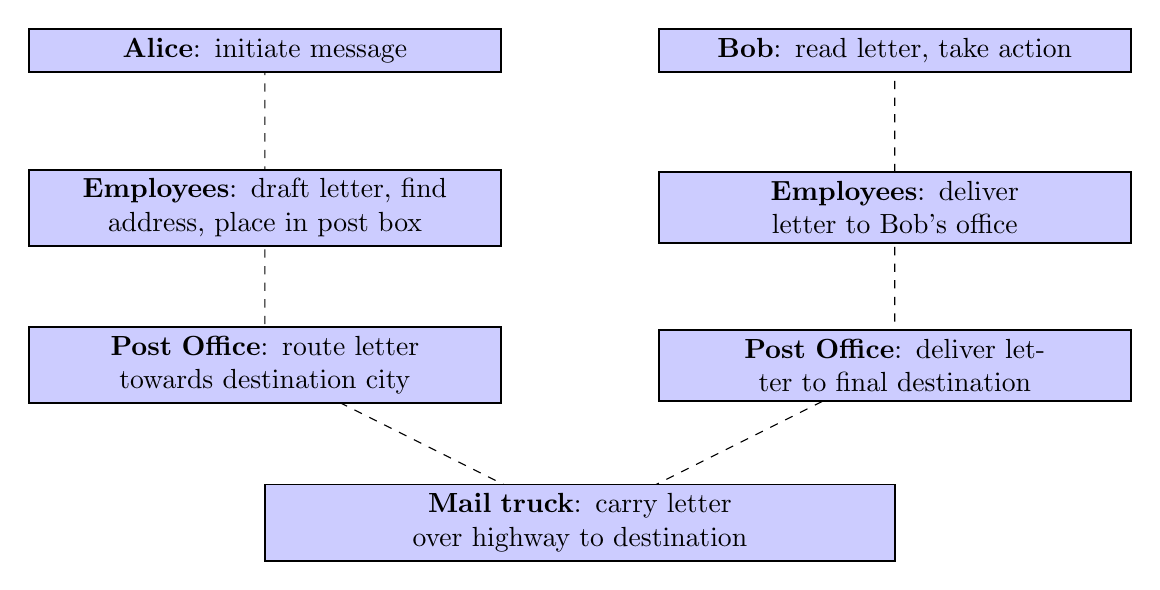
\begin{tikzpicture}[layer/.style={fill=blue!20,minimum width=6cm,align=center,text width=5.5cm,draw=black,solid,line width=.25mm}]
        \draw[dashed,-latex] (-4, 4) node[layer] {\textbf{Alice}: initiate message} --
        (-4, 2) node[layer] {\textbf{Employees}: draft letter, find address, place in post box} --
        (-4, 0) node[layer] {\textbf{Post Office}: route letter towards destination city} --
        (0, -2) node[layer,minimum width=8cm,text width=7.5cm] {\textbf{Mail truck}: carry letter over highway to destination} --
        (4, 0)  node[layer] {\textbf{Post Office}: deliver letter to final destination} --
        (4, 2)  node[layer] {\textbf{Employees}: deliver letter to Bob's office} --
        (4, 4)  node[layer] {\textbf{Bob}: read letter, take action};
    \end{tikzpicture}
    \caption{Layers of the postal system.}
    \label{fig:layer_mail}
\end{figure}

These layers all have counterparts in the Internet. At the top, we have the \emph{application layer}: programs which rely on the Internet and know how to initiate messages, much like Alice and Bob. The application layer relies on the \emph{transport layer} to determine an address where the messages should go, just as Alice relied on Jane to find Bob's mailing address. The transport layer relies on the \emph{Internet layer} to use the address to send the message to the right location, just as the Post Office routed Alice's letter to Bob's city. Finally, the transport layer relies on the \emph{link layer} to physically transmit data over wires or wireless protocols, just as the Post Office relies on mail trucks to move envelopes.

This set of four layers is commonly known as TCP/IP, named for the Transmission Control Protocol (TCP) which commonly runs the transport layer, and the Internet Protocol (IP) which commonly runs the Internet layer. The following sections contain more details on each of the layers and the protocols they use. You should always keep in mind that these layers work together just like the layers of the postal system work together.

\subsection{Application Layer}

The application layer is the highest layer of TCP/IP. It consists of various protocols that specify how to send different types of data over the Internet. You might have heard of one of these protocols, HTTP. HTTP stands for HyperText Transfer Protocol. It comes at the beginning of a web address. When you type \ic{http://www.google.com}, you're telling your computer to use HTTP to access \ic{www.google.com}.

There are many other protocols in the application layer. HTTPS is a secure version of HTTP, which uses security protocols we'll discuss in the next chapter. Another popular protocol is SSH, or Secure Shell, which programmers use to access the command line (see previous chapter) on another machine. The file transfer protocol, or FTP, is used for exchanging files between different computers. A variety of protocols, such as POP3, IMAP, and SMTP, are used for exchanging emails.

When the application layer receives data from the transport layer, it needs to know which protocol it was sent with. In order to sort out all the different data, the application layer uses \emph{ports}. All Internet communications happen over some numbered port. For example, HTTP uses port 80. When you load \ic{http://www.google.com}, your computer sends a request to Google over port 80, telling Google to load the home page. Google sends its home page back over port 80. Table \ref{tab:common_ports} lists the most commonly used protocols and the ports they use.

\begin{table}
    \centering
    \begin{tabular}{lll}
        Protocol & Port & Usage \\
        \hline
        HTTP & 80 & Web traffic \\
        HTTPS & 443 & Secure web traffic \\
        FTP & 21 & File transfer \\
        SSH & 22 & Remote shell access \\
        IMAP & 993 & Receiving email \\
        SMTP & 587 & Sending email
    \end{tabular}
    \caption{Commonly used Internet protocols.}
    \label{tab:common_ports}
\end{table}

If you write a program that uses the Internet, you will interact primarily with the application layer. A very common example is writing a program which runs on a web server. A web server is a computer which is connected to the Internet, and runs a program that constantly listens for incoming communications on ports 80 and 443 -- the ports used for the World Wide Web. When it receives a request, it will run a program and send the output of that program back to the requester. Every website is hosted by a web server, which knows how to send the data of the website to anyone who requests it.

A simple and famous example is \ic{isitfriday.net}. This website is hosted by a server which listens for requests. When it gets a request for \ic{isitfriday.net}, it will run a program which checks if it is Friday (you'll learn how to use ``if'' logic in programs in the next chapter). If it is Friday, it sends back a website that says ``Yes.'' Otherwise, it sends back a website that says ``Not yet.''

\subsection{Transport Layer}

When the application layer is ready to transmit a message, it will pass it down to the transport layer. By far the most common transport layer protocol is TCP, for Transmission Control Protocol. We will focus on TCP in this section. Another common protocol in the transport layer is TLS, for Transport Layer Security, which runs alongside TCP. We will discuss TLS more in the next chapter.

When TCP is asked to transfer a message, it will prepare to divide up the message and send it piece by piece over the network. The individual pieces are called \emph{packets}. These packets are relatively small, about a kilobyte. For reference, if you are sending an image over TCP, an average-sized image would typically be broken into a few thousand packets before being transferred. 

The reason for dividing up the message is that a major role of TCP is to guarantee reliability. 
%While the application layer assumes that its message will be sent in full and without errors, 
The Internet layer does not guarantee accurate or successful transmission, so it is the job of the transport layer to ensure robust communication. By breaking a message into small packets, TCP helps to reduce the chance that the entire message fails to transmit, since most of the packets will reach the destination. In addition, if a packet does fail to transmit, it doesn't take too much time to recover, since TCP can re-send the relatively small packet.

In addition to providing reliability, TCP is responsible for initiating connections between two computers. When TCP receives a request to transfer a message to a destination, it will first complete a ``handshake'' with that destination. The goal of the handshake is to establish that both parties are connected to the Internet and ready and willing to communicate with one another. In addition, the parties need to synchronize a \emph{sequence number} which specifies the numbers that will label subsequent packets.

We have already thought about handshakes between humans in some detail, so now let's delve into how TCP facilitates handshakes between computers. If humans were communicating using a TCP-style handshake, the conversation might look like this:
\begin{enumerate}
    \item Alice says to Bob, ``Let's start talking. I'll send some packets, starting with this one, \#3874.''
    \item Bob says to Alice, ``I hear you Alice, and I'm looking forward to packet \#3875. My packets will start with this one, \#8452.''
    \item Alice says to Bob, ``Great, I'm looking forward to packet \#8453.''
\end{enumerate}
This is the \emph{three-way handshake} model. First, Alice notifies Bob of her intent to communicate and synchronizes her sequence number. Then Bob sends an acknowledgement of Alice's sequence number, and also synchronizes his own sequence number. Finally, Alice acknowledge's Bob's sequence number, and then they are ready to communicate.

There are two kinds of messages being sent in the handshake, synchronization and acknowledgement. These are typically abbreviated as \ic{SYN} and \ic{ACK}. The TCP handshake protocol works as follows.
\begin{graybox}
{\Large TCP Handshake}
\begin{enumerate}
    \item $A$ generates a random number $x$. $A$ sends $\boxed{\ic{SYN}\ x}$ to $B$.
    \item $B$ generates a random number $y$. $B$ sends $\boxed{\ic{ACK}\ x+1}$ to $A$, and then sends $\boxed{\ic{SYN}\ y}$ to $A$.
    \item $A$ sends $\boxed{\ic{ACK}\ y+1}$ to $B$.
\end{enumerate}
\end{graybox}

\subsection{Internet Layer}

Perhaps the most interesting layer of the TCP/IP stack is the Internet layer, which almost always consists of the Internet Protocol (IP). This layer corresponds to the Post Office in our analogy: it is responsible for routing data where it needs to go. Just as the Post Office uses mailing addresses to specify locations, the Internet layer uses IP addresses to specify computers on the network.

An IP address is a sequence of 32 bits, grouped into blocks of 8. When they are written out, the groups of 8 bits are converted to decimal numbers between 0 and 255. The groups are separated by dots, so sometimes an IP address is referred to as a ``dotted quad.'' For example, the IP address \ic{172.217.15.78} points to the server which hosts \ic{www.google.com}. These addresses are stored in a sort of phone book called the Domain Name System, or DNS. When you type a website into your browser, it will first look up its IP address in the Domain Name System, and then request that IP address over the network.

When the Internet layer receives a packet from the transport layer for transmission, it will look at the IP address of the destination. It knows how to find a server which is closer to that destination. For example, if a server in New York City sees a packet destined for an IP address in Washington, DC., it might decide to forward that packet to a server in Philadelphia, PA.

You can view this process yourself using a Unix utility called \ic{traceroute}. Open a terminal and type \ic{traceroute} followed by any website. You'll see how the Internet Protocol routes your packets through different servers in order to reach their destination. For example, below is the route from a personal computer to \ic{youtube.com}. The address in the last line, \ic{172.217.12.238}, specifies the location of one of YouTube's servers.

\label{code:traceroute}
\begin{monospace}
# traceroute youtube.com
    1  192.168.1.1 (192.168.1.1)  0.448 ms  0.958 ms  0.966 ms
    2  * * *
    3  ae1312-21.ARTNVAFC-MSE01-AA-IE1.verizon-gni.net (100.41.21.152)  7.779 ms  7.766 ms  7.628 ms
    4  0.ae10.GW13.IAD8.ALTER.NET (140.222.225.219)  9.139 ms  9.117 ms  9.082 ms
    5  72.14.218.232 (72.14.218.232)  8.507 ms  7.277 ms  4.378 ms
    6  * * *
    7  216.239.54.106 (216.239.54.106)  4.779 ms 108.170.232.0 (108.170.232.0)  12.022 ms 108.170.246.33 (108.170.246.33)  16.086 ms
    8  108.170.246.67 (108.170.246.67)  12.976 ms 108.170.232.19 (108.170.232.19)  12.769 ms 108.170.246.66 (108.170.246.66)  10.935 ms
    9  iad30s15-in-f14.1e100.net (172.217.12.238)  10.570 ms 216.239.47.127 (216.239.47.127)  16.793 ms iad30s15-in-f14.1e100.net (172.217.12.238)  10.485 ms
\end{monospace}

The IP addresses we've described all correspond to version 4 of the Internet Protocol, or IPv4. There are about four billion unique IPv4 addresses, which seemed like plenty at the time of its creation. However, the growth of the Internet and the proliferation of mobile devices has led to the exhaustion of almost all IPv4 addresses. In order to ensure that the Internet can continue to grow, a transition to IPv6, which provides for many more addresses, is slowly taking place.

In the transport layer, we delved into the step-by-step procedure used for handshaking. These sorts of procedures are one important aspect of the protocols that run networks. Another important aspect is the format in which data is sent. The link layer, which we'll come to in the next section, can only send sequences of bits -- zeroes and ones -- so it is important for both parties to agree on which bits mean what.

To give an example of this, we will look inside the packets sent by IPv4. You should not try to memorize the following, but instead try to appreciate the importance of having a detailed packet structure.

An IP packet is divided into its \emph{header} and the \emph{data}. The header contains information about how the packet is being transmitted, while the data is the actual contents of the packet. The format of IPv4 headers is shown in Table \ref{tab:ipv4}. The various segments specify the following information.
\begin{itemize}
    \item \textbf{Version}: the first four bits specify the version of IP being used. For IPv4, these bits are always \ic{0100}, binary for 4.
    \item \textbf{IHL}: this is the Internet Header Length. This specifies the number of 32 bit blocks, called ``words,'' used by the header. In Table \ref{tab:ipv4} we show a header with 5 words, so these bits are \ic{0101}. This is almost always the case, although it is possible to have a larger IHL value and include additional data in the header.
    \item \textbf{DSCP}: this stands for Differentiated Services Code Point. These bits are used to specify the type of service for the packet. This allows the network to give priority to some packets, such as those used for voice or video calling, which need to arrive as quickly as possible.
    \item \textbf{ECN}: this stands for Explicit Congestion Notification. This allows the network to flag packets which are experiencing congestion along their routes.
    \item \textbf{Total Length}: this specifies the total length of the packet, in bytes including both the header and data. Since it is 16 bits, the maximum value is $2^{16}-1 = 65535$ bytes, or about 64 KB.
    \item \textbf{Fragmentation Data}: these bits are used to group packets which have been fragmented due to a maximum transmission size imposed by the link layer.
    \item \textbf{Time to Live}: this keeps track of how many hops a packet has made through the network. Every time the packet is forwarded along a new link in the network, this value is decreased by one. If it hits zero, the packet is dropped and the sender is notified. This is how the \ic{traceroute} utility works: it sends packets with small Time to Live values, and waits for the notifications to see where the packet was after one hop, two hops, etc.
    \item \textbf{Protocol}: this specifies the transport layer protocol which is making use of IP. For example, for TCP the protocol value is set to 6.
    \item \textbf{Header Checksum}: these bits are used for correcting errors in the header. The idea of a ``checksum'' is encoded in the word: we could imagine transmitting a stream of bits, followed by a few bits that count the number of ones in the original stream. If a zero was flipped to a one, or a one was flipped to a zero, then the receiver will notice that the checksum does not match and can ask for the packet to be resent. In practice a checksum is a more complicated function of the bits, but the idea is the same.
    \item \textbf{Source IP Address}: this is the address of the device sending the packet. Note that it spans 32 bits, since an IPv4 address consists of four numbers each from 0 -- 255, which require 8 bits each.
    \item \textbf{Destination IP Address}: this is the address of the device meant to receive the packet.
\end{itemize}

\begingroup
\tabcolsep=0.05cm
\begin{table}
    \centering
    \footnotesize
    \begin{tabular}{|c|c|c|c|c|c|c|c|c|c|c|c|c|c|c|c|c|c|c|c|c|c|c|c|c|c|c|c|c|c|c|c|c|}
        \hline
        Bit & 0 & 1 & 2 & 3 & 4 & 5 & 6 & 7 & 8 & 9 & 10 & 11 & 12 & 13 & 14 & 15 & 16 & 17 & 18 & 19 & 20 & 21 & 22 & 23 & 24 & 25 & 26 & 27 & 28 & 29 & 30 & 31 \\
        \hline
        0 & \multicolumn{4}{c|}{Version} & \multicolumn{4}{c|}{IHL} & \multicolumn{6}{c|}{DSCP} & \multicolumn{2}{c|}{ECN} & \multicolumn{16}{c|}{Total Length} \\
        \hline
        32 & \multicolumn{32}{c|}{Fragmentation Data} \\
        \hline
        64 & \multicolumn{8}{c|}{Time to Live} & \multicolumn{8}{c|}{Protocol} & \multicolumn{16}{c|}{Header Checksum} \\
        \hline
        96 & \multicolumn{32}{c|}{Source IP Address} \\
        \hline
        128 & \multicolumn{32}{c|}{Destination IP Address} \\
        \hline
    \end{tabular}
    \caption{The IPv4 header format.}
    \label{tab:ipv4}
\end{table}
\endgroup

\subsection{Link Layer}

Finally, we come to the actual nuts and bolts of the Internet: how are individual pieces of data sent across the network? This part of networking is handled by the link layer.

There are two main link layer technologies you will encounter. The first is Ethernet, which is used for wired Internet connections. An Ethernet cable, also known as an RJ-45 cable, is shown in Figure \ref{fig:ethernet}. Each end of the cable has an 8-pin connector. Inside the cable, a twisted pair of wires can carry signals in both directions without having them collide with each other.

\begin{figure}
    \centering
    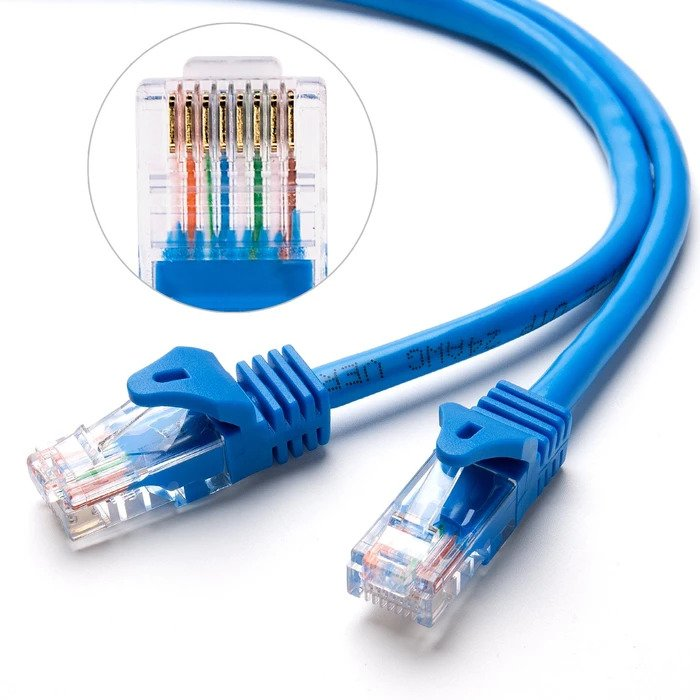
\includegraphics[width=.6\linewidth]{images/ethernet.jpg}
    \caption{An Ethernet cable used to network computers together.}
    \label{fig:ethernet}
\end{figure}

The other primary link layer technology is 802.11, more commonly known as Wi-Fi. With a wired network, signals can be sorted into separate wires so they don't overlap, but over a wireless network signals are broadcast and have the potential to interfere with one another. In order to prevent this, Wi-Fi is designed to allow devices to operate at slightly different frequencies which are arranged into channels.

There are two major variants of Wi-Fi: 2.4 gigahertz (GHz) and 5 GHz. These are two different frequency bands. Within each of them there are multiple channels. At 2.4 GHz, which was the first frequency available for Wi-Fi, there are 11 channels. However, the channels overlap with one another, so it is best for devices to use channels 1, 6, and 11, reducing the efffective number of channels down to 3. The newer 5 GHz protocol alleviates this problem by making hundreds of channels available. Most new devices can operate at either 2.4 GHz or 5 GHz, but some older devices only support 2.4 GHz.

The details of link layer technologies are complex, but luckily you rarely have to deal with them directly. In most cases, Ethernet or Wi-Fi have been engineered to the point where little effort is required to make them work properly, and you can focus on other layers of the network while trusting that signals are being carried appropriately by the link layer.

\exercisesection

\begin{exercise}
    Put the following layers in order from top to bottom, and give an example of a protocol or technology used in each layer.
    \begin{itemize}
        \item Transport Layer
        \item Link Layer
        \item Application Layer
        \item Internet Layer
    \end{itemize}
\end{exercise}

% this seems way too hard

%\begin{exercise}
%    Identify all of the following blocks of IP addresses which contain 48.192.72.86. (\emph{Hint:} you may want to write out each address block in binary.)
%    \begin{itemize}
%        \item 48.192.0.0/12
%        \item 48.192.0.0/16
%        \item 48.192.0.0/20
%        \item 48.0.0.0/4
%        \item 48.0.0.0/8
%        \item 48.0.0.0/12
%        \item 48.192.64.0/20
%        \item 48.192.64.0/24
%    \end{itemize}
%\end{exercise}

\begin{exercise}
    In a TCP handshake, Alice initiates by sending $\boxed{\ic{SYN}\ 895}$ to Bob. Give an example of the remaining steps that could take place in this handshake.
\end{exercise}

\begin{exercise}
    What is the main advantage of 5 GHz WiFi over 2.4 GHz WiFi? Why is 2.4 GHz WiFi still in use?
\end{exercise}
	
	%SEMESTER BREAK (there be dragons here)
	
	\chapter{Arrays}
\label{ch:arrays}

\begin{goals}
\item 
\end{goals}

Arrays are used to store multiple values in a single variable, instead of declaring separate variables for each value.

To declare an array, define the variable type with square brackets:

\begin{code}
String[] cars;
\end{code}

We have now declared a variable that holds an array of strings. To insert values to it, we can use an array literal - place the values in a comma-separated list, inside curly braces:

\begin{code}
String[] cars = {"Volvo", "BMW", "Ford", "Mazda"};
\end{code}

To create an array of integers, you could write:

\begin{code}
int[] myNum = {10, 20, 30, 40};
\end{code}

You access an array element by referring to the index number. This statement accesses the value of the first element in cars:
\begin{code}
String[] cars = {"Volvo", "BMW", "Ford", "Mazda"};
System.out.println(cars[0]);
// Outputs Volvo
\end{code}

Note that in Java (and many other programming languages) the first array element is 0 rather than 1! This is a bit unintuitive, and the source of many coding bugs. 

\begin{figure}
	\centering
	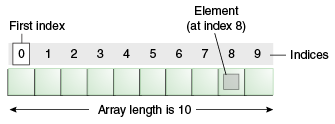
\includegraphics[width=0.5\textwidth]{images/array-diagram.png}
	\caption{Diagram of an array (Credit: https://www.geeksforgeeks.org/arrays-in-java/)}
\end{figure}

To change the value of a specific element, refer to the index number:

\begin{code}
String[] cars = {"Volvo", "BMW", "Ford", "Mazda"};
cars[0] = "Opel";
System.out.println(cars[0]);
// Now outputs Opel instead of Volvo
\end{code}

To find out how many elements an array has, use the length property:

\begin{code}
String[] cars = {"Volvo", "BMW", "Ford", "Mazda"};
System.out.println(cars.length);
// Outputs 4
\end{code}

You can loop through the array elements with the for loop, and use the length property to specify how many times the loop should run.

The following example outputs all elements in the cars array:

\begin{code}
String[] cars = {"Volvo", "BMW", "Ford", "Mazda"};
for (int i = 0; i < cars.length; i++) {
  System.out.println(cars[i]);
}
\end{code}

\begin{example}Where is the bug?
\begin{code}
int[] arr = new int[100]; 
for (int i = 0; i <= 100; ++i) {
    System.out.println(arr[i]);
}
\end{code}
\noindent \emph{Answer}:
The issue is that the program attempts to access the value \ic{arr[100]}, while the last element in the array is \ic{arr[99]}.

This kind of bug is called an ``off-by-one error'' and is so common it has a name. In general, an off-by-one-error is one in which a loop iterates one time too many or too few.

\end{example}

Sometimes it is also useful to initialize the array in a for loop rather than typing in the values by hand. For example, suppose you wanted an array full of the integers from 0 to 999. This would be very hard to type! To complete this task, we could instead use the following code snippet:

\begin{code}
int n = 1000;
int[] numbersArray = new int[n];
for (int i=0; i<n; i++) {
  numbersArray[i]=i;
}
\end{code}

In this code, we initialize an array then use a for loop to fill it, rather than typing in the values ourselves. Just like when we worked with Scanners, the ``new" keyword is needed to initialize an empty array so that we can loop over it. The size must be set from the beginning (and can't be changed after!) within brackets []. In this case, we are initializing an integer array of size 1000 (i.e. \ic{n}). 

\begin{example}
What are the values of the integer array \ic{arr} by the end of this code snippet? 
\begin{code}
    int n=6;
    
    int[] arr = new int[n];
    for (int i=0; i<n; i++) {
      arr[i]=i;
    }

    for (int i = 0; i < arr.length/2; i++) {
      int tmp = arr[i];
      arr[i] = arr[arr.length-1-i];
      arr[arr.length-i-1] = tmp;
    }
\end{code}

\noindent \emph{Answer}:
\ic{arr} is initialized to be the integers from 0 through 5. The second block loops over the first 3 array values and swaps the 0 index value with the 5, the 1 with the 4, and the 2 with the 3. By the end, the array has been reversed.

\end{example}

\marginnote{This array-reversal example is extremely hard if you think about it in the abstract. But it's not as bad when you write out the array on paper and make the changes from the for loop as you go, carefully writing down every change. Even great developers use paper and pencil to write and debug code, especially for loops and arrays!}

% There is also a "for-each" loop, which is used exclusively to loop through elements in arrays:

% \begin{code}
% for (type variable : arrayname) {
%   ...
% }
% \end{code}

% The following example outputs all elements in the cars array, using a "for-each" loop:

% \begin{code}
% String[] cars = {"Volvo", "BMW", "Ford", "Mazda"};
% for (String i : cars) {
%   System.out.println(i);
% }
% \end{code}

% The example above can be read like this: for each String element (called i - as in index) in cars, print out the value of i.

% If you compare the for loop and for-each loop, you will see that the for-each method is easier to write, it does not require a counter (using the length property), and it is more readable.

A multidimensional array is an array containing one or more arrays.

To create a two-dimensional array, add each array within its own set of curly braces:

\begin{code}
int[][] myNumbers = { {1, 2, 3, 4}, {5, 6, 7} };
\end{code}

myNumbers is now an array with two arrays as its elements.

To access the elements of the myNumbers array, specify two indexes: one for the array, and one for the element inside that array. This example accesses the third element (2) in the second array (1) of myNumbers:

\begin{code}
int[][] myNumbers = { {1, 2, 3, 4}, {5, 6, 7} };
int x = myNumbers[1][2];
System.out.println(x); // Outputs 7
\end{code}

We can also use a for loop inside another for loop to get the elements of a two-dimensional array (we still have to point to the two indexes):

\begin{code}
public class MyClass {
  public static void main(String[] args) {
    int[][] myNumbers = { {1, 2, 3, 4}, {5, 6, 7} };
    for (int i = 0; i < myNumbers.length; ++i) {
      for(int j = 0; j < myNumbers[i].length; ++j) {
        System.out.println(myNumbers[i][j]);
      }
    }
  }
}
\end{code}



% Consider this snippet of code:

% \begin{code}
% if      (day ==  0) System.out.println("Monday");
% else if (day ==  1) System.out.println("Tuesday");
% else if (day ==  2) System.out.println("Wednesday");
% else if (day ==  3) System.out.println("Thursday");
% else if (day ==  4) System.out.println("Friday");
% else if (day ==  5) System.out.println("Saturday");
% else if (day ==  6) System.out.println("Sunday");
% \end{code}

% \noindent What does this code do? It prints the day of the week after conditioning on the value of an integer \ic{day}. But this code is repetitive. It would be useful if we had some way of creating a list of days of the week, and then just specifying which of those days we wanted to print. Something like this:

% \begin{code}
% System.out.println(DAYS\_OF\_WEEK[day]);
% \end{code}

% To achieve this in Java, we need arrays.

% \begin{definition}
% An \emph{array} is a fixed-length list of values that are of the same type. We can access data in an array by \emph{indexing}, which means referring to specific values in the array by number. If an array has \ic{n} values, then we think of it as being numbered from \ic{0} to \ic{n-1}.
% \end{definition}

% \begin{figure}
% 	\centering
% 	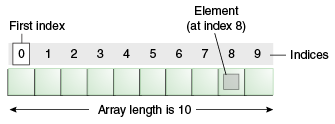
\includegraphics[width=0.5\textwidth]{images/array-diagram.png}
% 	\caption{Diagram of an array (Credit: https://www.geeksforgeeks.org/arrays-in-java/)}
% \end{figure}

% To \emph{loop} or \emph{iterate} over an array means that our program accesses every value in the array, typically in order. For example, if we looped over the array in the diagram, that would mean that we looked at the value at the 0th index, then the value at the 1st index, then the value at the 2nd index, and so on.

% Arrays are \emph{fixed-length}, meaning that after we have created an array, we cannot change its length. We will see next semester that \ic{ArrayLists} are an array-like data structure that allows for changing lengths.

% Finally, all the values in an array must be of the same type. For example, an array can hold all floating point numbers or all characters or all strings. But an array cannot hold values of different types.

% \section{Creating arrays}

% The syntax for creating an array in Java has three parts:

% \begin{enumerate}
% \item Array type
% \item Array name
% \item Either: array size or specific values
% \end{enumerate}

% For example, this code creates an array of size \ic{n = 10} and fills it with all \ic{0.0}s

% \begin{code}
% double[] arr;                    // Declare array
% arr = new double[n];             // Initialize the array
% for (int i = 0; i < n; i++) {    // Iterate over array
%     arr[i] = 0.0;                // Initialize elements to 0.0
% }
% \end{code}

% The key steps are: we first declare and initialize the array. We then loop over the array to initialize specific values. We can also initialize the array at compile time, for example

% \begin{code}
% String[] DAYS_OF_WEEK = {
% //  Indices:
% //  0      1      2      3      4      5      6
%     "Mon", "Tue", "Wed", "Thu", "Fri", "Sat", "Sun"
% };
% \end{code}

% Notice the difference in syntax. When creating an empty array, we must specify a size. When initialize an array at compile time with specific values, the size is implicit in the number of values provided.

% Finally, in Java, it is acceptable to move the brackets to directly after the type declaration to directly after the name declaration. For example, these two declarations are equivalent:

% \begin{code}
% int arr[];
% int[] arr;
% \end{code}

% \section{Indexing}

% Consider the array \ic{DAYS\_OF\_WEEK} from the previous section. We can \emph{index} the array using the following syntax:

% \begin{code}
% System.out.println(DAYS_OF_WEEK[3]);  // Prints "Thu"
% \end{code}

% In Java, array's are said to use \emph{zero-based indexing} because the first element in the array is accessed with the number \ic{0} rather than \ic{1}.

% \begin{example}
% What does \ic{System.out.println(DAYS\_OF\_WEEK[1]);} print?
% \end{example}

% \begin{example}
% What does this code do? What number does it print?

% \begin{code}
% double sum = 0.0;
% double[] arr = { 1, 2, 2, 3, 4, 7, 9 }
% for (int i = 0; i < arr.length; i++) {
%     sum += arr[i];
% }
% System.out.println(sum / arr.length);
% \end{code}
% \end{example}

% \section{Array length}

% As mentioned previously, arrays are \emph{fixed-length}. After you have created an array, it's length is unchangeable. You can access the length of an array \ic{arr[]} with the code \ic{arr.length}.

% \begin{example}
% What does \ic{System.out.println(DAYS\_OF\_WEEK.length);} print?
% \end{example}

% \begin{example}
% Write a \ic{for} loop to print the days of the week in order (Monday through Sunday) using an array rather than seven \ic{System.out.println} function calls.
% \end{example}

% \section{Default initialization}

% In Java, the default initial values for numeric primitive types is \ic{0} and \ic{false} for the \ic{boolean} type.

% \begin{example}
% Consider this code from earlier:

% \begin{code}
% double[] arr;
% arr = new double[n];
% for (int i = 0; i < n; i++) {
%     arr[i] = 0.0;
% }
% \end{code}

% Rewrite this code to be a single line.
% \end{example}

% \section{Bounds checking}

% Consider this snippet of code.

% \begin{example}Where is the bug?
% \begin{code}
% int[] arr = new int[100]; 
% for (int i = 0; i <= 100; ++i) {
%     System.out.println(arr[i]);
% }
% \end{code}
% \end{example}

% The issue is that the program attempts to access the value \ic{arr[100]}, while the last element in the array is \ic{arr[99]}.

% This kind of bug is called an ``off-by-one error'' and is so common it has a name. In general, an off-by-one-error is one in which a loop iterates one time too many or too few.

% \begin{example}
% Where is the off-by-one-error?

% \begin{code}
% int[] arr = new int[100];
% for (int i = 0; i < array.length; i++) {
%     arr[i] = i;
% }
% for (int i = 100; i > 0; --i) {
%     System.out.println(arr[i]);
% }
% \end{code}
% \end{example}

% \begin{example}
% Fill in the missing code in this \ic{for} loop to print the numbers in reverse order, i.e. \ic{5, 4, 3, 2, 1}:

% \begin{code}
% int[] arr = { 1, 2, 3, 4, 5 };
% for (???) {
%     System.out.println(arr[i]);
% }
% \end{code}
% \end{example}

% \section{Empty arrays}

% This code prints five values, one per line, but we never specified which values. What do you think it prints?

% \begin{code}
% int[] arr = new int[5];
% for (int i = 0; i < arr.length; i++) {
%     System.out.println(arr[i]);
% }
% \end{code}

% In Java, an unitialized or empty array is given a default value:

% \begin{itemize}
% \item For \ic{int}, \ic{short}, \ic{byte}, or \ic{long}, the default value is \ic{0}.
% \item For \ic{float} or \ic{double}, the default value is \ic{0.0}
% \item For \ic{boolean} values, the default value is \ic{false}.
% \item For \ic{char}, the default value is the null character \ic{'\u0000'}.
% \end{itemize}

% Note that an array can be partially initialized.

% \begin{example}
% What does this code print?

% \begin{code}
% char[] alphabet = new char[26];
% alphabet[0] = 'a';
% alphabet[1] = 'b';
% for (int i = 0; i < alphabet.length; i++) {
%     System.out.println(alphabet[i]);
% }
% \end{code}
% \end{example}

% \section{Enhanced for loop}

% So far, we have seen how to iterate over arrays by indexing each element with a number:

% \begin{code}
% char[] vowels = {'a', 'e', 'i', 'o', 'u'};
% for (int i = 0; i < vowels.length; ++ i) {
%     System.out.println(vowels[i]);
% }
% \end{code}

% We can perform the same iteration without using indices using an ``enhanced \ic{for} loop'' or \ic{for-each} loops:

% \begin{code}
% char[] vowels = {'a', 'e', 'i', 'o', 'u'};
% for (char item: vowels) {
%     System.out.println(item);
% }
% \end{code}

% \section{Exchanging and shuffling}

% Two common tasks when manipulating arrays are \emph{exchanging two values} and \emph{shuffling} values. (\emph{Sorting} is more complicated and will be address later.)

% To exchange to values, consider the following code:

% \begin{code}
% double[] arr = { 1.0, 2.0, 3.0, 4.0, 5.0, 6.0 };
% int i = 1;
% int j = 4;
% double tmp = arr[i]; 
% arr[i] = arr[j]; 
% arr[j] = tmp;
% \end{code}

% \begin{example}
% What are the six values in the array, in order?
% \end{example}

% To shuffle the array, consider the following code:

% \begin{code}
% int n = arr.length; 
% for (int i = 0; i < n; i++) { 
%     int r = i + (int) (Math.random() * (n-i)); 
%     String tmp = arr[r];
%     arr[r] = arr[i];
%     arr[i] = tmp;
% }
% \end{code}

% \begin{example}
% What does this code do?

% \begin{code}
% for (int i = 0; i < n/2; i++) {
%     double tmp = arr[i];
%     arr[i] = arr[n-1-i];
%     arr[n-i-1] = tmp;
% }
% \end{code}
% \end{example}

% \exercisesection

% \begin{exercise}
% Write a program that reverses the order of values in an array.
% \end{exercise}

% \begin{exercise}
% What is wrong with this code snippet?

% \begin{code}
% int[] arr;
% for (int i = 0; i < 10; i++) {
%     arr[i] = i;
% }
% \end{code}
% \end{exercise}

% \begin{exercise}
% Rewrite this snippet using an enhanced \ic{for-each} loop (for now, it is okay to re-define the array):

% \begin{code}
% char[] vowels = {'a', 'e', 'i', 'o', 'u'};
% for (int i = array.length; i >= 0; i--) {
%     char letter = vowels[i];
%     System.out.println(letter);
% }
% \end{code}
% \end{exercise}

% \begin{exercise}
% Write a program that uses \ic{for} loops to print the following pattern:

% \begin{code}
% 1********

% 12*******

% 123******

% 1234*****

% 12345****

% 123456***

% 1234567**

% 12345678*

% 123456789
% \end{code}
% \end{exercise}

% \begin{exercise}
% Write a program \ic{HowMany.java} that takes an arbitrary number of command line arguments and prints how many there are.
% \end{exercise}

% \referencessection

% Computer Science: An Interdisciplinary Approach, Robert Sedgewick and Kevin Wayne.

	
	\chapter{ArrayLists}

A \emph{collection} is a group of objects. Today, we'll be looking at a very useful collection, the \ic{ArrayList}. A \emph{list} is an ordered collection, and an \ic{ArrayList} is one type of list. We will see at the end of this chapter how an \ic{ArrayList} is different from an \ic{array}.

\section{Creating an \ic{ArrayList}}

Let's create a class \ic{NameTracker} and follow along in it. Before we can use an ArrayList, we have to import it:

\begin{code}
import java.util.ArrayList;

public class NameTracker {
    
    public static void main(String args[]) {
    }
}
\end{code}

\noindent Next, we call the constructor; but we have to declare the type of object the \ic{ArrayList} is going to hold. This is how you create a new \ic{ArrayList} holding \ic{String} objects.

\begin{code}
ArrayList<String> names = new ArrayList<String>();
\end{code}

\noindent Notice the word ``String'' in angle brackets. This is the Java syntax for constructing an ArrayList of String objects.

\section{\ic{add()}}

We can add a new String to names using the \ic{add()} method.

\begin{code}
names.add("Ana");
\end{code}

\begin{example}
Exercise: Write a program that asks the user for some names and then stores them in an ArrayList. Here is an example program:

\begin{monospace}
Please give me some names:
Sam
Alecia
Trey
Enrique
Dave

Your name(s) are saved!
\end{monospace}
\end{example}

\noindent We can see how many objects are in our ArrayList using the size() method.

\begin{code}
System.out.println(names.size()); // 5
\end{code}

\begin{example}
Modify your program to notify the user how many words they have added.

\begin{monospace}
Please give me some names:
Mary
Judah

Your 2 name(s) are saved!
\end{monospace}
\end{example}

\section{\ic{get()}}

Remember how the \ic{String.charAt()} method returns the \ic{char} at a particular index? We can do the same with names. Just call \ic{get()}:

\begin{code}
names.add("Noah");
names.add("Jeremiah");
names.add("Ezekiel");
System.out.println(names.get(2)); // ``Ezekiel''
\end{code}

\begin{example}
Update your program to repeat the names back to the user in reverse order. Your solution should use a for loop and the size() method. For example:

\begin{monospace}
Please give me some names:
Ying
Jordan

Your 2 name(s) are saved! They are:
Jordan
Ying
\end{monospace}
\end{example}

\section{\ic{contains()}}

Finally, we can ask our names \ic{ArrayList} whether or not it has a particular string.

\begin{code}
names.add("Veer");
System.out.println(names.contains("Veer")); // true
\end{code}

\begin{example}
Update your program to check if a name was input by the user. For example:

\begin{monospace}
Please give me some names:
Ying
Jordan

Search for a name:
Ying

Yes!
\end{monospace}
\end{example}

\section{\ic{ArrayList}s with custom classes}

An \ic{ArrayList} can hold any type of object! For example, here is a constructor for an \ic{ArrayList} holding an instance of a \ic{Person} class:

\begin{code}
ArrayList<Person> people = new ArrayList<Person>();
\end{code}

\noindent where \ic{Person} is defined as

\begin{code}
public class Person {

    String name;
    int age;

    public Person(String name, int age) {
        this.name = name;
        this.age = age;
    }

    public String getName() {
        return this.name;
    }

    public int getAge() {
        return this.age;
    }
}
\end{code}

\begin{example}
Modify our program to save the user's input names as Person instances. Rather than storing String objects in the ArrayList, store Person objects by constructing them with the input name. You'll need to use the Person constructor to get a Person instance!
\end{example}

\section{\ic{Arrays} versus \ic{ArrayLists}}

The most important difference between an array and an \ic{ArrayLists} is that an \ic{ArrayLists} is dynamically resized. Notice that when we created an \ic{ArrayLists}, we did not specify a size. But when we create an array, we must:

\begin{code}
int[] numbers1 = new int[10];
ArrayList<Integer> numbers2 = new ArrayList<Integer>();
\end{code}

In the first line of code, we create an array of length 10, and we cannot add more than 10 elements to \ic{numbers1}. In the second line of code, we create an \ic{ArrayList}, but we do not need to specify a size.

The second distinction between arrays and \ic{ArrayLists} is syntax. In Java, nearly everything is a class. An \ic{ArrayList} is a class with useful methods such as \ic{get()} and \ic{contains()} and is therefore more ``Java-like''. Arrays are not quite primitives such as \ic{ints} and note quite classes. Most likely, their syntax was borrowed from the C or C++ programming languages.

\exercisesection

\begin{exercise} Write a class BlueBook that tells the user the price of their car, depending on the make, model, and year. You should use Car.java and the stencil file provided, BlueBook.java. Your program depends on what cars your BlueBook supports, but here is an example program:

\begin{monospace}
What is your car's make?
Toyota
What is your Toyota's model?
Corolla
What is your Toyota Corolla's year?
1999

Your 1999 Toyota Corolla is worth \$2000.
\end{monospace}

\end{exercise}

\begin{exercise}
Notify the user if the car is not in your BlueBook.
\end{exercise}

\begin{exercise}
Clean up main by putting your code for creating the ArrayList in a separate method. What type should the method return?
\end{exercise}

\begin{exercise}
If the car is not in the BlueBook, ask the user to input the relevant data, construct a new Car instance, add it to your ArrayList.
\end{exercise}

\referencessection

1. \url{https://github.com/accesscode-2-1/unit-0/blob/master/lessons/week-3/2015-03-24_arraylists.md}
	
	\chapter{Classes}
\label{ch:classes}

Java is an \emph{object-oriented programming} (OOP) language, meaning that nearly everything is a ``class'' or an ``object''. While you may not have thought about it, you have been working with classes and objects this whole time. Now let's define these terms:

\begin{definition}
An \emph{object} is a combination of variables, functions, and data (state and behavior).
\end{definition}

\begin{definition}
A \emph{class} is a blueprint for a type of object.
\end{definition}

For example, if a car is an object, then a class is a car factory. Every car (object) that is made by the car factory (class) follows the basic car blueprint: it has tires, an engine, a steering wheel, and so forth. The type of an object is its class. So the type of an object from a car factory might be \ic{Car}.

As another example, here is a class that is very similar to classes you saw in Chapter~\ref{ch:methods}:

\begin{code}
/* HelloWorld.java */

class HelloWorld {

    static void greeting() {
        System.out.println("Hello World");
    } 

    public static void main(String[] args) {
        greeting();
    }
}
\end{code}

Every program in Java follows this basic pattern. You have a class, for example \ic{HelloWorld}. The name of the file must match the name of the class, for example \ic{HelloWorld.java}. Methods such as \ic{greeting} are associated with the class. And every Java program needs one \ic{main} method that gets executed first. In this chapter, we'll discuss classes in more detail. This will allow us to build more complex and interesting programs.

\section{Creating objects}

We've been working with classes this whole time. And in fact, you've also already seen objects. Consider this program from Chapter~\ref{ch:io}:

\begin{code}
import java.util.Scanner;

class HelloPlanet {

    public static void main(String[] args) {
        // Create a Scanner object.
        Scanner input = new Scanner(System.in);
        System.out.println("Enter a planet name: ");
        String planet = input.next();
        System.out.printf("Hello %s\n", planet);
        input.close();  // Close the Scanner object.
    }
}
\end{code}

Notice that on Line 7, we create an object \ic{input} using the \ic{new} keyword. We say that \ic{input} has type \ic{Scanner}. Again, nearly everything in Java is an object, so a similar thing is happening on line 9: \ic{String planet = ...} is creating a \ic{planet} object of type \ic{String}. This object is the user's input, e.g. "Jupiter".

Since a class is like a factory for objects of a given type, this means we can create multiple objects from a single class. Consider this example of two objects of type \ic{Dog}:

\begin{code}
class Dog {

    void bark() {
        System.out.println("Woof, woof!");
    }
    
    public static void main(String[] args) {
        Dog fido = new Dog();
        fido.bark();  // Prints "Woof, woof!"
        Dog izzy = new Dog();
        izzy.bark();  // Prints "Woof, woof!"
        // False; they are not the same object.
        System.out.println(fido == izzy);
    }
}
\end{code}

The important point is that \ic{fido} and \ic{izzy} are both \ic{Dog} objects. They both have a \ic{bark} method. But they're distinct objects.

\section{Class methods and attributes}

We have seen that classes have methods. For example, this snippet calls the \ic{Scanner} class's \ic{nextInt} method:

\begin{code}
Scanner input = new Scanner(System.in);
int num = input.nextInt();
\end{code}

However, classes also have \emph{attributes}. An attribute, sometimes called a \emph{field}, is a variable associated with a class. Every object constructed from the class will then have the same variable name, although not necessarily the same value. For example, we can modify the \ic{Dog} class to have a \ic{color} attribute:

\begin{code}
class Dog {

    // Un-initialized `color` attribute.
    String color;

    void bark() {
        System.out.println("Woof, woof!");
    }
    
    public static void main(String[] args) {
        Dog fido = new Dog();
        fido.color = "brown";
        Dog izzy = new Dog();
        izzy.color = "black";
        System.out.println(fido.color);  // Prints "brown"
        System.out.println(izzy.color);  // Prints "black"
    }
}
\end{code}

Notice that we access the attributes like we access methods, using dot notation. So while both \ic{Dog} objects have an \ic{age} attribute, that attribute is different for each instance. Setting Fido's color does not effect Izzy's color, although both dogs have colors.

Furthermore, a method can depend on the value of an attribute. Therefore, the runtime behavior of an object may depend on the object's state. For example

\begin{code}
class Dog {

    int age = 0;
    
    void bark() {
        System.out.printf("Woof! I'm %d-years-old.\n", age);
    }
    
    public static void main(String[] args) {
        Dog fido = new Dog();
        fido.age = 3;
        Dog izzy = new Dog();
        izzy.age = 5;
        fido.bark();  // Prints "Woof! I'm 3-years-old."
        izzy.bark();  // Prints "Woof! I'm 5-years-old."
    }
}
\end{code}

Notice that the result of calling the method \ic{bark} can change depending on the object's state.  This is what we mean when we say, ``Java is an object-oriented programming language.'' Nearly everything in Java is actually a class or an object, and we build complex programs by composing objects and by manipulating them and their states.

\section{Constructors}

We may want to set attributes such as Izzy's age when we create the object. We can do this using a constructor. In Java, a \emph{constructor} is a special method that initializes the object. The constructor is called when the class is created. For example:

\begin{code}
class Dog {

    // Declare but do not initialize class attributes.
    String color;
    int age;
    
    // This is a class constructor for the `Dog` class.
    public Dog(String myColor, int myAge) {
        color = myColor;
        age = myAge;
    }
    
    void bark() {
        System.out.printf("Woof! I have %s fur and %d-years-old.\n", age);
    }
    
    public static void main(String[] args) {
        Dog fido = new Dog("brown", 3);
        Dog izzy = new Dog("black", 5);
        // Prints "Woof! I have brown fur and 3-years-old."
        fido.bark();
        // Prints "Woof! I have black fur and 5-years-old."
        izzy.bark();
    }
}
\end{code}

As we can see, the \ic{Dog} constructor is a bit like a method in that it can accept parameters, in this case \ic{myColor} and \ic{myAge}. However, it is only called once per object using the \ic{new} keyword.

\section{Creating multiple classes}

Since every Java class must go into a separate file, we can create programs with multiple classes by creating separate files with their respective class definitions and then compiling those files together.

Let's look at an example. Consider these two classes, \ic{Car} and \ic{CarDealership}:

\begin{code}
// Car.java

class Car {
  
  String make;
  double price;
 
  public Car(String myMake, double myPrice) {
    make = myMake;
    price = myPrice;
  }
}
\end{code}

\begin{code}
// CarDealership.java

class CarDealership {
  
  public static void printPrice(Car car) {
    System.out.printf("%s costs: $%1.2f\n", car.make, car.price);
  }
    
  public static void main(String[] args) {
    Car car1 = new Car("Toyota", 12000);
    Car car2 = new Car("Ford", 8000);
    printPrice(car1);
    printPrice(car2);
  }
}
\end{code}

The \ic{Car} class represent car objects. Its constructor takes a string, for the car's make or brand name, such as Lincoln, Ford, and Chevrolet, as well a price. The \ic{CarDealership} class uses the \ic{Car} class to print information about each car. 
We can compile these two files together by passing both filenames to the \ic{javac} command:

\begin{monospace}
$ javac Car.java CarDealership.java
\end{monospace}

Notice that between these two files, there is only one \ic{main} method. This represents the start of the program. If we try to run the compiled \ic{Car} program, we will get an error:

\begin{monospace}
$ java Car
Error: Main method not found in class Car, please define the main method as:
   public static void main(String[] args)
or a JavaFX application class must extend javafx.application.Application
\end{monospace}

This error tells us that the \ic{java} executable cannot find the \ic{main} method to start the program. Instead, we need to run the \ic{CarDealership} program:

\begin{monospace}
$ java CarDealership
Toyota costs: $12000.00
Ford costs: $8000.00
\end{monospace}

We can imagine more complex programs. For example, here is a program that computes the average price of the cars in the dealership:

\begin{code}
import java.util.ArrayList;

class CarDealership {
  
  public static void printAveragePrice(ArrayList<Car> cars) {
    double avg = 0;
    for (Car car : cars ) {
      avg += car.price;
    }
    avg = avg / cars.size();
    System.out.printf("Average price: %1.2f\n", avg);
  }
    
  public static void main(String[] args) {
    ArrayList<Car> cars = new ArrayList<Car>();
    cars.add(new Car("Toyota", 12000));
    cars.add(new Car("Ford", 8000));
    cars.add(new Car("Lincoln", 13500));
    printAveragePrice(cars);
  }
}
\end{code}

After compiling this program and running it, we get

\begin{monospace}
$ java CarDealership
Average price: 11166.67
\end{monospace}

Now that we understand methods, arrays and \ic{ArrayLists}, and multiple class programs, we can really start to build cool stuff.

\section{Encapsulation}

Now that we can build programs with multiple classes, we need to talk about a concept called ``encapsulation'':

\begin{definition}
\emph{Encapsulation} is the concept of restricting access to private data.
\end{definition}

Why might this be useful? As a software program becomea larger, it can be harder and harder to reason about what is happening or the state of a given object. Encapsulation helps manage complexity because it limits how different parts of a program can interact.

This point is fairly abstract. Let's look at a concrete example...

\begin{itemize}
    \item TODO: Finish.
    \item TODO: demonstrate \ic{private} keyword
    \item TODO: explain \ic{public} keyword
\end{itemize}

\section{Packages}

Notice in the previous \ic{CarDealership} program, we import something called \ic{java.util.ArrayList}. In fact, we've been using the \ic{import} keyword since nearly the beginning without explaining it. For example, perhaps our first import was for I/O:

\begin{code}
import java.util.Scanner;
\end{code}

This \ic{import} statement tells the Java compiler that we want to include the \ic{Scanner} class from the \ic{java} package. What's a \emph{package}?

\begin{definition}
A \emph{package} is a group of related classes.
\end{definition}

We can think of a package as just a folder of class files. In programming, this kind of organizational technique is called \emph{namespacing}. We are grouping or categorizing parts of our program under a specific name, which is analogous to a folder or path.

Any package that begins with ``java'' is a built-in package from the Java API. Some

\begin{itemize}
    \item TODO: use definitions here: \url{https://docs.oracle.com/javase/tutorial/java/concepts/package.html}
    
    \item TODO: what's the difference between a package and a name?
    
    \item TODO: Compiling packages.
\end{itemize}
	
	\chapter{Sorting and searching algorithms}

\begin{goals}
% \item Understand why designing efficient algorithms is important and how to measure algorithms' performance
\item Understand what sorting and searching are and why they are important
\item Understand an algorithm for sorting
\item Understand an algorithm for searching
\item Learn how to code these algorithms in Java
\end{goals}

%  \section{Algorithm analysis}
 
%  We will start off this chapter by building an intuitive understanding of why different implementations of the same algorithm have different performance (running time). We will first discuss how to observe and model performance characteristics of algorithms and then discuss how we can classify the algorithms based on the order of growth of their running time. 

% Understanding how to compare the performance of different algorithms and provide guarantees on how well they perform will help us learn and compare the sorting and searching algorithms we will be considering later in this chapter. 


% The main reason we would like to have a sense of the performance of an algorithm is to be able to tell whether the program can solve a large practical input or not. Given two computer programs that perform the same task, how can we tell which program is 'faster'? The most straightforward way is to time each program, for example, using the stopwatch. However, here, we assume that the two programs are run on the same computer to make the comparison fair. We can not make a meaningful comparison of the two programs if we ran them on different computers because even running the same programs on two different computers would likely lead to two different running times since one computer might have a better hardware (processor speed, memory, disk space). 

% Therefore, this way of measuring the performance of an algorithm is not the most convenient one. Another way of measuring the performance independent of the type of computer we use is by counting the number of instructions or operations in the two programs. Usually, the faster program has fewer operations. Intuitively, we would also expect that the number of operations is proportional to the number of data items that the program operates on. 



% Donald Knuth pioneered the following approach to understating the total running time of a program:

% Total running time: sum of cost $\times$ frequency of all operations.

% Therefore, we need to analyze a program to determine the set of operations it uses. The cost depends on the machine and the compiler. The frequency of the operations depends on the algorithm as well as input data. 

% \begin{exercise}
% \begin{code}
% int count = 0;
% for (int i = 0; i < N; i++)
% 	If (a[i] == 0)
% 		count++;
% \end{code}

% For each operation (variable declaration, assignment statement, less than compare, equal compare, array access, increment), determine its frequency of execution as a function of input size $N$.

% \end{exercise}



% Though, in theory, we could determine the running time of a program using Donald Knuth’s method, we usually don’t need to know the running time with such precision. We can approximate the running time by making the following simplifications: 1) use some basic operation (perhaps the one that costs the most) as a proxy for running time; 2) only consider the highest order terms in our derivation of the running time. For example, if we derived the running time to be $\frac{1}{2}N^3 + 50 N$, we would approximate this with ~ $\frac{1}{2}N^3$.

% Next, it turns out that the following set of functions 
% $1, logN, N, NlogN, N^2, N^3, 2^N$
% suffices to describe order-of-growth of typical algorithms. 


\section{Sorting algorithms [DO SEARCHING LATER]}

Have you ever been in a group of people and lined up by height or age? Or maybe you organize your clothes by their size (e.g. summer clothes to winter clothes)? Or what if you are playing a card game and need to put the cards in order from lowest to highest? If you've ever done any of those things, then you've engaged in \emph{sorting}, or putting items in a specific order according to their attributes. Sorting is a task you do every day without even knowing it. 

One


Or have you ever played a card game and had to look through a deck of cards for a particular card? 

Sorting and searching are tasks you do every day, without even knowing it.

How do you find a friend's phone number in the phone book? If a deck of cards has less than 36 cards, how do you determine which card is not in the deck?

As you can see, searching and sorting items are tasks you are familiar with from everyday life. Searching and sorting are also important in programming. For example, in your Word document, you can search for all occurrences of a word in the text in order to replace it with another word. You can sort files on your computer into alphabetical or numerical order based on the first character of the file's name. Thus, because searching and sorting are common and important computer tasks, programmers in the past have spent a lot of time developing sorting and searching algorithms. However, as you will see later, developing a sorting or searching algorithm is not enough: you need to design it to run as fast as possible so that it can be executed in a reasonable amount of time when we supply it with millions or billions of items to sort or search.


 
 Formally, the sorting problem is to rearrange items in an array into ascending order. For example, you would use a sorting algorithm if you wanted to display your email messages in reverse order of the time you received them. Generally, sorting is useful because it makes searching for an item in an array much easier. Both sorting and searching are important tools in commercial and scientific applications (e.g. keep record of your customers, organize your experimental data, etc.).

In general, when writing a program, we’d like to quantify the correspondence between the problem size and running time. Such analysis allows us to estimate how efficient a particular algorithm is. Moreover, it turns out that we can classify algorithms according to their performance as the problem size grows.

Many different implementations of sorting and searching algorithms have been proposed. When choosing a specific implementation, we should pay attention to the efficiency of a given algorithm and its performance characteristics. 

In this chapter, we will consider basic algorithms for searching (binary search) and sorting (insertion sort mergesort, quicksort).  



\section{Binary search}

Suppose you need to guess the value of a secret number which is an integer between 0 and $n-1$. When you make a guess $x$, you ask whether the secret number is greater than or equal to $x$ and receive \textit{true} or \textit{false} as an answer. For now, we will assume that $n$ is a power of 2.

The most straightforward approach is the following: since in each step, we ask a question (“is the number greater than or equal to $x$?”) that allows us to shrink the searching interval by half. In particular, we guess the number in the middle of the interval, and, based on the answer, discard the half of the interval that can not contain the secret number. For example, suppose we have a secret number 5 that is contained in an array of integers from 0 to 16. You guess $x=8$ (i.e. the middle of the array) and ask if the secret number is greater than or equal to $x$. You receive \textit{false} answer (since $5 < 8$); therefore, you can shrink the array to $[a;b) = [0, 8)$ and search for the secret number in this new array since you know for sure that the secret number is less than 8. Note that we denote the start of the new array of integers by $a$ and the end by $b$.  
We can summarize this approach in the following recursive strategy:

\begin{itemize}
\item \textit{Base case:} if $a-b = 1$, then the secret number is $a$.
\item \textit{Reduction step:} If not, ask whether the secret number is greater than or equal to the number $middle = a + (a+b)/2$. If the answer is \textit{true}, look for the number in  $[middle; b]$. If the answer is \textit{false}, look for the number in $[a; middle]$.
\end{itemize}

This searching strategy is called \textit{binary search}. Figure \ref{fig:binary} shows another example of how you would find number 23 in a given array using the binary search algorithm.

\begin{figure}
    \centering
    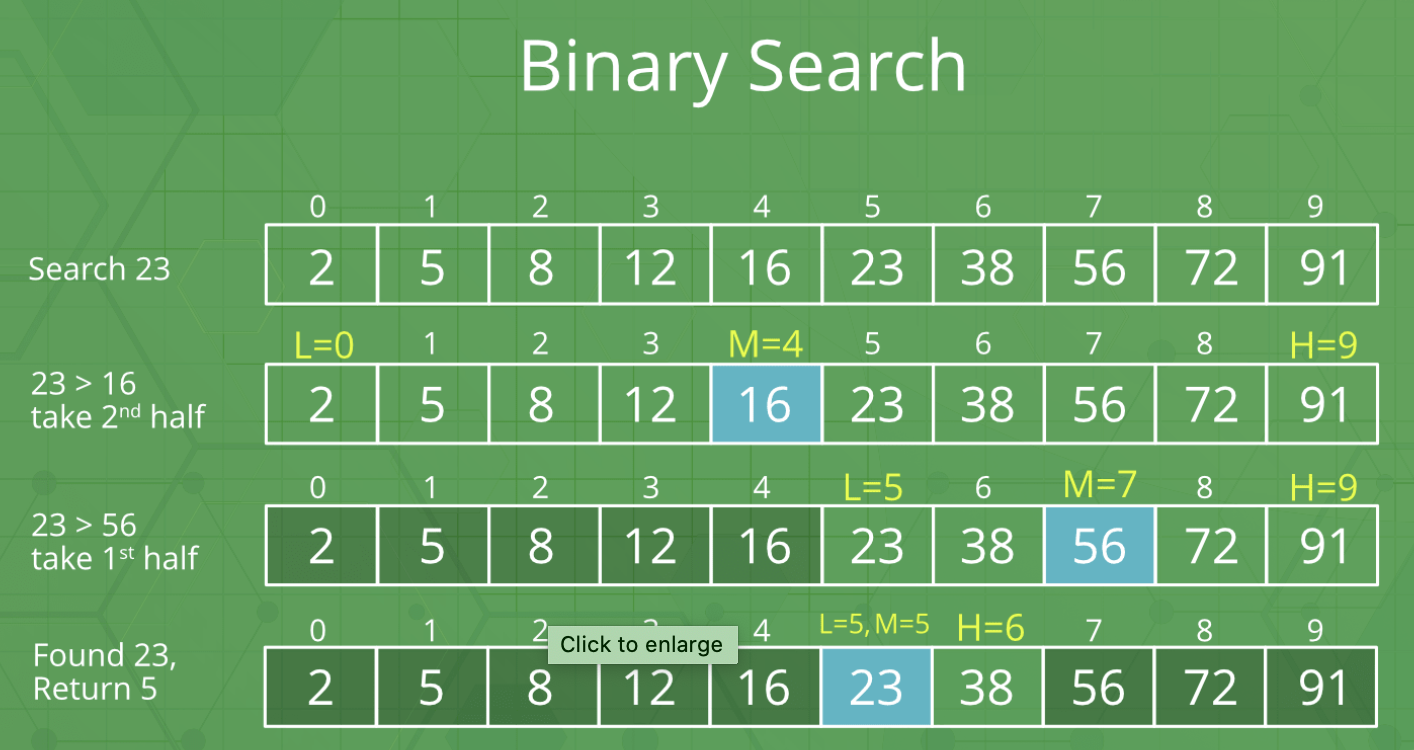
\includegraphics[width=\textwidth]{images/binary.png}
    \caption{An example of using binary search to find number 23 in the given array. \href{https://www.geeksforgeeks.org/binary-search/}{\textit{Source}}}
    \label{fig:binary}
\end{figure}


Below is an example implementation of binary search in Java.

\begin{code}
public class Example
{
    public static int binarySearch(int a, int b)
	{
	if (a-b == 1) return a;
 	int middle = a + (a-b)/2;
	StdOut.print("Is the secret number greater than or equal to " + middle + "? ");
	if (StdIn.readBoolean())
		return binarySearch(middle, b);
	else
		return binarySearch(a; middle);
	}
	public static void main(String[] args)
{
int k = Integer.parseInt(args[0]);
int n = (int) Math.pow(2, k);
StdOut.println("Choose a secret number between 0 and " + (n-1));
int guess = binarySearch(0, n)
StdOut.println("The secret number is " + guess);
}
}
\end{code}
 
 
 Mathematically, we can show that $T(n) = lg n$ where $T(n)$ is the number of questions. This, the running time of binary search is logarithmic.

\subsection{Binary search in a sorted array}
An important application of binary search is when we would like to find a piece of information using a key to guide the search. For example, in the last century people would use a phone book to look up a person’s phone number. In this case, the elements are sorted by a key (i.e. a person’s name, sorted in alphabetical order). Nowadays, we can implement this searching process using binary search.



\section{Insertion sort}

Now, we would like to discuss a few of the most fundamental sorting algorithms. 
Let’s start with a brute force algorithm known as \textit{insertion sort}. This algorithm mimics a method that people usually use to arrange hands of playing cards. Consider the cards one at a time and insert each into its proper place among those that have already been considered. Below is an example Java method that rearranges the strings in an array to put them in ascending order:

\begin{code}
public static void sort(String[] a)
{
	int n = a.length;
	for (int i = 1; i < n; i++)
		for (int j = i; j > 0; j- -)
			if (a[j-1].compareTo(a[j]) > 0)
				exchange(a, j-1, j)
			else break;

}
 
\end{code}
 
 
 At i-th iteration of the outer \textit{for} loop, the first I elements in the array are in sorted order; the inner \textit{for} loop moves a[i] into its proper position in the array. Note that the running time of insertion sort is sensitive to its input values. For example, if the input array happened to be already sorted, the running time of the program is linear. However, if the input array is in reversed order, then the running time is quadratic. There are many real-world applications for which insertion sort is quadratic, so we need to consider faster sorting algorithms.

\begin{figure}
    \centering
    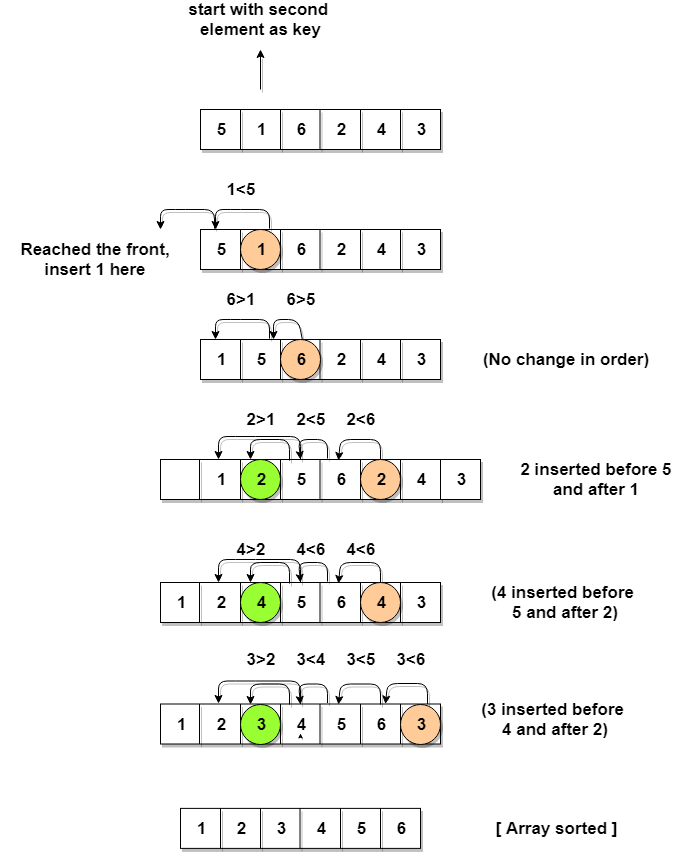
\includegraphics[width=\textwidth]{images/insertion-sort.png}
    \caption{An example showing how the insertion sort algorithm works. \href{https://vivaharsha.com/product/verilog-implementation-of-insertion-sort-16-bits-and-5-inputs/}{\textit{Source}}}
    \label{fig:insertion_sort}
\end{figure}


\section{Mergesort}
To create a faster sorting method, we need to understand recursion and a \textit{divide-and-conquer} approach to algorithm design. \textit{Divide-and-conquer} approach refers to the idea that we can solve a problem by \textit{diving} it into in depend parts, \textit{conquer} them independently, and then use the solution for the parts to develop a solution to the original problem. Applying this approach to sorting, we can first divide an array into two halves, sort the two halves independently, and then \textit{merge} the results into the full array. This sorting algorithm is called \textit{mergesort}. 

We consider contiguous subarrays of a given array \textit{array}, using the notation [a;b) to refer to the array consisting of elements array[a], array[a+1], …, array[b-1]. The mergesort algorithm implements the following strategy:
   
\begin{itemize}
\item \textit{Base case:} if the subarray length is 0 or 1, it is already sorted.
\item \textit{Reduction step:} If not, compute $middle = a + (a+b)/2$, recursively sort the two subarrays array[a, middle) and array[middle, b] and merge them.
\end{itemize}

You can view a short video that shows an example of how the mergesort algorithm works \href{https://youtu.be/4VqmGXwpLqc}{\textit{here}}.




\begin{exercise}

Fill in the blanks in the implementation of the mergesort algorithm.
\begin{code}

public void merge(int[] list, int low, int high) {
// temporary array stores the "merge" array within the method.

int[] temp = new int[list.length];
    // Set the midpoint and the end points for each of the subarrays
    int mid = (low + high)/2;
    int index1 = 0;
    int index2 = BLANK ;
    int index3 = mid + 1;
    // Go through the two subarrays and compare, item by item,
    // placing the items in the proper order in the new array
    while (index2 <= mid && index3 <= high) {
        if (list[index2] < list[index3]) {
            temp[index1] = list[index2];
            index1++;
            index2++;
}
else {
            temp[index1] = BLANK;
            index1++;
            index3++;
} }
    // if there are any items left over in the first subarray, add them to
    // the new array
    while (index2 <= mid) {
        temp[index1] = list[index2];
        index1++;
        index2++;
}
    // if there are any items left over in the second subarray, add them
    // to the new array
    while (index3 <= high) {
        temp[index1] = list[index3];
        index1++;
        index3++;
}
    // load temp array's contents back into original array
    for (int i=low, j=0; i<=high; i++, j++) {
        list[i] = BLANK;
    }
}

 
\end{code}
 

\end{exercise}
 
 Mathematically, we can show that the running time of mergesort is linearithmic.
 
 
 \section{Quicksort}
 
 
 Another sorting divide-and-conquer algorithm is called \textit{quicksort}. It works by \textit{partitioning} an array into two parts and then sorting the parts independently. The main feature of this sorting algorithm is the partiotioning process, which rearranges the array to make three conditions hold:

\begin{itemize}
\item The entry array[j] is in its final place in the array, for some j
\item No entry in array[a] through array[j-1] is greater than array[j]
\item No entry in array[j+1] through array[b] is less than array[j]
\end{itemize}

With this algorithm, we do the sorting by first partitioning the array and then applying this method recursively to the subarrays of the array. This algorithm shuffles the array before sorting it. 

\textbf{Partitioning} To implement the quicksort algorithm, we first need to implement the partitioning method. First, we arbitrarily choose array[a] to be the partitioning item, which will go into its final position. Next, we search from the left end of the array for an entry that is greater than or equal to the partitioning item. We then search from the right end of the array for an entry that is less than or equal to the partitioning item.The two found items are out of place so we exchange them. When the scan indices cross, to finish the partitioning process we need to exchange the partition item array[a] with the rightmost entry of the left subarray (array[j]) and return its index j.



You can view a short video that shows an example of how the quicksort algorithm works \href{https://youtu.be/Hoixgm4-P4M}{\textit{here}}.

\begin{figure}
    \centering
    \includegraphics[width=\textwidth]{images/quicksort.png}
    \caption{An example showing how the quicksort algorithm works. \href{https://runestone.academy/runestone/books/published/pythonds/SortSearch/TheQuickSort.html}{\textit{Source}}}
    \label{fig:insertion_sort}
\end{figure}


\begin{exercise}
Choose your favorite searching or sorting algorithm and run experiments with different input sizes to determine how the running time of the program changes with the input size. Run the algorithms on ten different input sizes and make a plot of the running time as a function of the input size.

\end{exercise}
	

\appendix
\addappheadtotoc
\appendixpage
	\section*{Possible appendices topics}

Hello, World.

\begin{figure}[h]
	\centering
	\includegraphics[width=0.85\textwidth]{images/hello_world_description}
	\label{fig:hello_world_description}
\end{figure}

Edit, compile, execute

\begin{figure}[h]
	\centering
	\includegraphics[width=0.85\textwidth]{images/edit_compile_execute}
	\label{fig:edit_compile_execute}
\end{figure}

Built-in data types

\begin{figure}[h]
	\centering
	\includegraphics[width=0.85\textwidth]{images/data_types}
	\label{fig:data_types}
\end{figure}

Booleans

\begin{figure}[h]
	\centering
	\includegraphics[width=0.85\textwidth]{images/booleans}
	\label{fig:booleans}
\end{figure}

Printing

System.out.print() is for regular printing
System.out.println() is same as System.out.print() but adds a newline
System.out.printf() prints \textbf{f}ormatted text, so you can easily insert data types inside a string and specify things like how many decimals should go after numbers. 
\begin{tabular}{|l|l|}
\hline
Format Specifier & Effect\\
\hline
\%s,\%S & Formats String\\
\%f & Formats floating point (precision provided between \% and f)\\
\%d & Formats integer\\
\%c & Formats character\\
\%b, \%B & Formats Boolean\\
\hline
\end{tabular}

Example: 

\begin{code}
System.out.printf("%.3f\n%.4f%d\n", 1.252525, 1.353535, 3);
\end{code}

prints 

\begin{code}
1.253
1.35353
\end{code}

\ja{todo: Scanners}

\ja{Cite https://introcs.cs.princeton.edu/java/11cheatsheet/}

\begin{itemize}

	\item Comparing floating point numbers.
	\item Type conversion.
	\item Useful math functions, e.g. \ic{min()}, \ic{log}.

\end{itemize}

\section{Java Reserved Words}

TODO: fill this in

\end{document}
